\documentclass[phd,tocprelim]{cornell}

\usepackage{dsfont}
\usepackage{amsmath, amsthm}
\usepackage{color}
\usepackage{float}
\usepackage[left=1.25in, bottom=1.5in, right=1.5in, top=1in]{geometry}
\usepackage{caption}

\usepackage{amsfonts}
\usepackage{times}
\usepackage{bm}
\usepackage{enumerate}
\usepackage{amssymb}
\usepackage{rotating} 
\usepackage{float}
\usepackage{bbm}
\DeclareMathVersion{normal2}
\mathversion{normal2} 
\mathversion{normal}
\usepackage{mathabx}
\usepackage{cite}
\usepackage{subcaption}
\captionsetup{compatibility=false}

\usepackage[square,sort,comma]{natbib}
\usepackage[toc,page]{appendix}
\usepackage{stmaryrd}
\usepackage{mathrsfs}
\usepackage[mathscr]{euscript}
\let\algorithmic\relax
\let\theoremstyle\relax

\usepackage[algo2e]{algorithm2e} 
\usepackage{algorithm}
\usepackage{algorithm, algpseudocode}
\usepackage{amsmath}
\usepackage{url}


\numberwithin{equation}{section}

\renewcommand{\labelenumi}{\theenumi}
%\theoremstyle{plain}
\newtheorem{thm}{Theorem}[section]
\newtheorem{cor}[thm]{Corollary}
\newtheorem{lem}[thm]{Lemma}
\newtheorem{assumption}[thm]{Assumption}
\newtheorem{prop}[thm]{Proposition}
\newtheorem*{remark}{Remark}
\newtheorem{definition}{Definition}[section]

%\newtheorem{proof}{Proof}

\newcommand{\var}{\mbox{Var}}
\newcommand{\cov}{\mbox{Cov}}
\newcommand{\rank}{\mbox{rk}}
\newcommand{\argmax}{\operatornamewithlimits{argmax}}
\newcommand{\argmin}{\operatornamewithlimits{argmin}}
\newcommand{\esssup}{\operatornamewithlimits{ess ~sup}}
\newcommand{\essinf}{\operatornamewithlimits{ess ~inf}}
\newcommand{\iu}{{i\mkern1mu}}
\newcommand{\E}{\mathbb{E}}
\newcommand{\Var}{\mathrm{Var}}
\newcommand{\Cov}{\mathrm{Cov}}
\newcommand{\Prob}{\mathbb{P}}
\newcommand{\T}[2][]{\boldsymbol{#1\mathscr{\MakeUppercase{#2}}}}
% matrices
\newcommand{\M}[1]{\mathbf{#1}}
% vectors
\newcommand{\V}[1]{\mathbf{#1}}
\newcommand{\vc}{\mathop{\mathbf{vec}}}
\newcommand{\real}{\mathbb{R}}





\newcommand{\beas}{\begin{eqnarray*}}
\newcommand{\eeas}{\end{eqnarray*}}
\newcommand{\bea}{\begin{eqnarray}}
\newcommand{\eea}{\end{eqnarray}}
\newcommand{\beq}{\begin{equation}}
\newcommand{\eeq}{\end{equation}}
\newcommand{\bit}{\begin{itemize}}
\newcommand{\eit}{\end{itemize}}
\newcommand{\ben}{\begin{enumerate}}
\newcommand{\een}{\end{enumerate}}


\newcommand{\cf}{cf.}
\newcommand{\eg}{e.g.}
\newcommand{\ie}{i.e.}
\newcommand{\etc}{etc.}
\def\reals{\mathbb{R}}

\newcommand{\vertiii}[1]{{\left\vert\kern-0.25ex\left\vert\kern-0.25ex\left\vert #1 
		\right\vert\kern-0.25ex\right\vert\kern-0.25ex\right\vert}}





\def\v{{\varepsilon}}




\graphicspath{{spectral/img/}{spectral/}{./adaptive/img/}{tensor/}{tensor/figure/}{projection/}{projection/figure/}{./}}

\newcommand{\colred}[1]{{\color{red}{#1} }}
\newcommand{\typo}[1]{\underline{\colred{#1}}}


\title {High Dimensional Data Analysis With Dependency and Under Limited Memory}
\author {Yiming Sun}
\conferraldate {September}{2019}
\degreefield {Ph.D.}
\copyrightholder{Yiming Sun}
\copyrightyear{2019}




\begin{document}
\maketitle

\makecopyright

\begin{abstract}
	Several methods for high dimensional analysis are proposed  in this thesis under the condition that there are data dependency and limited memory. The first part of the work proposes a model free method for building networks for time series data when data are dependent from weakly stationary time series. We develop a thresholding based on methods to estimate multivariate spectral density under weakly sparsity assumption for high dimensional time series.
	Our theoretical analysis ensures that consistent estimations of spectral density matrix of a p-dimensional time series using n samples
	are possible under high-dimensional regime $\log p/n \rightarrow 0$ as long as the true spectral density is approximately sparse. A key technical component of our analysis is a new concentration inequality of
	average periodogram around its expectation, which is of independent interest. Our estimation consistency results complement existing results for shrinkage based estimators of multivariate spectral
	density, which require no assumption on sparsity but only ensure consistent estimation in a regime
	$p^2/n \rightarrow 0$. In addition, our proposed thresholding based estimators perform consistent and automatic
	edge selection when coherence networks among the components of a multivariate time series are learned.
	We demonstrate the advantages of our estimators using simulation studies and a real data application
	on functional connectivity analysis with fMRI data. \par 
	We further show that with a simple modification in the classic estimator, we can build a rigorous theory for adaptive thresholding in estimating multivariate spectral density for Gaussian process. This adaptive estimator can capture the heterogeneity across different positions in spectral density matrix at a better convergence rate in comparison to the hard thresholding estimator.   \par 
	The second part delves into compressing/analyzing high dimensional data with limited memory. We fixate on developing a streaming algorithm for Tucker Decomposition, generalization of singular value decomposition. The method applies a randomized linear map to the tensor to obtain a \emph{sketch}
	that captures the important directions within each mode as well as the interactions among the modes.
	The sketch can be extracted from streaming or distributed data or with a single pass over the tensor which uses storage proportional to the degrees of freedom in the output Tucker approximation.
	Although the algorithm can exploit another view
	to compute a superior approximation, it does not require a second pass over the tensor. In conclusion, the paper provides a rigorous theoretical guarantee
	on elimination of the approximation error. Extensive numerical experiments show that the algorithm
	produces useful results that improve the state of the art for streaming Tucker decomposition. \par 
	Along the development of one-pass Tucke decomposition, we propose a memory efficient random mapping which we call Tensor random projection. We further study its theoretical property in application to several areas like random projection, sketching algorithms for fast computation for tensor regression. 
\end{abstract}

%\begin{biosketch}
%Your biosketch goes here. Make sure it sits inside
%the brackets.
%\end{biosketch}

\begin{dedication}
	To my parents 
\end{dedication}

\begin{acknowledgements}
	First and foremost, I would like to extend my sincere gratitude towards my PhD advisers, Sumanta Basu and Madeleine Udell for their guidance, time and commitment to my development towards an independent researcher. In particular, professor Udell's enthusiasm toward almost all novelties and energetic working style are an inspiration to me, while her ability to address numerous issues also leaves me a deep impression. I deeply appreciate the precious assistance my professor Udell offered who has quickly ushered me into new fields and provided me with insightful suggestions.
	 It is professor Basu that imparts the necessity of cooperation with people of different backgrounds like economics and biology to me.  I appreciate the precious assistance professor Basu offered who has taught me how to conduct research independently. \par 
	In addition, professor Michael Nussbaum and Yudong Chen always provide innovative and rigorous mathematical insights. I really appreciate that during the winter time, professor Nussbaum went through many results in spectral density estimation with me purely out of fervent devotion to researches. Every time talking with professor Yudong, I can learn many refreshing updates ranging from optimization, high dimensional statistics under various settings. \par 
	My heartfelt tribute would also be payed to the talented and intellectual people who have enlightened me during my PhD pursuit. I acquired the down to earth work ethics from Congzheng Song and Zhengqi Li, two PhDs in computer science who are my project partners. Ding Ma, who has already become an assistant professor, shared lots of her stories to assist me in facing uncertainties and anxiety in life. Lots of my old friends like Chengcheng Liu, Kuangyan Song always provides me with support. 
	
	During my several industrial interns, I was fortunate enough to be mentored by Olivia Simpson, Jessica Stauth, David Sargent etc.. What I appreciate the most is their genuine collaborative and caring working style besides numerous expertise that they have embedded in me. 
	
\end{acknowledgements}

\contentspage
\listoffigures
\listoftables

\normalspacing \setcounter{page}{1} \pagenumbering{arabic}
\pagestyle{cornell} \addtolength{\parskip}{0.5\baselineskip}








\chapter{Large Spectral Density Matrix Estimation by Thresholding}
\section{Introduction}\label{introduction}

Multivariate spectral density estimation is an important problem in time series and signal processing, with applications in many scientific disciplines including economics \citep{granger1969investigating}  and neuroscience \citep{bowyer2016coherence}. Spectral density of a stationary multivariate time series is the frequency domain analogue of covariance and is based on the Fourier transform of autocovariance function. It aggregates information on linear association, both contemporaneous and across different lags,  among the components of a multivariate time series. So it can be used to provide a richer description of cross-sectional dependency than Pearson correlation, which only accounts for contemporaneous association among the time series components. 

In particular, multivariate spectral density and coherence (frequency domain analogue of correlation) are routinely used in neuroscience as metrics of  functional connectivity among brain regions using time series of neurophysiological signals (e.g., fMRI, EEG and MEG) and to construct networks of interactions in a data-driven fashion \citep{bowyer2016coherence}. These connectivity networks, where each node corresponds to a brain region and edge weights correspond to strengths of coherence between regions, are often used to study differential brain connectivity patterns in patients suffering from neurological disorders. More recently, coherence metrics have also been used to construct similarity measures when clustering high-dimensional time series of brain signals \citep{euan2016hierarchical}. With advances in data collection and storage technologies, it is now feasible to analyze time series data on a large number of brain regions. For instance, the freeSurfer brain atlas used in this paper summarizes voxel level data to $p = 86$ brain regions. Consequently, there is an increasing interest among neuroscientists in constructing coherence networks among a large number of brain regions in a principled manner from temporally dependent samples of small to moderate size ($n \ll p^2)$. For instance, we use only $n=200$  samples for our fMRI data analysis in this paper.

This recent interest in learning the cross-sectional dependence from spectral density matrix at different frequencies is complementary to developments in classical time series and signal processing literature, which focused more on studying the \textit{shape} of spectral density function in a low-dimensional asymptotic regime ($p$ fixed, $n \rightarrow \infty$) \citep{brillinger1981time, brockwell2013time}.  In another line of work, \cite{dahlhaus1997identification, dahlhaus2003causality, eichler2007frequency} investigated in depth the issues of inference with coherence and testing of marginal independence between components of multivariate time series using integrated spectral density. Finer and uniform convergence rates of smoothed periodograms were more recently provided by \cite{wu2015uniform}. However, as the dimension of the time series increases, so does the estimation risk of smoothed periodograms. This was first pointed out by \cite{bohm2009shrinkage}, who showed that shrinking smoothed periodogram towards a simpler structure can reduce risk and make the estimates better-conditioned for studying inverse spectral density matrix. 
The authors also proved consistency of their estimates under a double-asymptotic regime $p \rightarrow \infty, n \rightarrow \infty, p^2/n \rightarrow 0$. In a series of papers, \citet{bohm2008structural,  fiecas2016dynamic,  fiecas2014datadriven} have made significant progress in this direction by providing a wide variety of shrinkage methods with attractive theoretical and empirical properties.

In this work, we make two additions  to this research direction of learning large spetral density matrices. First, we propose a family of \textit{sparsity regularized estimators} of spectral density matrix based on thresholding averaged periodograms. Our proposed estimators have the added advantage of performing  automatic edge selection and providing sparse, interpretable networks among the component time series. Second, we develop a non-asymptotic theory for estimation of  spectral density and coherence that explicitly connects estimation error bounds to a notion of approximate sparsity of the true spectrum. As a consequence, our theory shows that consistent estimation is possible in a high-dimensional regime $\log p / n \rightarrow 0$ as long as the underlying structure is approximately sparse. 

Our proposal is motivated by recent  developments in covariance matrix estimation literature, where several thresholding based strategies \citep{bickel2008covariance, rothman2009generalized, cai2011adaptive, cai2016rates} have shown to provide good theoretical and empirical properties compared to the shrinkage based estimators proposed in \citet{ledoit2004well}. The thresholding techniques developed in this literature serve as promising candidates for high-dimensional spectral density estimation as well. However, their implementation and theoretical analysis require addressing additional technical challenges. From an implementation consideration, choice of threshold in covariance matrix estimation for i.i.d. data is carried out using multiple sample-splitting \citep{bickel2008covariance} which is not feasible when the data have a temporal ordering. On the theoretical side, non-asymptotic analysis of  periodograms averaged across nearby frequencies requires understanding concentration behavior of a sum of random matrices that are \textit{neither independent nor identically distributed}. Unlike sample covariance estimation with i.i.d. data, the lack of identical distribution results in smoothing bias well-known in nonparametric density estimation. In addition, the additional temporal dependence complicates deriving finite sample deviation of averaged periodogram from its expectation. %Finally, analyzing finite sample concentration of averaged periodogram about its expectation require developing deviation bounds for quadratic forms of complex random variables currently not available in the literature. 

We make three technical contributions in this paper to address the above challenges. First, we select thresholding parameters using a frequency-domain sample-splitting scheme based on the heuristic of approximate independence of periodograms at different Fourier frequencies. Second, we provide upper bounds on the finite sample bias of averaged periodograms and provide insight into how it is affected by temporal dependence in data for some commonly used families of time series. Finally, we develop a non-asymptotic upper bound on the deviation of averaged periodogram using a Hanson-Wright type inequality for complex quadratic forms of temporally dependent random vectors. Building upon these technical ingredients, our main theoretical results include (i) consistency of thresholded averaged periodograms in operator and scaled Frobenius norms in a high-dimensional regime under a weak sparsity assumption on true spectrum, and (ii)  sparsistency results ensuring selection of marginally correlated pairs of time series in a coherence network with high probability. Our analysis  framework accommodates Gaussian time series, and linear processes with subGaussian or generalized subexponential errors, or errors with finite fourth moments. The rates of convergence of thresholded estimators change with the nature of tail distribution of errors.

We demonstrate the merits of our proposed methods using extensive numerical experiments and a real data application on constructing functional connectivity networks from fMRI data. Our numerical experiments show that thresholding methods achieve  estimation accuracy comparable with  the shrinkage method, while simultaneously performing automatic coherence selection. In particular, a  lasso and an adaptive lasso based thresholding strategy show promising performance across different simulation settings. In the real data application, these two methods were able to extract  sparse, interpretable networks that nicely captured known biological patterns in brain networks and distinguished different brain regions from each other.





The rest of the paper is organized as follows. In section \ref{sec:model-methods}, we formally introduce our problem, provide a brief review of shrinkage estimators, and describe our proposed thresholding methods. In section \ref{sec:theory}, we derive non-asymptotic upper bounds on our proposed spectral density estimates for Gaussian time series. In section \ref{sec:heavy-tail} we extend the results for Gaussian time series to general linear processes with different non-Gaussian noise distributions. In section \ref{sec:simulation}, we conduct simulation studies to assess the finite sample properties of our proposed estimators. Section \ref{sec:realdata} contains an empirical application of our proposed method to a functional connectivity analysis with real fMRI data. We defer the proofs of all of our technical results to the Appendix. 



\textbf{Notation.} Throughout this paper, $\mathbb{Z}$, $\mathbb{R}$ and $\mathbb{C}$  denote the sets of integers, real numbers and complex numbers, respectively. We use $|c|$ to denote the modulus of a complex number and the absolute value of a real number. We use $\|v\|$ to denote $\ell_2$-norm of a vector $v$. For a matrix $A$, $\|A\|_1$, $\|A\|_{\infty}$, $\|A\|$ and $\|A\|_F$ will denote maximum complex modulus column sum norm, maximum complex modulus row sum norm, { spectral norm} $\sqrt{\Lambda_{\max}(A^\dag A)}$ and Frobenius norm $\sqrt{\text{tr}(A^\dag A)}$, respectively, where $A^\dag$ is conjugate transpose of $A$. We also let $\lambda_{\text{max}}(A)$ denote the spectral radius of a $n \times n$ matrix $A$, i.e., $\lambda_{\text{max}}(A) = \max(|\lambda_1|, \cdots |\lambda_n|)$, where $\lambda_i$ are the eigenvalues of matrix $A$. If $A$ is symmetric or Hermitian, we denote its maximum and minimum eigenvalues by $\Lambda_{\min}(A)$ and $\Lambda_{\max}(A)$. We use $e_i$ to denote the $i^{th}$ unit vector in $\mathbb{R}^p$, for $i = 1, 2, \ldots, p$. For vectors $v_i \in \mathbb{R}^p, i=1,\ldots, n$, we use $[v_1:\ldots:v_n]$ to denote the $p \times n$ matrix formed  by horizontally stacking these column vectors $v_i$, and  $[v_1^\top;\ldots; v_n^\top]$ to denote the $n\times p$ matrix by vertically stacking row vectors $v_i^\top$. Let $vec(A)$ represent the vector got from vectorization of a matrix $A$ by stacking all its columns. We use $rk(A)$ to denote the rank of a matrix $A$. For a complex vector $v\in \mathbb{C}^p$ and any $q > 0$, we define $\|v\|_q:= (\sum_{i=1}^p |v_i|^q)^{1/q}$. We use $\|v\|_0$ to denote the number of non-zero elements in $v$. Note that when $0\le q<1$, it is not really a norm since triangle inequality does not hold, but we keep the notation of a norm for convenience . Then we define the induced matrix norm, $\|A\|_{\alpha, \beta} = \sup_{x\neq 0}\|Ax\|_\alpha/\|x\|_\beta$, for any  $\alpha>0, \beta>0$. We will also use $\|A\|_\alpha$ to denote the induced norm $\|A\|_{\alpha, \alpha}$ for any $\alpha > 0$ and any complex matrix $A \in \mathbb{C}^{p \times p}$. Also, to be succinct, we use $\|A\|_{\rm{max}} :=\max_{r,s}|A_{rs}|$. 
Throughout the paper, we write $A \succsim B$ if there exists a  universal constant $c > 0$, not depending on model dimension or any model parameters, such that $A \ge cB$. We use $A \asymp B$ to denote $A \succsim B$ and $B \succsim A$. 
% In spectral density estimation, $\Omega_n(f_X)$ and $L_n(f_X)$ will measure the estimation error of autocovariance which will be discussed in details later. 

\iffalse
{\color{red} [Note: motivate weak sparsity; highlight contribution of new tuning parameter selection method in freq domain; see if bringing description of shrinkage methods in here makes sense; after simulation, add discussion of heterogeneity in addition to weak sparsity; do careful literature search about other competing shrinkage methods; add success stories of coherence metrics in neuroscience].}
\begin{enumerate}
    \item propose (soft/hard)-thresholding based spectral density estimates which comes with automatic variable selection (rather than shrinkage);
    \item non-asymptotic theoretical analysis that holds in high-dimensional regime $\log p /n \rightarrow 0$ under weak sparsity; results hold for linear processes with non-Gaussian errors; general purpose concentration bounds involving DFT, useful in other contexts as well (approximate independence of DFT's generalize to high-dim setting, also joint guaranteee across m frequencies -- check Wei Biao's paper for other usage of such a result); require finite sample analysis of bias since tuning parameter choice depends on it;
    \item novel method of tuning parameter selection;
    \item numerical evidence supporting the merit of thresholding approach for heterogeneous structures;
    \item Application to real EEG data [findings].
\end{enumerate}
\fi










\section{Background and Methods}\label{sec:model-methods}
Consider a $p$-dimensional weakly stationary real-valued time series $X_t = (X_{t1}, \ldots, X_{tp})^\top, ~ t\in \mathbb{Z}$. Let  $\mathcal{X} = [X_1:\ldots:X_n]^\top$  be the \textit{data matrix} containing $n$ consecutive observations from the time series $\{X_t\}$ in its rows. We assume $\mathbb{E} X_t = 0, ~ t=1,\ldots,n$ for ease of exposition. In practice, multivariate time series are often de-meaned before performing correlation based analysis. Weak stationarity implies that $\cov(X_t, X_{t-\ell}) = \mathbb{E} X_t X_{t-\ell}^\top$ only depends on $\ell$, so we can define autocovariance as function of the lag $\ell$, viz., $\Gamma(\ell) = \cov(X_t, X_{t-\ell})$. Spectral density aggregates information of autocovariance of different lag orders $\ell$  at a specific frequency $\omega \in [-\pi, \pi]$ as 
\begin{equation}
f(\omega) = \frac{1}{2\pi}\sum_{\ell=-\infty}^\infty \Gamma(\ell) e^{-\iu \ell \omega }. 
\end{equation}
Note that the autocovariance functions of different lags can be recovered from the spectral density using the transformation  $\Gamma(\ell) =  \int_{-\pi}^{\pi} f(\omega) e^{i\ell \omega} d\omega$, for any $\ell \in \mathbb{Z}$.



For the matrix-valued spectral density function $f$ over $[-\pi, \pi]$, we define, for $q \ge 0$,
\begin{equation}
\vertiii{f}_q = \esssup_{\omega \in [-\pi, \pi]}\|f(\omega)\|_q. \nonumber
\end{equation}
Following \cite{Basu2015}, we will also use 
$\vertiii{f}: = \vertiii{f}_2 = \esssup_{\omega \in [-\pi, \pi]}\|f(\omega)\| $
as a measure of stability of the time series $X_t$. Larger values of $\vertiii{f}$ are associated with processes having stronger temporal and cross-sectional  dependence and less stability. Since every coordinate of the spectral density matrix is calculated using at most two components of the $p$-dimensional time series $X_t$ and $f(\omega)$ is non-negative definite, a smaller measure of stability, viz. $\max_{1 \le r \le p} \esssup_\omega \|f_{rr}(\omega)\|$ can be also used in our error bound analysis instead, although we present our results in terms of $\vertiii{f}$ for ease of exposition.

In many applications, in particular functional connectivity analyses in neuroscience, it is of interest to estimate standardized spectral density or coherence matrix, an analogue of correlation in the frequency domain,  defined as 
\begin{equation}
\label{def:coherance}
g_{rs}(\omega) = \frac{f_{rs}(\omega)}{\sqrt{f_{rr}(\omega)f_{ss}(\omega)}},
\end{equation}
assuming $f_{rr}(\omega) \neq 0$ for all $1\le r\le p$. 


\subsection{Background: Periodogram Smoothing and Shrinkage}\label{sec:model_method_background}


\begin{algorithm2e}[t]\small
	\DontPrintSemicolon 
	\KwIn{$j, m, N$, periodograms at Fourier frequency $\{ I(\omega_k) \}_{k \in F_n}$, finite grid of thresholds $\mathcal{L}$}
	\For{$\lambda \in \mathcal{L}$}{
		\For{$\nu \gets 1$ \textbf{to} $N$}{
			Randomly divide $\{j-m, \ldots, j, \ldots, j+m\}$ into two subsets $J_1$ and $J_2$ such that $\left||J_1| - |J_2| \right| \le 1$ and for any $k \in F_n$, $k \in J_1$ iff $-k \in J_1$ \;
			$\hat{f}_{1, \nu} (\omega_j) \gets \sum_{k \in J_1} I(\omega_k)$, ~~ $\hat{f}_{2, \nu} (\omega_j) \gets \sum_{k \in J_2} I(\omega_k)$\;
			$\hat{R}_{\nu}(\omega_j, \lambda) \gets \left\| T_\lambda (\hat{f}_{1,\nu} (\omega_j)) - \hat{f}_{2,\nu}(\omega_j)\right\|^2_F$\;
		}
		$\hat{R}(\omega_j, \lambda) \gets \sum_{\nu=1}^N \hat{R}_{\nu}(\omega_j, \lambda) / N$
		
	}
	\KwOut{$\hat{\lambda}_j := \hat{\lambda}(\omega_j) = \argmin_{\lambda \in \mathcal{L}} \hat{R}(\omega_j, \lambda)$}
	\caption{Threshold Selection by Frequency Domain Sample-splitting}
	\label{alg:sample-split}
	\label{al1}
\end{algorithm2e}

The classical estimate of spectral density is based on the periodogram \citep{brockwell2013time, rosenblatt1985stationary} defined as
\begin{equation}
\label{eq:single_periodogram}
I(\omega)=\sum_{|\ell|<n} \hat{\Gamma}(\ell)e^{-\iu\ell\omega},
\end{equation}
where $\hat{\Gamma}(\ell) = n^{-1}\sum_{t=\ell+1}^{n} X_t X_{t-\ell}^\top$ for $\ell\ge 0$, and 
 $\hat{\Gamma}(\ell) = n^{-1}\sum_{t=1}^{n+\ell} X_t X_{t-\ell}^\top$ for $\ell<0$. 
Note the connection between periodogram and discrete Fourier transformation (DFT)  $d(\omega) = \mathcal{X}^\top(C(\omega)-iS(\omega))$ , where 
\begin{equation}
\label{eq:cos_sin_coef}
\begin{aligned}
C(\omega) = \frac{1}{\sqrt{n}} (1, \cos \omega, \dots, \cos (n-1)\omega)^\top,\\
S(\omega) = \frac{1}{\sqrt{n}} (1, \sin \omega, \dots, \sin (n-1)\omega)^\top.
\end{aligned}
\end{equation}
% For brevity, we write $C_j$ for $C_j(\omega)$ throughout the technical sections. 
We can rewrite $I(\omega)$ as $d(\omega) d(\omega)^\dag$. 
%It is customary to use these frequencies since we get some orthogonal discrete Fourier coefficient detailed discussed in lemma \ref{lemma:orthogonal-cos-sin}. Orthogonality here brings great convenience in building lemma \ref{lemma:maximum_L2_Q}. 
In classical asymptotic analysis of time series ($p$ fixed, $n \rightarrow \infty$), it is known that $\frac{1}{2\pi}I(\omega)$ is asymptotically unbiased for $f(\omega)$ but not consistent due to non-diminishing variance.
For instance, for i.i.d Gaussian white noise  
$X_t \overset{i.i.d}{\sim}\mathcal{N}(0,\sigma^2I)$, the variance of $I(\omega)$ is of the order $\sigma^4$ [Proposition 10.3.2,  \citet{brockwell2013time}].  To achieve consistency, it is common to resort to smoothing periodograms over nearby frequencies. In this paper, we focus on the simplest form of smoothing, viz. averaging, of periodograms 


\begin{equation}
\label{eq:general_smoothing_estimator}
    \hat{f}(\omega; m) = \frac{1}{2\pi(2m+1)} \sum_{|k|\le m} I(\omega+\omega_k),
\end{equation}
where $\omega_k = 2\pi k/n, ~ k\in F_n$,  the set of Fourier frequencies. To be precise, $F_n$ denotes the set  $\left\{-[\frac{n-1}{2}], \dots, [\frac{n}{2}]\right\}$ where $[x]$ is the integer part of $x$. $F_n$ contains exactly the same frequencies used to calculate discrete Fourier transformation. It is common to evaluate the periodogram at these Fourier frequencies, in which case the smoothing periodogram in \eqref{eq:general_smoothing_estimator} becomes
\begin{equation}
\label{eq:smoothing estimator}
    \hat{f}(\omega_j; m) = \frac{1}{2\pi(2m+1)} \sum_{|k|\le m} I(\omega_{j+k}).
\end{equation}
Note that even though the values of $j+k$ can fall outside $F_n$, it is enough to evaluate periodograms at Fourier frequencies $F_n$ since $I(\omega)$ is $2\pi$-periodic in $\omega$. Theorem 10.4.1 in \citet{brockwell2013time} shows that if $m = o(\sqrt{n})$, \eqref{eq:smoothing estimator} is a consistent estimator. As in general nonparametric function estimation, one can replace the weights $1/(2m+1)$ in \eqref{eq:smoothing estimator} by a more general kernel function. For more details, we refer the  readers to \cite{brockwell2013time}. To make notations simpler, in this paper we will omit the subscript $m$ and use $\hat{f}(\omega_j)$ whenever $m$ is clear from the context. 

%[{\color{red}{Add details on Shrinkage Estimation}}]
\par
This nonparametric smoothing method can be unstable for high-dimensional multivariate spectral density estimation since smoothed periodograms start to become ill-conditioned. Generalizing shrinkage estimation strategy for high-dimensional covariance matrix \citep{ledoit2004well}, \citet{bohm2009shrinkage} proposed shrinking averaged periodogram to estimate spectral density in high-dimension. The idea of shrinkage method is to reduce condition numbers for smoothed periodograms. In particular, the authors changed the estimation target to $f^0(\omega) = \mathbb{E} \hat{f}(\omega)$ and argued that $f^0(\omega)$ is close enough to $f(\omega)$ asymptotically. Subsequently, they considered a Hilbert space for square complex random matrices with inner product defined as  $\mathbb{E}\langle A,B\rangle$ where $A,B$ are two  matrices and 
\begin{equation}
\langle A,B \rangle = \frac{1}{p} \text{tr}(A^\dag B).\nonumber %, ~~~~ \|A\|^2 = \left[ \frac{1}{p} \text{tr}(A^\dag A)\right]. 
\end{equation} 
In this Hilbert space and with the fact that $\hat{f}(\omega)$ is an unbiased estimator for $f^0(\omega)$,  \citet{bohm2009shrinkage} applied the projection argument similar to \citet{ledoit2004well} to build the shrinkage estimator for $f^0(\omega)$. To this end, the authors first projected $f^0(\omega)$ on the space spanned by the identity matrix as $\mu(\omega) I_p$, where $I_p$ is the identity matrix and $ \mu(\omega)= \frac{1}{p} \text{tr}(f(\omega))$. Then the shrinkage estimator is defined as the minimizer of the convex program 
\begin{equation}
\hat{f}^\star(\omega) = \argmin_{\tilde{f}(\omega) \in S(\omega)} \frac 1 p \|f^0(\omega) - \tilde{f}(\omega)\|^2_F, \nonumber
\end{equation}
where 
\begin{equation}
S(\omega) = \rho(\omega) \mu(\omega)I_p + (1-\rho(\omega)) \hat{f}(\omega), ~~~~ 0\le \rho(\omega)\le 1. \nonumber
\end{equation}
\citet{bohm2009shrinkage} derived an explicit formula 
%of $\rho$:
%\begin{equation}
$\rho(\omega) = {\alpha^2(\omega)}/{\delta^2(\omega)}$,
%\end{equation}
where 
\begin{equation*}
    \alpha^2(\omega) = \frac 1 p \|f^0(\omega) - \mu(\omega)I_p\|^2_F,~~
    \beta^2(\omega) = \frac 1 p \|f^0(\omega)-\hat{f}(\omega)\|^2_F,
\end{equation*}
and $\delta^2(\omega) = \alpha^2(\omega)+\beta^2(\omega)$. 
\iffalse
\begin{equation}
\begin{aligned}
&\alpha^2(\omega) = \frac 1 p \|f^0(\omega) - \mu(\omega)I_p\|^2_F,\\
&\beta^2(\omega) = \frac 1 p \|f^0(\omega)-\hat{f}(\omega)\|^2_F,\\
& \delta^2(\omega) = \alpha^2(\omega)+\beta^2(\omega).
\end{aligned}
\end{equation}
\fi
Then they plugged in estimators of $\alpha(\omega), \beta(\omega), \delta(\omega)$ into the above formula to get the final data-driven estimator of spectral density. \par

\subsection{Method: Thresholding Averaged Periodogram} \label{sec:method_threshold}
In this section, we present our proposed thresholding estimators. We restrict our methodology description and theoretical development on the finite grid of Fourier frequencies for convenience, although all our theoretical results hold for any arbitrary frequency $\omega \in [-\pi, \pi]$. We briefly explain why all theoretical developments still hold for thresholding on smoothed periodograms at a  general frequency defined in \eqref{eq:general_smoothing_estimator}. The key property we used to develop error bound analysis for thresholding estimators is orthogonality of $d(\omega_j), j\in F_n$. For general frequency $\omega$, we can show that $d(\omega+\omega_j), j=-m,\cdots, 0, \cdots, m$, are also orthogonal to each other. Based on this property, we could follow all arguments for Fourier  frequencies to achieve the same theoretical results. 


We propose \textit{\underline{hard thresholding}} of averaged periodograms, i.e., 
\begin{equation}
T_{\lambda}(\hat{f}_{rs}(\omega_j))= \begin{cases}
\hat{f}_{rs}(\omega_j) & \mbox{ if } |\hat{f}_{rs}(\omega_j)|\ge \lambda \\
0 & \mbox{ if } |\hat{f}_{rs}(\omega_j)| < \lambda,
\end{cases}
\end{equation}
where $\lambda > 0$ is a threshold chosen by the user, and can potentially be a frequency dependent number $\lambda_j$. $T_\lambda(\cdot)$ is a thresholding operator on spectral density, $T_{\lambda}(\hat{f}_{rs}(\omega_j))$ represents the $(r,s)^{th}$ element of the thresholded matrix, where $1 \le r, s \le p$. For notational convenience, we will often use $\hat{f}_{\lambda, rs}(\cdot)$ instead of $T_{\lambda}(\hat{f}_{rs}(\cdot))$.

Following \citet{rothman2009generalized},  we also propose a variety of \textit{\underline{generalized thresholding operators}} $S_\lambda(.)$ that combine the benefits of shrinkage and thresholding. In particular, we consider elememt-wise shrinkage operator $S_\lambda(.)$ satisfying the following three conditions for any $z \in \mathbb{C}$: 
\begin{enumerate}[(1)]
\item $|S_\lambda(z)|\le |z|$,
\item $S_\lambda(z) = 0$ if $|z|\le \lambda$,
\item $|S_\lambda(z)-z|\le \lambda $.
\end{enumerate}
Similar to hard thresholding $T_\lambda(.)$, we apply this operator to individual elements of averaged periodogram. It turns out conditions (1)-(3) are satisfied by a number of thresholding and shrinkage procedures. 
% Here we deal with complex numbers, thus we may have more ways to define thresholding and shrinkage procedure. \cite{rothman2009generalized} presents two commonly used examples: soft thresholding (or lasso) and adaptive lasso for real numbers which may be extended to complex number case. 
In particular, the hard thresholding operator $T_\lambda(.)$ satisfies these conditions. In addition, generalizing \citet{rothman2009generalized} to the case of complex variables, we propose a soft thresholding (lasso) operator  
\begin{equation}
S_\lambda^s(z) = \frac{z}{|z|} \left(|z|-\lambda\right)_+, ~~ z \in \mathbb{C}, \nonumber
\end{equation}
and adaptive lasso operator 
\begin{equation}
S_\lambda^{\text{AL}} = \frac{z}{|z|} \left(|z| - \lambda^{(\eta+1)}|z|^{-\eta}\right)_+,  ~~ z \in \mathbb{C}. \nonumber
\end{equation}

Our proposed hard and soft thresholding procedures require selection of two tuning parameters: (i) smoothing span $m$ and (ii) level of threshold $\lambda$. In Section \ref{sec:theory}, we provide a detailed discussion of the theoretical choices of these parameters that ensure consistent estimation in high-dimensional regime. In the next subsection \ref{sec:tuning-parameter}, we discuss how to choose these two parameters in a data-driven fashion. The adaptive lasso based soft thresholding method has a third tuning parameter $\eta$. In our numerical and real data analyses, we set $\eta = 2$ following the suggestion of \cite{rothman2009generalized}, although a more general sample-splitting based choice along the line of Algorithm \ref{al1} can be adopted in practice.

\smallskip

When the thresholded spectral density matrices are sparse, they can be used to construct networks to visualize and analyze marginal dependence relationships among the component time series. However, just like thresholded covariance matrix estimators, thresholding individual entries does not necessarily ensure that the thresholded spectral density matrix estimate is positive definite. Our operator norm consistency results in Section \ref{sec:theory} implies that as long as the true spectral density is positive definite and the sample size is large enough, the thresholded estimate is positive definite with high probability. However, in finite sample, this is a limitation since the estimates cannot be directly used to calculate inverse spectral density and partial coherence. On the other hand, regularization is required to calculate inverse spectral density in high-dimension, and a more principled approach along the line of graphical lasso can be used to directly regularize entries of the inverse spectral density \citep{jung2015learning, jung2015graphical}. We expect that the key concentration inequalities developed in our analysis will be useful in the estimation of inverse spectral density as well.


\iffalse
In order to take the heterogeneity of cross-spectral density across different coordinates of the spectral density matrix into consideration, we develop a strategy simiilar to adaptive thresholding proposed in \citet{cai2011adaptive}, where the thresholds are  proportional to the variances of the elements at different positions. Formally, the adaptive threshold for position $r,s$ at frequency $\omega_j$ is defined as  
\begin{align*}
    \lambda_{j(r,s)} = \delta_j\sqrt{\frac{\theta_{(r,s)}\text{log }p}{n}}, ~~~~\mbox{ for all $\omega_j$}
\end{align*}
where $\theta_{(k,l)} := Var(\hat{f}_{(k,l)})$ which also needs to be estimated and $\delta_j$ is a tuning parameter. 
\fi

 
\subsection{Choice of Tuning Parameters}\label{sec:tuning-parameter}
At any Fourier frequency $\omega_j$, we need to choose two tuning parameters for our method - (i) the smoothing span $2m+1$, and (ii) the threshold level $\lambda$. In this work, we select a single smoothing span for all the frequencies, but choose the threshold level separately for each frequency.

% The first one is the smoothing bandwidth $2m + 1$. 
%The smoothing method is running average. {\color{red} Provide formula, or refer to equation number in introduction section.}
The smoothing span plays the role of ``effective sample size'' in estimating $f(\omega_j)$. Recall that 
\begin{equation}
    \hat{f}(\omega_j; m) = \frac{1}{2\pi (2m+1)} \sum_{|k|\le m} I(\omega_{j+k}). \nonumber
\end{equation}
In classical asymptotics ($p$ fixed, $n \rightarrow \infty$) and the Kolmogorov asymptotics ($p \rightarrow \infty, n \rightarrow \infty, p^2/n \rightarrow 0$) \citep{brockwell2013time, bohm2009shrinkage}, it is shown that for $\hat{f}(\omega_j; m)$ to be consistent, $m$  (depending on $n$) must go to infinity and $m/n \rightarrow 0$ as $n\rightarrow \infty$. Our non-asymptotic analysis in Section \ref{sec:theory} suggests that $m/[n\Omega_n(f)]  \rightarrow 0$, where $\Omega_n(f)$, defined as $\max_{r,s} \sum_{\ell=-n}^n |\ell| |\Gamma_{rs}(\ell)|$ is a measure of temporal dependence in the time series. For our numerical and real data applications, we choose $m$ in the order of  $\sqrt{n}$, with smaller values of $m$ for processes with stronger temporal dependence and larger $\Omega_n(f)$. A more data-driven approach along the line of \cite{ombao2001smoothing} and \citet{fiecas2014datadriven} can be designed with suitable modification to account for high-dimensionality, although we do not pursue this direction in this work.




The second tuning parameter is the threshold value. Unlike the shrinkage estimators of spectral density matrices, finding  asymptotically optimal plug-in estimators for threshold level is challenging due to the non-smooth nature of thresholding operators. For covariance estimation from  i.i.d. data using thresholding, a sample-splitting method proposed in \citet{bickel2008covariance} or its variants are normally employed. In this method, the entire sample is split into two sub-samples, and the Frobenius norm difference between thresholded estimation in one sub-sample and regular sample covariance in the other sub-sample is compared for different levels of threshold. The entire exercise is repeated $N$ times and the level of threshold minimizing the average Frobenius norm difference is selected as the threshold.

This approach is not directly amenable to spectral density estimation since for any two given sub-sample sizes, only $N=1$ split is possible maintaining the temporal ordering. However, the periodograms at different positive Fourier frequencies $\omega_j \in F_n, \omega_j \ge 0$, are asymptotically independent. This suggests an analogous sample-splitting algorithm can be designed in the frequency domain. With this heuristic, we propose the following algorithm.

For each frequency $j$ $\in \{1, \cdots, [n/2]\}$, we randomly split the periodograms in $\{j-m ,\cdots,j+m\}$ into two sub-samples $J_1, J_2$ of size $m_1$ and $m_2$, where $|m_1 - m_2 | \le 1$. Since $I(\omega_{-k}) = I(\omega_{k})$, we keep $I(\omega_k)$ and $I(-\omega_k)$ in the same sub-sample. Then, for every $\lambda$ on a finite grid of possible threshold choices $\mathcal{L}$, we calculate the squared Frobenius norm of the difference between thresholded averaged periodogram on $J_1$, viz.,  $\hat{f}_{1}(\omega_j)$,  and averaged periodogram $\hat{f}_{2}(\omega_j)$ on $J_2$. This exercise is repeated $N$ times and the threshold $\lambda \in \mathcal{L}$ minimizing squared Frobenius norm is selected as $\hat{\lambda}_j$ for frequency $\omega_j$. A complete description is provided in Algorithm \ref{al1}.







\section{Theoretical Properties}\label{sec:theory}
In this section, we analyze asymptotic properties of thresholded averaged periodograms under high-dimensional regime. In particular, we derive non-asymptotic upper bound on the estimation error under operator and Frobenius norms and relate them to a notion of weak sparsity of the spectral density matrices. A key technical ingredient of our analysis is a concentration inequality of complex quadratic forms of temporally dependent Gaussian random vectors. In section \ref{sec:heavy-tail} we extend these results to linear processes with more general noise distributions, including subGaussian and   subexponential families.

In contrast with classical asymptotic framework where $p$ is fixed and $n \rightarrow \infty$, a non-asymptotic analysis for high-dimensional time series requires careful quantification of the convergence rates, in particular how they are affected by cross-sectional and temporal dependence inherent in the time series. Therefore, before proceeding with the main theoretical results, we describe parameters of the multivariate time series $X_t$ that appears in our estimation error bounds.

\smallskip
\noindent \textbf{Weak Sparsity of Spectral Density: } 
In order to make meaningful estimation in a high-dimensional regime, we focus on a class of spectral density matrices with suitable low-dimensional structure of \textit{weak sparsity} measured by $\vertiii{f}_q$ for some $0 \le q < 1$. Matrices with small $\vertiii{f}_0$  are \textit{exactly sparse}, while small  $\vertiii{f}_q$ correspond to matrices within a small $\ell_q$ ball in $\mathbb{C}^{p\times p}$. Weak sparsity of regression coefficients and covariance matrices have been proposed earlier in \cite{van2016lecture} and \citet{bickel2008covariance} respectively. 
%low \cite{van2016lecture} discuss the weak sparsity measure in vector case thoroughly by defining $\rho^q = \sum_{i=1}^p |v_i|^q$ with $0\le q<1$ for vector $v\in \mathbb{C}^p$ and connecting it to lasso theory. For matrix case, \citet{bickel2008covariance} use $\max_{r=1}^p \sum_{s=1}^p |f_{rs}(\omega)|^q$ to measure weak sparsity.
% This generalizes the notion of \textit{exact} sparsity, allowing for many small non-zero coefficients in the matrix.
Weakly sparse covariance matrices have been applied to climate studies according to \cite{cai2016rates} and gene expression array analysis, as mentioned in \cite{cai2012minimax}. \par 

Although the induced norm defined in notation section does not satisfy triangle inequality for $0\le q<1$, $\|A\|_q^q$ satisfies the triangle inequality leading to 
\vspace{-0.1in}
\begin{equation}
\max_{s=1}^p \sum_{s=1}^p |f_{rs}(\omega)|^q = \|f(\omega)\|_q^q  \le \vertiii{f}_q^q, \nonumber
\end{equation}
where $\vertiii{f}_q = \esssup_{\omega\in [-\pi, \pi]} \|f(\omega)\|_q$ as defined before. 
We provide a proof of this statement in lemma   \ref{lemma:q_norm_eq}. 
Since spectral density $f(\omega)$ is a Hermitian matrix, $\vertiii{f}_q^q$ also measures the row weak sparsity. This weakly sparse class covers a  variety of sparse patterns as shown in \citet{bickel2008covariance}. 
%However, \citet{bickel2008covariance} requires diagonal entries of the covariance matrix  to be uniformly bounded above, i.e., $\Sigma_{rr}\le M$, $r = 1,\cdots p$.
%, where $\Sigma$ is the covariance matrix and $M$ is some general constant which is necessary for building concentration inequality for deviation from sample covariance matrix to population covariance matrix. 
%In our case, $\vertiii{f}$ already controls magnitude of diagonal elements since for any $f_{rr}(\omega), \omega \in [-\pi,\pi], 1\le r\le p$, 
%\begin{equation}
%\vertiii{f}\ge \|f(\omega)\|\ge |f_{rr}(\omega)|. \nonumber
%\end{equation} We will only consider stable time series assuming finite $\vertiii{f}$, or  slow growth rate of $\vertiii{f}$. It may be possible to relax this assumption by resorting to adaptive thresholding proposed by \cite{cai2011adaptive}, although we do not explore this direction in this work.

\smallskip
\noindent \textbf{Strength of Temporal and Cross-sectional Dependence: } %We consider a data matrix $\mathcal{\mathcal{X}} = [{X}_1:\ldots:{X}_n]^\top$ from a $p$-dimensional weakly stationary, zero-mean  time series. Consider $\hat{f}(\omega_j)$, the averaged periodogram defined in \eqref{eq:smoothing estimator}. To guarantee $\hat{f}(\omega_j)$ is a consistent estimator, 
The decay rates of the strengths of cross- and autocorrelation between components of $X_t$ capture the strength of temporal and cross-sectional dependence in data, which in turn relates to the effective sample size and appear in our error bounds. For meaningful estimation, we restrict ourselves to the class of short-range dependent time series $X_t$ with  the following summability assumption on its underlying autocovariance function $\Gamma(\ell)$:
\begin{assumption}\label{assumption:finite_auto}
$\sum_{\ell=-\infty}^\infty \|\Gamma(\ell)\|_{\text{max}}<\infty$. 
\end{assumption}

\noindent Under this assumption, we will present our bounds in terms of three quantities. The first one is $\vertiii{f}$ defined before, and will be used to assess the \textit{concentration of averaged periodogram around its expectation}. Note that $\vertiii{f}$ is finite since  
\begin{equation}
\|f(\omega)\| = \left\|\sum_{\ell = -\infty}^\infty \Gamma(\ell) e^{-\iu \omega \ell }\right\| \le \sum_{\ell = -\infty}^\infty \|\Gamma(\ell)\| \le \sum_{\ell=-\infty}^\infty p\|\Gamma(\ell)\|_{\rm{max}}.
\end{equation}
% which ensures that the spectral density is well defined. 
%Then
%\begin{equation*}
%\vertiii{f} = \esssup_{\omega \in [-\pi, \pi ]}\|f(\omega)\| <\infty. % = \sup_{\omega \in [-\pi, \pi ]}\|f(\omega)\|
%\end{equation*}
The other two quantities that capture the strength of temporal and contemporaneous dependence in the multivariate time series $\{X_t\}_{t \in \mathbb{Z}}$ are 
\begin{eqnarray}
\Omega_{n}(f) = \max_{1 \le r,s \le p} \sum_{\ell=-n}^n |\ell| |\Gamma_{rs}(\ell)|, ~~~~ L_n(f) = \max_{1 \le r,s \le p}\sum_{|\ell|>n} |\Gamma_{rs}(\ell)|.
\end{eqnarray}
Together, these two quantities help assess  how the \textit{bias of averaged periodogram} depends on the the degree of decay of the autocovariance function with increasing lag order $\ell$. Under Assumption \ref{assumption:finite_auto}, both of these quantities are finite. In Proposition \ref{prop:order_bias}, we show how these quantities grow for some common classes of multivariate time series.

\subsection{Estimation Consistency: Stable Gaussian Time Series} 

We start with a key technical ingredient of our analysis, a  Hanson-Wright type inequality \citep{rudelson2013hanson} for quadratic forms of random vectors generated by a multivariate Gaussian time series. This result generalizes Proposition 2.4 in \cite{Basu2015} by allowing an arbitrary matrix $A$ in the quadratic form. In Section \ref{sec:heavy-tail}, we extend this inequality to accommodate more general non-Gaussian time series.

Our modified Hanson-Wright inequality is crucial for understanding the concentration behaviour of averaged periodograms around the true spectral density $\left| \hat{f}_{rs}(\omega_j) - f_{rs}(\omega_j) \right|$, for a fixed coordinate $(r,s)$ of the $p\times p$ spectral density matrix. This deviation is required for selecting threshold $\lambda$ that ensures consistency in high-dimension. Unlike high-dimensional covariance estimation problem where sample covariance is an unbiased estimator of population covariance, the averaged periodogram at frequency $\omega_j$ is a biased estimator of $f(\omega_j)$. This requires developing upper bounds on both the ``bias'' and ``variance'' terms in the deviation of $\hat{f}_{rs}$ around $f_{rs}$: 
\begin{equation}
\left|\hat{f}_{rs}(\omega_j) - f_{rs}(\omega_j)\right| \le \left|\mathbb{E}\hat{f}_{rs}(\omega_j) - f_{rs}(\omega_j)\right| + \left| \hat{f}_{rs}(\omega_j) - \mathbb{E}\hat{f}_{rs}(\omega_j) \right|. \nonumber
\end{equation}
Note that while the first term above is indeed capturing bias of $\hat{f}_{rs}(\omega_j)$, the second term is not technically ``variance'' since this is the centered version of $\hat{f}_{rs}(\omega_j)$ and not its $L_2$ norm. Nevertheless, we continue to use the term 'variance' in this context since it captures the fluctuation of $\hat{f}_{rs}(\omega_j)$ around its expectation. The upper bounds on bias and variance terms are obtained in Propositions \ref{prop:bias_bound} and \ref{prop:variance_bound}, respectively. Finally, in Proposition \ref{prop: gauss_prop} we extend the deviation bound on a single $(r,s)$ to all $p^2$ elements of $f(\omega_j)$ and provide a non-asymptotic upper bound on the estimation error of the hard-thresholded averaged periodogram.


\begin{lem}
\label{lemma: hason_bound_time_gauss}
Suppose $\mathcal{\mathcal{X}}_{n\times p} = [X_1:\ldots:X_n]^\top$ is a data matrix from a stable  Gaussian time series $X_t$ satisfying Assumption \ref{assumption:finite_auto}. Then there exists a universal constant $c>0$ such that for any $\eta > 0$ and any $p \times p$ real matrix $A$, 
\begin{equation}
\begin{aligned}
&\mathbb{P}\left(\left|vec(\mathcal{\mathcal{X}}^\top)^\top A ~vec(\mathcal{\mathcal{X}}^\top) - \mathbb{E} \left[vec(\mathcal{\mathcal{X}}^\top)^\top A ~vec(\mathcal{\mathcal{X}}^\top)\right]\right| >2\pi \eta\vertiii{f} \right) \nonumber \\
&\le 2\exp\left[-c\min\left\{\cfrac{\eta}{\|A\|}, \cfrac{\eta^2}{\rank(A)\|A\|^2}\right\}\right]. \nonumber
\end{aligned}
\end{equation}
\end{lem}

\iffalse
\begin{remark}
In the above result, $rk(A)$ can be replaced by a smaller quantity $\|A\|_F/ \|A\|$ to make the bounds tighter. However, we use this form to  %Here we replace the $\|A\|_F$ with its upper bound $\sqrt{\rank(A)}$ to 
unify with the results for i.i.d. case (Lemma \ref{lemma:heavy_tail_hanson}) and dependent case (Proposition  \ref{lemma:heavy_tail_time_hanson}). 
\end{remark}
\fi

For Gaussian $\mathcal{X}$, the above lemma generalizes Hanson-Wright inequality by allowing dependence among the entries of $\mathcal{X}$, and controlling the effect of dependence in the tail bound using $\vertiii{f}$, $\|A\|$ and $\rank(A)$. As will be evident from our analysis, this simple generalization will be immensely useful for studying concentration behaviour of averaged periodogram around the true spectral density in appropriate norms. Note that we replace  $\|A\|_F^2$ in standard Hanson-Wright inequality by a larger quantity $rk(A) \|A\|^2$, which makes the presentation easier in the asymptotic regime of our interest. In a lower dimensional regime, it is possible to get sharper rate using $\|A\|_F^2$ and $\int_{[-\pi,\pi]} \|f(\omega)\|^2 d\omega$ instead of $\vertiii{f}$, as discussed in \citet{Basu2015}. 
\smallskip
\par
\noindent \textbf{Bound on Bias Term: } In low-dimensional asymptotic regime ($p$ fixed, $n \rightarrow \infty$) the bias term is asymptotically negligible. In the double-asymptotic analysis of \citep{bohm2009shrinkage} as well, the  authors claim the bias of the estimator i.e., $|\mathbb{E}\hat{f}(\omega_j)-f(\omega)| = o(\frac{m}{n})$ which is negligible. In our non-asymptotic analysis, we need to derive an upper bound for this bias term in terms of $\{ \Gamma(\ell)\}_{\ell \in \mathbb{Z}}$, since the choice of threshold $\lambda$ depends crucially on this. The following proposition establishes such an  upper bound in terms of the temporal dependence present in the multivariate time series $X_t$. 

\begin{prop}
\label{prop:bias_bound}
For any coordinate $(r,s)$ with $1\le r,s\le p$ and any Fourier frequency $\omega_j$, $j\in F_n$, the estimation bias of averaged periodogram with a smoothing span $2m + 1$ satisfies
\begin{equation}
\begin{aligned}
\left|\mathbb{E}\hat{f}_{rs}(\omega_j) - f_{rs}(\omega_j)\right| \le \frac{m+1/2\pi}{n}\Omega_n(f) + \frac{1}{2\pi}L_n(f). \nonumber
\end{aligned}
\end{equation}
\end{prop}

A consequence of this proposition is that it shows $m/[n /(\Omega_n(f)] \rightarrow 0$ is sufficient to ensure bias vanishes asymptotically. In particular, for two $p$-dimensional time series and same sample size $n$, it suggests choosing a smaller $m$ for the series with stronger temporal dependence (larger $\Omega_n(f)$) since the effective sample size after accounting for dependence ($n/\Omega_n(f)$) is smaller.

We defer its proof to Appendix A. The upper bound on the bias depends on two terms: $\Omega_n(f)$ and $L_n(f)$. In previous works \cite{bohm2009shrinkage, bohm2008structural}, authors  argue that this upper bound on bias is of the order $\mathcal{O}(m/n)$. But since we focus on non-asymptotic analysis, these two terms $\Omega_n(f)$ and $L_n(f)$ appear in the choices of our two tuning parameters: threshold $\lambda$ and the smoothing span $2m+1$. To ensure we choose these parameters appropriately so that the bias vanishes asymptotically under a high-dimensional regime, it is important to understand how the above quantities grow with sample size $n$. Our next proposition provides some upper bounds on these quantities under  three different conditions. The first one is assuming a geometric decay rate on $\|\Gamma(\ell)\|_{\max}$, second one is 
about $\rho$-mixing condition (equivalent to strongly mixing for stationary Gaussian processes  \citep{bradley2005basic}) and VAR processes. Before that, we briefly review definition of $\rho$ mixing for condition 2 in Proposition \ref{prop:order_bias} and VAR process for condition 3 in Proposition \ref{prop:order_bias}. 

\cite{bradley2005basic} provides a good summary of various mixing conditions. Here we introduce the definition for $\rho$ mixing: for two $\sigma$-algebras $\mathcal{A}$ and $\mathcal{B}$,  we define 
\begin{equation}
\rho(\mathcal{A}, \mathcal{B}) = \sup  |\text{Corr}(f,g)|,~~ f\in L^2(\mathcal{A}), g\in L^2(\mathcal{B}), \nonumber
\end{equation}
where $f,g$ are two measurable functions with respect to $\sigma$-algebras $\mathcal{A}$ and $\mathcal{B}$ respectively. For stationary multivariate time series $X_t$, we define the $\rho$-mixing coefficient for gap $\ell$ as 
\begin{equation}
\label{eq:ts_rho_mixing}
\rho(\ell) = \rho(\sigma(X_t, t\le 0), \sigma(X_t, t\ge \ell)).
\end{equation}
The two characteristics $\|\Gamma(\ell)\|_{\max}$ and $\rho(\ell)$ are usually easy to describe for finite order VMA and  $\rm{VAR}(1)$ model. For $\rm{VAR}(d)$ with $d > 1$, however, it is more complicated. It is well known that we can rewrite a VAR(d)  model  
\begin{equation}
X_t = \sum_{\ell=1}^d A_{\ell} X_{t-\ell}+\varepsilon_t, \nonumber
\end{equation}
as a VAR(1) model $\tilde{X}_t = \tilde{A}_1 \, \tilde{X}_{t-1} + \tilde{\varepsilon}_t$, where 
\begin{equation}\label{eqn:var_dto1}
\tilde{X}_t = \left[ \begin{array}{c} X_t \\ X_{t-1} \\ \vdots \\ X_{t-d+1} \end{array} \right]_{dp \times 1}
\tilde{A}_1 = \left[ \begin{array}{ccccc} A_1 & A_2 & \cdots & A_{d-1} & A_d \\ 
										I_p & \mathbf{0} & \cdots & \mathbf{0} & \mathbf{0} \\
										\mathbf{0} & I_p & \cdots & \mathbf{0} & \mathbf{0} \\
										\vdots & \vdots & \ddots & \vdots & \vdots \\
										\mathbf{0} & \mathbf{0} & \cdots & I_p & \mathbf{0} \end{array}\right]_{dp \times dp}
\tilde{\varepsilon}_t = \left[ \begin{array}{c} \varepsilon_t \\ \mathbf{0} \\ \vdots \\ \mathbf{0} \end{array} \right]_{dp \times 1}. \nonumber
\end{equation} 
The sufficient and necessary condition for $X_t$ being stationary is that $\lambda_{\text{max}}( \tilde{A}_1)<1$. As we will discuss later that first two conditions in Proposition \ref{prop:order_bias} could be achieved by assuming coefficients has operator norm less than 1 for VAR(1) model.  But for VAR(d) with $d > 1$, it is known that $\|\tilde{A}_1\| \ge 1$ \citep{Basu2015}. So we cannot directly verify the geometric decay conditions \ref{geo_decay} and \ref{rho-mixing} in Proposition \ref{prop:order_bias}. But we can still get some compact bound by assuming $\tilde{A}_1$ is diagonalizable. Note that the assumption of diagonalizability is not stringent since  we can add a sufficiently small perturbation to the entries of $\tilde{A}_1$  so that its eigenvalues are distinct and we still have  $\lambda_{\text{max}}( \tilde{A}_1)<1$. We make this statement precise in Lemma \ref{lemma:spectral_simple} in the Appendix. 

\begin{prop}
\label{prop:order_bias}
Consider a weakly stationary,  centered time series $X_t$.  % assuming $E X_t = 0$, 
\begin{enumerate}
    \item \label{geo_decay} Suppose $X_t$ satisfies $\|\Gamma(\ell) \|_{\textup{max}} \le \sigma_X \rho_X^{|\ell|}$ for all $\ell \in \mathbb{Z}$ for some $\sigma_X > 0$ and  $\rho_X \in (0, 1)$. Then 
    \begin{equation}
    \begin{aligned}
     \Omega_n \le 2\sigma_X\rho_X\left[\frac{1-(n+1)\rho_X^n +n\rho_X^{n+1}}{(1-\rho_X)^2}\right],  ~~~ L_n\le \frac{2\sigma_X\rho_X^{n+1}}{1-\rho_X}. \nonumber
    \end{aligned}
    \end{equation}
    \item \label{rho-mixing} Suppose $X_t$ satisfies $\rho(\ell) \le \sigma_X \rho_X^{|\ell|}$ where $\rho({\ell})$ is the $\rho$-mixing coefficient defined in \eqref{eq:ts_rho_mixing}. Then 
     \begin{equation}
    \begin{aligned}
     \Omega_n \le 2\|\Gamma(0)\|_{\textup{max}}\sigma_X\rho_X\left[\frac{1-(n+1)\rho_X^n +n\rho_X^{n+1}}{(1-\rho_X)^2}\right],  ~~~ L_n\le \frac{2\sigma_X\|\Gamma(0)\|_{\textup{max}}\rho_X^{n+1}}{1-\rho_X}. \nonumber
    \end{aligned}
    \end{equation}
    \item \label{var-condition} Suppose $X_t$ is a stable VAR(d) process $X_t = \sum_{\ell=1}^d A_d  X_{t-d} + \varepsilon_t$, where $\varepsilon_t \stackrel{i.i.d.}{\sim} N(0, \sigma^2 I)$. Set $\tilde{A}_1$ as in \eqref{eqn:var_dto1}, and assume $\tilde{A}_1$ is diagonalizable with an eigendecomposition $\tilde{A}_1 = SDS^{-1}$. Then 
    %for process $\tilde{X}_t = \tilde{A}_1 \tilde{X}_{t-1}+\tilde{\varepsilon}_t$  
    \begin{equation}
    \begin{aligned}
    &\Omega_n \le 2\kappa^2\frac{\lambda_{\textup{max}}(\tilde{A}_1)(1+n\lambda_{\textup{max}}^{n+1}(\tilde{A}_1)-(n+1)\lambda_{\textup{max}}(\tilde{A}_1))}{(1-\lambda_{\textup{max}}(\tilde{A}_1))^2(1-\lambda^2_{\textup{max}}(\tilde{A}_1))}, \nonumber \\
    &L_n \le 2\kappa^2\frac{\lambda_{\textup{max}}^{n+1}(\tilde{A}_1)}{(1-\lambda_{\textup{max}}(\tilde{A}_1))(1-\lambda^2_{\textup{max}}(\tilde{A}_1))}, \nonumber
    \end{aligned}
    \end{equation}   
 where $\kappa = \|S\|\|S^{-1}\|$. 
\end{enumerate}
\end{prop}

\begin{remark}
These bounds show that for a large class of stationary processes $X_t$, $\Omega_n(f)/n \rightarrow 0$ and $L_n(f) \rightarrow 0$ as $n \rightarrow \infty$. This implies it is possible to choose a large smoothing span $m \rightarrow \infty$ (required for asymptotically vanishing variance) that also ensures bias vanishing at a rate $O(m \Omega_n(f)/n)$. \end{remark}

\noindent \textbf{Bound on Variance term:} Unlike the bias term, the variance term $|\hat{f}_{rs}(\omega_j) - \mathbb{E} \hat{f}_{rs} (\omega_j)|$ is non-deterministic, so we need to establish high probability upper bound on this quantity. Compared to analogous bounds derived in covariance estimation for i.i.d. \citep{bickel2008covariance} or time series \citep{shu2014estimation} data, concentration of sample average of periodograms over nearby frequencies requires additional care since the summands are neither independent nor identically distributed to each other. However, the following proposition shows that the deviation bounds are the same order as i.i.d. data modulo a \textit{price of dependence} captured by $\vertiii{f}$. From a purely technical perspective, this Proposition forms the core of all our subsequent theoretical developments, and we believe this deviation bound will potentially be useful in other problems involving high-dimensional spectral density, e.g., estimation of partial coherence using graphical lasso type algorithms  \citep{jung2015graphical}. 
\begin{prop}
\label{prop:variance_bound}
There exist universal positive constants $c_1, c_2$ such that for any $\eta > 0$, 
\begin{equation}\label{eqn:conc-entrywise}
\mathbb{P}\left(\left|\hat{f}_{rs}(\omega_j) - \mathbb{E}\hat{f}_{rs}(\omega_j)\right| \ge \vertiii{f}\eta\right)\le c_1\exp\left[-c_2(2m+1)\min\{\eta, \eta^2\}\right].
\end{equation} 
\end{prop}


A complete proof is provided in Appendix \ref{appendix:proof_gaussian}. It is worth noting that the effective sample size in this bound is $(2m+1)$, a function of the smoothing span. The proof proceeds by separating the real and imaginary parts of $\hat{f}_{rs}(\omega_j) - \mathbb{E}\hat{f}_{rs}(\omega_j)$ into two quadratic forms involving random vectors $\{X_t\}_{t=1}^n$, subsequently applying Lemma \ref{lemma: hason_bound_time_gauss} to each part and deriving upper bounds on the spectral norm and ranks of the resulting $A$ matrices. 


\iffalse
$\xi_j = (1/\sqrt{n})(1, e^{i\omega_j}, e^{2i\omega_j}, \ldots, e^{i(n-1)\omega_j})^\top$, $j \in F_n$, is an orthogonal basis of $\mathbb{C}^n$ [verify indices]. $(r,s)^{th}$ entry of averaged periodogram takes the form (modulo division by $2\pi (2m+1)$)
\begin{equation*}
    e_r^\top \mathcal{X}^\top \left(\sum_{|\ell| \le m} \xi_j \xi_j^\top \right) \mathcal{X} e_s.
\end{equation*}
In order to use modified Hanson-Wright, we need to understand rank and spectral norm of the matrix $\sum_{|\ell| \le m} \xi_\ell \xi_\ell^\top$. This is a projection matrix (a vector space over field $\mathbb{C}$ with rank $2m+1$, so its spectral norm is bounded above by $1$.
\fi





With the aforementioned bounds on bias and variance parts, we are now ready to present our main result that provides non-asymptotic upper bounds on the estimation error of the high-dimensional thresholded averaged periodogram in operator norm and Frobenius norm for Gaussian time series. The proof adapts techniques of \citet{bickel2008covariance} and \citet{rothman2009generalized} to combine the individual, entry-wise bounds on bias and variance terms across all the entries of the high-dimensional matrix.

\begin{prop}
\label{prop: gauss_prop}
Assume ${X}_t, t=1,\ldots,n$, are $n$ consecutive observations from a stable Gaussian time series satisfying Assumption \ref{assumption:finite_auto}, and consider a single Fourier frequency $\omega_j \in [-\pi, \pi]$. Assume $n \succsim \Omega_n(f) \vertiii{f}^2 \log p$. Then for any $m $ satisfying $m \precsim n/ \Omega_n(f)$ and $m \succsim \vertiii{f}^2 \log p$, and any $R > 0$,  
there exist universal constants $c_1, c_2 > 0$ such that choosing a threshold 
\begin{equation}
\label{eq:threshold_value}
\lambda = 2R \vertiii{f}\sqrt{\frac{\log p}{m}} +2\left[ \frac{m+1/2\pi}{n}\Omega_n(f)+\frac{1}{2\pi}L_n(f)\right], 
\end{equation}
the estimation error of thresholded averaged periodogram satisfies 
\begin{equation}
\begin{aligned}
\mathbb{P}\left(\left\|T_{\lambda}(\hat{f}(\omega_j)) - f(\omega_j)\right\|\ge 7\vertiii{f}_q^q \lambda^{(1-q)} \right)
\le c_1 \exp\left[-(c_2 R^2-2)\log p\right]. \nonumber
\end{aligned}
\end{equation}
Similarly, there exist universal positive constants $c_1, c_2$ such that for any $R>0$, with the same choice of threshold in \eqref{eq:threshold_value}, we have 
\begin{equation}
\mathbb{P}\left(\frac{1}{p}\left\|T_{\lambda}(\hat{f}(\omega_j)) - f(\omega_j)\right\|_F^2 \ge 13\vertiii{f}_q^q\lambda^{2-q} \right)\le c_1 \exp\left[-(c_2 R^2-2)\log p\right]. \nonumber
\end{equation}
%where $\lambda_{n,p}$ may be a function of $n$, $p$ and other model parameters but for simplcity, we will write $\lambda$ for $\lambda_{n,p}$ afterwards. 
\end{prop}

\begin{remark}
The estimation errors of our thresholded averaged periodogram in both operator norm and Frobenius norm depend on three factors: (i) the weak sparsity level of the true spectral density matrix $\vertiii{f}_q$; (ii) measure of stability of the process $\vertiii{f}$ to control variance of our estimate; (iii) rate of decay of autocovariances $\Omega_n$ and $L_n$ to control bias of our estimates. For any process satisfying $\Omega_n/n \rightarrow 0$ faster than $1/\vertiii{f}^2 \log p$, it is possible to find a sequence of smoothing span $m$ such that $\lambda \rightarrow 0$ as $n\rightarrow \infty$. The two appears in the threshold is only for an easy writing for technical proof. 
\end{remark}

The above result is non-asymptotic in nature, and our choice of threshold includes an upper bound on the bias. This is in contrast with existing works in the regime $p^2/n \rightarrow 0$, where this bias term is asymptotically negligible. 
\iffalse
In the double-asymptotic analysis of \citep{bohm2009shrinkage} as well, the  authors claim the bias of the estimator i.e., $|\mathbb{E}\hat{f}(\omega_j)-f(\omega)| = o(\frac{m}{n})$ which is negligible. In our work, we explicitly derive an upper bound for this bias term as
\begin{equation}
\left|\mathbb{E}\hat{f}_{rs}(\omega_j)-f_{rs}(\omega)\right| \le \frac{m+1/2\pi}{n}\Omega_n(f)+\frac{1}{2\pi}L_n(f)   \nonumber
\end{equation}
for any $1\le r,s\le p$. 
\fi
Our choices of tuning parameters $m$ and $\lambda$ then ensure that both bias and variance decrease as $n,p$ grow, which is necessary for meaningful estimation, i.e.,   
\begin{equation}
\label{eq:var_bias_zero}
\max\left\{R\vertiii{f}\sqrt{\frac{\log p}{m}}, \frac{m}{n}\Omega_n(f)\right\} = o(1).
\end{equation}


\noindent \textbf{Generalized Thresholding of Averaged Periodogram:} Building up on the bounds on bias and variance terms of the individual entries of averaged periodogram, we are now ready to present our results for the generalized thresholding operator $S_\lambda(.)$. Suppose we have a generalized thresholding operator $S_\lambda(.)$ satisfying conditions (1)-(3) in Section \ref{sec:model-methods}.
\iffalse
for spectral density initially proposed by \citet{rothman2009generalized} for covariance matrix estimation which satisfies following three conditions, for each $1\le r,s\le p$, 
\begin{enumerate}[label=(\roman*)]
\item $|S_{\lambda}(\hat{f}_{rs}(\omega_j))|\le |\hat{f}_{rs}(\omega_j)| $;
\item $S_{\lambda}(\hat{f}_{rs}(\omega_j)) = 0$ if $|\hat{f}_{rs}(\omega_j)|\le \lambda$;
\item $|S_{\lambda}(\hat{f}_{rs}(\omega_j)) - \hat{f}_{rs}(\omega_j)|\le |\hat{f}_{rs}(\omega_j)|$.
\end{enumerate}
This family of generalized operator includes hard thresholding as well as {\color{red} [Yige: we called it 'soft threshold' earlier. I like Lasso better. Let's change all occurrences of 'soft threshold' to 'Lasso'.]} Lasso and adaptive Lasso based shrinkage operators.
\fi
The following proposition generalizes our previous estimation guarantees of hard thresholding to this more generalized family of estimates that includes lasso and adaptive lasso thresholds.
\begin{prop}
Suppose $S_{\lambda}(.)$ satisfies conditions (1) - (3) above. Then, for any Fourier frequency $\omega_j, j\in F_n$, and the same choices of tuning parameters $m$ and $\lambda$ as in Proposition \ref{prop: gauss_prop}, there exist universal constants $c_i > 0$ such that 

% uniformly on $\mathcal{U}(q, \vertiii{f}_q^q, \omega_j)$, for sufficiently large $R$, under assumption \ref{assumption:finite_auto} if we set
% \begin{equation}
% \lambda = R\vertiii{f}\sqrt{\frac{\log p}{m}} + \frac{m}{n}\Omega_n(f)+\frac{1}{2\pi}\left(\frac{\Omega_n(f)}{n}+L_n(f)\right) 
%\end{equation}
%and 
%\begin{equation}
%\max\left\{\vertiii{f}\sqrt{\frac{\log p}{m}}, ~ \frac{m}{n}\Omega_n(f)\right\} = o(1), 
%\end{equation}

\begin{equation}
\mathbb{P} \left( \|S_{\lambda}(\hat{f}(\omega_j))-f(\omega_j)\| >  7\vertiii{f}_q^q \lambda^{(1-q)}\right) \le c_1 \exp \left[ -(c_2R^2-2)\log p \right]. \nonumber
\end{equation}
\end{prop}


As pointed out in \citet{rothman2009generalized}, the key is to build concentration inequality for each element of  $\hat{f}(\omega_j)-f(\omega_j)$ which is provided by proof in  Proposition \ref{prop:bias_bound} and \ref{prop:variance_bound}. After building the concentration inequality, all the proof left is exactly same as in Proposition \ref{prop: gauss_prop} and \citet{rothman2009generalized}. We omit this proof for sake of brevity.

\smallskip

%\paragraph
\noindent \textbf{Sparsistency of Thresholded Averaged Periodograms}: A key motivation for using thresholded averaged periodogram for estimating high-dimensional spectral density matrix is the automatic selection of marginal independence graph among the $p$ times series. Our next result provides a support recovery guarantee at each frequency, justifying usage of these estimates to build weighted networks for downstream functional connectivity analysis in neuroscience problems (see Section \ref{sec:realdata}). In particular, the results show that with an appropriate choice of threshold, the support of estimated spectral density matrix is contained in the true support of $f(\omega)$ with high probability. In addition, if the spectral density is exactly sparse and minimum strength of cross-spectral density is sufficiently large, the entire support is recovered with high probability. For general weakly sparse spectral densities, our proposed thresholding procedures can still recover the strong connections with high probability.

% like \cite{cai2011adaptive} and \cite{rothman2009generalized} did for covariance matrix. Since the generalized thresholding covers the hard threshold case, The proof is similar to that for theorem 2 in \cite{cai2011adaptive} and \cite{rothman2009generalized}.

\begin{prop}
\label{prop:consistency}
Assume ${X}_t, t=1,\ldots,n$, are $n$ consecutive observations from a stable Gaussian time series satisfying Assumption \ref{assumption:finite_auto}, and consider a single Fourier frequency $\omega_j, j\in F_n$. Assume $n \succsim  \Omega_n(f) \vertiii{f}^2 \log p.$ Then for any $m $ satisfying $m \precsim n/ \Omega_n(f)$ and $m \succsim \vertiii{f}^2\log p$, and any $R > 0$,
if we set threshold value $\lambda$ as \eqref{eq:threshold_value} , then there exists universal constant $c_1, c_2$  s.t.
\begin{equation}
\mathbb{P}\left(\exists ~r,s : T_\lambda(\hat{f}_{rs}(\omega_j)) \neq 0, f_{rs}(\omega_j)=0\right)\le  c_1\exp[-(c_2R^2-2) \log p]. \nonumber
\end{equation}

Define $\mathcal{S}(\gamma) = \left\{(r,s):|f_{rs}(\omega_j)|\ge \gamma \lambda \right\}$ with some $\gamma>3/2$, then
\begin{equation}
\mathbb{P}\left(\exists ~(r,s) \in \mathcal{S}(\gamma) : T_\lambda(\hat{f}_{rs}(\omega_j))=0, f_{rs}(\omega_j) \neq 0\right)\le  c_1\exp[-(c_2 (\gamma-1)^2R^2-2) \log p]. \nonumber
\end{equation}
\end{prop}



\begin{remark}
The first probabilistic bound claims that probability of false positive selection goes to zero if $\lambda = o(1)$ with R large enough and the second probabilistic bound claims that we could recover the signal with strength larger than the threshold we choose ($\gamma>3/2$). 
\end{remark}


\noindent \textbf{Coherence Matrix Estimation}:
Our next proposition provides an error bound for each element of this plug-in estimator of coherence matrix defined in \eqref{def:coherance}, 
\begin{equation}
\hat{g}_{rs}(\omega_j) = \frac{\hat{f}_{rs}(\omega_j)}{\sqrt{\hat{f}_{rr}(\omega_j)\hat{f}_{ss}(\omega_j)}}. \nonumber
\end{equation}
Note that $\hat{f}_{rr} \neq 0$ ($\hat{f}_{rr}$ is a real number) almost surely for Gaussian time series $X_t$. The sparsistency results can be generalized along the line of Proposition \ref{prop:consistency} to ensure coherence graph selection consistency.
\begin{prop}
\label{prop:coherance}
Assume ${X}_t, t=1,\ldots,n$, are $n$ consecutive observations from a stable Gaussian time series $X_t$ satisfying Assumption \ref{assumption:finite_auto}, and $\tau := \min_{r=1}^p f_{rr}(\omega_j)>0$. Consider a single Fourier frequency $\omega_j, j\in F_n$. Assume $n \succsim \Omega_n(f) \vertiii{f}^2 \log p$. Then for any $m $ satisfying $m \precsim n/ \Omega_n(f)$ and $m \succsim \vertiii{f}^2\log p$ and $\lambda$ as in  \eqref{eq:threshold_value}, there exist universal positive constants $c_1, c_2$ such that for any $R>0$, \begin{equation}
\mathbb{P}\left(\exists ~r,s : |T_{2\lambda/\tau}(\hat{g}_{rs}(\omega_j))|>0, g_{rs}(\omega_j)=0\right)\le  c_1\exp[-(c_2R^2-2) \log p]. \nonumber
\end{equation}
Define $\mathcal{S}(\gamma) := \left\{(r,s):|g_{rs}(\omega_j)|\ge \gamma\lambda /\tau \right\}$ with some $\gamma>3/2$. Then we have 
\begin{equation}
\mathbb{P}\left(\exists ~(r,s) \in \mathcal{S}(\gamma) : T_{2\lambda/\tau}(\hat{g}_{rs}(\omega_j))=0, |g_{rs}(\omega_j)| >0\right)\le  c_1\exp[-(c_2 (\gamma-1)^2R^2-2) \log p]. \nonumber
\end{equation}

\end{prop}



\section{Spectral Density Estimation of Linear Processes}\label{sec:heavy-tail} % Beyond Gaussianity:

In this section, we extend the estimation consistency results of our thresholding based spectral density estimators beyond Gaussian time series. The proof of the Hanson-Wright type inequality for temporally dependent data in Lemma \ref{lemma: hason_bound_time_gauss} crucially relies on the fact that uncorrelated Gaussian random  variables are also independent with each other. This does not apply for non-Gaussian time series in general. However, we show in this section that for some linear processes with error tail heavier than Gaussian distribution, it is possible to derive similar concentration inequalities. Using these concentration inequalities, we then extend the theoretical results of previous section to a larger class of non-Gaussian linear time series.

We focus on linear processes with absolutely summable MA($\infty$) coefficients:
\begin{equation}
\label{eq:infinite_ma}
    X_t = \sum_{\ell = 0}^\infty B_\ell \varepsilon_{t-\ell},
\end{equation}
where $B_\ell\in \mathbb{R}^{p\times p}$ and $\varepsilon_t\in \mathbb{R}^p$ have i.i.d. centered distribution with possibly heavier tails than Gaussian. \citet{rosenblatt1985stationary} shows that stationarity of $X_t$ is ensured under element-wise absolute summability of MA coefficients
\begin{equation}
\label{eq:infinity_moving_average}
    \sum_{\ell=0}^\infty |B_{\ell, (r,s)}| < \infty 
\end{equation}
for any $r,s$, $1\le r, s\le p$. Under this condition, the autocovariance $\Gamma(\ell) = \sum_{t=0}^\infty B_{t}B_{t+\ell}^\top$ is well-defined for every $\ell \in \mathbb{Z}$, and Assumption \ref{assumption:finite_auto} holds. A proof is given in Lemma \ref{lemma:linear_assumption} for completeness.\par 
We assume that each component $\varepsilon_{tr}, \, 1 \le r \le p$, of the random vector $\varepsilon_t$ is from one of the following three types of distributions. 
\begin{enumerate}[(C1)]
    \item sub-Gaussian: there exists some $\sigma>0$ such that for all $\eta > 0$,   $\mathbb{P}[|\varepsilon_{tr}|>\eta]\le 2\exp\left(-\frac{\eta^2}{2\sigma^2}\right)$; %\citep{rigollet201518}
    \label{C1} 
    \item generalized sub-exponential with parameter $\alpha>0$: there exist positive constants $a, b$ such that for all $\eta > 0$,  
    $\mathbb{P}[|\varepsilon_{tr}|\ge \eta^\alpha]\le a\exp(-b\eta)$ \citep{erdHos2012bulk};
    \label{C2}
    \item $\varepsilon_{tr}$ has finite $4^{th}$ moment: $\mathbb{E} \varepsilon_{tr}^4 \le K <\infty$.  \label{C3}
\end{enumerate}
\begin{remark}
$\varepsilon_{tr}$ has generalized sub-exponential distribution defined in \citet{erdHos2012bulk}, which is more general than the usual definition of sub-exponential used in the literature with $\alpha = 1$. In some recent works  \citep{FiniteTimeIdentification2017, wong2017lasso}, such distributions were also referred to as sub-Weibull distributions.
\end{remark}
Next we establish concentration inequalities similar to Lemma \ref{lemma: hason_bound_time_gauss} for linear processes where the distribution of each coordinate of  noise terms comes from one of the  families C\ref{C1}, C\ref{C2} and C\ref{C3}. 

For i.i.d. data, existing works have generalized Hanson-Wright type inequality  for distributions in C\ref{C1} and  C\ref{C2} \citep{rudelson2013hanson, erdHos2012bulk}. We can use Markov inequality to get an upper bound for C\ref{C3} as well. We summarize these results in the following lemma. Its proof is defered to Appendix \ref{Appendix:proof_heavytail}.

\begin{lem}
\label{lemma:heavy_tail_hanson}
Consider a random vector $\varepsilon \in \mathbb{R}^p$ with i.i.d. coordinates following one of the three distributions C\ref{C1} - C\ref{C3}, and a deterministic $p \times p$ matrix $A$. For simplicity, let us assume $A$ is a real matrix, and  $\mathbb{E} \varepsilon_r = 0$ and $\mathbb{E} \varepsilon^2_r = 1$ for every $r, \, 1 \le r \le p$. Then 
\begin{equation}
\mathbb{P}\left(|\varepsilon^\top A\varepsilon - \mathbb{E} \varepsilon^\top A\varepsilon|\ge \eta\right) \le \mathcal{T}_j(\eta, A), \nonumber
\end{equation}
where $\mathcal{T}_j(\eta, A), j=1,2,3$, are tail decay functions for the three families, given by 
%\ref{C1}, \ref{C2} and \ref{C3} respectively. In particular, 
\begin{equation}
\begin{aligned}
&\mathcal{T}_1(\eta, A) =  2\exp\left[-c\min\left\{\cfrac{\eta}{\|A\|}, \cfrac{\eta^2}{\rank(A)\|A\|^2}\right\}\right], \nonumber \\
&\mathcal{T}_2(\eta, A) = c_1\exp\left[-c_2\left(\frac{\eta}{\sqrt{\rank(A)}\|A\|}\right)^{\frac{1}{2+2\alpha}}\right], \nonumber \\
& \mathcal{T}_3(\eta, A) =  \frac{c_3\rank(A)\|A\|^2}{\eta^2}. \nonumber
\end{aligned}
\end{equation}
Here $c$ only depends on $\sigma$ in C\ref{C1}, $c_1, c_2$ only depend on $a, b$ in C\ref{C2} and $c_3$ only depends on K in C\ref{C3}, and none of them depends on the MA coefficients $B_\ell$, $\ell \ge 0$.
\end{lem}


\noindent Now we extend these three inequalities by replacing $\varepsilon$ with $n$ random variables of the form $X_t = \sum_{\ell \ge 0} B_\ell \varepsilon_{t-\ell}$. The main technical difficulty stems from handling the sum of infinitely many terms $\varepsilon_t$. We apply a truncation argument to overcome this. 


\begin{prop}
\label{lemma:heavy_tail_time_hanson} 
Suppose $\mathcal{X} = [X_1:X_2:\ldots:X_n]^\top$ is a data matrix with $n$ consecutive observations from  a stationary linear process  $\{X_t\}$ in  \eqref{eq:infinity_moving_average}  with each coordinate of $\varepsilon_t$ is i.i.d. from one of the families C\ref{C1}, C\ref{C2} or  C\ref{C3}, and consider a deterministic $np \times np$ matrix $A$. Then 
\begin{equation}
\begin{aligned}
\mathbb{P}\left(\left|vec(\mathcal{X}^\top)^\top A ~vec(\mathcal{X}^\top) - \mathbb{E} \left[~vec(\mathcal{X}^\top)^\top A ~vec(\mathcal{X}^\top)\right]\right| >2\pi
\eta \vertiii{f} \right) \le \mathcal{T}_j(\eta, A), \nonumber
\end{aligned}
\end{equation}
where $\mathcal{T}_j(\eta, A), j=1,2,3$, are tail decay functions for the three families, as defined in Lemma \ref{lemma:heavy_tail_hanson}.
\end{prop}
\begin{remark}
The main difference between the  concentration inequalities in Lemma \ref{lemma:heavy_tail_hanson} and Proposition  \ref{lemma:heavy_tail_time_hanson} is that $\vertiii{f}$ appears in the right side of the inequality. As pointed by \cite{Basu2015}, $\vertiii{f}$ can be viewed as a ``price of dependence'' present in time series data. For instance, if $B_\ell = 0$ for all $\ell > 0$, $B_0 = I$, and $\var(\varepsilon_{tr}) = 1$ for all $r, t$, we have  $\vertiii{f} = \frac{1}{2\pi}$ which coincides with the result in Lemma \ref{lemma:heavy_tail_hanson} applied to a $np$-dimensional random vector. 
\end{remark}

This result generalizes the Hanson-Wright type concentration inequality in Lemma \ref{lemma: hason_bound_time_gauss} to the case of three non-Gaussian families with potentially heavier tails.
After building concentration inequalities for these three cases, we could bound the variance term as Proposition \ref{prop:variance_bound} which we listed as following Proposition. 
The proof follows the same line as the proof of Proposition \ref{prop:variance_bound}, by replacing Gaussian Hanson-Wright type inequality with those in Proposition \ref{lemma:heavy_tail_time_hanson}. We omit this for sake of brevity.


\begin{prop}
\label{prop:heavy_tail_bound_variance}
Suppose $\mathcal{X} = [X_1:X_2:\ldots:X_n]^\top$ is a data matrix with $n$ consecutive observations from  a stationary linear process  $\{X_t\}$ in  \eqref{eq:infinity_moving_average} , each coordinate of $\varepsilon_t$ is i.i.d. from one of the families C\ref{C1}, C\ref{C2} or  C\ref{C3}. Then there exist  general constants $c_i > 0$ (depending only on the error distribution but not on the coefficients $B_\ell$ of the linear process) 
% {\color{red} which lays inside $\mathcal{B}_j$ below,} 
such that  for any $r, s$, $1 \le r, s \le p$, and any Fourier frequency $\omega_j \in F_n$, we have 
% {\color{red} [SB: both freq and distribution family indexed by j]}
\begin{equation}\label{eqn:heavy-tail-conc-entrywise}
\mathbb{P}\left(\left|\hat{f}_{rs}(\omega_j) - \mathbb{E}\hat{f}_{rs}(\omega_j)\right| \ge \vertiii{f}\eta\right)\le \mathcal{B}_k(\eta, m),
\end{equation} 
where $\mathcal{B}_k$, $k=1, 2, 3$, are defined as 
\begin{equation}
\begin{aligned}
& \mathcal{B}_1(\eta, m) = c_1\exp\left[-c_2\min\{\eta, \eta^2\}\right],\\
& \mathcal{B}_2(\eta, m) = c_3\exp(\left[-c_4\left(\sqrt{m}\eta\right)^{\frac{1}{2+2\alpha}}\right]),\\
& \mathcal{B}_3(\eta, m) = \frac{c_5}{m\eta^2}.\nonumber
\end{aligned}
\end{equation}
\end{prop}
After showing the bound for variance term for linear process, we can derive estimation consistency of hard-thresholding estimators similar to Proposition \ref{prop: gauss_prop} for linear processes with any of the three different types of noise distributions. 

\begin{prop}
\label{prop: linear_prop}
Suppose $\{X_t\}$ is a linear process defined in \eqref{eq:infinite_ma}, with $\varepsilon_t$ from one of the three distributions C\ref{C1}, C\ref{C2} and C\ref{C3}, and consider a Fourier frequency $\omega_j \in F_n$.
Assume $n \succsim \Omega_n(f) \mathcal{N}_k$, where $\mathcal{N}_1 = \vertiii{f}^2 \log p$, $\mathcal{N}_2 = \vertiii{f}^2 (\log p)^{4+4\alpha}$, and $\mathcal{N}_3 = p^{2}$ for the three families C\ref{C1}, C\ref{C2} and C\ref{C3}. Then for any $m $ satisfying $m \precsim n/ \Omega_n(f)$ and $m \succsim \vertiii{f}^2 \mathcal{N}_k$, and any $R > 0$, 
if we choose threshold for the three different distributions as 
\begin{enumerate}[(C1)]
    \item $\lambda = 2R\vertiii{f}\sqrt{\frac{\log p}{m}} + 2\left[\frac{m+1/2\pi}{n}\Omega_n(f)+\frac{1}{2\pi}L_n(f)\right]$,
    \item $\lambda = 2\vertiii{f}\frac{(R\log p)^{2+2\alpha}}{\sqrt{m}} + 2\left[\frac{m+1/2\pi}{n}\Omega_n(f)+\frac{1}{2\pi}L_n(f)\right]$,
    \item $\lambda = 2\vertiii{f}\frac{p^{1+R}}{\sqrt{m}} + 2\left[\frac{m+1/2\pi}{n}\Omega_n(f)+\frac{1}{2\pi}L_n(f)\right]$,
\end{enumerate}
then 
\begin{equation}
\mathbb{P} \left( \|T_{\lambda}(\hat{f}(\omega_j))-f(\omega_j)\| >  7\vertiii{f}_q^q \lambda^{(1-q)}\right) \le \mathcal{B}_k, \nonumber
\end{equation}
where the tail probability $\mathcal{B}_k$ are given as 
\begin{equation}
\begin{aligned}
& \mathcal{B}_1 =  c_1 \exp\left[-(c_2 R^2-2)\log p\right], \\
& \mathcal{B}_2 =  c_3 \exp\left[-(c_4 R-2)\log p\right], \\
& \mathcal{B}_3 = c_5 \exp \left[ - 2R \log p \right],
\end{aligned}
\end{equation}
where $c_i > 0$ are some general constants depending only on the error distribution but not on the coefficients $B_\ell$ of the linear process. 
\end{prop}






The proof follows the same line as the proof of Proposition \ref{prop: gauss_prop}, by replacing Gaussian variance bound in Proposition \ref{prop:variance_bound} with Proposition \ref{prop:heavy_tail_bound_variance}. We omit this for sake of brevity.
\begin{remark}
The heavier is the tail of the noise distribution, the wider bandwidth of periodogram averaging ($2m+1$ in our notation) is required for consistent estimation. For generalized sub-exponential, we can ensure consistency in high-dimensional regime  $p=O(n^\alpha), \alpha>1$, while if we only assume existence of fourth moment, we will require $p=o(\sqrt{n})$ for consistency. 
\end{remark}




% {\color{red} [Sumanta: Overall, the current flow is good. General comments to keep in mind for my next pass through method/theory - (i) assumptions are scattered throughout the sections, need to be consolidated; (ii) not enough discussion on the consequence of smoothing span selection, need to point to earlier literature and say why this is not particularly big concern for us; (iii) some part of the discussion for order of threshold goes to appendix, only the main upshots stays in main body; (iv)  shorten discussion of shrinkage. (v) More discussion on bias term, references to earlier works in low-dimension. (vi) Some discussion on varying thresholds across frequencies, connection to degree of smoothness of $f(\omega)$ and reference to earlier literature.] }


\section{Simulation Studies}\label{sec:simulation}
We assess the finite sample properties of our proposed spectral density estimators through numerical experiments on simulated data sets. To this end, we compare the performance of smoothed periodogram, shrinkage estimator from \cite{bohm2009shrinkage},  hard thresholding, soft thresholding (lasso) and adaptive lasso thresholding. In particular, we simulate data from vector moving average (VMA) and autoregressive (VAR) processes with block-diagonal transition matrices and evaluate estimation and model selection performance of these methods for different values of $n$ and $p$. Overall, the results demonstrate that thresholding methods provide substantial improvements in estimation accuracy over smoothed periodograms and shrinkage methods when $p$ is large and the true spectral density is approximately sparse. In addition, thresholding methods accurately recovers the edges in coherence networks, as measured by their precision, recall and area under receiver operating characteristic (ROC)  curves. 

\textit{Generative models: } { We consider VAR(1) models $X_t = A X_{t-1} + \varepsilon_t$  of three different dimensions: $p =12, 48, 96$. Each element in $\varepsilon_t$ is independent and identically distributed as $\mathcal{N}(0,1)$, and the transition matrix $A$ is composed of $3 \times 3$ block matrices on the diagonal. Each block matrix $A^0$ has $0.5$ on the diagonal and $0.9$ on the first upper off-diagonal. We also consider VMA(1) models $X_t = B \varepsilon_{t-1}+\varepsilon_t$ of the same dimensions as the VAR models. These transition matrix structures are adopted from \citet{fiecas2014datadriven}, where a data-driven shrinkage method was shown to improve upon smoothed periodograms in high-dimensional settings. For each model, we generate $n =100, 200, 400, 600$ consecutive observations from the multivariate time series.}

%We evaluate the performance for different methods for both VAR and VMA models. We focus on transition matrices in both model as the block diagonal matrices. We test two settings: one is with homogeneous blocks and the other have heterogeneous blocks. In this setting, each transition/weight matrix shares the same block size and value. 

The transition matrix $A$ of VAR is a block diagonal composed of identical blocks consisting of a $3 \times 3$ upper triangular matrix $A^0$. 
Similarly, the VMA transition matrix $B$ is a block diagonal matrix composed of identical $3 \times 3$ upper triangular matrix $B^0$.

\begin{equation}
A^0 = B^0 = \left[ \begin{array}{ccc} 
0.5 & 0.9 & 0  \\ 
0 & 0.5 & 0.9  \\
0 & 0 & 0.5  \\
\end{array}\right].
\end{equation} 


%\paragraph In the {\textit{heterogeneous setting}, }
%$A_1$ is initialed the same as the one in homogeneous setting. To add heterogeneity to it, the first block is replaced by a independent structure with 0.1 on the diagonal. 
%the VAR transition matrix $A$ is also block diagonal, but consists of two blocks with unequal sizes $2p/3$ and $p/3$. The larger block is upper triangular with each entry  equal to $0.1$, and the smaller block is symmetric with 0.1 on the diagonal and -0.3 elsewhere. The VMA transition matrix $B$ is a block diagonal matrix composed of two block matrices with size $2p/3$ and $p/3$, where $B_1^1$ has an independent structure with 0.4 on the diagonal, $B_1^2$ an exchangeable structure with 0.4 on the diagonal and -0.5 off the diagonal. More details about the transition matrices can be found in Appendix  \ref{sec:simulation_setting}. {\color{red} [Yiming: why did VAR and VMA network topologies differ in heterogeneous setting?] } 


% \subsection{Evaluation}

%\subsubsection{Ground truth}
The estimated spectral density matrices are compared to the true spectral densities. For stable, invertible VARMA(1,1) processes $X_t = AX_{t-1} + 
  %A_2X_{t-2} + \cdots + A_d X_{t-d} +
  \varepsilon_t 
  + B\varepsilon_{t-1}
  %- B_2\varepsilon_{t-2} - \cdots - B_{\ell}\varepsilon_{t-\ell}.
$, true spectral densities take the form 
\begin{equation*}
f(\omega) = \frac{1}{2\pi} (\mathcal{A}^{-1}(e^{-i\omega}))\mathcal{B}(e^{-i\omega})\Sigma_{\varepsilon}\mathcal{B}^{\dag}(e^{-i\omega})(\mathcal{A}^{-1}(e^{-i\omega}))^{\dag},
\end{equation*}

where $\mathcal{A}(z) = I_p - A z$ and $\mathcal{B}(z) = I_p +  B z$.

\smallskip
\textit{Performance Metrics: } We compare the estimation performances of different estimators of  $f(\omega_j)$ using Relative Mean Integrated Squared Error (RMISE) in Frobenius norm, defined as
 \begin{equation*}
{RMISE}(\hat{f}) := \frac{\sum_{j\in F_n} \|\hat{f}(\omega_j) - f(\omega_j)\|_F^2}{\sum_{j\in F_n} \|f(\omega_j)\|_F^2}. 
\end{equation*}
% We choose the relative error instead of MISE to better compare the accuracy of the estimates relative to a null model across different values of $p$. 

In order to capture how well the three thresholding methods recover the non-zero coordinates in a spectral density matrix under exactly sparse generative VMA and VAR models, we also record their precision, recall and F1 measures over all Fourier frequencies %In particular, we used 
\begin{eqnarray}
    && \text{precision}(\omega_j) = % n^{-1}\sum_{j  \in F_n} 
    \frac{\# \{(r,s): ~ |\hat{f}_{rs}(\omega_j)|\neq 0, ~ |f_{rs}(\omega_j)|\neq 0 \}}{\# \{(r,s): ~ |\hat{f}_{rs}(\omega_j)|\neq 0\}} \nonumber \\
    && \text{recall}(\omega_j) = \frac{\# \{(r,s): ~ |\hat{f}_{rs}(\omega_j)|\neq 0, ~ |f_{rs}(\omega_j)|\neq 0 \}}{\# \{(r,s): ~ |f_{rs}(\omega_j)|\neq 0\}} \nonumber \\
    && \text{F1}(\omega_j) =  2\times (\text{precision}(\omega_j) \cdot \text{recall}(\omega_j))/(\text{precision}(\omega_j) + \text{recall}(\omega_j)). \nonumber 
\end{eqnarray}
We calculate each of the three criteria averaged across all Fourier frequencies $j\in F_n$.  All the experiments are replicated  $50$ times, and mean and standard deviation of the performance metrics are reported. 


We also evaluate the accuracy of thresholding methods in selecting the graph $G = \{ (r,s) \in V \times V: \hat{f}_{rs}(\omega_j) \neq 0 \mbox{ for some } \omega_j \in F_n \}$. For this purpose, we use averaged absolute coherence (across all Fourier frequencies) to construct a single $p \times p$ weighted adjacency matrix $\hat{G}$, and then measure its accuracy in selecting edges of the true graph $G$. \par 

\textit{Tuning parameter selection: } For each of the three thresholding methods, we use the sample-splitting algorithm \ref{alg:sample-split} with $N = 1$ to determine the value of threshold for individual frequencies. We choose a  grid $\mathcal{L}$ of equispaced values between the minimum and maximum moduli of off-diagonal entries in smoothed periodogram.  Based on the theoretical considerations in Section \ref{sec:theory}, the smoothing spans for VMA models are chosen by setting $m = \sqrt{n}$. Since $\Omega_n(f)$ is  larger for VAR than VMA models considered here, a smaller  smoothing span is chosen by setting $m = 2/3\sqrt{n}$. The results are qualitatively similar in our sensitivity analysis with different values of $m$ of this order. 

\textit{Results: } The RMISE of smoothed (averaged) periodograms, shrinkage and thrsholding methods are reported in Table \ref{table:rmise-homogeneous-final}. The results show that both shrinkage and thresholding outperform smoothed periodogram, and the improvement is more prominent for larger $p$. Further, thresholding procedures show some improvement over shrinkage methods in these approximately sparse data generative models. Amongst the three thresholding methods,  lasso and adaptive lasso tend to have lower error than hard thresholding in most settings. 

Precision, recall and F1 scores of the three thresholding methods are reported 
%in Table \ref{table:precision-homogeneous-final} 
in Appendix \ref{appendix:more_tables}. In most of the simulation settings, the methods have high precision but low recall, indicating higher true negative in general. This matches with our theoretical predictions for weakly sparse spectral densities in Proposition \ref{prop:consistency}. The F1 scores are in the range of $50-60\%$ in most simulation settings. As in the RMISE results, lasso and adaptive lasso thresholds perform significantly better than hard thresholding in most simulation settings.



The ROC curves for the three thresholding methods in selecting coherence graph of a VAR(1) model with $p=48$ and $n \in \{100, 200, 400, 600\}$ are provided in Figure \ref{fig:roc}. Consistent with the frequency-specific precision and recall results, lasso and adaptive lasso thresholding methods perform better than hard thresholding. 

Overall, our numerical experiments confirm that thresholding procedures can be successfully used to estimate large spectral density matrices with same order of accuracy as shrinkage methods, and with an additional advantage of performing automatic edge selection in coherence networks.  


\begin{table}
%\def~{\hphantom{0}}
\begin{tabular}{l@{\hskip 0.4in}ccccc}
%\\
\\
& Smoothed   & Shrinkage & Hard Threshold  & Lasso & Adaptive Lasso\\
\\
VMA & & & & &\\
p = 12 & & & & &\\
\multicolumn{1}{r}{n = 100}&43.21(6.86)&22.15(1.77)&27.43(2.11)&22.89(2.05)&25.54(1.91)\\
\multicolumn{1}{r}{n = 200}&29.95(2.93)&17.67(1.01)&20.5(1.45)&16.18(1.33)&18.74(1.32)\\
\multicolumn{1}{r}{n = 400}&21.11(1.75)&14.24(0.67)&12.39(1.52)&10.84(1.01)&11.33(1.27)\\
\multicolumn{1}{r}{n = 600}&17.28(1.39)&12.58(0.59)&8.73(1.16)&8.84(0.71)&8.45(0.92)\\
p = 24 & & & & &\\
\multicolumn{1}{r}{n = 100}&80.49(7.63)&26.28(1.62)&29.86(1.21)&26.36(1.5)&28.38(1.31)\\
\multicolumn{1}{r}{n = 200}&59.79(4.7)&22.92(0.81)&25.62(0.86)&19.29(1.35)&22.09(1.21)\\
\multicolumn{1}{r}{n = 400}&41.83(1.98)&19.54(0.45)&17.16(1.26)&13.0(0.99)&13.71(1.25)\\
\multicolumn{1}{r}{n = 600}&35.86(1.6)&17.83(0.36)&12.27(1.01)&10.36(0.65)&9.89(0.84)\\
p = 48 & & & & &\\
\multicolumn{1}{r}{n = 100}&162.79(9.94)&29.58(1.24)&30.62(0.91)&28.78(0.83)&29.9(0.8)\\
\multicolumn{1}{r}{n = 200}&119.58(4.21)&27.0(0.57)&28.29(0.37)&22.68(0.76)&25.48(0.72)\\
\multicolumn{1}{r}{n = 400}&83.48(2.67)&24.09(0.37)&22.35(0.65)&15.86(0.54)&17.21(0.74)\\
\multicolumn{1}{r}{n = 600}&69.83(1.77)&22.58(0.28)&16.95(0.81)&12.88(0.48)&12.73(0.7)\\
p = 96 & & & & &\\
\multicolumn{1}{r}{n = 100}&324.57(14.7)&32.34(1.15)&30.3(0.46)&29.71(0.43)&30.11(0.44)\\
\multicolumn{1}{r}{n = 200}&235.78(7.75)&29.58(0.67)&28.83(0.28)&25.28(0.43)&27.31(0.38)\\
\multicolumn{1}{r}{n = 400}&167.89(4.28)&27.44(0.37)&25.67(0.33)&18.58(0.5)&20.34(0.55)\\
\multicolumn{1}{r}{n = 600}&139.4(2.02)&26.26(0.24)&21.25(0.48)&15.35(0.37)&15.72(0.51)\\
VAR & & & & &\\
p = 12 & & & & &\\
\multicolumn{1}{r}{n = 100}&39.11(10.1)&37.49(5.27)&41.09(6.36)&38.46(5.25)&41.81(5.18)\\
\multicolumn{1}{r}{n = 200}&28.06(8.4)&25.2(4.15)&30.52(5.83)&27.6(4.19)&30.69(5.21)\\
\multicolumn{1}{r}{n = 400}&17.31(4.63)&16.51(2.93)&19.37(3.74)&16.84(2.61)&19.5(3.41)\\
\multicolumn{1}{r}{n = 600}&25.0(5.86)&19.23(3.95)&23.07(4.62)&18.55(2.85)&21.65(3.92)\\
p = 24 & & & & &\\
\multicolumn{1}{r}{n = 100}&73.83(15.52)&49.25(4.16)&49.18(4.78)&44.64(3.8)&47.59(3.54)\\
\multicolumn{1}{r}{n = 200}&54.77(9.83)&36.84(2.97)&40.95(3.46)&34.29(3.52)&38.46(3.47)\\
\multicolumn{1}{r}{n = 400}&35.53(6.01)&27.34(2.05)&27.43(2.86)&22.32(1.76)&25.05(2.67)\\
\multicolumn{1}{r}{n = 600}&28.53(2.24)&21.82(0.74)&17.25(0.97)&15.17(0.11)&16.64(0.98)\\
p = 48 & & & & &\\
\multicolumn{1}{r}{n = 100}&131.88(20.49)&61.75(4.11)&49.3(3.35)&47.12(1.89)&48.1(2.25)\\
\multicolumn{1}{r}{n = 200}&99.46(12.68)&48.3(2.17)&44.24(1.53)&39.31(1.77)&42.63(1.41)\\
\multicolumn{1}{r}{n = 400}&69.19(7.07)&38.38(1.44)&35.52(1.55)&26.69(1.35)&30.5(1.75)\\
\multicolumn{1}{r}{n = 600}&53.08(1.38)&32.58(0.4)&25.23(0.41)&20.38(0.3)&21.16(0.52)\\
p = 96 & & & & &\\
\multicolumn{1}{r}{n = 100}&259.85(31.63)&75.46(5.47)&48.6(1.69)&47.96(1.41)&48.15(1.59)\\
\multicolumn{1}{r}{n = 200}&200.12(16.87)&59.45(1.88)&45.18(1.23)&43.34(1.2)&44.63(1.06)\\
\multicolumn{1}{r}{n = 400}&135.52(8.76)&50.08(1.25)&41.41(0.7)&32.53(1.11)&37.13(1.14)\\
\multicolumn{1}{r}{n = 600}&97.13(1.32)&42.62(0.08)&31.65(0.45)&24.6(0.34)&24.56(0.69)\\
\end{tabular}
\label{table:rmise-homogeneous-final}
\caption{Relative Mean Integrated Squared Error (RMISE, in \%) of smoothed periodogram, shrinkage towards a diagonal target and three different thresholding methods - hard thresholding, lasso and adaptive lasso. Results are averaged over $20$ replicates. Standard deviations (also in \%) are reported in parentheses.}
\end{table}


\begin{figure}[!t]
    \centering
    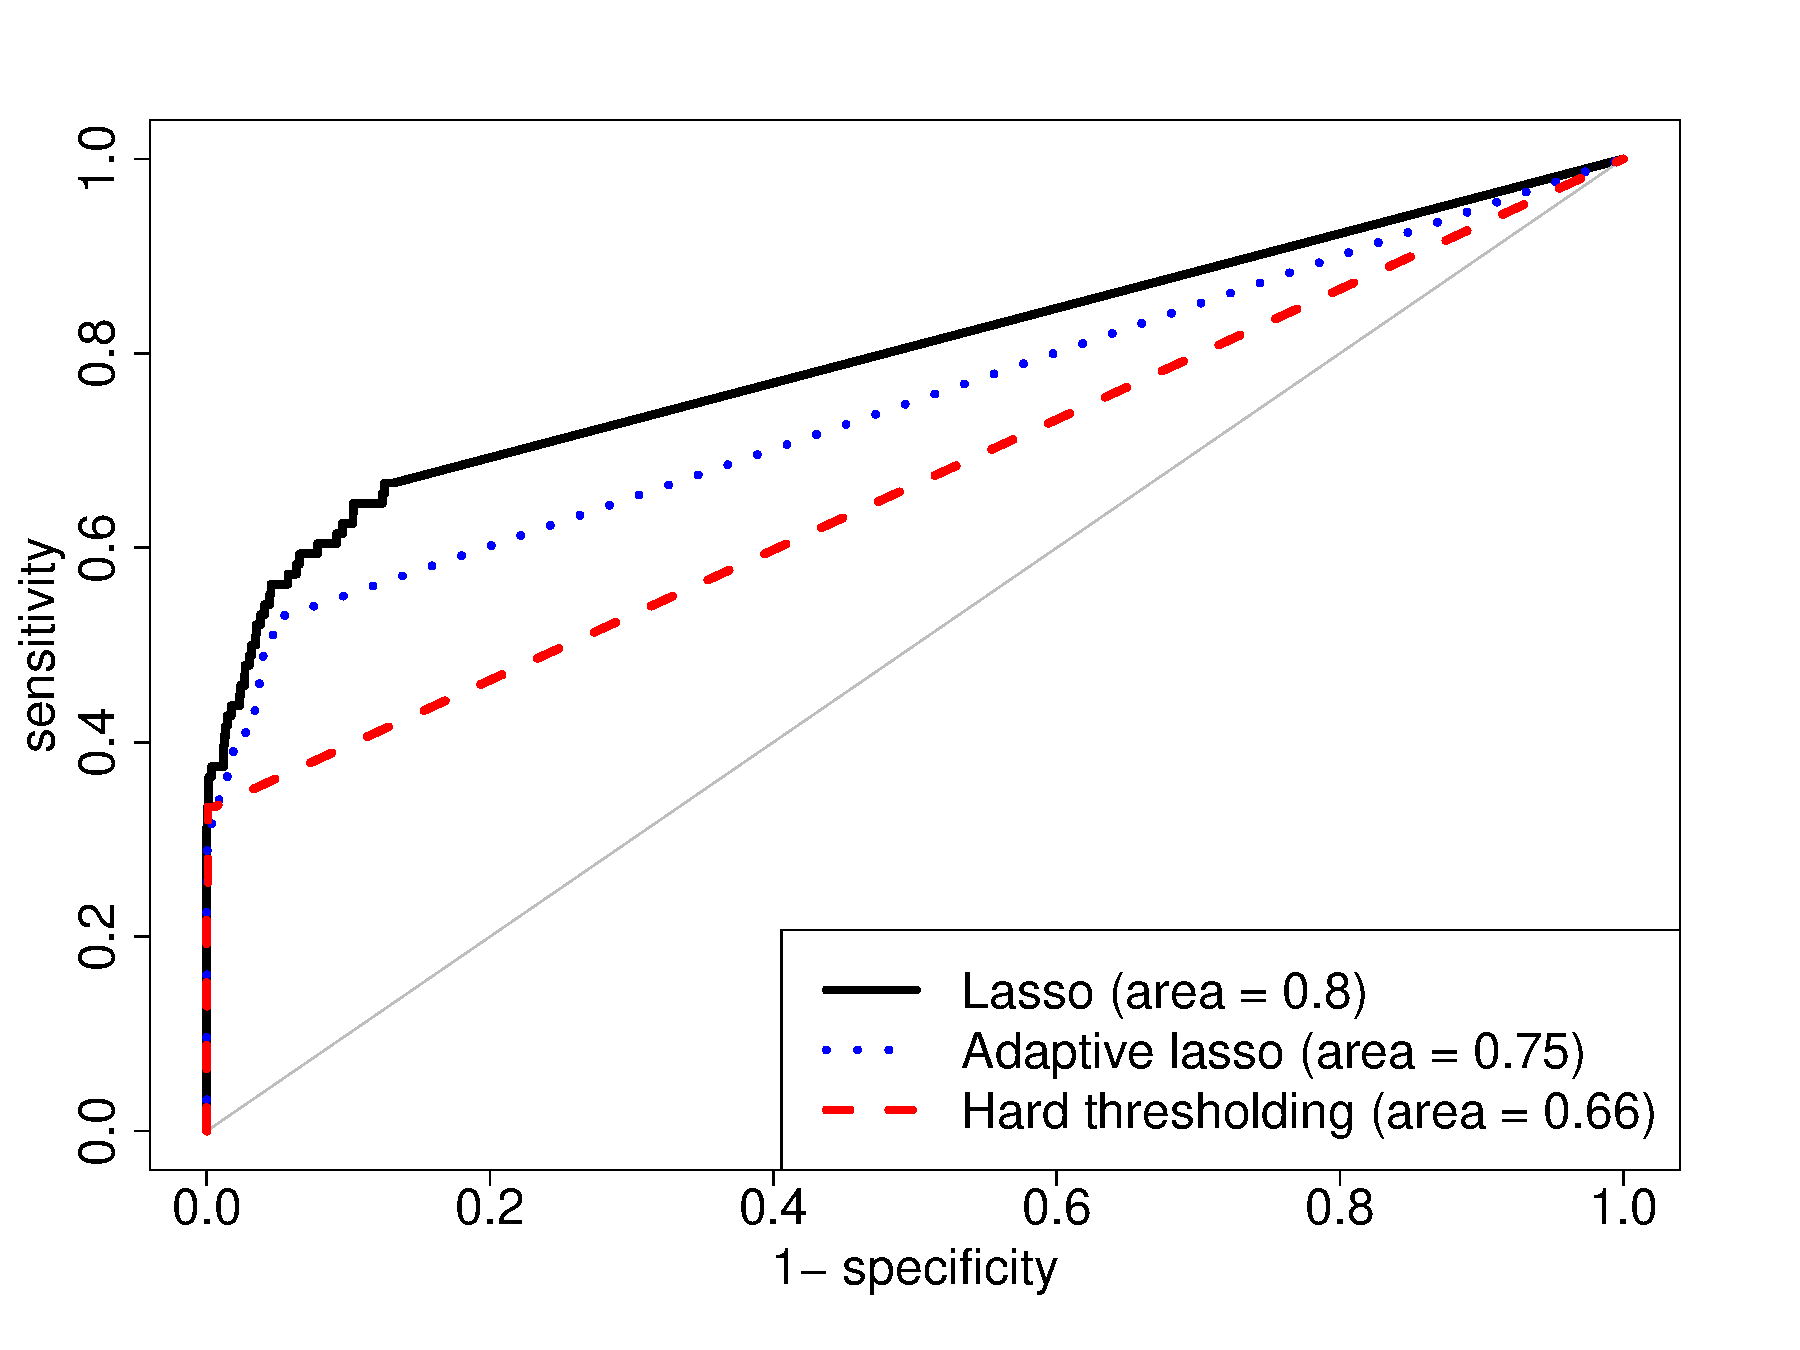
\includegraphics[width=0.48\textwidth]{img/ROC_100_96.pdf}
    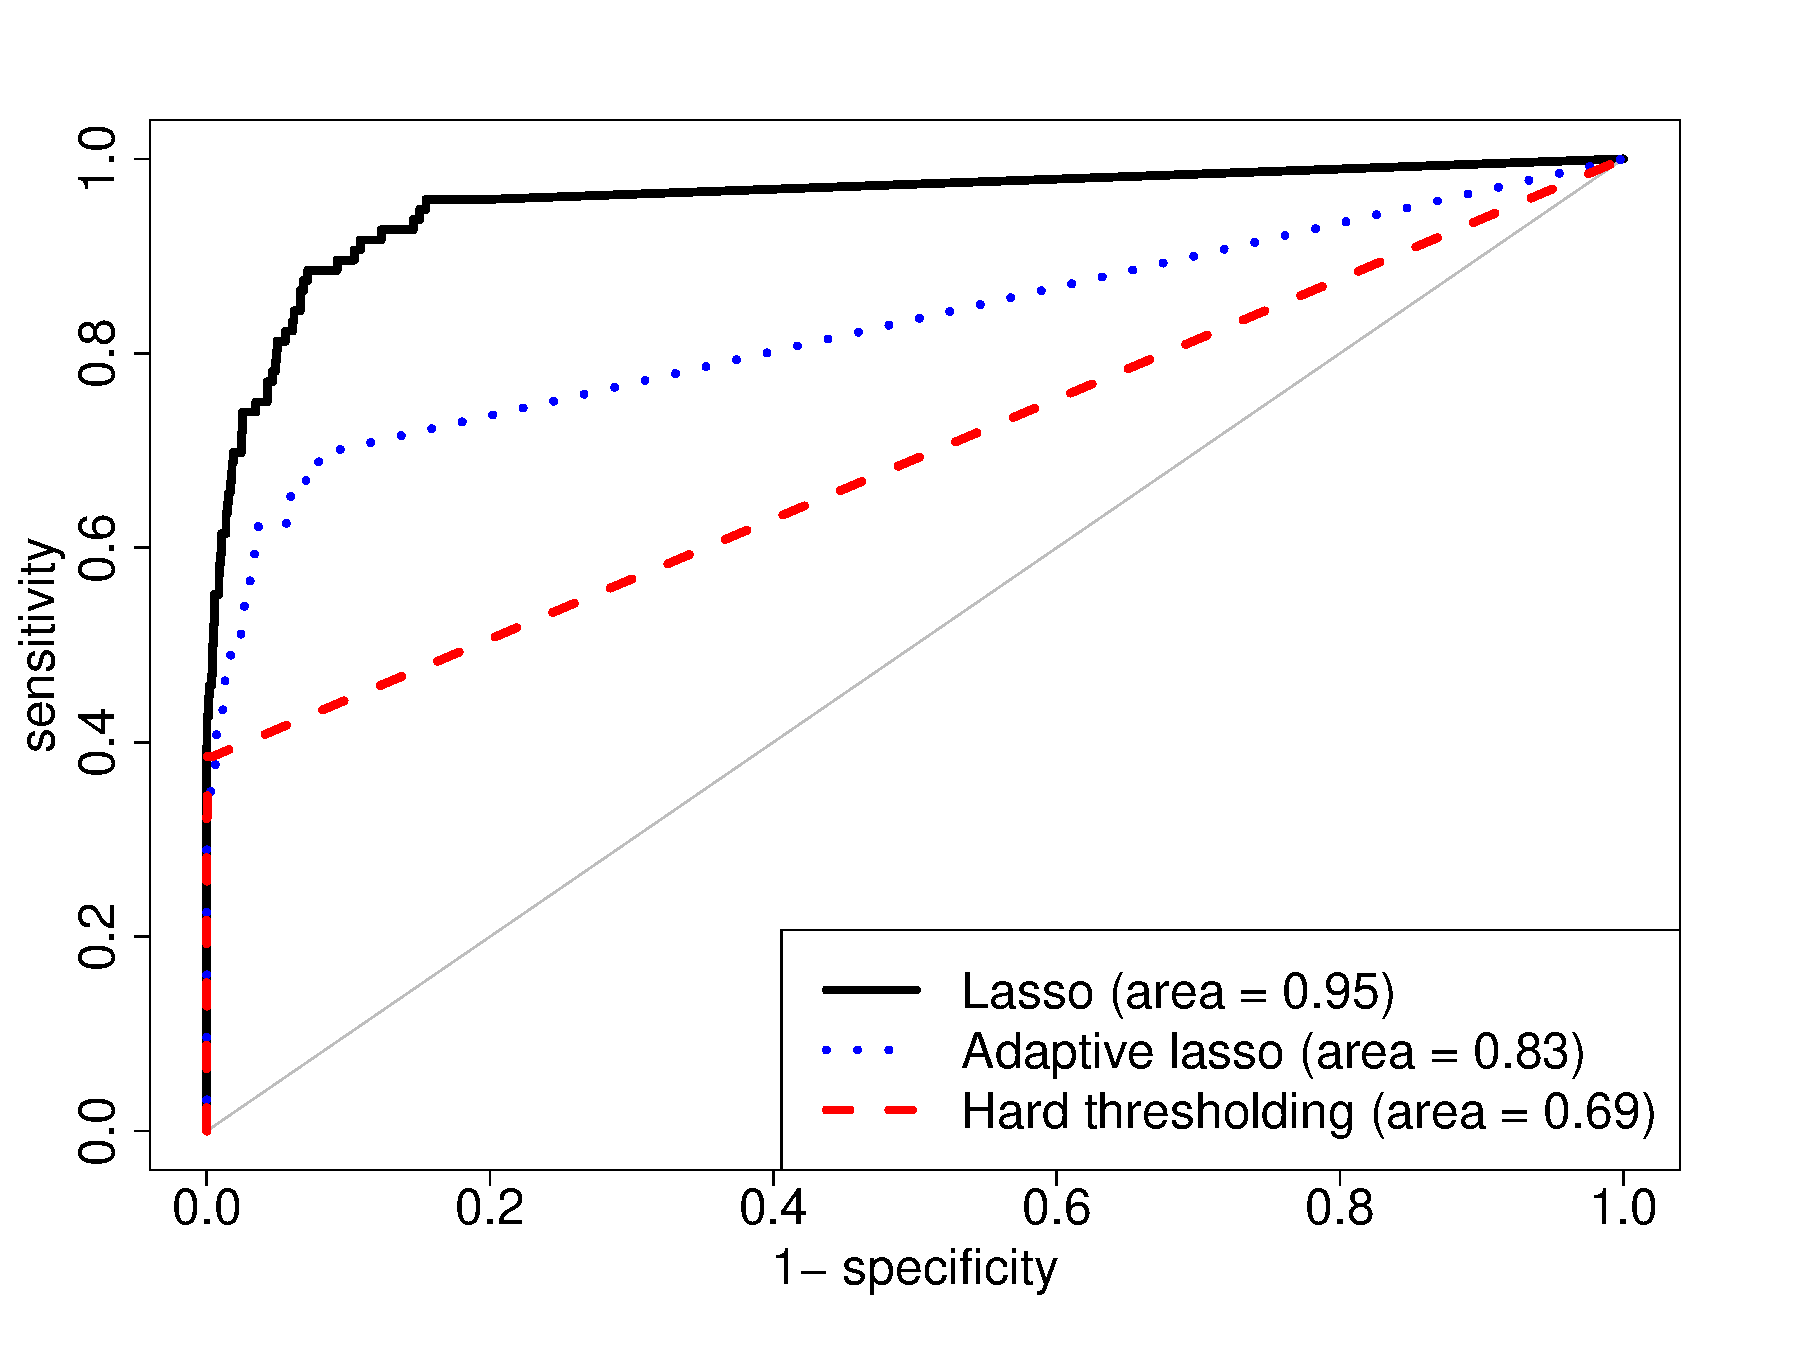
\includegraphics[width=0.48\textwidth]{img/ROC_200_96.pdf}
    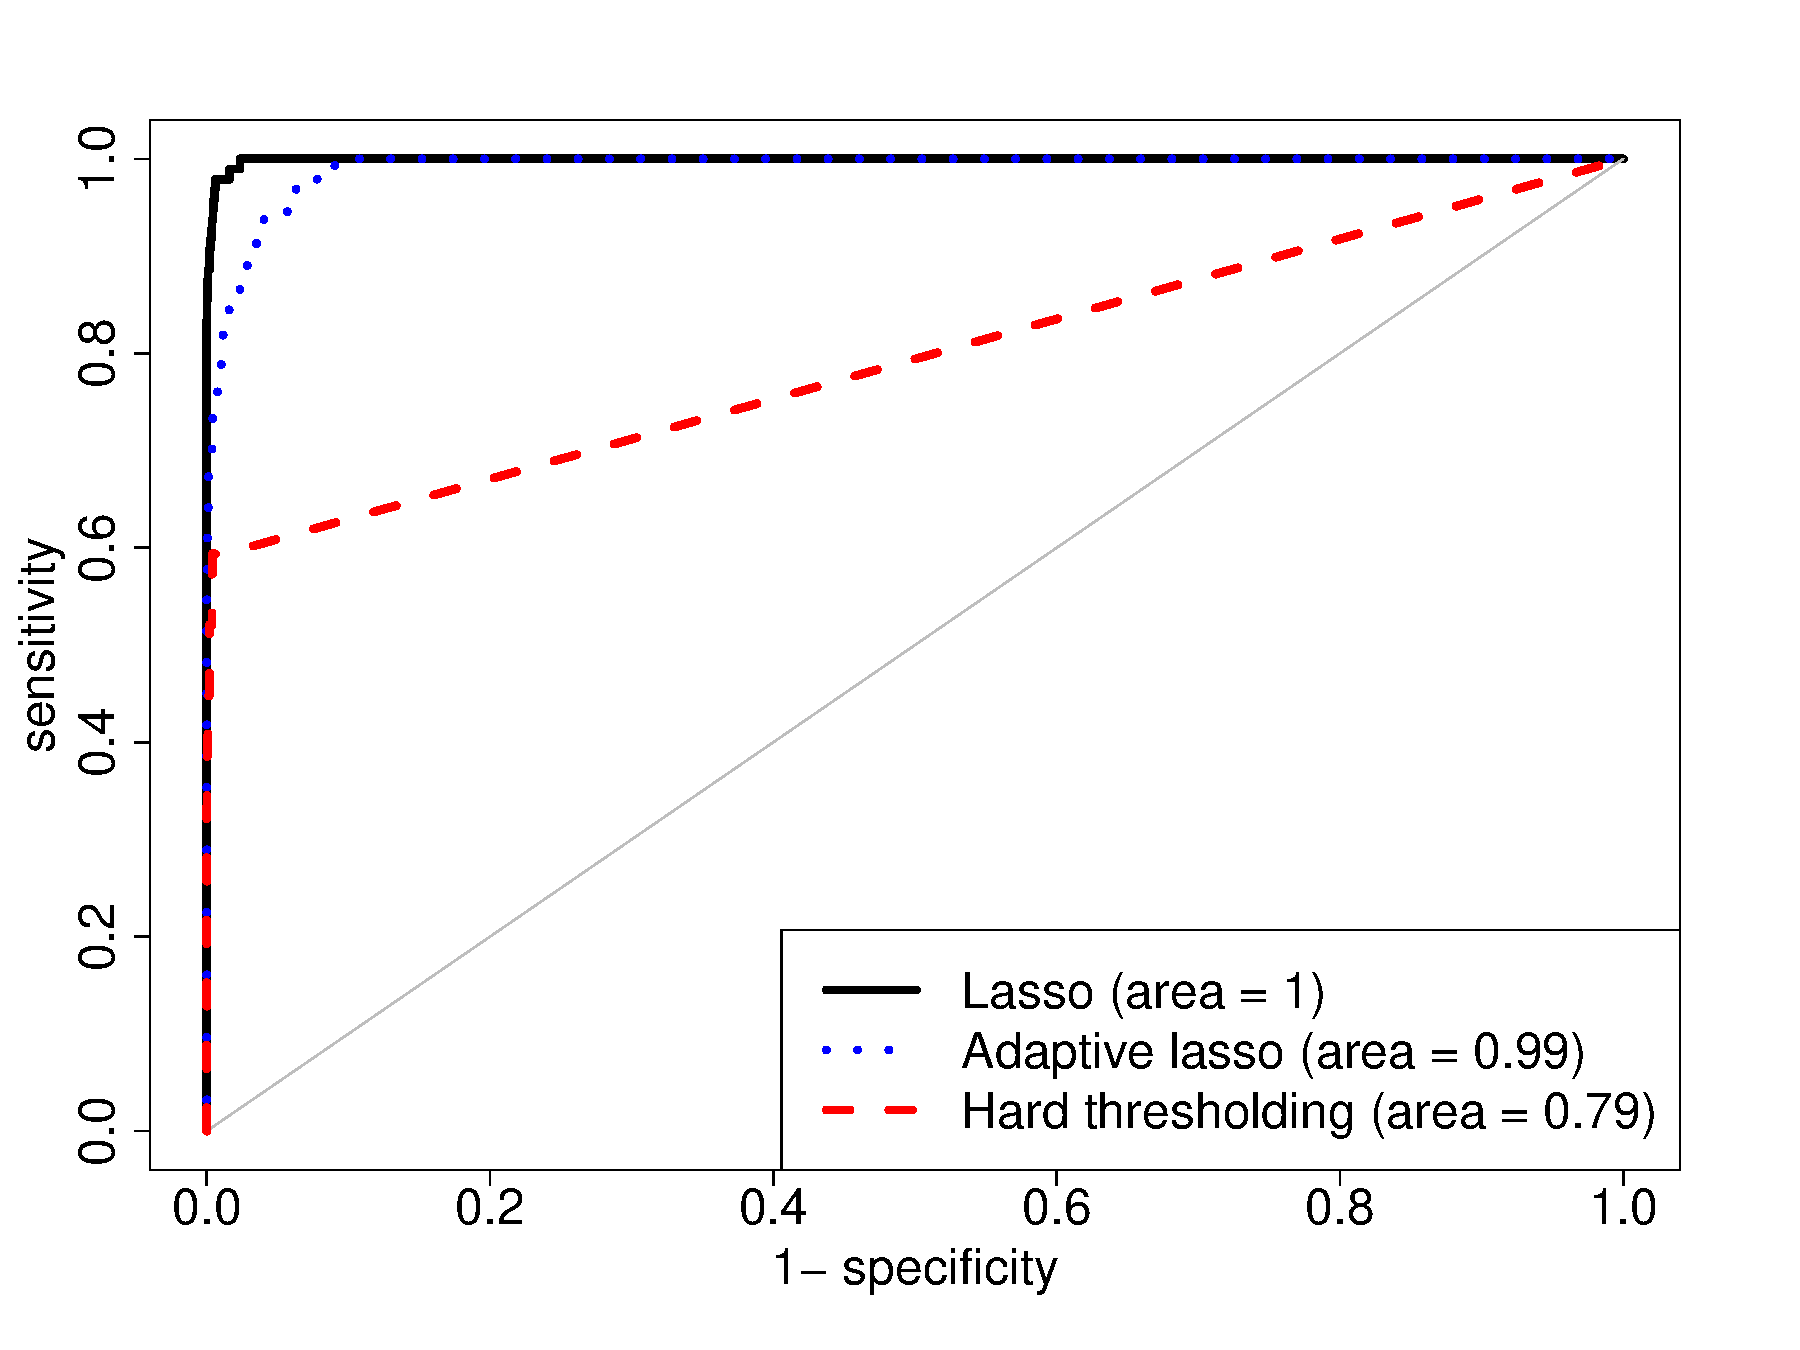
\includegraphics[width=0.48\textwidth]{img/ROC_400_96.pdf} 
    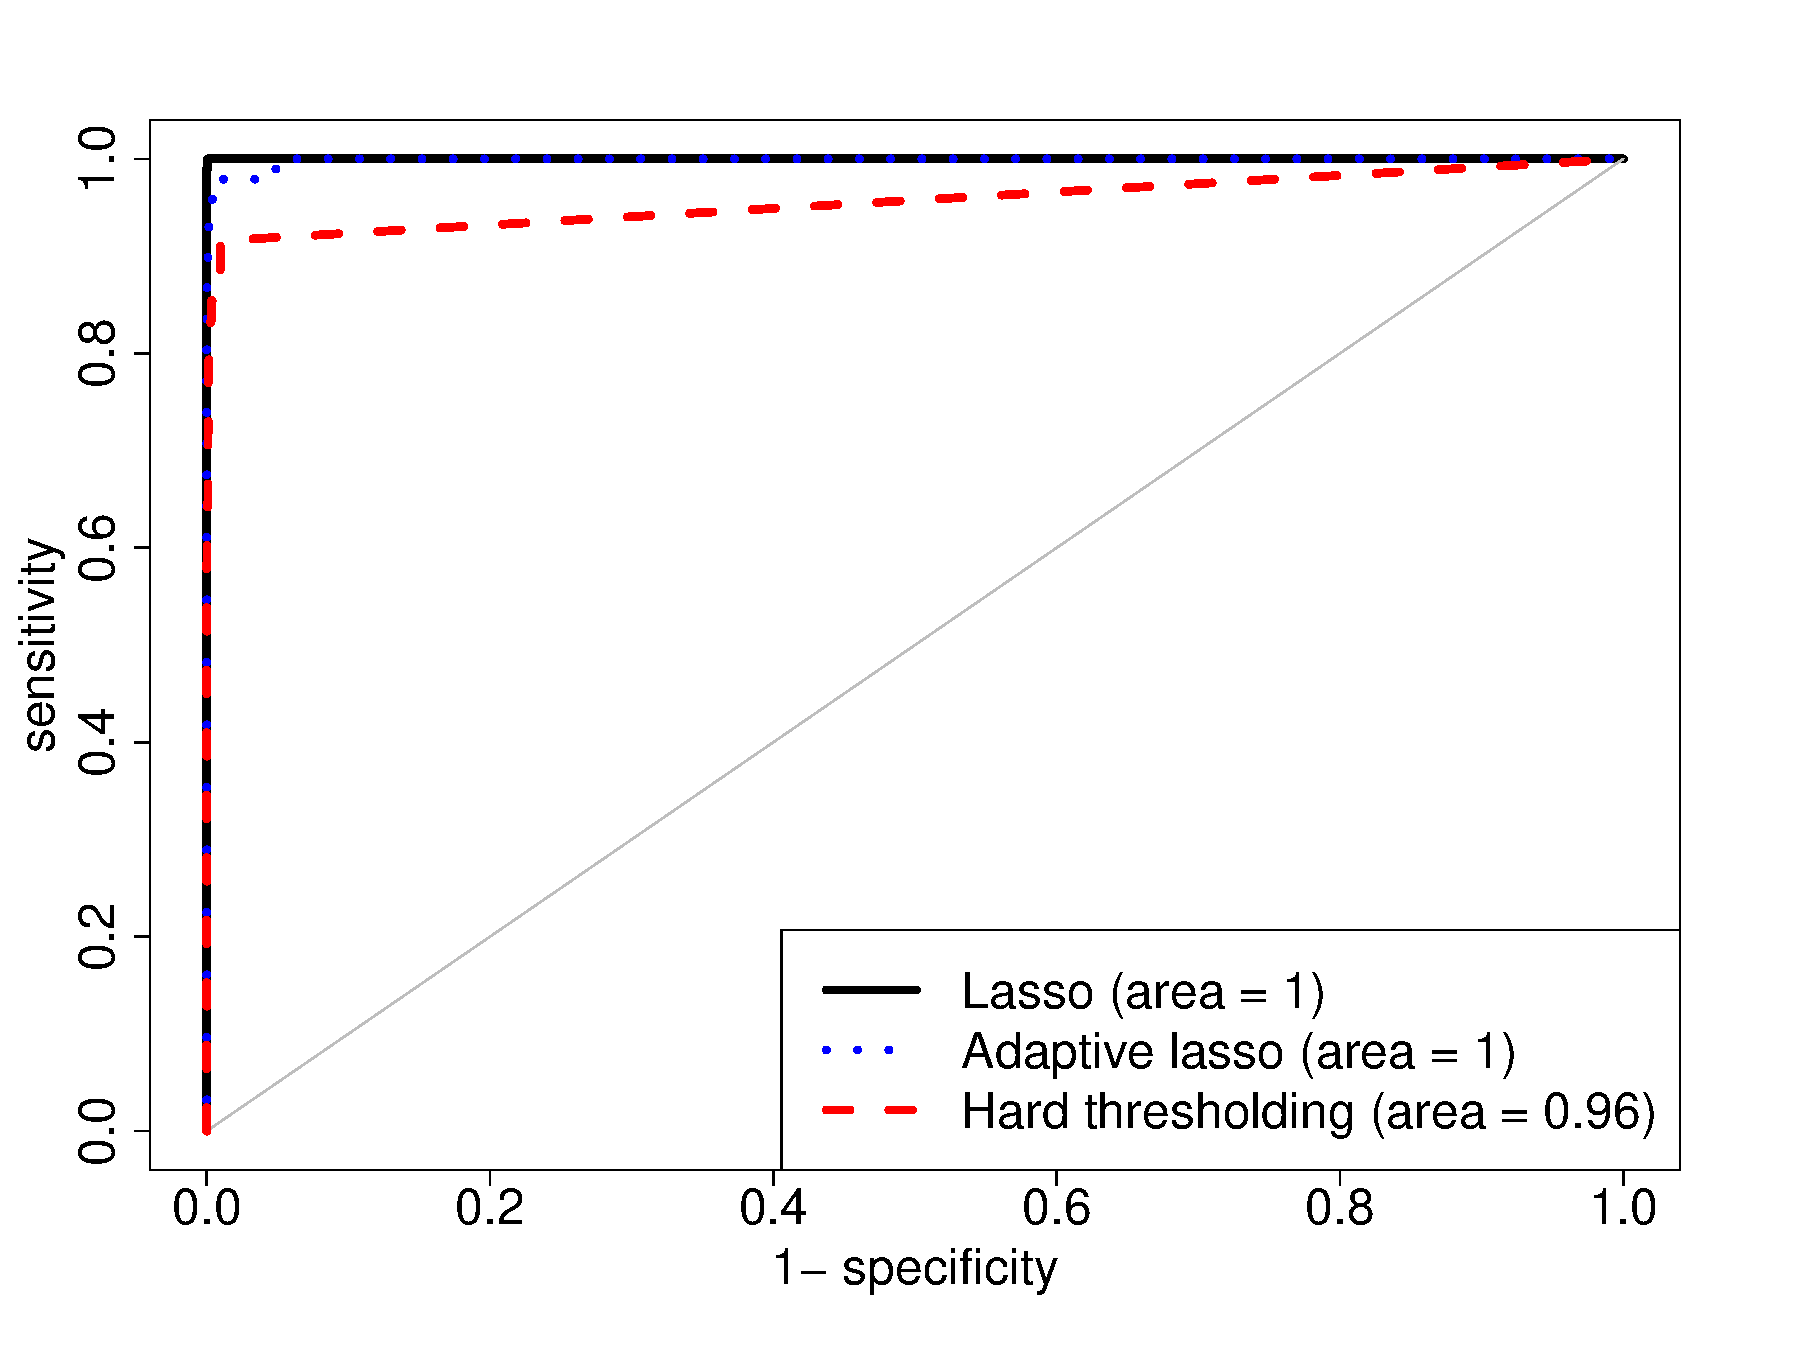
\includegraphics[width=0.48\textwidth]{img/ROC_600_96.pdf}    
    \caption{Receiver Operating Characeristic (ROC) curves of hard thresholding, lasso and adaptive lasso for recovering coherence network of a $p = 96$ dimensional VAR(1) model using $n = 100$ (top left), $n = 200$ (top right), $n = 400$ (bottom left) and $n = 600$ (bottom right) time series observations.}
    \label{fig:roc}
\end{figure}


% The results for heterogeneous settings are reported in Tables \ref{table:rmise-heterogeneous} and \ref{table:precision-heterogeneous}. Compared to homogeneous setting, RMISE of the three thresholding based methods outperform shrinkage estimators by a larger margin. {\color{red} [Sumanta: add description of precision/recall, and Figure \ref{fig::hetero}]. }




%\subsection{Tables and Graphs}




\section{Functional Connectivity Analysis with fMRI Data}\label{sec:realdata}


We demonstrate the advantage of thresholding based spectral density estimators for visualization and interpretation in functional connectivity analysis among different brain regions of a human subject using resting state fMRI data. This data is part of a study involving 51 subjects (29.6 $\pm$ 8.6 years of age, 35 males) that suffered from mild traumatic brain injury (TBI). Magnetic resonance imaging (MRI) data and neuropsychological data were collected at 1 week, 1 month, 6 months and 12 months post-injury. TBI is defined as Glasgow Coma Scale of 13-15 at injury, loss of consciousness less than 30 minutes and post-traumatic amnesia less than 24 hours. More  details are available in  \cite{Kuceyeski2018functional}. 
%We focus on the MRI collected at 1 month and 6 month because most recovery in this cohort occurred between these two time points \citep{Kuceyeski2018functional}. 
% {\color{red} Here you can reference my bioRxiv paper from this year that shows most cognitive recovery occurred between 1 and 6 months in this dataset.}

%After removal of observations collected at 1 week and 12 months, the dataset is balanced but not complete. There were a total of 27 subjects (29.1 $\pm$ 8.1 years of age, 21 males) with both imaging and  neuro-psychological measurements at 1 and 6 months. The same MRI sequences for demographic matched controls (28.6 $\pm$ 8.8 years of age, 25 males) were also collected for comparison.

\begin{figure}
    \centering
    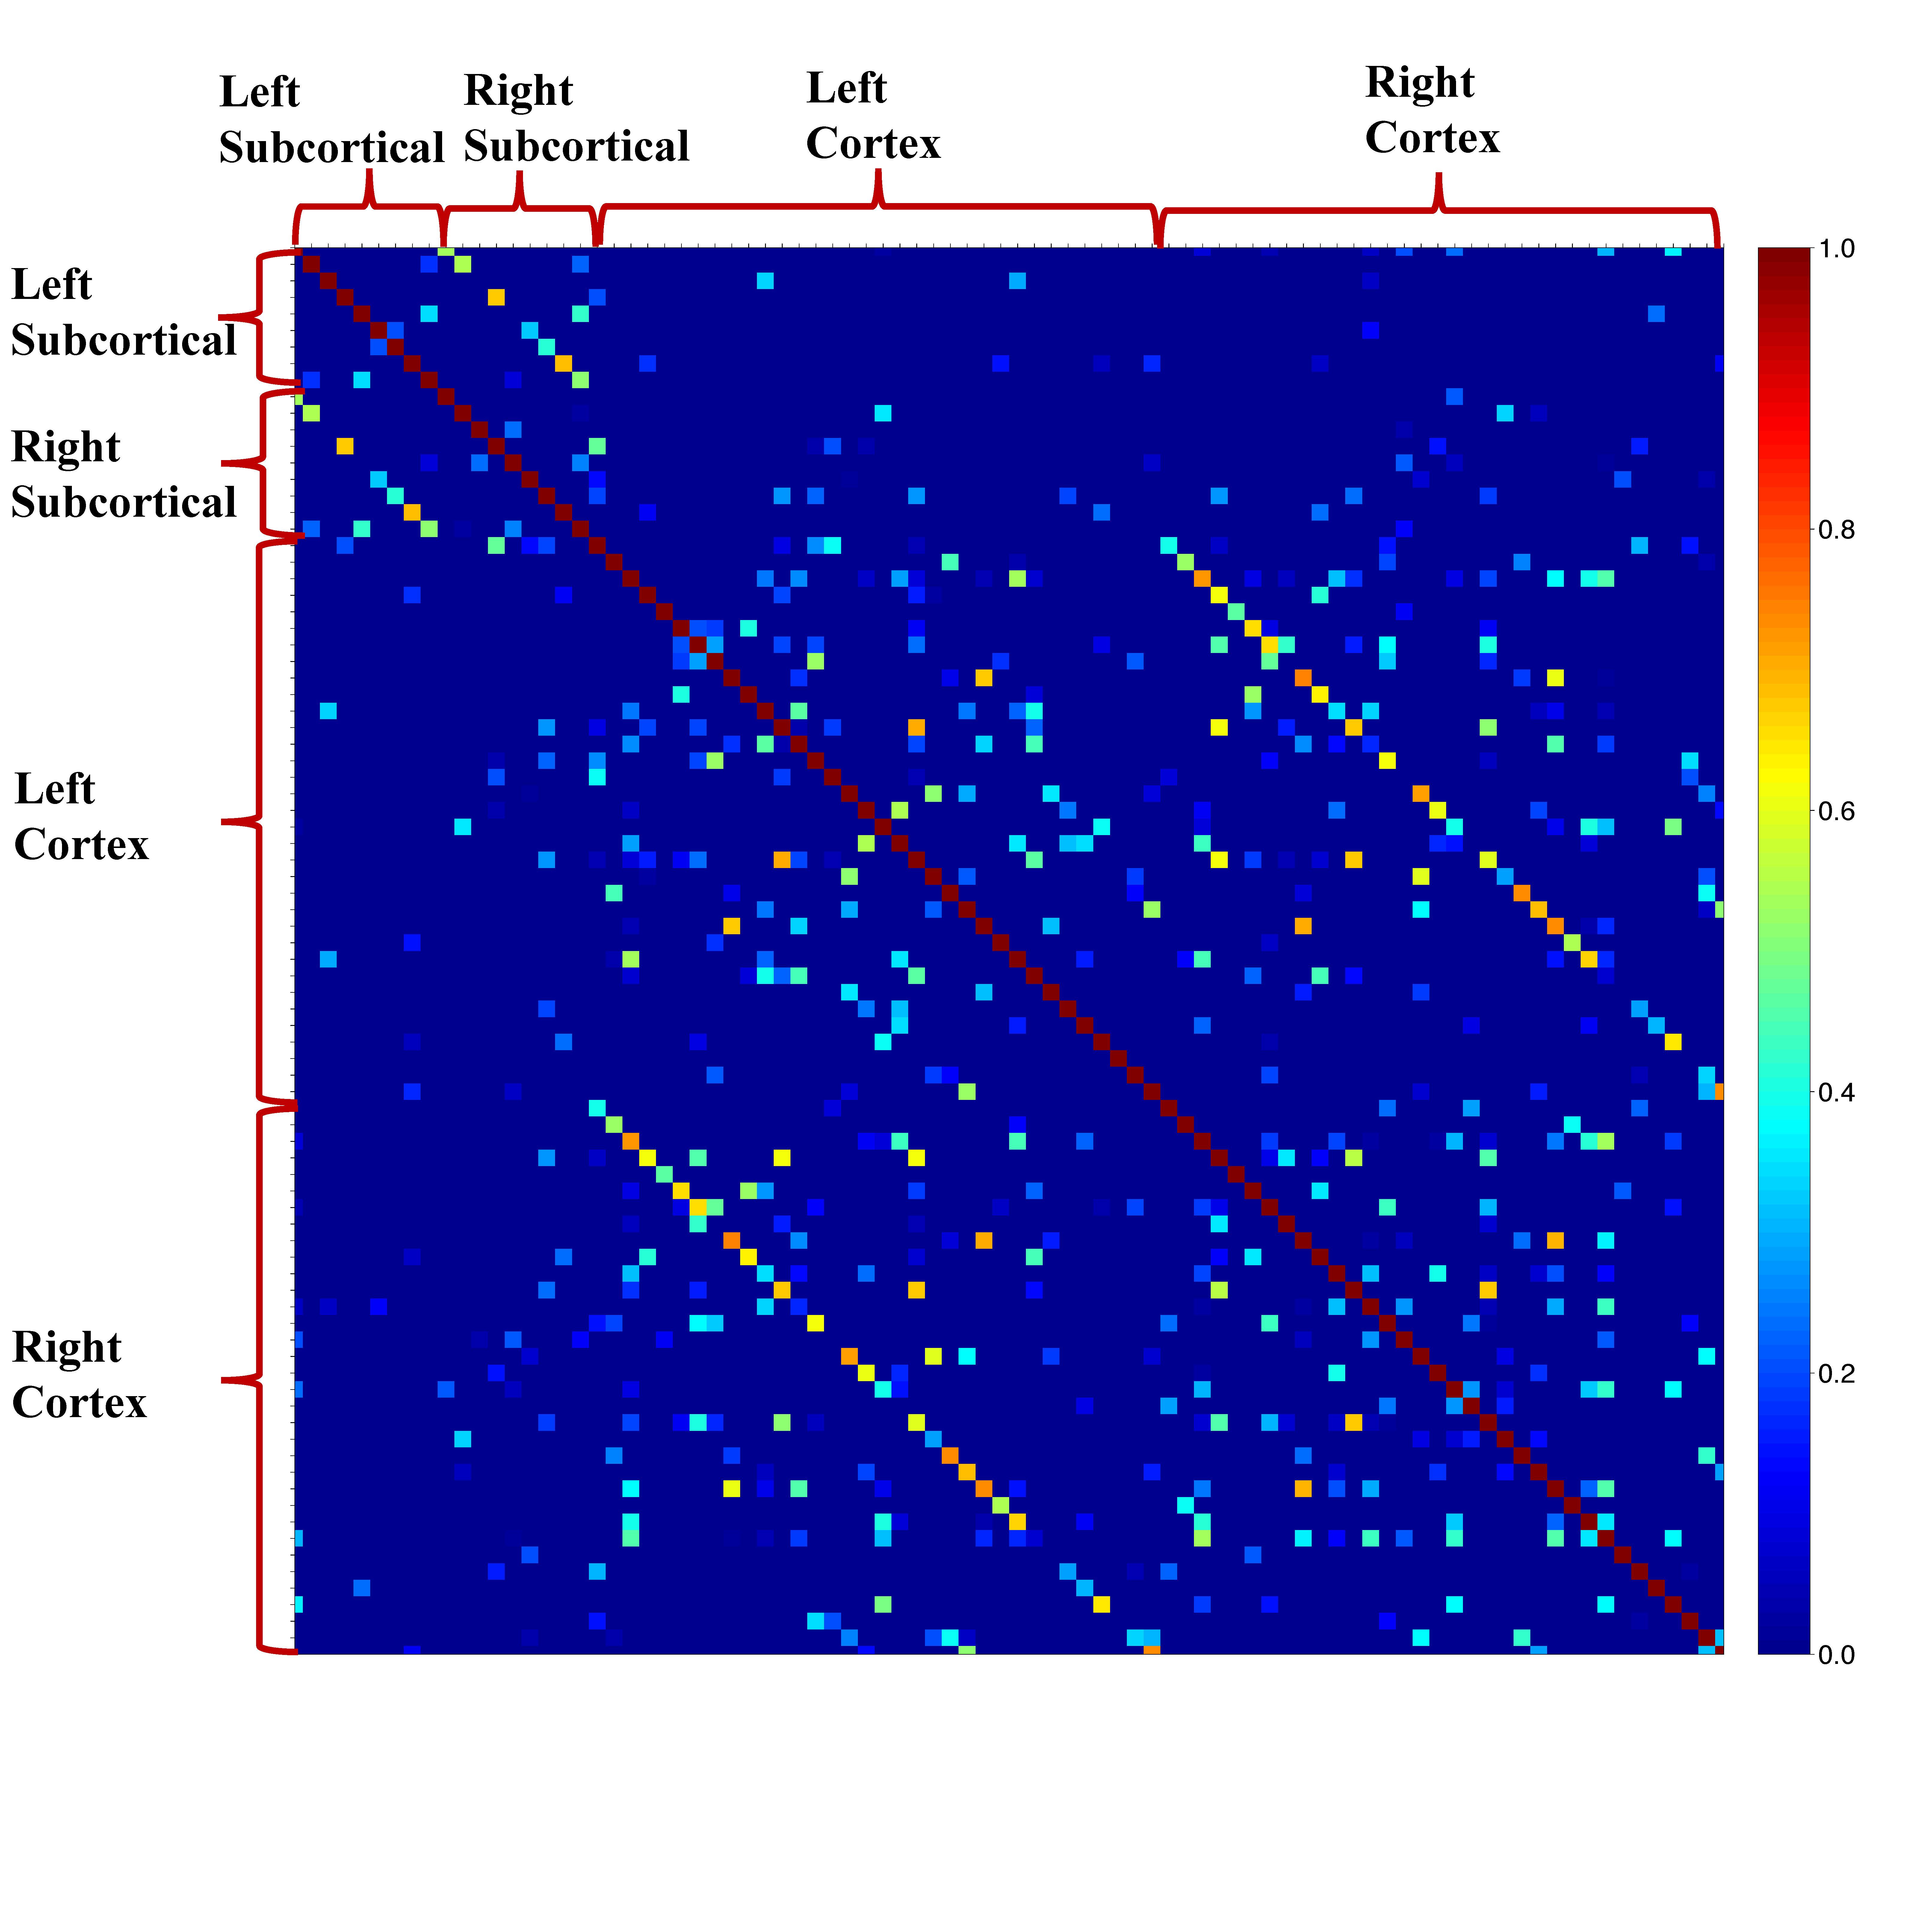
\includegraphics[width=0.48\textwidth]{img/al_hm_nl.pdf}
    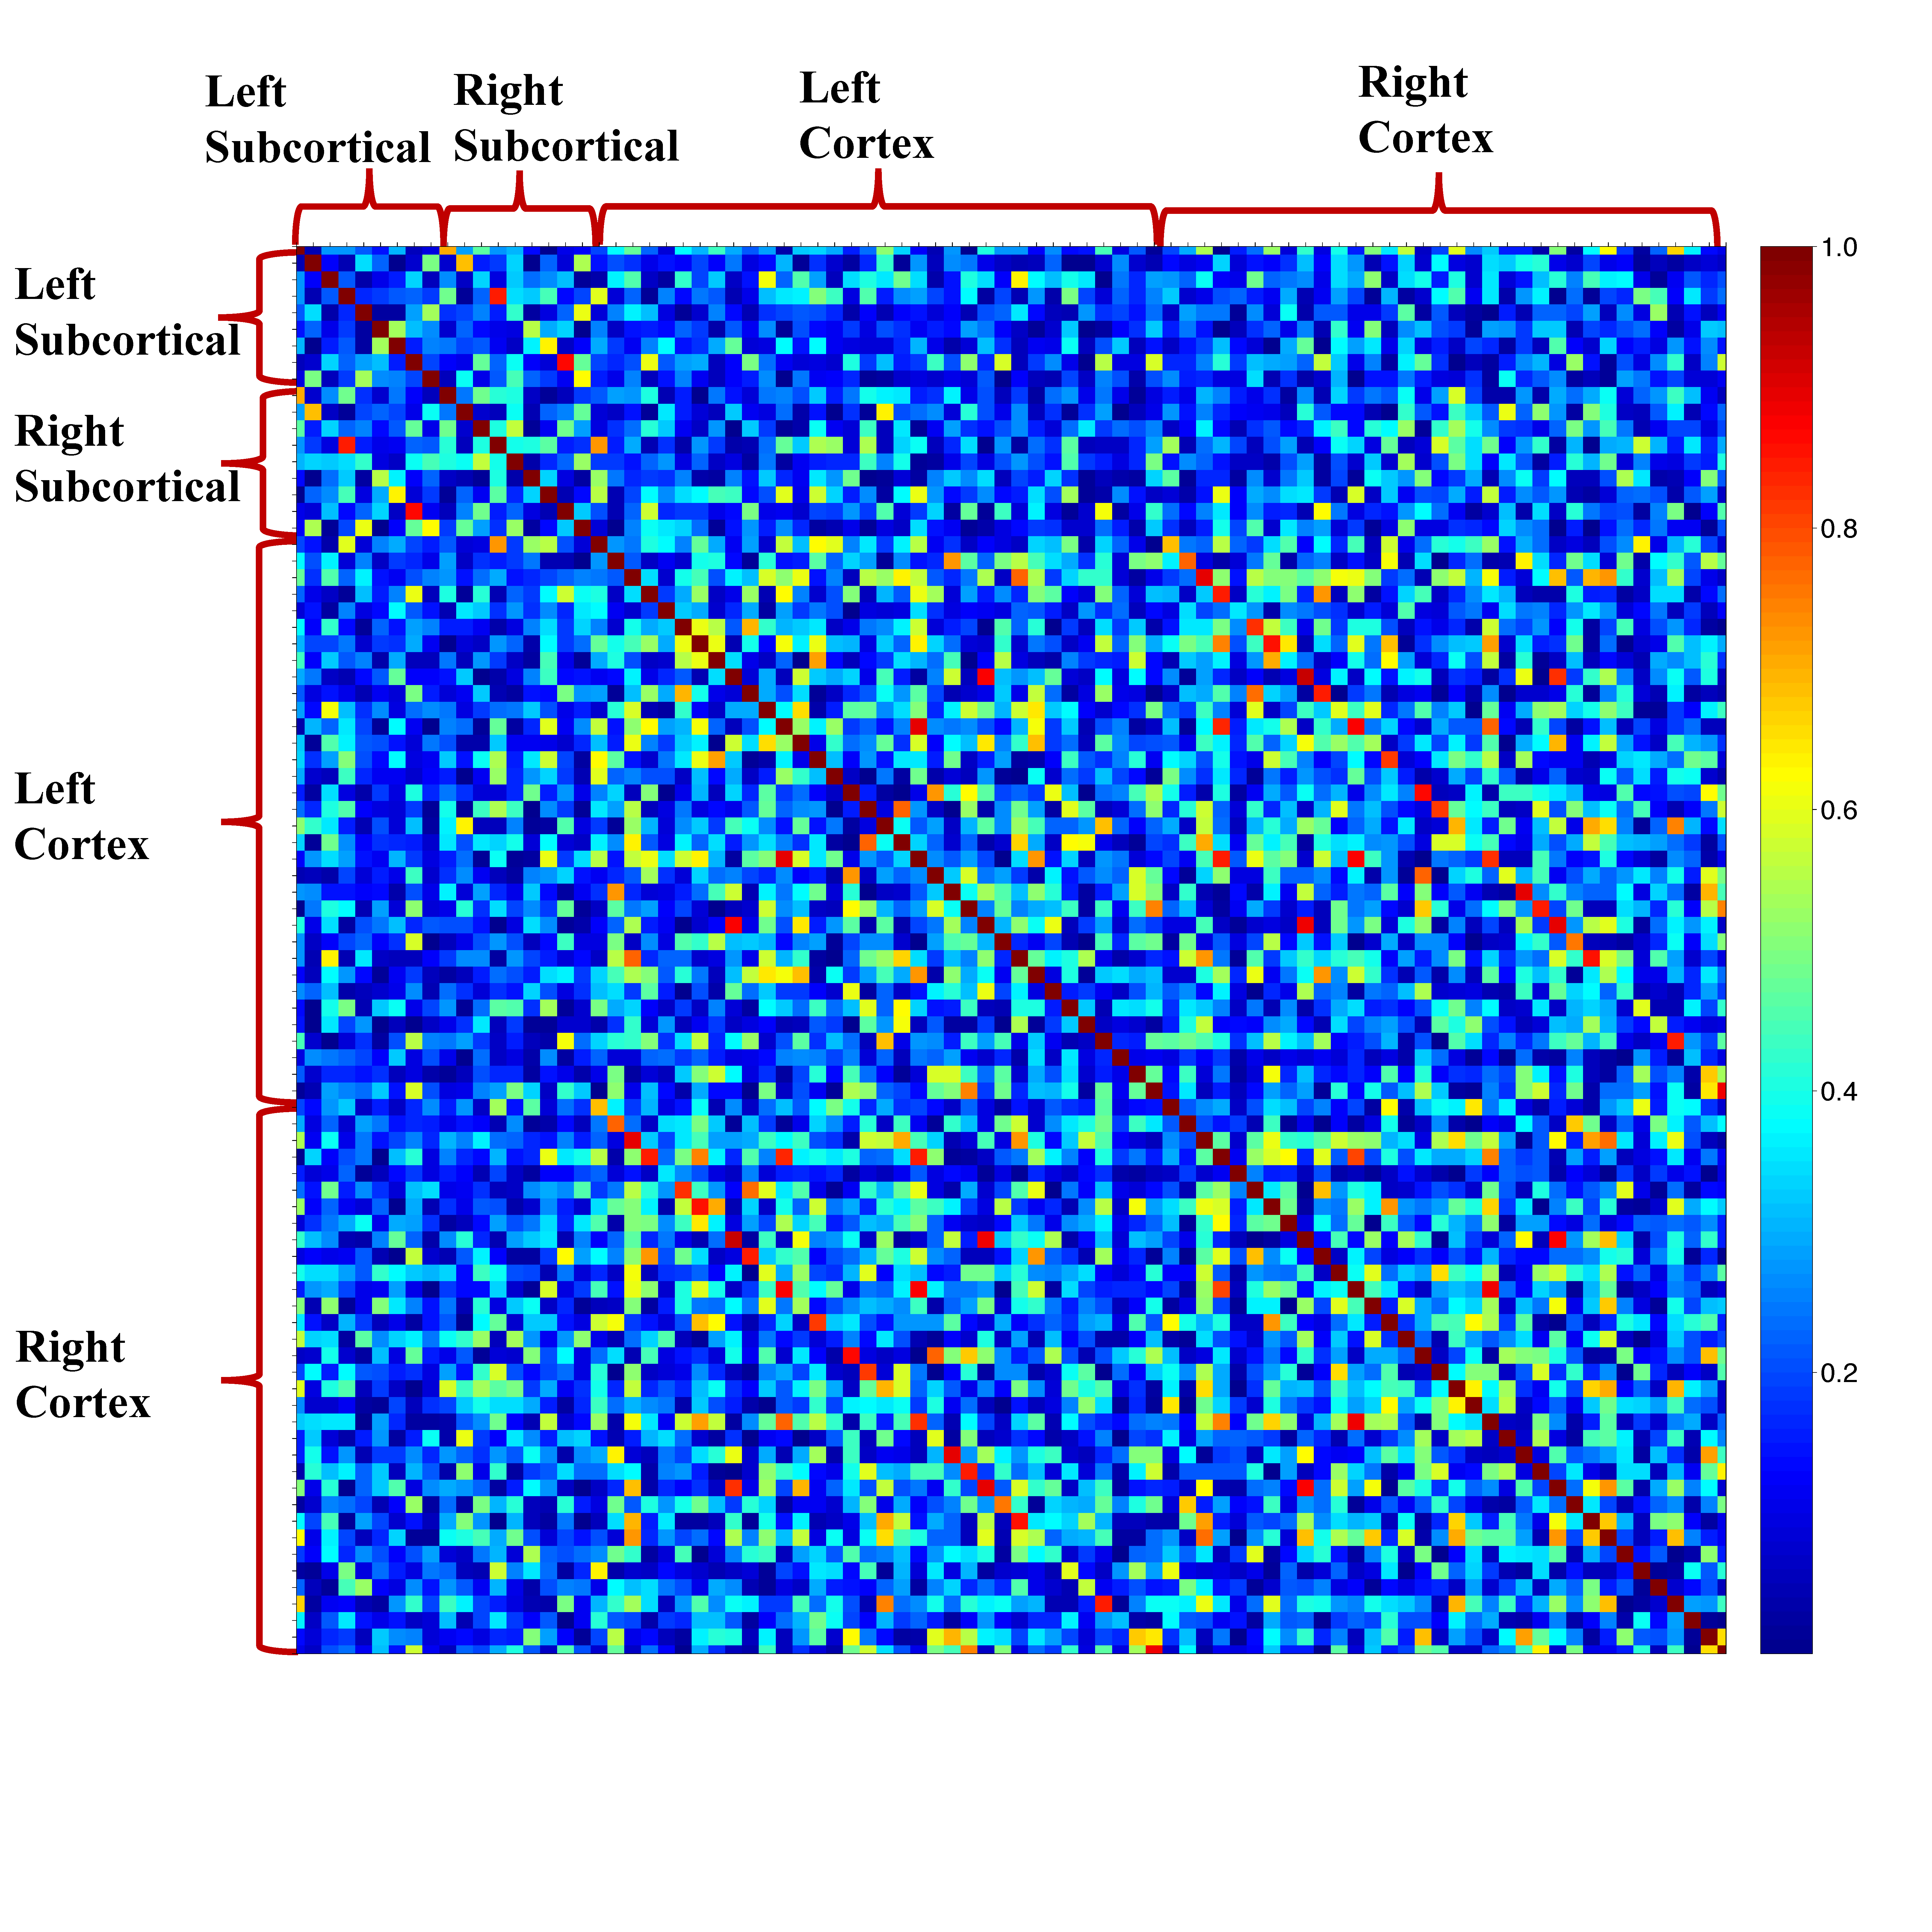
\includegraphics[width=0.48\textwidth]{img/sh_hm_nl.pdf}
    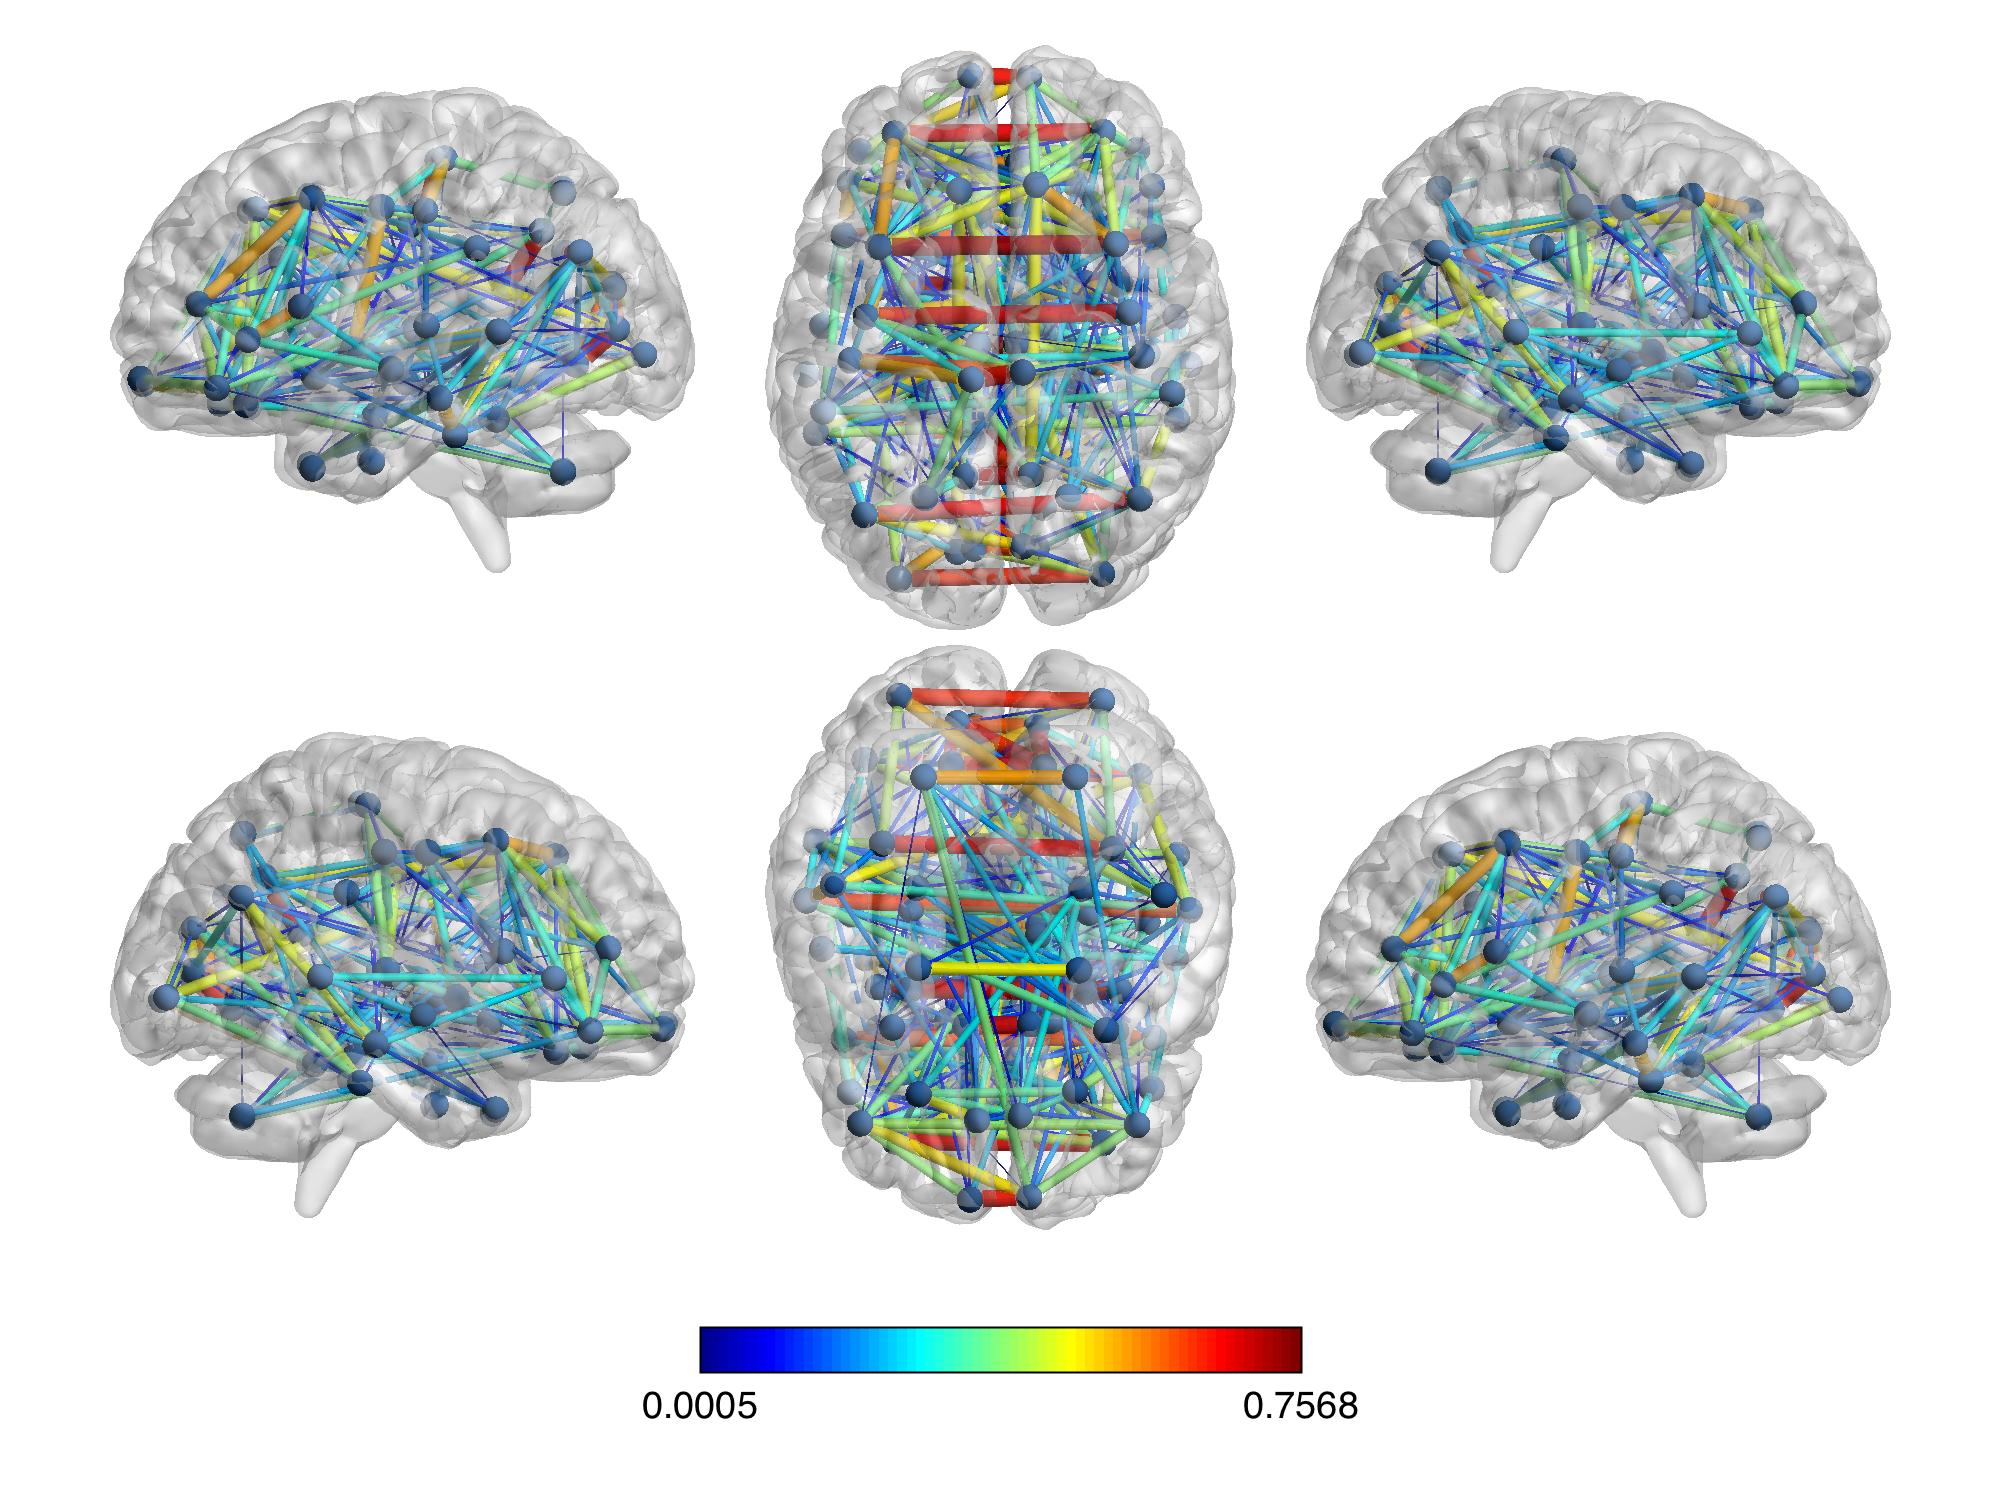
\includegraphics[width=0.95\textwidth]{img/al_c.jpg}
    \caption{[top]: Heat maps of absolute coherence matrices (at frequency $0$) obtained from  spectral density estimated using [top left] adaptive lasso thresholding  and [top right] a shrinkage method. [bottom]: Absolute coherence network among brain regions obtained using adaptive lasso and visualized using BrainNet Viewer. The coherence network estimated by adaptive lasso retains known biological patterns, including presence of bilateral homologues, i.e. strong connectivity between same ROIs in the left and right parts of brain.}
    \label{fig:realdata}
\end{figure}


A 3T GE Signa EXCITE scanner was used to  acquire the MRIs, which included structural scans (FSPGR T1, $1\times 1 \times 1$ mm$^3$ voxels) and resting-state functional magnetic resonance imaging (fMRI) (7 min, $3.4 \times 3.4 \times 4.0$ mm$^3$ voxels, 2 sec sampling rate). The MRIs were processed by parcellating the gray matter into $p=86$ anatomical regions of interest (ROIs) using the semi-automated FreeSurfer software \citep{fischl2000measuring}. Cortical and subcortical parcellations and the fMRI time series data were then used in the construction of coherence based functional connectivity (FC) networks. The adjacency matrix of FC network captures the similarity of the neuronal activation over time between pairs of ROIs. 

We calculated coherence matrices at frequency $0$ using adaptive lasso thresholding (with $\eta = 2$) and shrinkage of averaged periodograms. The smoothing span was chosen by setting $m=\sqrt{n}$, and the tuning parameters in our sample-splitting algorithm were selected as in our simulation studies. 

\textit{Results}: In Figure \ref{fig:realdata}, we show an example of the FC coherence network for a particular TBI patient using our proposed adaptive lasso thresholding (top left) and the same patient's FC network estimated using the shrinkage method (top right) of \cite{bohm2009shrinkage} that does not perform automatic coherence selection. One of the many issues with using fMRI data is the spurious functional connections that arise from the method's abundant noise (due to instrumentation and physiology). It is often preferable in a clinical context to filter out this noise, but it is not currently done in a universally accepted and statistically principled way. As shown in the top panel of Figure \ref{fig:realdata}, the coherence matrix estimated by adaptive lasso thresholding obviously is more sparse in nature compared to the one from shrinkage method, while maintaining known physiological connections. For example, we see strong FC in the bilateral homologues (the same ROI in the left versus right hemisphere), which are known to have strong functional connections \citep{zuo2010growing}. This is even more readily apparent in the bottom panel of Figure \ref{fig:realdata} where we see strong connections between the same ROI in the left and right sides of the brain. Other than the bilateral homologues, the left and right precuneus, isthmus cingulate, lingual gyrus and pericalcarine have prominent connections to many regions (see Figures \ref{fig:realdatafullalasso} and \ref{fig:realdatafullshrinkage} in Appendix \ref{appendix:more_tables}). The precuneus, which plays a role in visual, sensorimotor, and attentional information processing, is central to resting-state (task negative) fMRI networks detected using correlation analysis \citep{Utevsky14}. Additionally, the isthmus cingulate, part of the posterior cingulate cortex, is known to be highly functionally connected to many regions across the brain at rest \citep{FRANSSON20081178}. In addition, we see a stronger FC between the left and right homologues in the subcortical ROIs (upper left corner) than between subcortical and cortical ROIs. It is interesting to note that while some of these connections are also strong in the shrinkage based coherence matrix estimate, it is not easy to separate them from other moderately strong coherences between brain regions.




\section{Discussion}\label{sec:discussion}
We proposed hard thresholding and generalized thresholding of averaged periodogram for estimation of high-dimensional spectral density matrices of stable Gaussian time series and linear processes with errors having potentially heavier tails than Gaussian. Under high-dimensional regime $\log p /n \rightarrow 0$, we established consistency of the above estimation procedures when the true spectral densities are weakly sparse. At the core of our technical results lie concentration inequalities of  complex quadratic forms of temporally dependent, high-dimensional random vectors, which were used to derive finite sample deviation of averaged periodograms around their expectation. These results  are of independent interest and are potentially useful in other problems involving high-dimensional spectral density. In our next steps, we plan to extend the theoretical analyses to more general adaptive thresholding methods \citep{cai2011adaptive}, which will explicitly account for heterogeneity in the strengths of cross-spectral association across different pairs of time series and different frequency bands. We also plan to develop estimation and inference procedures for high-dimensional partial coherence at different frequencies.

Another direction of potential interest is to develop thresholding strategies that incorporate  information on different brain regions and prior biological knowledge on brain networks. Dynamic functional connectivity of brain networks is known to play important roles behind progression of neurodegenerative diseases. A common approach to build such networks is using coherence measures of Fourier or wavelet transform of multi-channel fMRI/EEG/MEG signals and thresholding small entries of zero. Selection of threshold level that represents heterogeneous modular structure of human brain has been a topic of active research \citep{bordier2017graph}. We expect that more sophisticated thresholding methods, building up on universal and adaptive thresholds and incorporating prior neuroscientific knowledge, will be potentially useful in  data-driven discovery of scientifically and clinically relevant connectivity patterns in human brain.

\clearpage
\begin{subappendices}
\section{Appendix: Proofs for Gaussian Time Series}\label{appendix:proof_gaussian}
\subsection{Proof of Lemma \ref{lemma: hason_bound_time_gauss}}
\begin{proof}
We can write $vec(\mathcal{\mathcal{X}}^\top)\stackrel{d}{=}\Sigma^{1/2}Z$, where $\Sigma$ is the covariance matrix of the $np$-dimensional random vector $vec(\mathcal{\mathcal{X}}^\top)$ and $Z\sim N(0,I)$. Then using Hanson-Wright inequality [Theorem 1.1,  \cite{rudelson2013hanson}] and the fact that the subGaussian norm of $Z$ is $1$, we conclude that there exists a universal constant $c>0$ satisfying 
\begin{equation}
\label{eq: hanson1}
\begin{aligned}
&\mathbb{P}\left(\left|vec(\mathcal{\mathcal{X}}^\top)^\top A ~vec(\mathcal{\mathcal{X}}^\top) - \mathbb{E} \left[vec(\mathcal{\mathcal{X}}^\top)^\top A~ vec(\mathcal{\mathcal{X}}^\top)~\right]\right| >2\pi\eta\vertiii{f}\right) \\
&= \mathbb{P}\left(\left|Z^\top \Sigma^{1/2}A\Sigma^{1/2}Z - \mathbb{E}\left[ Z^\top \Sigma^{1/2}A\Sigma^{1/2}Z \right]\right|>2\pi \eta\vertiii{f}\right)\\
&\le 2\exp\left[-c\min\left\{\cfrac{2\pi \eta\vertiii{f}}{\|\Sigma^{1/2}A\Sigma^{1/2}\|},\cfrac{4\pi^2\eta^2\vertiii{f}^2}{\|\Sigma^{1/2}A\Sigma^{1/2}\|_F^2}\right\}\right].
\end{aligned}
\end{equation}




Using Lemma \ref{lemma:max-L2-norm}, $\|\Sigma^{1/2}A\Sigma^{1/2}\|\le \|\Sigma\|\|A\|\le 2\pi \vertiii{f} \|A\|$. It follows from \citet{golub2012matrix},
\begin{equation}
\begin{aligned}
&\|\Sigma^{1/2}A\Sigma^{1/2}\|_F \le \sqrt{\rank(\Sigma^{1/2}A\Sigma^{1/2})} \|\Sigma^{1/2}A\Sigma^{1/2}\| \nonumber \\
&\le \sqrt{\rank(A)} \|\Sigma^{1/2}A\Sigma^{1/2}\| \le 2\pi \sqrt{\rank(A)} \|A\| \vertiii{f}. \nonumber
\end{aligned}
\end{equation}
Then plugging in the bound for $\|\Sigma^{1/2}A\Sigma^{1/2}\|$ and 
$\|\Sigma^{1/2}A\Sigma^{1/2}\|_F$ into \eqref{eq: hanson1} completes the proof.
\end{proof}

\subsection{Proof of Proposition \ref{prop:bias_bound}}
\begin{proof}
It suffices to show that for any two unit vectors $e_r,e_s$, 
\begin{equation}
\begin{aligned}
\left|e_r^\top \left[\mathbb{E}\hat{f}(\omega_j) - f(\omega_j)\right]e_s\right| \le \frac{m}{n}\Omega_n(f) + \frac{1}{2\pi}\left(\frac{\Omega_n(f)}{n}+L_n(f)\right). \nonumber
\end{aligned}
\end{equation}
Since  
\begin{equation}
\hat{f}(\omega_j) = \frac{1}{2\pi(2m+1)} \sum_{\ell =-m}^m I(\omega_{j+\ell}),  \nonumber
\end{equation}
we have 
\begin{equation}
\label{eq:mul_dev}
\begin{aligned}
\left|e_r^\top \left[\mathbb{E}\hat{f}(\omega_j) - f(\omega_j)\right]e_s\right| 
&\le \frac{1}{2\pi(2m+1)} \sum_{\ell = -m}^m |e_r^\top\left[\mathbb{E}I(\omega_{j+\ell}) - \mathbb{E} I(\omega_{j})\right]e_s|\\
&+\left|e_r^\top \left[\frac{1}{2\pi}\mathbb{E}I(\omega_j) - f(\omega_j)\right]e_s\right|. 
\end{aligned}
\end{equation}
By definition of $I(\omega_j)$ in \eqref{eq:single_periodogram}, we have $\mathbb{E} I(\omega_j) = \sum_{|k| \le n} \Gamma(k) \frac{(n-|k|)}{n} e^{-ik \omega_j}$.  Therefore, the second term above takes the form 
\begin{equation}
\label{eq:mul_dev1}
\begin{aligned}
\left|\frac{1}{2\pi} e_r^\top \left[\mathbb{E} I(\omega_j) - 2\pi f(\omega_j)\right]e_s\right| &= \frac{1}{2\pi}\left|\sum_{|k|\le n} \frac{|k|}{n}  \Gamma_{rs}(k) e^{-ik\omega_j}+\sum_{|k|>n} \Gamma_{rs}(k) e^{-ik\omega_j}\right|\\
&\le \frac{1}{2\pi} \left [\sum_{|k|\le n} \frac{|k|}{n}  |\Gamma_{rs}(k)|+ \sum_{|k|>n} |\Gamma_{rs}(k)|\right]\\
&= \frac{1}{2\pi}\left(\frac{\Omega_n(f)}{n} + L_n(f)\right). 
\end{aligned}
\end{equation}
For the first term, note that $|e^{ix} - e^{iy}|\le |x-y|$ and $|\omega_j-\omega_{j+\ell}| = 2\pi \frac{|\ell|}{n}$. This implies 
\begin{equation}
\label{eq:mul_dev2}
\begin{aligned}
\left|\frac{1}{2\pi} e_r^\top \left[\mathbb{E} I(\omega_j) - \mathbb{E} I(\omega_{j+\ell}) \right]e_s\right| &= \frac{1}{2\pi}\left|\sum_{|k|\le n} \left(1-\frac{|k|}{n}\right) |\Gamma_{rs}(k)| (e^{-ik\omega_j} - e^{-i k\omega_{j+\ell}})\right|\\
&\le \frac{1}{2\pi} \sum_{|k|\le n} |\Gamma_{rs}(k)| |k||\omega_j - \omega_{j+\ell}| =  |\ell| \Omega_n(f)/n. 
\end{aligned}
\end{equation}
Plugging in \eqref{eq:mul_dev1} and \eqref{eq:mul_dev2}  into \eqref{eq:mul_dev},  
\begin{equation*}
\begin{aligned}
\left|e_r^\top \left[\mathbb{E}\hat{f}(\omega_j) - f(\omega_j)\right]e_s\right| &\le \frac{1}{2\pi}\left(\frac{\Omega_n(f)}{n} + L_n(f)\right)+ \left(\frac{\sum_{|\ell|\le m} |\ell|}{2m+1}\right)\frac{\Omega_n(f)}{n}\\
&\le \frac{m}{n}\Omega_n(f) + \frac{1}{2\pi}\left(\frac{\Omega_n(f)}{n}+L_n(f)\right).\nonumber
\end{aligned}
\end{equation*}
\end{proof}


\subsection{Proof for Proposition \ref{prop:order_bias}}
\begin{proof}
We will prove the proposition one by one for its three conditions. Proof for all three conditions uses the simple fact that, for $0<x<1$
\begin{equation}
\label{eq:sum-help}
\sum_{\ell=1}^n \ell x^\ell = \frac{x(1+nx^{n+1}-(n+1)x^n)}{(1-x)^2}.
\end{equation}

\paragraph{Condition 1:} Directly plug the bound on $\|\Gamma(\ell)\|_{\text{max}}$ and with $|\Gamma_{r,s}(\ell)|\le \|\Gamma(\ell)\|_{max}$, we have 

\begin{equation}
\Omega_n \le 2 \sum_{\ell=1}^n \ell \|\Gamma(\ell)\|_{\text{max}}\le  2 \sigma_X \sum_{\ell=1}^n \ell \rho_X^{\ell} = \frac{2\sigma_X\rho_X (1+n\rho_X^{n+1}-(n+1)\rho_X^n)}{(1-\rho_X)^2}. \nonumber
\end{equation}

For $L_n$, 
\begin{equation}
L_n \le 2\sum_{\ell> n} \|\Gamma_{\ell}\|_{\text{max}} \le 2 \sigma_X \sum_{\ell>n} \rho_X^\ell = \frac{2 \sigma_X \rho_X^{n+1}}{1-\rho_X}. \nonumber
\end{equation}

\paragraph{Condition 2:} Note that condition of geometrically decaying $\rho$-mixing coefficient leads to condition 1 as 
\begin{equation}
\begin{aligned}
|\Gamma_{rs}(\ell)| &= \left|\frac{\mathbb{E} e_r^\prime X_{\ell}X_{0}^\top e_s}{\sqrt{|\Gamma_{rr}(0)||\Gamma_{ss}(0)|}}\right|\sqrt{|\Gamma_{rr}(0)||\Gamma_{ss}(0)|}\\
& \le \|\Gamma(0)\|_{\text{max}}\sigma_X \rho_X^{|\ell|} . \nonumber
\end{aligned}
\end{equation}
Then follow the argument for condition 1, we finish the proof. 


\paragraph{Condition 3:} 
Let $\tilde{\Omega}_n$, $\tilde{L}_n$ be the $\Omega_n, L_n$ defzined before for time series $\tilde{X}_t$ and $\tilde{\Gamma}(\ell)$ be the auto-covariance for $\tilde{X}$. We first show that $\tilde{\Omega}_n$, $\tilde{L}_n$
are upper bounds for $\Omega_n$, $L_n$. Then we present upper bounds for $\tilde{\Omega}_n$ and $\tilde{L}_n$ although it may lose the tightness in controlling of growth rates of these two. To see this, we partition $\tilde{\Gamma}(\ell)$ into blocks as follows.
\begin{equation}
\tilde{\Gamma}(\ell) = 
\begin{bmatrix} 
\Gamma(\ell) & \Gamma(\ell+1) & \cdots & \Gamma(\ell+d-1)\\ 
\vdots & \vdots & \ddots & \vdots \\
\Gamma(\ell-d+1) & \Gamma(\ell-d) & \cdots & \Gamma(\ell)
\end{bmatrix}.\nonumber
\end{equation}
Since $\Gamma(\ell)$ appears as diagonal block of $\tilde{\Gamma}(\ell)$, based on the definition of $\Omega_n$ and $L_n$, we can claim that $\tilde{\Omega}_n$, $\tilde{L}_n$ are upper bounds for $\Omega_n$ and $L_n$ respectively. Next, we focus on gettting upper bound for $\tilde{\Omega}_n$ and $\tilde{L}_n$. 
Consider the infinite moving average representation of $\tilde{X}_t$ 
\begin{equation}
\tilde{X}_t = \sum_{\ell=0}^\infty \tilde{B}_\ell \tilde{\varepsilon}_{t-\ell}, \nonumber
\end{equation}
where $\tilde{B}_\ell = (\tilde{A}_1)^\ell$ and autocovariance becomes
\begin{equation}
\tilde{\Gamma}(\ell) = \sum_{t=0}^\infty \tilde{B}_{t+\ell} \begin{bmatrix}
I_{p} & \mathbf{0} &\ldots & \mathbf{0} \\
\mathbf{0} &  \mathbf{0} & \ldots & \mathbf{0} \\
\vdots  & \ddots  &  \mathbf{0} & \mathbf{0} \\
\mathbf{0} &\ldots   &  \mathbf{0} & \mathbf{0}
\end{bmatrix}
\tilde{B}_{t}^\top.  \nonumber
\end{equation}

% Due to stationarity of time series $X_t$, $\tilde{\Gamma}(\ell)$ is 

Since $\|\tilde{A}^\ell\| = \|SD^\ell S^{-1}\| =  \kappa\lambda_{\textup{max}}^\ell(\tilde{A}_1)$,


\begin{equation}
\begin{aligned}
\|\tilde{\Gamma}(\ell)\| &\le  \sum_{t=0}^\infty  \|\tilde{B}_{t+\ell}\|\|\tilde{B}_{t}\|   \\
&\le \kappa^2 \lambda^\ell_{\textup{max}}(\tilde{A}_1)\sum_{k=0}^{\infty} \lambda^2_{\textup{max}}(\tilde{A}_1)= \kappa^2 \frac{\lambda_{\textup{max}}^\ell(\tilde{A}_1)}{1-\lambda^2_{\text{max}}(\tilde{A}_1)}.\nonumber
\end{aligned}
\end{equation}


Then noticing $\|\tilde{\Gamma}(\ell)\|_{\text{max}}\le \|\tilde{\Gamma}(\ell)\|$, using \eqref{eq:sum-help}
\begin{equation}
\begin{aligned}
\tilde{\Omega}_n &\le 2\sum_{\ell=1}^n |\ell|\|\tilde{\Gamma}(\ell)\| \\
&\le 2\kappa^2 \sum_{\ell=1}^n  \frac{\ell\lambda_{\textup{max}}^\ell(\tilde{A}_1)}{(1-\lambda_{\textup{max}}(\tilde{A}_1))(1-\lambda^2_{\textup{max}}(\tilde{A}_1))} = 2\kappa^2\frac{\lambda_{\textup{max}}(\tilde{A}_1)(1+n\lambda_{\textup{max}}^{n+1}(\tilde{A}_1)-(n+1)\lambda_{\textup{max}}(\tilde{A}_1))}{(1-\lambda_{\textup{max}}(\tilde{A}_1))^2(1-\lambda^2_{\textup{max}}(\tilde{A}_1))}. \nonumber
\end{aligned}
\end{equation}

For $\tilde{L}_n$, 
\begin{equation}
\tilde{L}_n \le 2\sum_{\ell> n} \|\tilde{\Gamma}(\ell)\| = 2\kappa^2\sum_{\ell > n}\frac{\lambda_{\textup{max}}^\ell(\tilde{A}_1)}{1-\lambda^2_{\textup{max}}(\tilde{A}_1)} = 2\kappa^2\frac{\lambda_{\textup{max}}^{n+1}(\tilde{A})}{(1-\lambda_{\textup{max}}(\tilde{A}_1))(1-\lambda^2_{\textup{max}}(\tilde{A}_1))}.\nonumber
\end{equation}
\end{proof}


\subsection{Proof of Proposition \ref{prop:variance_bound}}
\begin{proof}
We focus on bounding the tail probability of the variance term
\begin{equation}
\mathbb{P}\left(\left|\hat{f}_{rs}(\omega_j) - \mathbb{E}\hat{f}_{rs}(\omega_j)\right| \ge \vertiii{f}\eta\right). \nonumber
\end{equation}
% With the fact that for any $1\le r,s\le p$,
First, note that $\mathbb{P}\left(\left|\hat{f}_{rs}(\omega) - \mathbb{E}\hat{f}_{rs}(\omega)\right|\ge  \vertiii{f}\eta \right)$ is at most 
\begin{equation}
\label{eq:bound_with_real_img}
\begin{aligned}
% &\mathbb{P}\left(\left|\hat{f}_{rs}(\omega) - \mathbb{E}\hat{f}_{rs}(\omega)\right|\ge  \vertiii{f}\eta \right) \\
% &\le 
\mathbb{P}\left(\left|\mathbf{Re}\left(\hat{f}_{rs}(\omega) - \mathbb{E}\hat{f}_{rs}(\omega)\right)\right|\ge \frac{\vertiii{f}\eta}{2} \right)  + \mathbb{P}\left(\left|\mathbf{Im}\left(\hat{f}_{rs}(\omega) - \mathbb{E}\hat{f}_{rs}(\omega)\right)\right|\ge \frac{\vertiii{f}\eta}{2} \right),
\nonumber 
\end{aligned}
\end{equation}
so it is sufficient to derive upper bounds for the real and imaginary parts separately.\par 
The main idea of our proof is to express the real and imaginary parts of $\hat{f}(\omega_j)$ as quadratic forms in $vec(\mathcal{X}^\top)$, and apply Lemma \ref{lemma: hason_bound_time_gauss} on each part. First, we express the periodogram $I(\omega_j)$ in terms of  trigonometric series. 
As pointed out before, $I(\omega_j)$ defined in \eqref{eq:single_periodogram} can be written as 
\begin{equation}
\label{eq:realImaginaryParts}
\begin{aligned}
I(\omega_j) = & \left(\mathcal{X}^\top C_j-  \iu \mathcal{X}^\top S_j\right) \left(\mathcal{X}^\top C_j-\iu \mathcal{X}^\top S_j\right)^\dag \\
= & \mathcal{X}^\top (C_jC_j^\top + S_jS_j^\top)\mathcal{X} + \iu \mathcal{X}^\top(C_jS_j^\top-S_jC_j^\top)\mathcal{X}. 
\end{aligned}
\end{equation}
% Now, \eqref{eq:realImaginaryParts} indicates 
Note that in the univariate case ($p=1$) the imaginary part becomes zero and we only need to bound the real part. However, for multivariate case, we need to understand the concentration behaviour of both parts.
\smallskip
\par 
\noindent \textbf{Concentration Inequality for Real Part: } We claim that  there exists a universal constant $c>0$ s.t. for any two unit vectors $u$ and $v$, 
\begin{equation*}
\begin{aligned}
&\mathbb{P}\left(\left|u^T\mathrm{\bf{Re}}\left(\hat{f}(\omega_j) - \mathbb{E}\hat{f}(\omega_j)\right)v\right|\ge \vertiii{f} \eta/2 \right)\\
\leq & 6\exp \left( - c\min \left\{(2m+1)\eta^2,(2m+1)\eta \right\} \right).
\end{aligned}
\end{equation*}
We notice for any symmetric matrix $A$ and unit vectors $u$ and $v$:
\begin{equation}
\label{eq: sym_matrix_ine}
2|u^\top Av| \le |u^\top Au| + |v^\top Av| + |(u+v)^\top A(u+v)|.
\end{equation}
Now, $\mathrm{\bf{Re}}\left(\hat{f}(\omega_j)\right) = \mathcal{X}^\top \sum_{|\ell|\le m}(C_{j+\ell}C_{j+\ell}^\top + S_{j+\ell}S_{j+\ell}^\top)\mathcal{X}$ is a symmetric matrix, and 
so is $\mathbb{E}\left[ {\bf Re}\left(\hat{f}(\omega_j)\right)\right]$. Thus, $\mathrm{\bf{Re}}\left(\hat{f}(\omega_j) - \mathbb{E}\hat{f}(\omega_j)\right)$ is a symmetric matrix. Then applying \eqref{eq:realImaginaryParts}, we get 
\begin{equation}
\label{eq:mul_three_parts}
\begin{aligned}
&\mathbb{P}\left(\left|u^\top \mathrm{\bf{Re}}\left(\hat{f}(\omega_j) - \mathbb{E}\hat{f}(\omega_j)\right)v\right|\ge 1/2\vertiii{f} \eta \right) \\
% &= \mathbb{P}\left(2\left|u^\top \mathrm{\bf{Re}}\left(\hat{f}(\omega_j) - \mathbb{E} \hat{f}(\omega_j)\right)v\right|\ge 4 \vertiii{f} \eta \right) \\
&\leq  \mathbb{P}\left(\left|u^\top \mathrm{\bf{Re}}\left(\hat{f}(\omega_j) - \mathbb{E}\hat{f}(\omega_j)\right)u\right|\ge 1/4\vertiii{f} \eta \right)\\
&+\mathbb{P}\left(\left|v^\top \mathrm{\bf{Re}}\left(\hat{f}(\omega_j) - \mathbb{E}\hat{f}(\omega_j)\right)v\right|\ge 1/4\vertiii{f} \eta \right)\\
&+ \mathbb{P}\left(\left|(u+v)^\top\mathrm{\bf{Re}}\left(\hat{f}(\omega_j) - \mathbb{E}\hat{f}(\omega_j)\right)(u+v)\right|\ge 1/2\vertiii{f} \eta \right).
\end{aligned}
\end{equation}
Next, we note that 
\begin{equation}
\label{eq:qudratic representation}
\mathbf{\bf{Re}}(\hat{f}(\omega_j)) = \frac{1}{2\pi(2m+1)} \|Q_j\mathcal{X}\|^2,\nonumber
\end{equation}
where 
\begin{equation}
Q_j := \left[ 
\begin{array}{llll}
C_{j-m}^\top\\
S_{j-m}^\top \\
\vdots\\
C_j^\top\\
S_j^\top\\
\vdots\\
C_{j+m}^\top\\
S_{j+m}^\top\\ 
\end{array}
\right]_{(4m+2)\times n}.\nonumber
\end{equation}
Then for any unit vector $v$, 
\begin{equation}
\left|v^\top \mathrm{\bf{Re}}\left(\hat{f}(\omega_j) - \mathbb{E}\hat{f}(\omega_j)\right)v \right| = \frac{1}{2\pi(2m+1)}\left|v^\top \mathcal{X}^\top Q_j^\top Q_j \mathcal{X}v - \mathbb{E} v^\top \mathcal{X}^\top Q_j^\top Q_j \mathcal{X}v\right|.\nonumber
\end{equation}
Let $Y_t = v^\top X_t$, and let $\mathcal{Y} = [Y_1: \ldots: Y_n]^\top$ be a data matrix with $n$ consecutive observations.  Using Lemma  \ref{lemma:max-L2-norm-Y}, $\vertiii{f_Y} \le \|v\|^2 \vertiii{f} = \vertiii{f}$. Now note that  $\rank(Q^{\top}_jQ_j) \le 4m+2$, and $\|Q_j\|\le \|Q_{F_n}\|=1$, where $Q_{F_n}$ expands the rows of $Q_j$ to include all the Fourier frequencies (see Lemma \ref{lemma:maximum_L2_Q} for definition). Since all the rows of $Q_j$ are partially selected from those in $Q_{F_n}$ and Lemma \ref{lemma:maximum_L2_Q} states that $\|Q_{F_n}\|=1$, using this bound and applying Lemma \ref{lemma: hason_bound_time_gauss}, we get 
\begin{equation}
\label{eq:mul_real_vv}
\begin{aligned}
&\mathbb{P}\left(\left|v^\top \mathrm{\bf{Re}}\left(\hat{f}(\omega_j) - \mathbb{E}\hat{f}(\omega_j)\right)v\right| \ge 1/4\vertiii{f}\eta\right) \\
&\le P\left(\frac{1}{2\pi}\left|\mathcal{Y}^\top Q^{\top}_jQ_j\mathcal{Y} - \mathbb{E}\mathcal{Y}^\top Q^{\top}_jQ_j\mathcal{Y}\right|\ge 1/4  \vertiii{f_Y}(2m+1)\eta\right)\\
&\le 2\exp\left[-c_1\min\left\{\cfrac{(2m+1)\eta}{\|Q_j\|^2}, \cfrac{(2m+1)^2\eta^2}{\rank(Q_j)\|Q_j\|^4}\right\}\right] \\
&\le 2\exp\left[-c_1\min\left\{(2m+1)\eta, \cfrac{(2m+1)^2\eta^2}{(4m+2)}\right\}\right] \\
& \le 2\exp\left[-c\min\left((2m+1)\eta^2, (2m+1)\eta\right)\right],
\end{aligned}
\end{equation}
where $c_1, c$ are universal constants not depending on $n,p$ { or any other model parameters}. 
We can write 
\begin{equation}
\begin{aligned}
&\mathbb{P}\left(|(u+v)^\top \mathrm{\bf{Re}}\left(\hat{f}(\omega_j) - \mathbb{E}\hat{f}(\omega_j)\right)(u+v)|\ge 1/2 \vertiii{f} \eta \right) \\
=& \mathbb{P}\left(\left|\frac{(u+v)}{\sqrt{2}}^\top \mathrm{\bf{Re}}\left(\hat{f}(\omega_j) - \mathbb{E} \hat{f}(\omega_j)\right)\frac{(u+v)}{\sqrt{2}}\right|\ge 1/4 \vertiii{f} \eta \right),\nonumber
\end{aligned}
\end{equation}
with $\frac{u+v}{\sqrt{2}}$ as a unit vector. Thus three terms appearing in right hand side of inequality \eqref{eq:mul_three_parts} can all be bounded by \eqref{eq:mul_real_vv}, which completes our proof.  Note that when $u, v$ are canonical vectors $e_r$, $e_s$ respectively, then $(u+v)$ has at most two non-zero entries. Further, since $f$ is non-negative definite, the quantity $\vertiii{f_Y}$ can be upper bounded by a smaller quantity $\max_{1 \le r \le p} \vertiii{f_{r}}$, where $f_r$ denotes the spectral density of the $r^{th}$ component of $X_t$.
\smallskip

\noindent \textbf{Concentration Inequality for Imaginary Part: } We claim that there exists a universal positive constant $c$ such that for any two  unit vectors $u$ and $v$ and any $\eta > 0$,
\begin{equation}
\begin{aligned}
& \mathbb{P}\left(\left|u^\top \mathrm{\bf{Im}}\left(\hat{f}(\omega_j) - \mathbb{E}\hat{f}(\omega_j)\right)v\right|\ge 1/2\vertiii{f}\eta \right) \\
& \le 4\exp \left[ - c\min \left\{(2m+1)\eta^2,(2m+1)\eta \right\} \right].\nonumber
\end{aligned}
\end{equation}
%\begin{proof}
To prove this claim, note that \eqref{eq:realImaginaryParts} implies
\begin{equation}
\mathrm{\bf{Im}}\left(\hat{f}(\omega_j)\right) = \mathcal{X}^\top\sum_{|\ell|\le m}(C_{j+\ell}S_{j+\ell}^\top - S_{j+\ell}C_{j+\ell}^\top)\mathcal{X} .\nonumber
\end{equation}
Therefore, for any $\eta > 0$, we have 
\begin{equation}
\label{eq:mul_im_two}
\begin{aligned}
&~ \mathbb{P}\left(\left|u^\top \mathrm{\bf{Im}}\left(\hat{f}(\omega_j) - \mathbb{E}\hat{f}(\omega_j)\right)v\right|\ge 2\vertiii{f} \eta \right)  \\
& \le \mathbb{P}\left(\frac{1}{2\pi(2m+1)}\left|u^\top \mathcal{X}^\top\sum_{|\ell|\le m}(S_{j+\ell}C_{j+\ell}^\top)\mathcal{X}  v - \mathbb{E}\left[u^\top \mathcal{X}^\top\sum_{|\ell|\le m}(S_{j+\ell}C_{j+\ell}^\top)\mathcal{X}  v\right]\right|\ge \vertiii{f} \eta \right) \\
&+\mathbb{P}\left(\frac{1}{2\pi(2m+1)}\left|u^\top \mathcal{X}^\top\sum_{|\ell|\le m}(C_{j+\ell}S_{j+\ell}^\top)\mathcal{X}  v - \mathbb{E}\left[ u^\top \mathcal{X}^\top\sum_{|\ell|\le m}(C_{j+\ell}S_{j+\ell}^\top)\mathcal{X}  v\right]\right|\ge \vertiii{f} \eta \right).
\end{aligned}
\end{equation}
It takes the same technique to get upper bound for two parts in the right hand side of inequality  \eqref{eq:mul_im_two}. So we will only show the proof for getting upper bound for the first part. \par 
Let $Y_t = [v^\top ; u^\top ]X_t$ be a 2-dimensional time series. It follows from Lemma \ref{lemma:max-L2-norm-Y} that $\vertiii{f_Y}\le \|[v^\top; u^\top]\|^2 \vertiii{f} = 2\vertiii{f}$. \par 
Define
\begin{equation}
P_j = \left[ 
\begin{array}{ll}
M_j & 0 \\
0 & N_j 
\end{array}
\right]_{(4m+2)\times{2n}}, 
\end{equation}
where 
\begin{align}
M_j=\begin{bmatrix}
S_{j-m}^\top\\
\vdots \\
S_j^\top\\
\vdots \\
S_{j+m}^\top
\end{bmatrix}_{(2m+1)\times n}  \qquad
N_j =\begin{bmatrix}
C_{j-m}^\top\\
\vdots \\
C_j^\top\\
\vdots \\
C_{j+m}^\top
\end{bmatrix}_{(2m+1)\times n}. \nonumber 
\end{align}
We can express the first part in \eqref{eq:mul_im_two} as 

\begin{equation}
\label{eq:mul_img_final}
\begin{aligned}
&~\mathbb{P}\left(\frac{1}{2\pi(2m+1)}\left|u^\top \mathcal{\mathcal{X}}^\top\sum_{|\ell|\le m}(S_{j+\ell}C_{j+\ell}^\top)\mathcal{\mathcal{X}}  v - \mathbb{E}\left[u^\top \mathcal{X}^\top\sum_{|\ell|\le m}(S_{j+\ell}C_{j+\ell}^\top)\mathcal{X}  v\right]\right|\ge 1/2\vertiii{f} \eta \right)\\
& = \mathbb{P}\left(\frac{1}{2\pi(2m+1)}\left|vec(\mathcal{Y}^\top)^\top P_j^\top MP_j vec(\mathcal{Y}^\top)\ - \mathbb{E} \left[vec(\mathcal{Y}^\top)^\top P_j^\top MP_j vec(\mathcal{Y}^\top)\right]\right|\ge 1/2\vertiii{f}\eta\right),
\end{aligned}
\end{equation}
where 
\begin{equation}
M = \left[
\begin{array}{ll}
0_{2m+1,2m+1} & I_{2m+1,2m+1}\\
0_{2m+1,2m+1} & 0_{2m+1,2m+1}
\end{array}
\right]. \nonumber 
\end{equation}
Since $M_j$ and $N_j$ are both composed with rows from $Q_{F_n}$, $\|M_j\|\le \|Q_{F_n}\|=1$ and $\|N_j\|\le \|Q_{F_n}\|=1$. Furthermore, as block-wise diagonal matrix, $\|P_j\|=\max\{\|M_j\|, \|N_j\|\}=1$. 
Now $\|P_j^\top M P_j\|\le \|P_j\|^2\|M\| \le 1$ and $\rank(P_j^\top M P_j) \le \rank(M) = 2m+1$. Since $\vertiii{f_Y}\le 2\vertiii{f}$, we can apply lemma \ref{lemma: hason_bound_time_gauss} to show that the probability in  \eqref{eq:mul_img_final} is at most 
\begin{equation}
\begin{aligned}
&2\exp\left[-c\min\left\{\cfrac{(2m+1)\eta}{\|P_jMP_j^\top\|}, \cfrac{(2m+1)^2\eta^2}{\rank(P_j)\|P_jMP_j^\top\|}\right\}\right] \\
&\le 2\exp\left[-c\min\left\{(2m+1)\eta, \cfrac{(2m+1)^2\eta^2}{(4m+2)}\right\}\right] \\
& \le 2\exp\left[-c\min\left\{(2m+1)\eta^2, (2m+1)\eta\right\}\right], \nonumber 
\end{aligned}
\end{equation}
where $c$ is an universal constant. 
%\end{proof}


Combining bounds for real and imaginary parts, and plugging these two bounds in  \eqref{eq:bound_with_real_img}, we can show that there exist universal positive constants $c_1, c_2$ such that for any $\eta > 0$, 
\begin{equation}
\mathbb{P}\left(\left|\hat{f}_{rs}(\omega_j) - \mathbb{E}\hat{f}_{rs}(\omega_j)\right| \ge \vertiii{f}\eta\right)\le c_1\exp\left[-c_2(2m+1)\min\{\eta, \eta^2\}\right].
\end{equation}
% This concentration inequality proves the single deviation bound used in the proof of Theorem 1 as equation (12) in \citet{bickel2008covariance}. Then follow the technique of the proof in Theorem 1, we could get $L_1$ norm bound for error term in \eqref{eq:L1_error} and complete the proof.
\end{proof}
%\end{prop}


\subsection{Proof of Proposition \ref{prop: gauss_prop}}
\begin{proof}
For any Hermitian matrix $M$ \cite{golub2012matrix}, we have
\begin{equation}
\|M\|\le \sqrt{\|M\|_1 \|M\|_\infty} = \|M\|_1.
\end{equation}
Since both $f(\omega_j)$ and $\hat{f}_{\lambda}(\omega_j)$ are Hermitian, we can bound { spectral norm} of estimation error matrix with its { maximum absolute column sum norm}, i.e.
\begin{equation}
\label{eq:L1_error}
\|\hat{f}_{\lambda}(\omega_j)-f(\omega_j)\| \le \|\hat{f}_{\lambda}(\omega_j)-f(\omega_j)\|_1.
\end{equation}
Following the proof technique of Theorem 1 in \citet{bickel2008covariance}, the first step is to bound probability of event 
\begin{equation}
A_0 = \left\{\max_{1\le r,s \le p}|\hat{f}_{rs}(\omega_j) - f_{rs}(\omega_j)| \ge \lambda/2 \right\}. \nonumber
\end{equation}
Our goal is to prove that there exist universal constants $c_1, ~ c_2$ such that for any $r,s \in\{1,\cdots, p\}$, 
\begin{equation}
\mathbb{P}\left(\left|\hat{f}_{rs}(\omega_j) - f_{rs}(\omega_j)\right|\ge \frac{\lambda}{2} \right) \le c_1 \exp\left[-c_2\min\left\{(2m+1)\eta^2, (2m+1)\eta\right\}\right], \nonumber
\end{equation}
where 
\begin{equation}
\lambda = 2\left[ R\vertiii{f}\sqrt{\log p/m} + \frac{m+1/2\pi}{n}\Omega_n(f) + \frac{1}{2\pi}L_n(f)\right]. \nonumber
\end{equation}
Then, with union bound, we could get probability bound for $\mathcal{A}_0$. 

To accomplish this, we first divide the error into two terms along the line of a bias-variance decomposition.
\begin{equation}
\left|\hat{f}_{rs}(\omega_j) - f_{rs}(\omega_j)\right| \le \left|\mathbb{E}\hat{f}_{rs}(\omega_j) - f_{rs}(\omega_j)\right| + \left| \hat{f}_{rs}(\omega_j) - \mathbb{E}\hat{f}_{rs}(\omega_j) \right|. \nonumber
\end{equation}
Proposition \ref{prop:bias_bound} provides an upper bound on the bias term % for any $1\le r,s\le p$,
\begin{equation}
\left|\mathbb{E}\hat{f}_{rs}(\omega_j) - f_{rs}(\omega)\right| \le \frac{m+1/2\pi}{n}\Omega_n(f) + \frac{1}{2\pi}L_n(f).. \nonumber
\end{equation}
This bound in bias shows that 
\begin{equation}
\label{eq:change_bound_to_variance}
    \mathbb{P}\left(\left|\hat{f}_{rs}(\omega_j)-f_{rs}(\omega_j)\right|\ge \lambda/2\right)\le 
    \mathbb{P}\left(\left|\hat{f}_{rs}(\omega_j)-\mathbb{E}\hat{f}_{rs}(\omega_j)\right|\ge R\vertiii{f}\sqrt{\frac{\log p}{m}}\right).
\end{equation}
Next, proposition \ref{prop:variance_bound} shows that there exists general constants $c_1, c_2$ s.t. 
such that for any $\eta > 0$, 
\begin{equation}
\mathbb{P}\left(\left|\hat{f}_{rs}(\omega_j) - \mathbb{E}\hat{f}_{rs}(\omega_j)\right| \ge \vertiii{f}\eta\right)\le c_1\exp\left[-c_2(2m+1)\min\{\eta, \eta^2\}\right]. \nonumber 
\end{equation}
We set $\eta = R\sqrt{\frac{\log p}{m}}$. Combined with   \eqref{eq:change_bound_to_variance}, and noting that we are working in the  regime $m\succsim \log p$, we conclude  $\eta^2 = R^2\frac{\log p}{m} \le \eta = R\sqrt{\frac{\log p}{m}}$. This implies 
\begin{equation}
\begin{aligned}
P({A}_0) = \mathbb{P}(\max_{r, s}|\hat{f}_{rs}(\omega_j)-f_{rs}(\omega_j)|\ge \lambda/2) \le c_1 p^2\exp\left[-c_2 (2m+1)R^2\frac{\log p}{m}\right]. \nonumber
 \end{aligned}
\end{equation}
This concentration playes essential role in the proof of Theorem 1 as equation (12) in \citet{bickel2008covariance}. Theorem 1 in \cite{bickel2008covariance} provides the techniques to complete the asymptotic analysis, while here we do some modification to achieve non-asymptotic analysis. \par 
\smallskip 
\noindent \textbf{$L_2$ norm bound: } We separate our target into two terms 
\begin{equation}
\|T_\lambda(\hat{f}(\omega_j))-f(\omega_j)\| \le \|T_\lambda(f(\omega_j))-f(\omega_j)\|+\|T_\lambda(f(\omega_j))-T_\lambda(\hat{f}(\omega_j))\| \nonumber
\end{equation}
The first term can be bounded by its $L_1$ norm 
\begin{equation}
\label{eq:two_parts_L2_norm}
\begin{aligned}
& \|T_\lambda(f(\omega_j))-f(\omega_j)\|\le \|T_\lambda(f(\omega_j))-f(\omega_j)\|_1\\
& \le \max_{r=1}^p \sum_{s=1}^p |f_{rs}(\omega_j)|\mathds{1}(|f_{rs}(\omega_j)|<\lambda) \le  \lambda^{1-q}\vertiii{f}_q^q,
\end{aligned}
\end{equation}
for any $0\le q<1$. 

Then we can upper bound the second term in \eqref{eq:two_parts_L2_norm} by three terms as follows:
\begin{equation*}
\begin{aligned}
&\|T_\lambda(f(\omega_j))-T_\lambda(\hat{f}(\omega_j))\| \\
&\le \max_{r=1}^p \sum_{s=1}^p |\hat{f}_{rs}(\omega_j)|\mathds{1}(|\hat{f}_{rs}(\omega_j)|\ge \lambda, |f_{rs}(\omega_j)|\le \lambda)\\
&+\max_{r=1}^p \sum_{s=1}^p |f_{rs}(\omega_j)|\mathds{1}(|\hat{f}_{rs}(\omega_j)|\le \lambda, |f_{rs}(\omega_j)|\ge \lambda)\\
&+\max_{r=1}^p \sum_{s=1}^p |\hat{f}_{rs}(\omega_j)-f_{rs}(\omega_j)|\mathds{1}(|\hat{f}_{rs}(\omega_j)|\ge \lambda, |f_{rs}(\omega_j)|\ge \lambda)\\
& = \rm{I}+\rm{II}+\rm{III}
\end{aligned}
\end{equation*}
Define three events:
\begin{equation*}
\begin{aligned}
&A_1 = \left\{\rm{I} \ge 3\vertiii{f}_q^q \lambda^{(1-q)}\right\}\\
&A_2 = \left\{\rm{II}\ge 2\vertiii{f}_q^q \lambda^{(1-q)}\right\}\\
&A_3 = \left\{\rm{III}\ge \vertiii{f}_q^q \lambda^{(1-q)}\right\}
\end{aligned}
\end{equation*}
We will show that on $A_0^\complement$, none of these three events can happen, i.e., \begin{equation}
A_1\cup A_2 \cup A_3 \subset A_0. \nonumber
\end{equation}
To this end, note that on $A_0^\complement$, 
\begin{equation}
\label{eq:bound_III}
\begin{aligned}
\rm{III} &\le \max_r \left|\hat{f}_{rs}(\omega_j)-f_{rs}(\omega_j)\right|\sum_{s=1}^p\mathds{1}(|f_{rs}(\omega_j)|\ge \lambda)\\
& \le \lambda \sum_{s=1}^p \frac{|f_{rs}(\omega_j)|^q}{\lambda^q} \le \vertiii{f}_q^q \lambda^{1-q}. \nonumber 
\end{aligned}
\end{equation}
Here we use the fact that on event $A_0^\complement$, 
$|\hat{f}_{rs}(\omega_j) - f_{rs}(\omega_j)|\le \frac{\lambda}{2}<\lambda$. Similarly, on $A_0^\complement$,
\begin{equation*}
\begin{aligned}
\rm{II} &\le \max_{r=1}^p |\hat{f}_{rs}(\omega_j)-f_{rs}(\omega_j)|\sum_{s=1}^p\mathds{1}(|f_{rs}(\omega_j)|\ge \lambda)+|\hat{f}_{rs}(\omega_j)|\sum_{s=1}^p \mathds{1}(|\hat{f}_{rs}(\omega_j)|\le \lambda, |f_{rs}(\omega_j)|\ge \lambda)\\
& \le \max_{r=1}^p \left[\lambda \sum_{s=1}^p\mathds{1}(|f_{rs}(\omega_j)|\ge \lambda)+\lambda  \sum_{s=1}^p \mathds{1}(|f_{rs}(\omega_j)|\ge \lambda)\right]\le 2\vertiii{f}_q^q \lambda^{1-q},
\end{aligned}
\end{equation*}
where the last inequality follows from the same argument as in \eqref{eq:bound_III}. Next, we focus on $A_1$. 
\begin{equation*}
\begin{aligned}
&\rm{I} = \max_{r=1}^p \sum_{s=1}^p |\hat{f}_{rs}(\omega_j)|\mathds{1}(|\hat{f}_{rs}(\omega_j)|\ge \lambda, |f_{rs}(\omega_j)|\le \lambda)\\
& \le \max_{r=1}^p \sum_{s=1}^p |\hat{f}_{rs}(\omega_j)-f_{rs}(\omega_j)|\mathds{1}(|\hat{f}_{rs}(\omega_j)|\ge \lambda, |f_{rs}(\omega_j)|\le \lambda)\\
&+\max_{r=1}^p \sum_{s=1}^p |f_{rs}(\omega_j)|\mathds{1}(|\hat{f}_{rs}(\omega_j)|\ge \lambda, |f_{rs}(\omega_j)|\le \lambda)\\
& = \rm{IV}+\rm{V}.
\end{aligned}
\end{equation*}
A similar argument as above can show that 
\begin{equation}
\rm{V}\le \vertiii{f}_q^q \lambda^{1-q}. \nonumber
\end{equation}
For $\rm{IV}$, on $A_0^\complement$, 
\begin{equation*}
\begin{aligned}
&\rm{IV} = \max_{r=1}^p \sum_{s=1}^p |\hat{f}_{rs}(\omega_j)-f_{rs}(\omega_j)|\mathds{1}(|\hat{f}_{rs}(\omega_j)|\ge \lambda, |f_{rs}(\omega_j)|\le \lambda)\\
&= \max_{r=1}^p \sum_{s=1}^p |\hat{f}_{rs}(\omega)-f_{rs}(\omega_j)|
\mathds{1}(|\hat{f}_{rs}(\omega_j)|\ge \lambda, ~\lambda/2<|f_{rs}(\omega_j)|\le \lambda)\\
& \le \max_{r=1}^p \sum_{s=1}^p \lambda \mathds{1}(|f_{rs}(\omega_j)|\ge \lambda/2) \le \max_r \sum_{s=1}^p \lambda \sum_{s=1}^p \frac{|f_{rs}(\omega_j)|^q}{(\lambda/2)^q}\\
&\le 2\lambda^{1-q} \vertiii{f}_q^q. 
\end{aligned}
\end{equation*}
Combining these two parts, we have $\rm{I}\le 3\lambda^{1-q}\vertiii{f}_q^q$. Also, since 
\begin{equation*}
\left\{\|T_\lambda(\hat{f}(\omega_j))-f(\omega_j)\|
\ge 7\lambda^{1-q}\vertiii{f}_q^q\right\} \subset A_1\cup A_2 \cup A_3 \subset A_0,
\end{equation*}
we have 
\begin{equation*}
\begin{aligned}
&\mathbb{P}(\|\hat{f}(\omega_j)-f(\omega_j)\| 
\ge 7\lambda^{1-q}\vertiii{f}_q^q\})
\le \mathbb{P}(A_0) \le c_1p^2\exp\left[-c_2(2m+1)\min\{\eta, \eta^2\}\right]. \end{aligned}
\end{equation*}
\par
\smallskip
\noindent\textbf{Proof of upper bound on Frobenius norm: } Like the proof for operator norm, we decompose the error term as 
\begin{equation}
\|T_\lambda(\hat{f})(\omega_j)-f(\omega_j)\|_F^2 \le \|T_\lambda(f(\omega_j))-f(\omega_j)\|_F^2+\|T_\lambda(f(\omega_j))-T_\lambda(\hat{f}(\omega_j))\|_F^2. \nonumber
\end{equation}
The same argument for opertator norm then ensures that on $A_0^c$
\begin{equation*}
\begin{aligned}
\|T_\lambda(f)-f\|_F^2 &= \sum_{r,s} |f_{rs}(\omega_j)|^2\mathds{1}(|f_{rs}(\omega_j)|\le \lambda)\\
& \le \sum_{r,s} \lambda^{2-q} |f_{rs}(\omega_j)|^q \le \lambda^{2-q}\vertiii{f}_q^2. 
\end{aligned}
\end{equation*}
As before, we decompose the second term in the next step as follows:
\begin{equation*}
\begin{aligned}
&\|T_\lambda(f(\omega_j))-T_\lambda(\hat{f}(\omega_j))\|_F^2 \\
&\le \sum_{r,s} |\hat{f}_{rs}(\omega_j)|^2\mathds{1}(|\hat{f}_{rs}(\omega_j)|\ge \lambda, |f_{rs}(\omega_j)|\le \lambda)\\
&+\sum_{r,s} |f_{rs}(\omega_j)|^2 \mathds{1}(|\hat{f}_{rs}(\omega_j)|\le \lambda, |f_{rs}(\omega_j)|\ge \lambda)\\
&+ \sum_{r,s} |\hat{f}_{rs}(\omega_j)-f_{rs}(\omega_j)|^2\mathds{1}(|\hat{f}_{rs}(\omega_j)|\ge \lambda, |f_{rs}(\omega_j)|\ge \lambda)\\
&= \rm{I}+\rm{II}+\rm{III},
\end{aligned}
\end{equation*}
and we define following events:
\begin{equation*}
\begin{aligned}
&A_1 = \left\{\rm{I} \ge 7p\vertiii{f}_q^q \lambda^{2-q}\right\}\\
&A_2 = \left\{\rm{II}\ge 4p\vertiii{f}_q^q \lambda^{2-q}\right\}\\
&A_3 = \left\{\rm{III}\ge p\vertiii{f}_q^q \lambda^{2-q}\right\}.
\end{aligned}
\end{equation*}
We will show that $A_1\cup A_2 \cup A_3 \subset A_0$ by showing on $A_0^\complement$, none of these three events can happen.  $\rm{III}\le p\lambda^{2-q}\vertiii{f}_q^q$ is obvious with same techniques before. For $\rm{II}$, on $A_0$, 
\begin{equation*}
\begin{aligned}
\rm{II} &\le \left[|\hat{f}_{rs}(\omega_j)-f_{rs}(\omega_j)|^2 + |\hat{f}_{rs}(\omega_j)|^2 +2 |\hat{f}_{rs}(\omega_j)||\hat{f}_{rs}(\omega_j)-f_{rs}(\omega_j)|\right]\\
&  \mathds{1}(|\hat{f}_{rs}(\omega_j)|\le \lambda, |f_{rs}(\omega_j)|\ge \lambda)\\
& \le \sum_{r,s} \lambda^2\mathds{1}(|f_{rs}(\omega_j)|\ge \lambda) + \lambda^2\mathds{1}(|f_{rs}(\omega_j)|\ge \lambda)+2\lambda^2\mathds{1}(|f_{rs}(\omega_j)|\ge \lambda) \\
& \le 4p\lambda^{2-q}\vertiii{f}_q^q. 
\end{aligned}
\end{equation*}
For $\rm{I}$, on $A_0$, we have
\begin{equation*}
\begin{aligned}
\rm{I}\le& \sum_{r,s}\left[|\hat{f}_{rs}(\omega_j)-f_{rs}(\omega_j)|^2 + |f_{rs}(\omega_j)|^2+ 2|f_{rs}(\omega_j)||\hat{f}_{rs}(\omega_j)-f_{rs}(\omega_j)|\right] \\ 
& \mathds{1}(|f_{rs}(\omega_j)|\le \lambda, |\hat{f}_{rs}(\omega_j)|\ge \lambda)\\
& = \rm{V}+\rm{VI}+\rm{VII}. 
\end{aligned}
\end{equation*}
Note that on $A_0^\complement$, $\mathds{1}(|f_{rs}(\omega_j)|\le \lambda, |\hat{f}_{rs}(\omega_j)|\ge \lambda)=\mathds{1}(\lambda/2<|f_{rs}(\omega_j)|\le \lambda, |\hat{f}_{rs}(\omega_j)|\ge \lambda)$. Using this, we can show that 
\begin{equation*}
\begin{aligned}
& \rm{V} = \lambda^2 \sum_{r,s}\mathds{1}(|f_{rs}(\omega_j)|\ge \lambda/2)=\le \lambda^2 \sum_{r,s}\left(\frac{|f_{rs}(\omega_j)|^q}{(\lambda/2)^q}\right) \le 2p\lambda^{2-q}\vertiii{f}_q^q\\
& \rm{VI}\le  \sum_{r,s}|f_{rs}(\omega_j)|^2 1(|f_{rs}(\omega_j)|\le \lambda)\le \sum_{r,s} \left(\frac{\lambda}{|f_{rs}(\omega_j)|}\right)^{2-q}|f_{rs}(\omega_j)|^2 = p\vertiii{f}_q^q \lambda^{2-q}\\
& \rm{VII}\le 2\lambda^2 \sum_{r,s}1(|f_{rs}(\omega_j)|\ge \lambda/2)=\le 2\lambda^2 \sum_{r,s}\left(\frac{|f_{rs}(\omega_j)|^q}{(\lambda/2)^q}\right) \le 4p\lambda^{2-q}\vertiii{f}_q^q.
\end{aligned}
\end{equation*}
Thus, we have shown that $\rm{I}\le 7p\lambda^{2-q}\vertiii{f}_q^q$. Putting all these pieces together, we obtain 
\begin{equation}
\left\{\|T_\lambda(\hat{f}(\omega_j))-f(\omega_j)\|_F^2\ge 13p\lambda^{2-q}\vertiii{f}_q^q\right\} \subset  A_1\cup A_2 \cup A_3 \subset A_0, \nonumber
\end{equation}
which completes the proof. 
\end{proof}


\subsection{Proof of Proposition \ref{prop:consistency}}
\begin{proof}
In order to prove the first bound, we note that 
\begin{equation*}
\begin{aligned}
&\mathbb{P}\left(\exists ~r,s : |T_\lambda(\hat{f}_{rs}(\omega_j))|>0, f_{rs}(\omega_j)=0\right)\\
& \le \mathbb{P}\left(\exists ~r,s : |T_\lambda(\hat{f}_{rs}(\omega_j))-f_{rs}(\omega_j)|>\lambda \right)\\
&\le p^2 c_1\exp[-c_2R^2 \log p].
\end{aligned}
\end{equation*}
where the last inequality comes from proposition \ref{prop: gauss_prop}. 

Now we turn to the second part. Since $\mathcal{S}(\gamma) = \left\{(r,s):|f_{rs}(\omega_j)|\ge \gamma \lambda \right\}$ with some $\gamma>1$. 
\begin{equation*}
\begin{aligned}
& \mathbb{P}\left(\exists ~(r,s) \in \mathcal{S}(\gamma) : T_\lambda(\hat{f}_{rs}(\omega_j))=0, |f_{rs}(\omega_j)| >0\right)\\
& \mathbb{P}\left(\exists ~(r,s) \in S(\gamma), |\hat{f}_{rs}(\omega_j)-f_{rs}(\omega_j)| >(\gamma-1)\lambda\right)\\
&\le p^2 c_1\exp[-c_2 (\gamma-1)^2R^2 \log p].
\end{aligned}
\end{equation*}
The last inequality comes from the following decomposition  
\begin{equation}
(\gamma-1)\lambda = 2(\gamma-1)R \vertiii{f}\sqrt{\frac{\log p}{m}} +2(\gamma-1)\left[ \frac{m+1/2\pi}{n}\Omega_n(f)+\frac{1}{2\pi}L_n(f)\right], \nonumber
\end{equation}
where the second part serves as an upper bound for bias because $\gamma>1.5$.
\end{proof}

\subsection{Proof of Proposition \ref{prop:coherance}}
We first build the concentration bound for error terms under asymptotic  region stated in the proposition \ref{prop:coherance}, i.e.,  there exist universal positive constants $c_1, c_2$ s.t.
\begin{equation}
\mathbb{P}\left(\max_{r,s} |\hat{g}_{rs}(\omega_j) - g_{rs}(\omega_j)|\ge \frac{2\lambda}{\tau}\right)\le c_1 p^2 \exp[-c_2 R\log p].
\end{equation}
Define the events 
\begin{equation}
A_0 = \left\{\max_{r, s}|\hat{f}_{rs}(\omega_j)-f_{rs}(\omega_j)|\ge \lambda \right\} \nonumber
\end{equation}
and 
\begin{equation}
A_1 = \left\{\max_{r, s}|\hat{g}_{rs}(\omega_j)-g_{rs}(\omega_j)|\ge 2\lambda/\tau \right\}. \nonumber
\end{equation}
We will show that 
$A_1\subset A_0$. Since 
\begin{equation}
|\hat{g}_{rs}(\omega_j)-g_{rs}(\omega_j)| \le    |\hat{g}_{rs}(\omega_j)-\tilde{g}_{rs}(\omega_j)|+|\tilde{g}_{rs}(\omega_j)-g_{rs}(\omega_j)| \nonumber
\end{equation}
with $\tilde{g}_{rs}(\omega_j) = \frac{\hat{f}_{rs}(\omega_j)}{\sqrt{f_{rr}(\omega_j)f_{ss}(\omega_j)}}$, it suffices to show that for any $r,s$, 
\begin{equation*}
\begin{aligned}
& \left\{|\tilde{g}_{rs}(\omega_j)-g_{rs}(\omega_j)| \ge \lambda/\tau\right\}\subset A_0\\
&\left\{|\hat{g}_{rs}(\omega_j)-\tilde{g}_{rs}(\omega_j)| \ge \lambda/\tau\right\}\subset A_0 
\end{aligned}
\end{equation*}
For the first inclusion, note that with $|f_{rr}(\omega_j)|\ge \tau$ for $1\le r\le p$, 
\begin{equation*}
\begin{aligned}
&\left\{|g_{rs}(\omega_j)-\tilde{g}_{rs}(\omega_j)| \ge \lambda/\tau \right\}\\
&= \left\{\left|\frac{\hat{f}_{rs}(\omega_j) - f_{rs}(\omega_j)}{\sqrt{f_{rr}(\omega_j)f_{ss}(\omega_j)}}\right| \ge \lambda/\tau\right\}\\
&\subset \left\{\left|\frac{\hat{f}_{rs}(\omega_j) - f_{rs}(\omega_j)}{\tau}\right| \ge \lambda/\tau\right\} = A_0.\\
\end{aligned}
\end{equation*}
Similarly, for the second one,  
\begin{equation*}
\begin{aligned}
&\left\{|\hat{g}_{rs}(\omega_j)-\tilde{g}_{rs}(\omega_j)| \ge \lambda/\tau \right\}\\
&= \left\{\left|\hat{g}_{rs}(\omega_j) \right| \left|\sqrt{\frac{\hat{f}_{rr}(\omega_j)\hat{f}_{ss}(\omega_j)}{f_{rr}(\omega_j)f_{ss}(\omega_j)}}-1\right| \ge \lambda/\tau\right\}.
\end{aligned}
\end{equation*}
Since the averaged periodogram  ($\hat{f}(\omega_j)$) is positive semi-definite with positive diagonal elements(almost surely), we have $|\hat{g}_{rs}(\omega_j)|\le 1$. This implies that the above event is a subset of 
\begin{equation}
\left\{\left|\sqrt{\frac{\hat{f}_{rr}(\omega_j)\hat{f}_{ss}(\omega_j)}{f_{rr}(\omega_j)f_{ss}(\omega_j)}}-1\right| \ge \lambda/\tau \right\}. \nonumber
\end{equation}
For all $1\le r\le p$, 
\begin{equation}
\label{eq:single-ratio-bound}
\begin{aligned}
&\left\{\left|\frac{\hat{f}_{rr}(\omega_j)}{f_{rr}(\omega_j)}-1\right|\ge \frac{\lambda}{\tau}\right\}  \\
& = \left\{\left|\frac{f_{rr}(\omega_j) - f_{rr}(\omega_j)}{f_{rr}(\omega_j)}\right|\ge \frac{\lambda}{\tau}\right\}\\
& \subset \left\{\left|f_{rr}(\omega_j) - f_{rr}(\omega_j)\right|\ge \lambda\right\} = A_0. \nonumber 
\end{aligned}
\end{equation}
This indicates that 
\begin{equation}
\begin{aligned}
\left\{\max_{r=1}^p\left|\frac{\hat{f}_{rr}(\omega_j)}{f_{rr}(\omega_j)}-1\right|\ge \frac{\lambda}{\tau}\right\} \subset A_0. \nonumber 
\end{aligned}
\end{equation}


Noticing on the event $A_0^\complement$, for all $1\le r\le p$, 
\begin{equation}
\left\{1-\frac{\lambda}{\tau}\le \left|\frac{\hat{f}_{rr}(\omega_j)}{f_{rr}(\omega_j)}\right|\le 1+\frac{\lambda}{\tau}\right\}, \nonumber
\end{equation}
with $\lambda/\tau<1$ (since $\lambda = o(1)$), 
\begin{equation}
1-\frac{\lambda}{\tau}\le \sqrt{\frac{\hat{f}_{rr}(\omega_j)\hat{f}_{ss}(\omega_j)}{f_{rr}(\omega_j)f_{ss}(\omega_j)}}\le 1+\frac{\lambda}{\tau}, 
\end{equation}
indicating
\begin{equation}
\left\{\left|\sqrt{\frac{\hat{f}_{rr}(\omega_j)\hat{f}_{ss}(\omega_j)}{f_{rr}(\omega_j)f_{ss}(\omega_j)}}-1\right| \ge \lambda/\tau \right\}\subset A_0. \nonumber
\end{equation}
This in turn implies 
\begin{equation}
\begin{aligned}
&\left\{|\hat{g}_{rs}(\omega_j)-\tilde{g}_{rs}(\omega_j)| \ge \lambda/\tau \right\}\subset A_0. \nonumber
\end{aligned}
\end{equation}
Combining two inclusion relations, we can claim that 
\begin{equation}
\left\{\left|\hat{g}_{rs}(\omega_j)-g_{rs}(\omega_j)\right|\ge \frac{2\lambda}{\tau}\right\}\subset A_0, \nonumber
\end{equation}
which completes building the concentration inequality for event $A_1$ since proposition \ref{prop:consistency} presents the concentration inequality for event $A_0$.  Then following the argument in proof of proposition \ref{prop:consistency}, we could complete the proof. 
\section{Appendix: Proofs for Linear Processes}\label{Appendix:proof_heavytail}
\subsection{Proof for Lemma \ref{lemma:heavy_tail_hanson}}
\begin{proof}
Proof for sub-Gaussian case is given by \cite{rudelson2013hanson} and proof for the  sub-exponential case is given by Lemma 8.3 in \cite{erdHos2012bulk}. We will show the proof for case \eqref{C3} based on Markov inequality. We will show tail bound for both  diagonal part and non-diagonal part for any $\eta > 0$ 
one by one. For diagonal part,  let $y_i = \varepsilon^2_{ii}-1$. Then 
$\mathbb{E}y_i = 0$ and $\mathbb{E}y^2_i = \mathbb{E}\varepsilon^4_{ii} - 2\mathbb{E}\varepsilon^2_{ii}+1 \le   K-1< K$. 
Therefore, noticing  $\mathbb{E}\varepsilon^\top A\varepsilon = \text{tr}(A)$ under this setting,
\begin{equation*}
\begin{aligned}
\mathbb{P}\left[\left|\sum_{i=1}^n \varepsilon^2_{ii} A_{ii} - \text{tr}(A)\right|\ge \eta\right] &= \mathbb{P}\left[\left|\sum_{i=1}^n y_iA_{ii}\right|\ge \eta\right]\\
&\le \frac{\mathbb{E}(\sum_{i=1}^n y_iA_{ii})^2}{\eta^2} \le \frac{K\sum_{i=1}^n A^2_{ii}}{\eta^2}, 
\end{aligned}
\end{equation*}
where the second last inequality follows from  $\mathbb{E} y_iy_j = 0$. 
For the non-diagonal part, note that 

\begin{equation*}
\begin{aligned}
\mathbb{P}\left[\left|\sum_{1 \le  i\neq j \le n} A_{ij}\varepsilon_i\varepsilon_j \right|\ge \eta\right] &\le \frac{\mathbb{E}\left|\sum_{1 \le  i\neq j \le n} A_{ij}\varepsilon_i\varepsilon_j \right|^2}{\eta^2} \\
& = \frac{\sum_{1\le i \neq j\le n} A^2_{ij}(\mathbb{E}\varepsilon^2_1)^2}{\eta^2} +\frac{\sum_{1\le i\neq j\le n}A_{ij}A_{ji}(\mathbb{E}\varepsilon^2_1)^2}{\eta^2}\\
&\le  \frac{2\sum_{1\le i\neq j\le n} A^2_{ij}}{\eta^2}.
\end{aligned}
\end{equation*}
Here the second line holds since  $\mathbb{E}\varepsilon_i\varepsilon_j\varepsilon_p\varepsilon_q\neq 0$ iff $i=p,j=q$ or $i=q, j=p$ and the third line comes from the simple fact that 
$A_{ij}A_{ji}\le \frac{1}{2}(A^2_{ij}+A^2_{ji})$. \par 
Then plugging $\frac{\eta}{2}$ into above two parts, we get \begin{equation*}
\begin{aligned}
    &\mathbb{P}\left[|\varepsilon^\top A\varepsilon - \mathbb{E} \varepsilon^\top A\varepsilon|\ge \eta\right] \\
    \leq& \mathbb{P}\left[\left|\sum_{i=1}^n \varepsilon ^2_{ii} A_{ii} - \text{tr}(A)\right|\ge \eta/2\right]+\mathbb{P}\left[\left|\sum_{1\le i \neq j\le n} A_{ij}\varepsilon_i\varepsilon_j \right|\ge \eta/2\right]\\
    \leq& \max\{4K,8\} \frac{\|A\|_F^2}{\eta^2},
\end{aligned}
\end{equation*}
where we can set $c_3=\max\{4K,8\}$ and use the fact $\|A\|^2_F\le \rank(A)\|A\|^2$ to complete our proof. 
\end{proof}
\subsection{Proof of Proposition \ref{lemma:heavy_tail_time_hanson}} %{prop: linear_prop}

\begin{proof}
The proofs of the above inequalities for these three cases follow a common structure. We work with fixed values of $n$ and $p$, and construct a limiting argument as $L \rightarrow \infty$.  In the first step, we apply inequality in Lemma  \ref{lemma:heavy_tail_hanson} to the truncated process $X_{(L),t} = \sum_{\ell=0}^L B_\ell \varepsilon_{t-\ell}$, for some $L>0$. Then we show that this inequality holds in the limit  $L\rightarrow \infty$. For the sake of brevity, we only present the proof for sub-Gaussian case here. 

Let $\mathcal{X}_{(L)}$ be a $n \times p$ data matrix with $n$ consecutive observations from process $\{X_{(L), t}\}_{t \in \mathbb{Z}}$.  We can write 
$vec(\mathcal{X}_{(L)}^\top) = \Pi_L E_n$ where 
\begin{equation*}
    \Pi_L = \begin{bmatrix}
    0 & 0 & \dots & 0 & B_0 & B_1 & \dots & B_{L-1} & B_L \\
    0 & 0 & \dots & B_0 & B_1 & B_2 & \dots & B_L & 0 \\
    \vdots & \vdots & \ddots & \vdots & \vdots & \vdots &\ddots & \vdots & \vdots \\
    B_0 & B_1 & \dots & \dots &  \dots & \dots & B_L & 0  & 0
    \end{bmatrix}
\end{equation*}
and $E_n = (\varepsilon_n^\top, \dots, \varepsilon^\top_{1-L})^\top$. Without loss of generality, we assume $L>n$ in our representation of $\Pi_L$ and $E_n$. It follows from Lemma  \ref{lemma:max-L2-norm} that 
$\|\cov(vec(\mathcal{X}_{(L)}^\top), vec(\mathcal{X}_{(L)}^\top))\| = \|\Pi_L\Pi_L^\top\| \le \vertiii{f_{(L)}}$, where  $f_{(L)}(\omega)$ is the spectral density of $X_{(L), t}$. Then using the same technique as in the proof of Lemma \ref{lemma: hason_bound_time_gauss} and inequality for sub-Gaussian i.i.d. case introduced in Lemma \ref{lemma:heavy_tail_hanson}, we get 
\begin{equation}
\label{eq:sub_gauss_time_hanson_wright_truncated}
\begin{aligned}
&\mathbb{P}\left(\left|vec(\mathcal{X}_{(L)}^\top)^\top A ~vec(\mathcal{X}_{(L)}^\top) - \mathbb{E} \left[~vec(\mathcal{X}_{(L)}^\top )^\top A ~vec(\mathcal{X}_{(L)}^\top)\right]\right| >2\pi \eta \vertiii{f_{(L)}} \right)\\
&\le 2\exp\left[-c\min\left\{\cfrac{\eta}{\|A\|}, \cfrac{\eta^2}{\rank(A)\|A\|^2}\right\}\right].
\end{aligned}
\end{equation} 
Next we note that by Lemma \ref{lemma:L2_convergence_truncate}, for any fixed $n, p$,  $vec(\mathcal{X}_{(L)}^\top)\overset{L_2}{\rightarrow}vec(\mathcal{X^\top})$ as $L \rightarrow \infty$. Since $L_2$ convergenece implies convergence in probability, by  continuous mapping theorem, we have   
\begin{equation}
vec(\mathcal{X}_{(L)}^\top)^\top A ~vec(\mathcal{X}_{(L)}^\top)\overset{\mathbb{P}}{\rightarrow}vec(\mathcal{X}^\top)^\top A ~vec(\mathcal{X}^\top)
\end{equation}
as $L \rightarrow \infty$. The $L_2$-norm  convergence also ensures $L_1$-norm convergence,  which implies   
\begin{equation}
     \mathbb{E} \left[~vec(\mathcal{X}_{(L)}^\top)^\top A ~vec(\mathcal{X}_{(L)}^\top)\right] \rightarrow  \mathbb{E} \left[~vec(\mathcal{X}^\top )^\top A ~vec(\mathcal{X}^\top)\right].
\end{equation}
A detailed derivation is outlined in the remarks after Lemma \ref{lemma:L2_convergence_truncate}. Together with Lemma \ref{lemma:spectral_convergence}, we obtain  $2\pi \eta\vertiii{f_{(L)}}  \rightarrow 2\pi \eta\vertiii{f}$. Putting pieces together, we have
\begin{equation*}
\begin{aligned}
&vec(\mathcal{X}_{(L)}^\top)^\top A ~vec(\mathcal{X}_{(L)}^\top )-\mathbb{E} \left[~vec(\mathcal{X}_{(L)}^\top)^\top A ~vec(\mathcal{X}_{(L)}^\top)\right]-2\pi \eta\vertiii{f_{(L)}} \\
\end{aligned}
\end{equation*}
converges in probability, and hence in distribution, to 
\begin{equation*}
\begin{aligned}
&
%\overset{\mathbb{P}}{\rightarrow}
vec(\mathcal{X}^\top )^\top A ~vec(\mathcal{X}^\top)-\mathbb{E} \left[~vec(\mathcal{X}^\top)^\top A ~vec(\mathcal{X}^\top)\right]-2\pi \eta\vertiii{f}. 
\end{aligned}
\end{equation*}
Thus, if we take $L\rightarrow \infty$ from both sides in \eqref{eq:sub_gauss_time_hanson_wright_truncated}, we obtain the final bound. 
\end{proof}

\section{Appendix: Additional Proofs of Technical Results}\label{Appendix:proof_technical_lemmas}
\label{sec:proof_for_technical_lemmas}

\begin{lem}
\label{lemma:q_norm_eq}
For any matrix $A\in \mathbb{C}^{p \times p}$ and  $0\le q<1$, define $\|A\|_q:= \max_{\|x\|_q=1} \|Ax\|_q$, where $q$ norm for vector is defined as $\|x\|_q= (\sum_{i=1}^p |x_i|^q)^{1/q}$ for any vector x of length $p$(Again, it is indeed a norm iff $q\ge 1$). Then 
\begin{equation}
\max_{s=1}^p  \sum_{r=1}^p |A_{rs}|^q = \|A\|_q^q. \nonumber
\end{equation}
\begin{proof}
First, for two vectors $v_1, v_2\in \mathbb{C}^p$, $\|v_1+v_2\|_q^q\le \|v_1\|_q^q + \|v_2\|_q^q$ for $0\le q<1$, since for scalars $x,y\in \mathbb{C}$, $|x+y|^q \le |x|^q+|y|^q$. Then let $A_i$ be the $i^{th}$ column of $A$. Based on the definition of $\|A\|_q$, we have 
\begin{equation*}
\begin{aligned}
& \|A\|_q^q = \max_{\|x\|_q = 1} \|\sum_{i=1}^p A_ix_i\|_q^q \\
& \le  \max_{\|x\|_q = 1} \sum_{i=1}^p \|A_ix_i\|_q^q  = \sum_{i=1}^p |x_i|^q\|A_i\|_q^q\\
&\le (\max_{i=1}^p \|A_i\|_q^q) \sum_{i=1}^p\|x_i\|^q = \max_{i=1}^p \|A_i\|_q^q.
\end{aligned}
\end{equation*}
Noticing if we set $x$ above as the indicator vector $e_r$, where $r=\argmax_i \|A_i\|^q $, the equality holds, we finish the proof.  
\end{proof}
\end{lem}

\begin{lem}
\label{lemma:spectral_simple} 
For any matrix $A\in \mathbb{R}^{p\times p}$, and a positive constant $\epsilon$, we could find a matrix $E$ such that $A+E$ has distinct eigenvalues and $\|E\|\le \epsilon$. 
\begin{proof}
Consider the Schur decomposition(\citep{golub2012matrix}) of $A$ as $A=QUQ^\dag$ where $Q$ is an unitary matrix and $U$ is an upper triangular matrix. Construct a diagonal matrix
$D$ with each element less than $\epsilon$ and make $U_{i,i} + D_{i,i}$ distinct. Set $E = QDQ^\dag$, we have $A+QDQ^\dag = Q (E+D)Q^\dag$ with eigenvalues as $U_{i,i} + D_{i,i}, i=1,\dots p$ which are distinct. By setting $E= QDQ^\dag$ and noticing $\|E\| = \|QDQ^\dag\| = \|D\|\le \epsilon$ we complete the proof. 
\end{proof}
\begin{remark}
$\lambda_{\text{max}}(A)$ is continuous mapping from the set of $p\times p$ complex matrices to the set of real numbers. Thus, we can always find perturbation $\|E\|$ small enough to guarantee $\|A+E\|<1$. To quantify this, we can apply the result from \citet{bhatia1990bounds} for perturbation bound on potentially non-symmetric matrices
\begin{equation}
\label{eq:eigen_bound}
|\lambda_{\textup{max}}(A+E)-\lambda_{\textup{max}}(A)|\le 12\|A\|^{1-1/p}\|E\|^{1/p}.
\end{equation}
\end{remark}
\end{lem}


\iffalse
%%%%%%%%%%%%%%%%%%%%%%%%%%%%%%%
% Pf: bounding bias
%%%%%%%%%%%%%%%%%%%%%%%%%%%%%%%
\subsection*{Proof for proposition \ref{prop:bias_bound}}
\begin{proof}
It suffices to show that for any unit vector $v,u$, 
\begin{equation}
\begin{aligned}
\left|v^\top \left[\mathbb{E}\hat{f}(\omega_j) - f(\omega_j)\right]u\right| \le \frac{m}{n}\Omega_n(f) + \frac{1}{2\pi}\left(\frac{\Omega_n(f)}{n}+L_n(f)\right). 
\end{aligned}
\end{equation}
Recall 
\begin{equation}
\hat{f}(\omega_j) = \frac{1}{2\pi}\frac{1}{2m+1} \sum_{\ell =-m}^m I(\omega_{j+\ell}), 
\end{equation}
we could have 
\begin{equation}
\label{eq:mul_dev}
\begin{aligned}
\left|v^\top \left[\mathbb{E}\hat{f}(\omega_j) - f(\omega_j)\right]u\right| 
&\le \left|v^\top \left[\frac{1}{2\pi}\mathbb{E}I(\omega_j) - f(\omega_j)\right]u\right|\\
&+\frac{1}{2\pi(2m+1)} \sum_{\ell = -m}^m |v^\top\left[\mathbb{E}I(\omega_{j+\ell}) - I(\omega_{j})\right]u|.
\end{aligned}
\end{equation}
With definition of $I_n(\omega_j)$ in \eqref{eq:single_periodogram}, we have 
\begin{equation}
\label{eq:mul_dev1}
\begin{aligned}
\left|\frac{1}{2\pi} v^\top \left[\mathbb{E} I(\omega_j) - 2\pi f(\omega_j)\right]u\right| &= \frac{1}{2\pi}\left|\sum_{|k|\le n} \frac{k}{n}  (v^\top \Gamma(k)u) e^{-i\omega_j k}+\sum_{|k|>n} (v^\top \Gamma(k)u) e^{-i\omega_jk}\right|\\
&\le \frac{1}{2\pi} \left [\sum_{|k|\le n} \frac{k}{n}  \|\Gamma(k)\|+ \sum_{|k|>n}\|\Gamma(k)\|\right]\\
&= \frac{1}{2\pi}\left(\frac{\Omega_n(f)}{n} + L_n(f)\right).
\end{aligned}
\end{equation}
Noticing $|e^{ix} - e^{iy}|\le \sqrt{2} |x-y|$ and $|\omega_j-\omega_q| = 2\pi \frac{|j-q|}{n}$, 
\begin{equation}
\label{eq:mul_dev2}
\begin{aligned}
&\left|\frac{1}{2\pi} v^\top \left[\mathbb{E} I(\omega_j) - \mathbb{E} I(\omega_q) \right]u\right| \\
&= \frac{1}{2\pi}\left|\sum_{|k|\le n} \left(1-\frac{k}{n}\right) (v^\top \Gamma(k)u) (e^{-i\omega_jk} - e^{-i\omega_qk})\right|\\
&\le \frac{1}{2\pi} \sum_{|k|\le n} \sqrt{2} \|\Gamma(k)\| |k||\omega_j - \omega_q| \\
&= \sqrt{2} |j-q| \frac{\Omega_n(f)}{n}. 
\end{aligned}
\end{equation}
Plug \eqref{eq:mul_dev1} and \eqref{eq:mul_dev2} and into \eqref{eq:mul_dev},  
\begin{equation}
\begin{aligned}
&\left|v^\top \left[\mathbb{E}\hat{f}(\omega_j) - f(\omega_j)\right]u\right| \le \frac{1}{2\pi}\left(\frac{\Omega_n(f)}{n} + L_n(f)\right)\\
&+\sqrt{2} \left(\frac{\sum_{|\ell|\le m} |\ell|}{2m+1}\right)\frac{\Omega_n(f)}{n}\\
&\le \frac{m}{n}\Omega_n(f) + \frac{1}{2\pi}\left(\frac{\Omega_n(f)}{n}+L_n(f)\right).
\end{aligned}
\end{equation}
\end{proof}
\fi

\begin{lem}
\label{lemma:orthogonal-cos-sin}
For any $j, k$ in $F_n$, the inner product between $C_j$ and $S_k$ can only have the  following forms:
\begin{enumerate}
\item[(a)] $C^{\top}_j S_k = 0$
\item[(b)] 
\begin{equation*}
\begin{aligned}
C_j^\top C_k = 0 ~~\text{if}~~ |j|\neq |k|; ~~~~  C_j^\top C_j = 
\begin{cases}
1 & ~\text{if}~ j\in \{0, \frac{n}{2}\}\\
\frac{1}{2} & \text{otherwise}
\end{cases}; ~~~C_j^\top C_{-j} = 
\begin{cases}
1 & ~\text{if}~ j=0\\
\frac{1}{2} & \text{otherwise}
\end{cases}
\end{aligned}
\end{equation*}
\item[(c)] 
\begin{equation*}
\begin{aligned}
S_j^\top S_k = 0 ~~\text{if}~~ |j|\neq |k|; ~~~~  S_j^\top S_j = 
\begin{cases}
0 & ~\text{if}~ j\in \{0, \frac{n}{2}\}\\
\frac{1}{2} & \text{otherwise}
\end{cases}; ~~~S_j^\top S_{-j} = 
\begin{cases}
0 & ~\text{if}~ j=0\\
-\frac{1}{2} & \text{otherwise}.
\end{cases}
\end{aligned}
\end{equation*}
\end{enumerate}
%For convenience in expression, we allow $j=k=0$ appears in both cases where $j=k$ or $j=-k$. Also, notice in the case where $j=-k$, $j$ or $k$ can not take value of $\frac{n}{2}$ given the domain of $F_n$.  

\begin{proof}
We first state Lagrange's trigonometric identities: 
\begin{equation}
\label{eq:cos_series}
\sum_{\ell=1}^n \cos(\ell\theta) = 
\begin{cases}
n & \theta = 2k\pi ~\text{for some integer}~ k \\
-\frac{1}{2}+\frac{\sin\left(n+\frac{1}{2}\right)\theta}{2\sin \frac{\theta}{2}}  & \text{otherwise}
\end{cases}
\end{equation}
and 
\begin{equation}
\label{eq:sin_series}
\sum_{\ell=1}^n \sin(\ell\theta) =
\begin{cases}
0 & \theta = 2k\pi ~\text{for some integer}~ k \\ 
\frac{\cos (\frac{1}{2}\theta)}{2\sin (\frac{1}{2}\theta)}-\frac{\cos\left(n+\frac{1}{2}\right)\theta}{2\sin \frac{\theta}{2}} & \text{otherwise}
\end{cases}
\end{equation}
Now we consider a special case where we set $\mathbf{\theta} = \omega_j = \frac{2j\pi}{n}, j\in \mathbb{Z}$. Here we relax $j\in F_n$ to all integers. After this relaxation, we can write $\omega_j+\omega_k = \omega_{j+k}$ and $\omega_j-\omega_k = \omega_{j-k}$. Using \eqref{eq:cos_series} and \eqref{eq:sin_series}, 
for any $\omega_j$, $ j \in \mathbb{Z}$, and fixed $n$, we have the following identities
\begin{equation}
\label{eq:omega_cos}
\sum_{\ell=1}^n \cos(\ell\omega_j) = 
\begin{cases}
n &  \mbox{if } j \equiv 0\pmod{n} \\
0  & \text{otherwise}
\end{cases},
\end{equation}
\begin{equation}
\label{eq:omega_sin}
\sum_{\ell=1}^n \sin(\ell\omega_j) = 0.
\end{equation}\par
Now we prove (a), (b) and (c).

\begin{enumerate}
\item[(a)] For any $j$ and $k$ in $F_n$, \eqref{eq:omega_sin} implies
\begin{equation}
\begin{aligned}
\label{eq:case_a_proof}
&C_j^\top S_k = \frac{1}{2n}\sum_{\ell=1}^n [\sin(\ell (\omega_j+\omega_k))-\sin(\ell (\omega_k-\omega_j))] \\
& = \frac{1}{2n}\left[\sum_{\ell=1}^n \sin(\ell \omega_{j+k}) - \sum_{\ell=1}^n \sin(\ell \omega_{k-j})\right] = 0
\end{aligned}
\end{equation}
\item[(b)] For any $j,k\in F_n$, 
\begin{equation}
\label{eq:case_b_proof}
C_j^\top C_k = \frac{1}{2n}\left(\sum_{\ell=1}^n \cos (\ell\omega_{j+k}) + \sum_{\ell=1}^n \cos (\ell\omega_{j-k})\right)
\end{equation}
For the case $j=k$ or $j=-k$, we have
\begin{equation}
\label{eq:j=k_cos}
C_j^\top C_k = \frac{1}{2n} \left(\sum_{\ell=1}^n\cos (\ell\omega_{2k}) + \sum_{\ell=1}^n \cos (\ell\omega_{0})\right).
\end{equation}
\eqref{eq:cos_series} implies that if $j \in \left\{ 0,\frac{n}{2}\right\}$, \eqref{eq:j=k_cos} is 1. In other cases, $0<2k<n$, \eqref{eq:omega_cos} implies that $\sum_{\ell=1}^n \cos(\ell\omega_{2k})=0$ which further shows that the right hand side in \eqref{eq:j=k_cos} is $1/2$. \par  

For the other cases, since $-n<j+k<n$ and $-n<j-k<n$, 
$j+k\not \equiv 0 \pmod{n}$ and $j-k \not \equiv 0 \pmod{n}$, the right hand side in equation \eqref{eq:case_b_proof} becomes 0. 
\item[(c)] for any $j,k\in F_n$, 
\begin{equation}
\label{eq:case_c_proof}
C_j^\top C_k + S_j^\top S_k = \frac{1}{n}\sum_{\ell=1}^n \cos (\ell\omega_j) \cos (\ell\omega_k) + \sin (\ell\omega_j)\sin (\ell\omega_k) = \frac{1}{n}\sum_{\ell=1}^n \cos (\ell\omega_{j-k})
\end{equation}
If $k=j$, the right hand side in \eqref{eq:case_c_proof} is 1 and in other cases, the right hand side is 0. Then plugging in  the value of $C_j^\top C_k$ listed in case (a), we complete  our proof for case (c). 
\end{enumerate}
\end{proof}
\end{lem}


\begin{lem}
\label{lemma:maximum_L2_Q}
$\|Q_{F_n}\|= 1$
where 
\begin{equation}
Q_{F_n} = \begin{bmatrix}
C_{-[\frac{n-1}{2}]}^\top\\ 
S_{-[\frac{n-1}{2}]}^\top \\
\vdots \\
C_{[\frac{n}{2}]}^\top\\ 
S_{[\frac{n}{2}]}^\top \\
\end{bmatrix}
\end{equation}
and each $C_j, S_j, j\in F_n$ follow the definition in \eqref{eq:cos_sin_coef} 
\begin{proof}
Since row permutation does not change the $L_2$ norm of a matrix, we can stack rows in $Q_{F_n}$ such that $S_j,C_j,S_{-j}, C_{-j}$ appear adjacently, if there exists such a pair $\{j, -j\}$. Then $\|Q_{F_n}\|=\|Q^\top_{F_n}\| = \sqrt{\lambda_{\max}(Q_{F_n}Q_{F_n}^\top)}$. Lemma \ref{lemma:orthogonal-cos-sin} implies that $Q_{F_n}Q_{F_n}^\top$ can only be block-wise diagonal with three possible blocks:
\begin{equation*}
B_1=\begin{bmatrix}
1&0\\
0&0
\end{bmatrix}, ~~B_2 = \begin{bmatrix}
\frac{1}{2} & 0 & \frac{1}{2} & 0\\
0 & \frac{1}{2} & 0 & -\frac{1}{2}\\
\frac{1}{2} & 0 & \frac{1}{2} & 0 \\
0 & -\frac{1}{2} & 0 & \frac{1}{2}
\end{bmatrix}, ~~
B_3 = \begin{bmatrix}
\frac{1}{2} & 0\\
0 & \frac{1}{2}
\end{bmatrix}.
\end{equation*}
Here $B_1$ corresponds to the block formed with $C_0, S_0$, $B_2$ corresponds to the block formed of $C_j, S_j, C_{-j}, S_{-j}, j\neq 0$ and $B_3$ corresponds to the block formed of single j: $C_j, S_j$. 
It can be checked that $\|B_i\| \le 1$ for $i=1,2,3$. 
It follows that $\|Q_{F_n}\|= \sqrt{\lambda_{\max}(Q_{F_n}Q_{F_n}^\top )} \le \max_{i=1}^3 \|B_i\|=1$, completing our proof. 
\end{proof}
\end{lem}


\begin{lem}
\label{lemma:max-L2-norm}
\[
\|\cov(vec(\mathcal{\mathcal{X}}^\top), vec(\mathcal{\mathcal{X}}^\top))\|  \le 2\pi \vertiii{f},
\]
where $\vertiii{f}=\esssup_{\omega \in [-\pi, \pi]}\|f(\omega)\|$. 
\begin{proof}
The proof follows from Proposition 2.3 in \citet{Basu2015}. 
\end{proof}
\end{lem}

\begin{lem}
\label{lemma:max-L2-norm-Y}
For any matrix $A_{p\times m}$, the time series $Y_t = A^\top {X}_t$ satisfies
\begin{equation}
\vertiii{f_Y} \le \|A\|^2 \vertiii{f}. \nonumber
\end{equation}
\begin{proof}
%After transformation, the new data matrix takes the form $\mathcal{Y} = [{X}_1^\top A: \dots: {X}_n^\top A]^\top$. 
The autocovariance function of the time series  $Y_t$ can be written as 
\begin{equation}
    \Gamma_Y(\ell) = \cov(A^\top {X}_t, A^\top {X}_{t-\ell}) = A^\top \Gamma_{X}(\ell) A,
\end{equation}
which immediately leads to  
\begin{equation}
f_Y(\omega) = \sum_{\ell=-\infty}^\infty A^\top \Gamma_{X}(\ell)A e^{-\iu\omega\ell} = A^\top  f(\omega)A.
\end{equation}
Thus for any $\omega \in [-\pi, \pi]$, $\|f_Y(\omega)\| \le \|A\|^2\vertiii{f}$. Taking supremum over $\omega$ on the left side completes the proof. 
\end{proof}
\end{lem}

\begin{lem}
\label{lemma:linear_assumption}
For stationary linear processes $\Gamma(\ell)$ is well defined, and Assumption \ref{assumption:finite_auto} holds.
\begin{proof}
Since $(\sum_{i=1}^n |a_i|)^2 \ge \sum_{i=1}^n a_i^2$, we have 
\begin{equation}
\sum_{\ell=0}^\infty \|B_\ell\|_F \le \sum_{\ell=0}^\infty \sum_{1\le i,j\le p} |B_{\ell, (i,j)}|<\infty. \nonumber
\end{equation}
Then by equivalence of norms, it follows that
\begin{equation}
\sum_{\ell=0}^\infty \|B_\ell\| < \infty.
\end{equation}
Noticing for $h>0$, $\Gamma(h) = \Gamma^\top(-h)$, we have $\|\Gamma(h)\| = \|\Gamma(-h)\|$ for $h\ge 0$. Therefore, 
\begin{equation}
\begin{aligned}
\label{eq:finite_sum_auto}
&\sum_{\ell = -\infty}^\infty \|\Gamma(\ell)\| \le 2\sum_{\ell=0}^\infty \|\Gamma(\ell)\|
= 2\sum_{\ell = 0}^\infty \|\sum_{t=0}^\infty B_{t+\ell} B_{t}^\top \| \\
&<2\sum_{\ell = 0}^\infty \sum_{t=0}^\infty \|B_{\ell+t}\|\|B_\ell^\top\| = 
2\sum_{t_1=0}^\infty \sum_{t_2=0}^\infty \|B_{t_1}\|\|B_{t_2}\|=2\left[\sum_{t=0}^\infty \|B_t\|\right]^2<\infty.
\end{aligned}
\end{equation}
\end{proof}
\end{lem}


\begin{lem}
\label{lemma:L2_convergence_truncate}
\begin{equation}
\lim_{L\rightarrow \infty}\mathbb{E} \left[ \|vec(\mathcal{\mathcal{X}}_{(L)}^\top) - vec(\mathcal{\mathcal{X}}^\top)\|^2 \right]  = 0, \nonumber
\end{equation}
where $\mathcal{\mathcal{X}}_{n\times p} = [{X}_1: \ldots : {X}_n]^\top$ is a $n \times p$ data matrix with $n$ consecutive observations from a stationary linear process defined in \eqref{eq:infinite_ma}.
\begin{proof}
Since
\begin{equation}
\|vec(\mathcal{\mathcal{X}}_{(L)}^\top) - vec(\mathcal{\mathcal{X}}^\top)\|^2 = \sum_{t=1}^n \|{X}_t-{X}_{(L), t}\|^2, \nonumber
\end{equation}
it suffices to show that $\lim_{L\rightarrow \infty}\mathbb{E} \left[ \|{X}_{(L), t} - {X}_t\|^2 \right] = 0$ for any given $t\in \{1,\dots, n\}$. It follows that 
\begin{equation}
\label{eq:dct_dominant}
\|{X}_{(L), t}-{X}_t\|^2 = \sum_{\ell_1=L+1}^\infty \sum_{\ell_2=L+1}^\infty \varepsilon_{t-{\ell_1}}^\top B^\top_{\ell_1} B_{\ell_2}\varepsilon_{t-{\ell_2}} \le \sum_{\ell_1=0}^\infty \sum_{\ell_2=0}^\infty\|B_{\ell_1}\|\|B_{\ell_2}\|\|\varepsilon_{t-{\ell_1}}\|
\|\varepsilon_{t-{\ell_1}}\|.
\end{equation}
Since each coordinate of $\varepsilon_t$ has finite second moment ($1$ to be precise), we let 
$\mathbb{E}\|\varepsilon_{t-{\ell_1}}\| = c_\varepsilon <\infty $. Then the expected value of right part in \eqref{eq:dct_dominant} is
\begin{equation}
c_\varepsilon^2 \sum_{\ell_1=0}^{\infty}\sum_{\ell_2=0}^{\infty} \|B_{\ell_1}\| \|B_{\ell_2}\| = c_\varepsilon^2(\sum_{\ell=0}^\infty \|B_{\ell}\|)^2<\infty, \nonumber
\end{equation}
where the last inequality was established in the proof of lemma \ref{lemma:linear_assumption}. Then we apply dominated convergence theorem to show that 
\begin{equation*}
\begin{aligned}
&\mathbb{E} \left[\|{X}_{(L), t}-{X}_t\|^2 \right] = \sum_{\ell_1=L+1}^\infty \sum_{\ell_2=L+1}^\infty \mathbb{E}\left[ \varepsilon_{t-{\ell_1}}^\top B^\top_{\ell_1} B_{\ell_2}\varepsilon_{t-{\ell_2}} \right]\\
& = \sum_{\ell=L+1}^\infty \mathbb{E} \left[ \varepsilon_{t-\ell}^\top B^\top_{\ell} B_{\ell} \varepsilon_{t-\ell} \right] \le c_\varepsilon^2 (\sum_{\ell=L+1}^\infty \|B_\ell\|)^2,
\end{aligned}
\end{equation*}
because $\sum_{\ell=0}^\infty \|B_\ell\|<\infty$, above goes to zero when $L\rightarrow \infty$. 
\end{proof}
\end{lem}
\begin{remark}
The above convergence argument immediately implies several useful results,
\begin{enumerate}
    \item $vec(\mathcal{\mathcal{X}}_{(L)}^\top)\overset{\mathbb{P}}{\to} vec(\mathcal{\mathcal{X}}^\top)$
    \item For any real matrix $A_{np\times np}$, 
    \begin{equation*}
       \lim_{L\rightarrow \infty}\mathbb{E} \left[ vec(\mathcal{\mathcal{X}}_{(L)}^\top)^\top A ~ vec(\mathcal{\mathcal{X}}_{(L)}^\top)\right] =  \mathbb{E} \left[ vec(\mathcal{\mathcal{X}}^\top)^\top A ~ vec(\mathcal{\mathcal{X}}^\top)\right]
    \end{equation*}
This is because
\begin{equation}
\label{eq:cross_terms_bound}
\begin{aligned}
& \left|\mathbb{E} \left[ vec(\mathcal{X}_{(L)}^\top)^\top A ~ vec(\mathcal{X}_{(L)}^\top)\right] - \mathbb{E} \left[ vec(\mathcal{X}^\top)^\top A ~ vec(\mathcal{X}^\top)\right]\right| \\
\le & \left|\mathbb{E} \left[ vec(\mathcal{X}_{(L)}^\top)^\top A  \left(vec(\mathcal{X}_{(L)}^\top)-vec(\mathcal{X}^\top)\right)\right] \right|+ \left| \mathbb{E} \left[ \left(vec(\mathcal{X}_{(L)}^\top)-vec(\mathcal{X}^\top)\right)^\top A ~ vec(\mathcal{X}^\top )\right]\right|.
\end{aligned}
\end{equation}
Applying Cauchy-Schwarz inequality to the first part in second line of \eqref{eq:cross_terms_bound}, we get 
\begin{equation*}
\begin{aligned}
&\left|\mathbb{E} \left[ vec(\mathcal{\mathcal{X}}_{(L)}^\top)^\top A  \left(vec(\mathcal{X}_{(L)}^\top)-vec(\mathcal{\mathcal{X}}^\top)\right)\right]\right|^2 \\
&\le \|A\| \mathbb{E} \left[ \|vec(\mathcal{X}_{(L)}^\top)\|^2\right] \mathbb{E} \left[ \left\|\left(vec(\mathcal{X}_{(L)}^\top)-vec(\mathcal{\mathcal{X}}^\top)\right)\right\|^2\right].
\end{aligned}
\end{equation*}
In addition, from Lemma \ref{lemma:L2_convergence_truncate}, we have 
$\mathbb{E} \left[ \|vec(\mathcal{\mathcal{X}}_{(L)}^\top)\|^2\right]\rightarrow \mathbb{E} \left[ \|vec(\mathcal{\mathcal{X}}^\top)\|^2\right] $ and \\
 $ \mathbb{E} \left[ \|\left(vec(\mathcal{X}_{(L)}^\top)-vec(\mathcal{\mathcal{X}}^\top)\right)\|^2\right]\rightarrow 0$. This implies that the first part in second line of \eqref{eq:cross_terms_bound} converges to zero when $L$ goes to infinity. A similar argument ensures that the second part in second line of \eqref{eq:cross_terms_bound} goes to zero as well, completing our proof.
\end{enumerate}
\end{remark}

\begin{lem}
\label{lemma:spectral_convergence}
$\lim_{L\rightarrow \infty}\vertiii{f_{(L)}} = \vertiii{f}$.
\begin{proof}
Let $\Gamma_{(L)}(h)$ and $f_{(L)}(\omega)$ be the autocovariance function and spectral density of the truncated process $X_{(L),t}$. 
We list expressions for $\Gamma_{(L)}(h)$
and $\Gamma(h)$ in order to make a comparison later where we focus on the case $h>0$ (as pointed before, $\Gamma(h) = \Gamma^\top(-h)$ for $h>0$)
\begin{equation}
\begin{aligned}
&\Gamma(h) = \mathbb{E} X_t X_{t-h}^\top = \mathbb{E}\left(\sum_{\ell=0}^\infty B_\ell \varepsilon_{t-\ell}\right) 
\left(\sum_{\ell=0}^\infty B_\ell \varepsilon_{t-h-\ell}\right)^\top = \sum_{\ell=0}^\infty B_{\ell+h}B_{\ell}^\top, \nonumber 
\end{aligned}
\end{equation}
and 
\begin{equation}
\begin{aligned}
&\Gamma_L(h) = \mathbb{E} X_t X_{t-h}^\top = \mathbb{E}\left(\sum_{\ell=0}^L B_\ell \varepsilon_{t-\ell}\right) 
\left(\sum_{\ell=0}^L B_\ell \varepsilon_{t-h-\ell}\right)^\top = \sum_{\ell=0}^{L-h} B_{\ell+h}B_{\ell}^\top, \nonumber 
\end{aligned}
\end{equation}
which indicates $\Gamma_L(h)= 0$ if $h>L$. \par 

Now we show that $\|\Gamma_{(L)}(h) - \Gamma(h)\|$ goes to zero with $L\rightarrow \infty$. Since we consider $L$ goes to inftty, we assume $L>|h|$. Without losing generality, for any given positive integer $h$, 
\begin{equation*}
\begin{aligned}
\lim_{L\rightarrow \infty}\|\Gamma_{(L)}(h) - \Gamma(h)\|& = \lim_{L\rightarrow \infty} \left\|\sum_{\ell= L - h +1}^\infty B_{\ell+h} B_{\ell}^\top \right\| \\ 
&\le \lim_{L\rightarrow \infty}\sum_{\ell=L-h+1}^\infty \|B_\ell\|  \|B_{\ell+h}\|\\ 
&\le \lim_{L\rightarrow \infty} \left(\sum_{\ell=0}^\infty \|B_{\ell}\|\right) \left(\sum_{\ell=L+1}^\infty \|B_{\ell}\|\right)  =0.
\end{aligned}
\end{equation*}
The last equality comes from the fact that $\sum_{\ell=0}^\infty \|B_\ell\|<\infty$. 
Considering the relation that $\Gamma(h)=\Gamma^\top(-h)$, for $h<0$, following also holds: 
\begin{equation}
\lim_{L\rightarrow \infty} \|\Gamma_{L}(h)-\Gamma(h)\| = 0.
\end{equation}
Based on the expression of $\Gamma(h)$ and $\Gamma_L(h)$, we have
\begin{equation*}
\begin{aligned}
\max\left\{\sum_{h=-\infty}^\infty \|\Gamma(h)\|, \sum_{h=-\infty}^\infty\|\Gamma_{(L)}(h)\|\right\}\le 2(\sum_{\ell=0}^\infty \|B_\ell\|)^2<\infty,
\end{aligned}
\end{equation*}
which in turn implies 
\begin{equation}
\label{eq:autocovariance_dct}
\sum_{h=-\infty}^\infty \|\Gamma_{(L)}(h) - \Gamma(h)\| \le 2(\sum_{\ell=0}^\infty \|B_\ell\|)^2<\infty.
\end{equation}
Therefore, by dominant convergence theorem, 
\begin{equation*}
\begin{aligned}
&\lim_{L\rightarrow \infty}\esssup_{\omega\in [-\pi, \pi]}\|f_{(L)}(\omega)-f(\omega)\|\le \lim_{L\rightarrow \infty}\sum_{h=-\infty}^\infty \|\Gamma_{(L)}(h)-\Gamma(h)\|\\
& = \sum_{h=-\infty}^\infty  \lim_{L\rightarrow \infty}  \|\Gamma_{(L)}(h)-\Gamma(h)\| = 0,
\end{aligned}
\end{equation*}
Finally
\begin{equation*}
\begin{aligned}
\lim_{L\rightarrow \infty}\left|\vertiii{f_{(L)}} - \vertiii{f}\right| &=\lim_{L\rightarrow \infty} \left|\esssup_{\omega\in [-\pi, \pi] }\|f_{(L)}(\omega)\|-\esssup_{\omega\in [-\pi, \pi] }\|f(\omega)\| \right|\\
&\le \lim_{L\rightarrow \infty} \esssup_{\omega \in [-\pi, \pi]}\|f_{(L)}(\omega)-f(\omega)\| =0, 
\end{aligned}
\end{equation*}
which completes the proof.  
\end{proof}
\end{lem}
\section{Appendix: Additional Table and Graphs}\label{appendix:more_tables}
This section contains a table on precision, recall and F1 measures of the three different types of thresholding methods in selecting the non-zero entries of the spectral density matrices of VMA and VAR models of different dimension using different  sample sizes. The simulation settings are described in Section \ref{sec:simulation}. 

We also present enlarged images of the adjacency matrices of coherence networks obtained using adaptive lasso thresholding and shrinkage methods on the real data analysis in Section \ref{sec:realdata}. These images contain names of brain regions so that interesting strong connectivity patterns between regions can be identified easily.

\begin{sidewaystable}
\tiny
\centering
\def~{\hphantom{0}}
\begin{tabular}{l@{\hskip 0.4in} ccc ccc ccc}
& \multicolumn{3}{c}{Hard Thresholding}  & \multicolumn{3}{c}{Lasso} & \multicolumn{3}{c}{Adaptive Lasso}\\VMA & precision & recall & F1 & precision & recall & F1 & precision & recall & F1\\
 p = 12 & & & & & & & & & \\
\multicolumn{1}{r}{n = 100}&93.07(2.79)&55.95(2.58)&68.8(1.93)&80.1(4.87)&75.97(4.19)&72.7(2.54)&93.07(2.79)&61.04(3.62)&70.55(2.07)\\
\multicolumn{1}{r}{n = 200}&92.31(2.45)&68.04(2.84)&77.65(2.1)&75.53(4.11)&91.07(2.34)&79.25(2.54)&92.31(2.45)&75.92(2.88)&80.35(1.92)\\
\multicolumn{1}{r}{n = 400}&91.07(2.15)&83.72(1.96)&88.4(1.51)&70.37(3.39)&98.16(0.68)&79.83(2.52)&91.07(2.15)&91.32(1.61)&89.67(1.6)\\
\multicolumn{1}{r}{n = 600}&91.89(1.82)&90.02(1.59)&92.75(1.06)&69.73(3.74)&99.4(0.3)&80.13(2.77)&91.89(1.82)&95.68(1.02)&92.83(1.28)\\
 p = 24 & & & & & & & & & \\
\multicolumn{1}{r}{n = 100}&97.93(0.98)&45.58(0.94)&62.33(0.81)&88.59(3.35)&63.0(3.6)&70.4(1.89)&97.93(0.98)&50.07(2.04)&65.36(1.44)\\
\multicolumn{1}{r}{n = 200}&96.12(1.36)&52.79(1.6)&68.13(1.2)&80.36(4.06)&84.67(2.81)&79.53(2.22)&96.12(1.36)&66.14(2.77)&76.51(1.72)\\
\multicolumn{1}{r}{n = 400}&94.62(1.0)&71.14(2.26)&81.57(1.53)&74.21(2.63)&96.7(0.88)&82.47(1.74)&94.62(1.0)&86.86(1.81)&89.47(1.1)\\
\multicolumn{1}{r}{n = 600}&94.56(1.1)&81.6(1.73)&88.68(1.11)&71.44(2.66)&99.0(0.34)&81.79(1.9)&94.56(1.1)&93.81(0.95)&93.64(0.79)\\
 p = 48 & & & & & & & & & \\
\multicolumn{1}{r}{n = 100}&99.42(0.37)&43.4(0.23)&60.5(0.22)&94.44(1.85)&52.88(1.96)&66.51(1.14)&99.42(0.37)&45.31(0.75)&62.08(0.61)\\
\multicolumn{1}{r}{n = 200}&98.57(0.51)&45.51(0.56)&62.4(0.48)&87.23(2.05)&75.2(2.38)&78.7(1.31)&98.57(0.51)&55.86(1.86)&70.44(1.33)\\
\multicolumn{1}{r}{n = 400}&96.99(0.6)&58.26(1.35)&72.75(1.03)&79.44(2.01)&93.35(0.9)&84.74(1.17)&96.99(0.6)&79.2(1.65)&86.21(1.09)\\
\multicolumn{1}{r}{n = 600}&96.87(0.45)&70.21(1.46)&81.53(1.02)&77.86(1.56)&97.52(0.48)&85.89(1.01)&96.87(0.45)&89.23(1.1)&92.38(0.61)\\
 p = 96 & & & & & & & & & \\
\multicolumn{1}{r}{n = 100}&99.9(0.08)&42.95(0.09)&60.09(0.09)&98.48(0.57)&46.43(0.85)&62.87(0.68)&99.9(0.08)&43.5(0.3)&60.59(0.28)\\
\multicolumn{1}{r}{n = 200}&99.58(0.17)&43.47(0.22)&60.58(0.21)&93.6(0.91)&64.54(1.62)&75.21(1.02)&99.58(0.17)&49.24(0.99)&65.61(0.83)\\
\multicolumn{1}{r}{n = 400}&98.67(0.25)&49.43(0.7)&65.85(0.6)&86.03(1.31)&87.97(1.14)&86.08(0.64)&98.67(0.25)&70.45(1.18)&81.42(0.78)\\
\multicolumn{1}{r}{n = 600}&98.18(0.24)&59.63(0.96)&74.05(0.73)&82.83(1.08)&94.85(0.53)&87.92(0.57)&98.18(0.24)&82.83(0.92)&89.29(0.54)\\
VAR & precision & recall & F1 & precision & recall & F1 & precision & recall & F1\\
 p = 12 & & & & & & & & & \\
\multicolumn{1}{r}{n = 100}&90.08(2.96)&45.23(2.11)&57.52(1.41)&79.5(4.16)&60.65(4.06)&61.26(1.93)&90.08(2.96)&48.83(2.96)&58.42(1.74)\\
\multicolumn{1}{r}{n = 200}&88.99(2.48)&51.84(2.15)&62.68(1.25)&75.61(3.8)&73.26(3.52)&68.11(2.0)&88.99(2.48)&57.57(2.7)&64.86(1.83)\\
\multicolumn{1}{r}{n = 400}&88.99(1.96)&61.3(2.08)&71.14(1.49)&72.33(2.58)&86.34(2.19)&74.52(1.59)&88.99(1.96)&70.4(2.42)&74.7(1.69)\\
\multicolumn{1}{r}{n = 600}&86.88(0.11)&69.07(0.09)&76.14(0.41)&66.34(0.41)&93.65(0.53)&74.74(0.4)&86.88(0.11)&79.31(0.18)&79.61(0.05)\\
 p = 24 & & & & & & & & & \\
\multicolumn{1}{r}{n = 100}&94.85(1.6)&36.88(0.81)&52.6(0.55)&85.36(3.08)&47.49(2.25)&56.34(1.05)&94.85(1.6)&39.38(1.1)&53.8(0.76)\\
\multicolumn{1}{r}{n = 200}&94.43(1.39)&39.78(0.85)&55.71(0.74)&81.51(2.38)&59.89(2.32)&64.32(1.43)&94.43(1.39)&45.61(1.43)&59.44(1.08)\\
\multicolumn{1}{r}{n = 400}&92.9(1.21)&48.0(1.0)&63.48(0.86)&75.01(2.24)&77.5(1.81)&72.69(1.26)&92.9(1.21)&59.46(1.57)&70.39(1.19)\\
\multicolumn{1}{r}{n = 600}&92.74(0.46)&58.03(0.27)&72.01(0.18)&71.01(1.52)&88.3(0.12)&76.35(0.86)&92.74(0.46)&71.38(0.25)&79.11(0.05)\\
 p = 48 & & & & & & & & & \\
\multicolumn{1}{r}{n = 100}&97.63(0.95)&34.28(0.3)&50.8(0.23)&91.73(2.08)&39.63(1.17)&53.21(0.73)&97.63(0.95)&35.47(0.57)&51.44(0.39)\\
\multicolumn{1}{r}{n = 200}&97.72(0.51)&35.35(0.33)&52.02(0.31)&88.42(1.47)&48.61(1.34)&60.42(0.92)&97.72(0.51)&39.06(0.66)&55.16(0.55)\\
\multicolumn{1}{r}{n = 400}&96.34(0.59)&40.86(0.48)&57.54(0.47)&80.55(1.42)&66.78(1.11)&70.84(0.81)&96.34(0.59)&50.95(0.69)&65.76(0.63)\\
\multicolumn{1}{r}{n = 600}&95.71(0.12)&48.49(0.72)&64.74(0.77)&77.08(1.29)&79.01(0.31)&76.29(0.73)&95.71(0.12)&61.51(0.52)&74.1(0.44)\\
 p = 96 & & & & & & & & & \\
\multicolumn{1}{r}{n = 100}&99.02(0.52)&33.59(0.11)&50.21(0.08)&96.16(1.12)&35.66(0.52)&51.24(0.36)&99.02(0.52)&34.02(0.25)&50.51(0.19)\\
\multicolumn{1}{r}{n = 200}&99.15(0.31)&33.84(0.12)&50.54(0.12)&94.04(1.06)&41.37(0.77)&56.44(0.58)&99.15(0.31)&35.67(0.34)&52.29(0.31)\\
\multicolumn{1}{r}{n = 400}&98.25(0.29)&36.62(0.26)&53.44(0.26)&87.0(1.18)&57.22(0.96)&67.82(0.59)&98.25(0.29)&44.75(0.62)&61.02(0.58)\\
\multicolumn{1}{r}{n = 600}&97.74(0.12)&43.05(0.19)&59.87(0.18)&82.79(0.08)&69.24(0.59)&74.33(0.38)&97.74(0.12)&55.26(0.48)&70.27(0.33)\\
\end{tabular}
\label{table:precision-homogeneous-final}
\caption{Precision, Recall, F1 Score ( in $\%$) of three different thresholding methods: hard threshold, lasso and adaptive lasso. }%
\end{sidewaystable}

\begin{figure}[p]
    \centering
    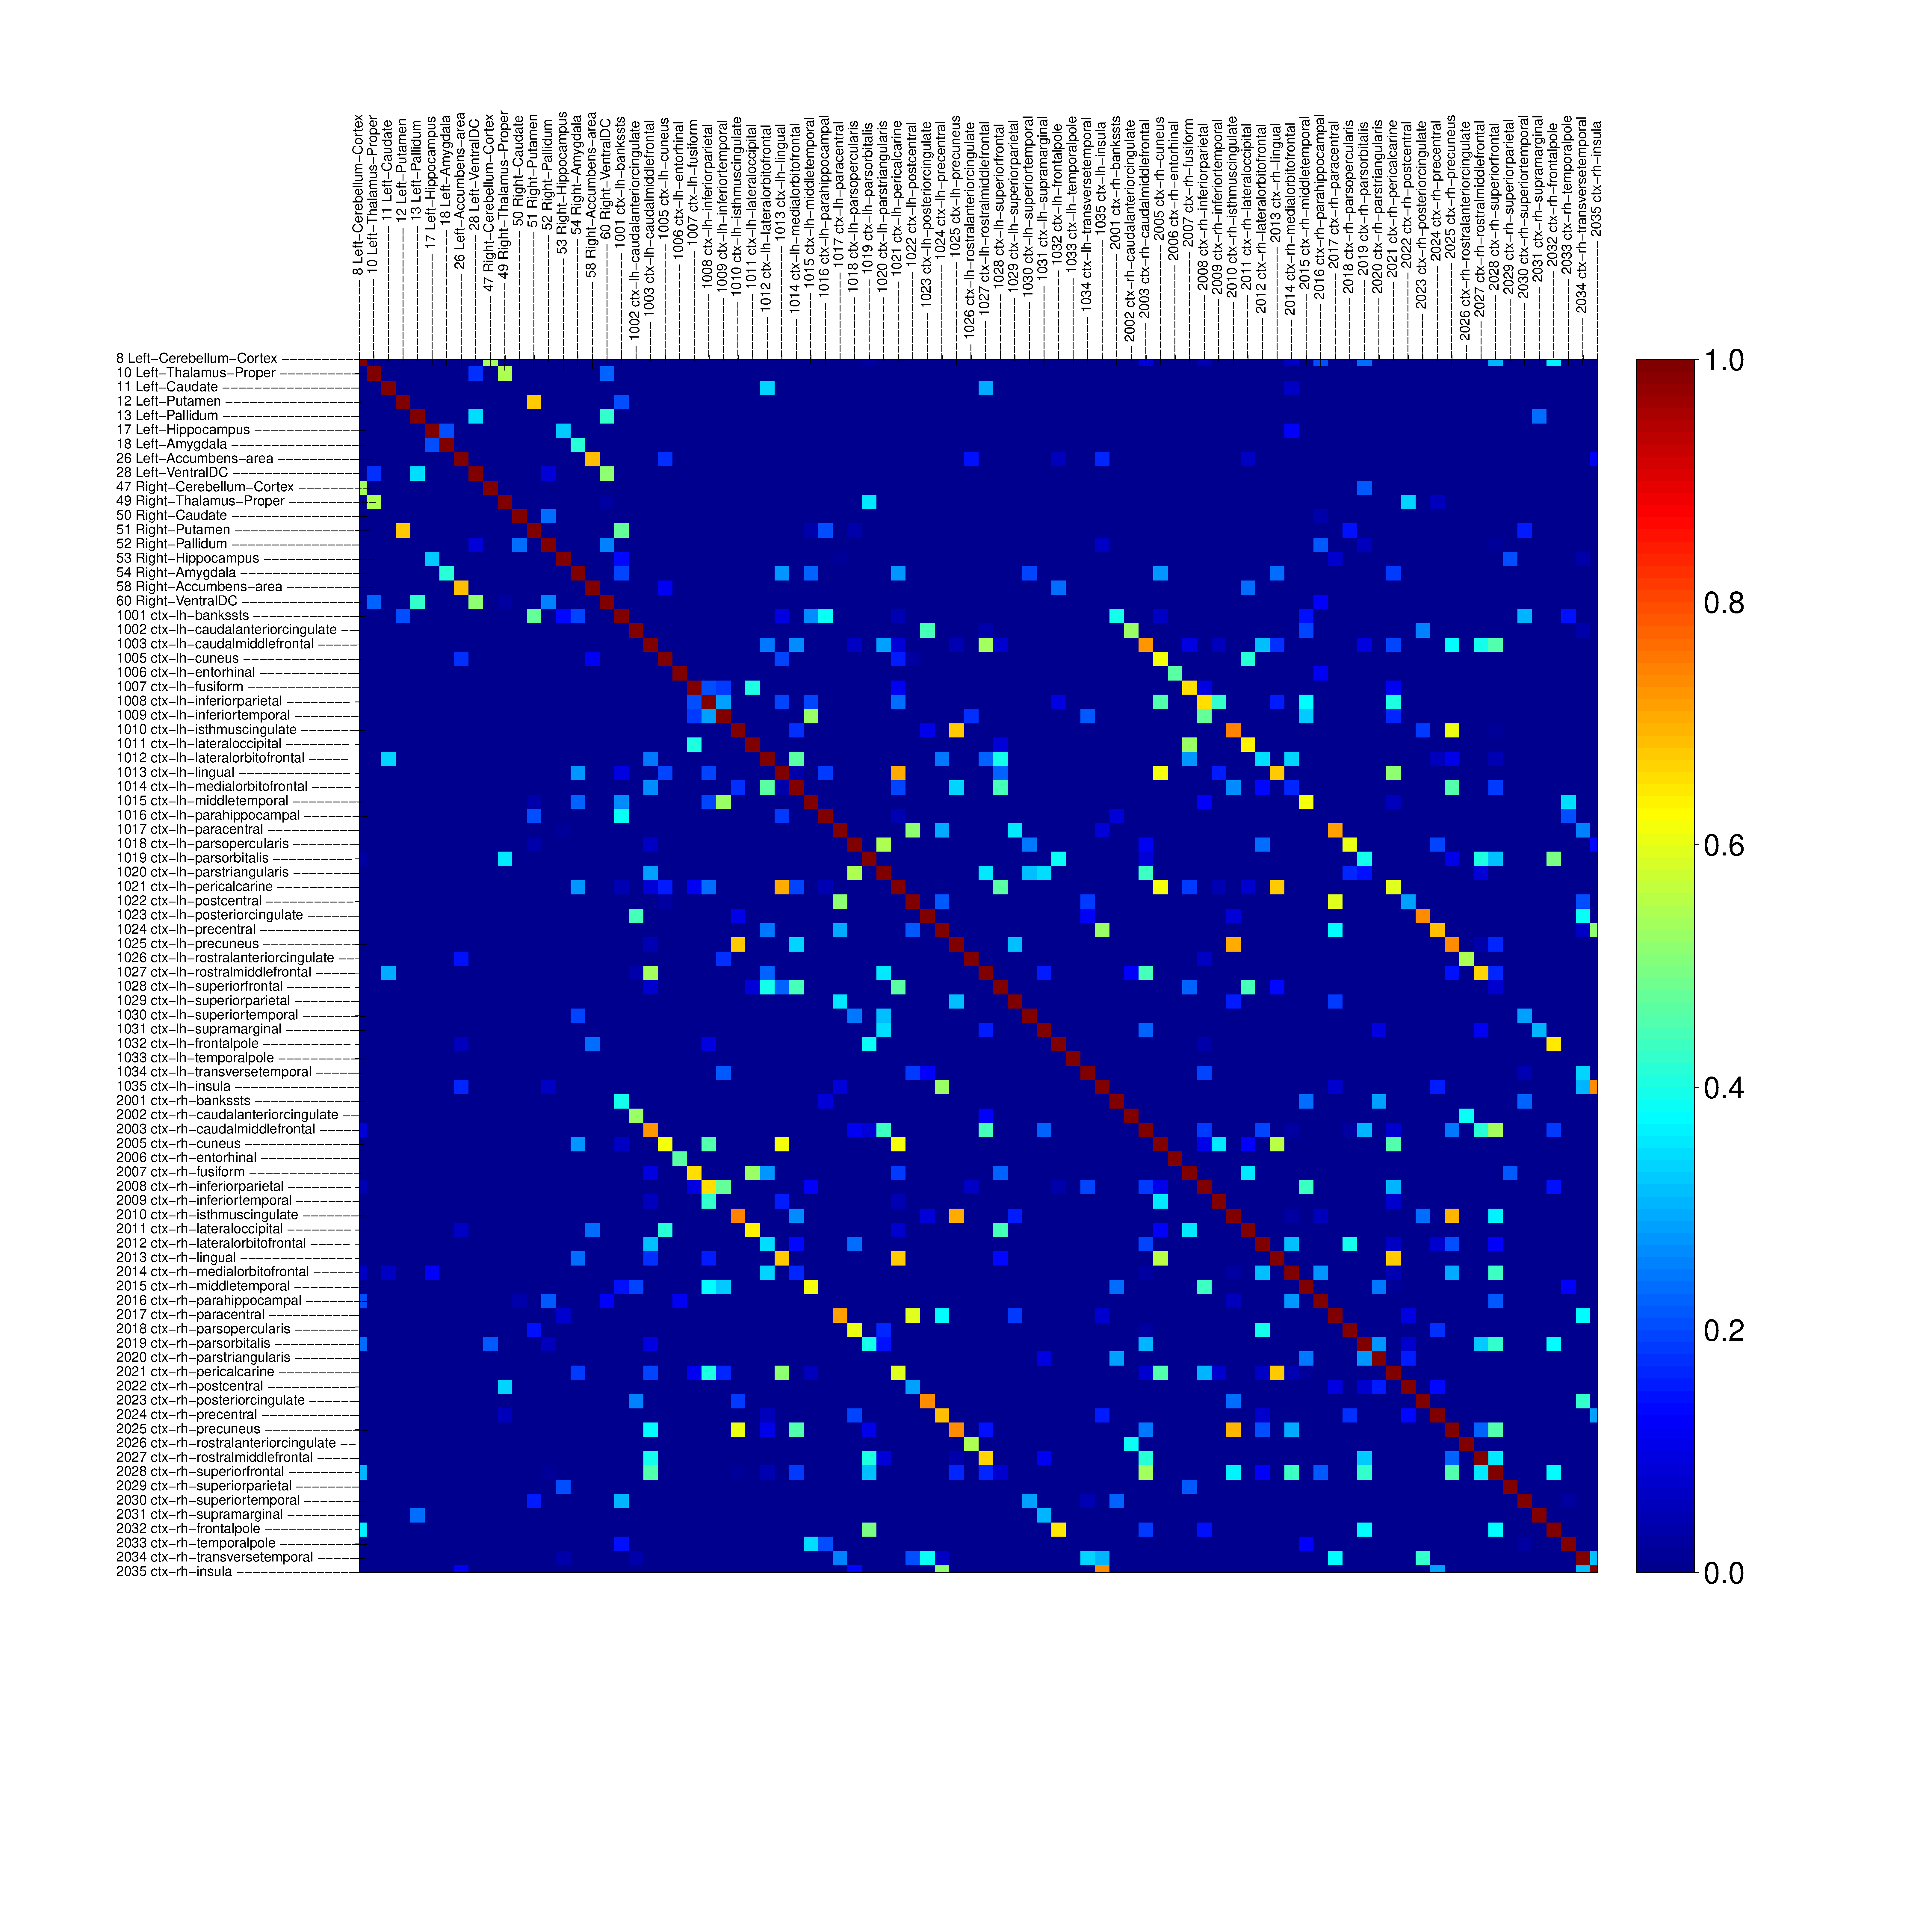
\includegraphics[width=1.1\textwidth]{img/al_hm_0.pdf}
    \caption{Heat map of absolute coherence matrix (at frequency $0$) estimated using adaptive lasso thresholding of averaged periodogram.}
    \label{fig:realdatafullalasso}
\end{figure}

\begin{figure}[p]
    \centering
    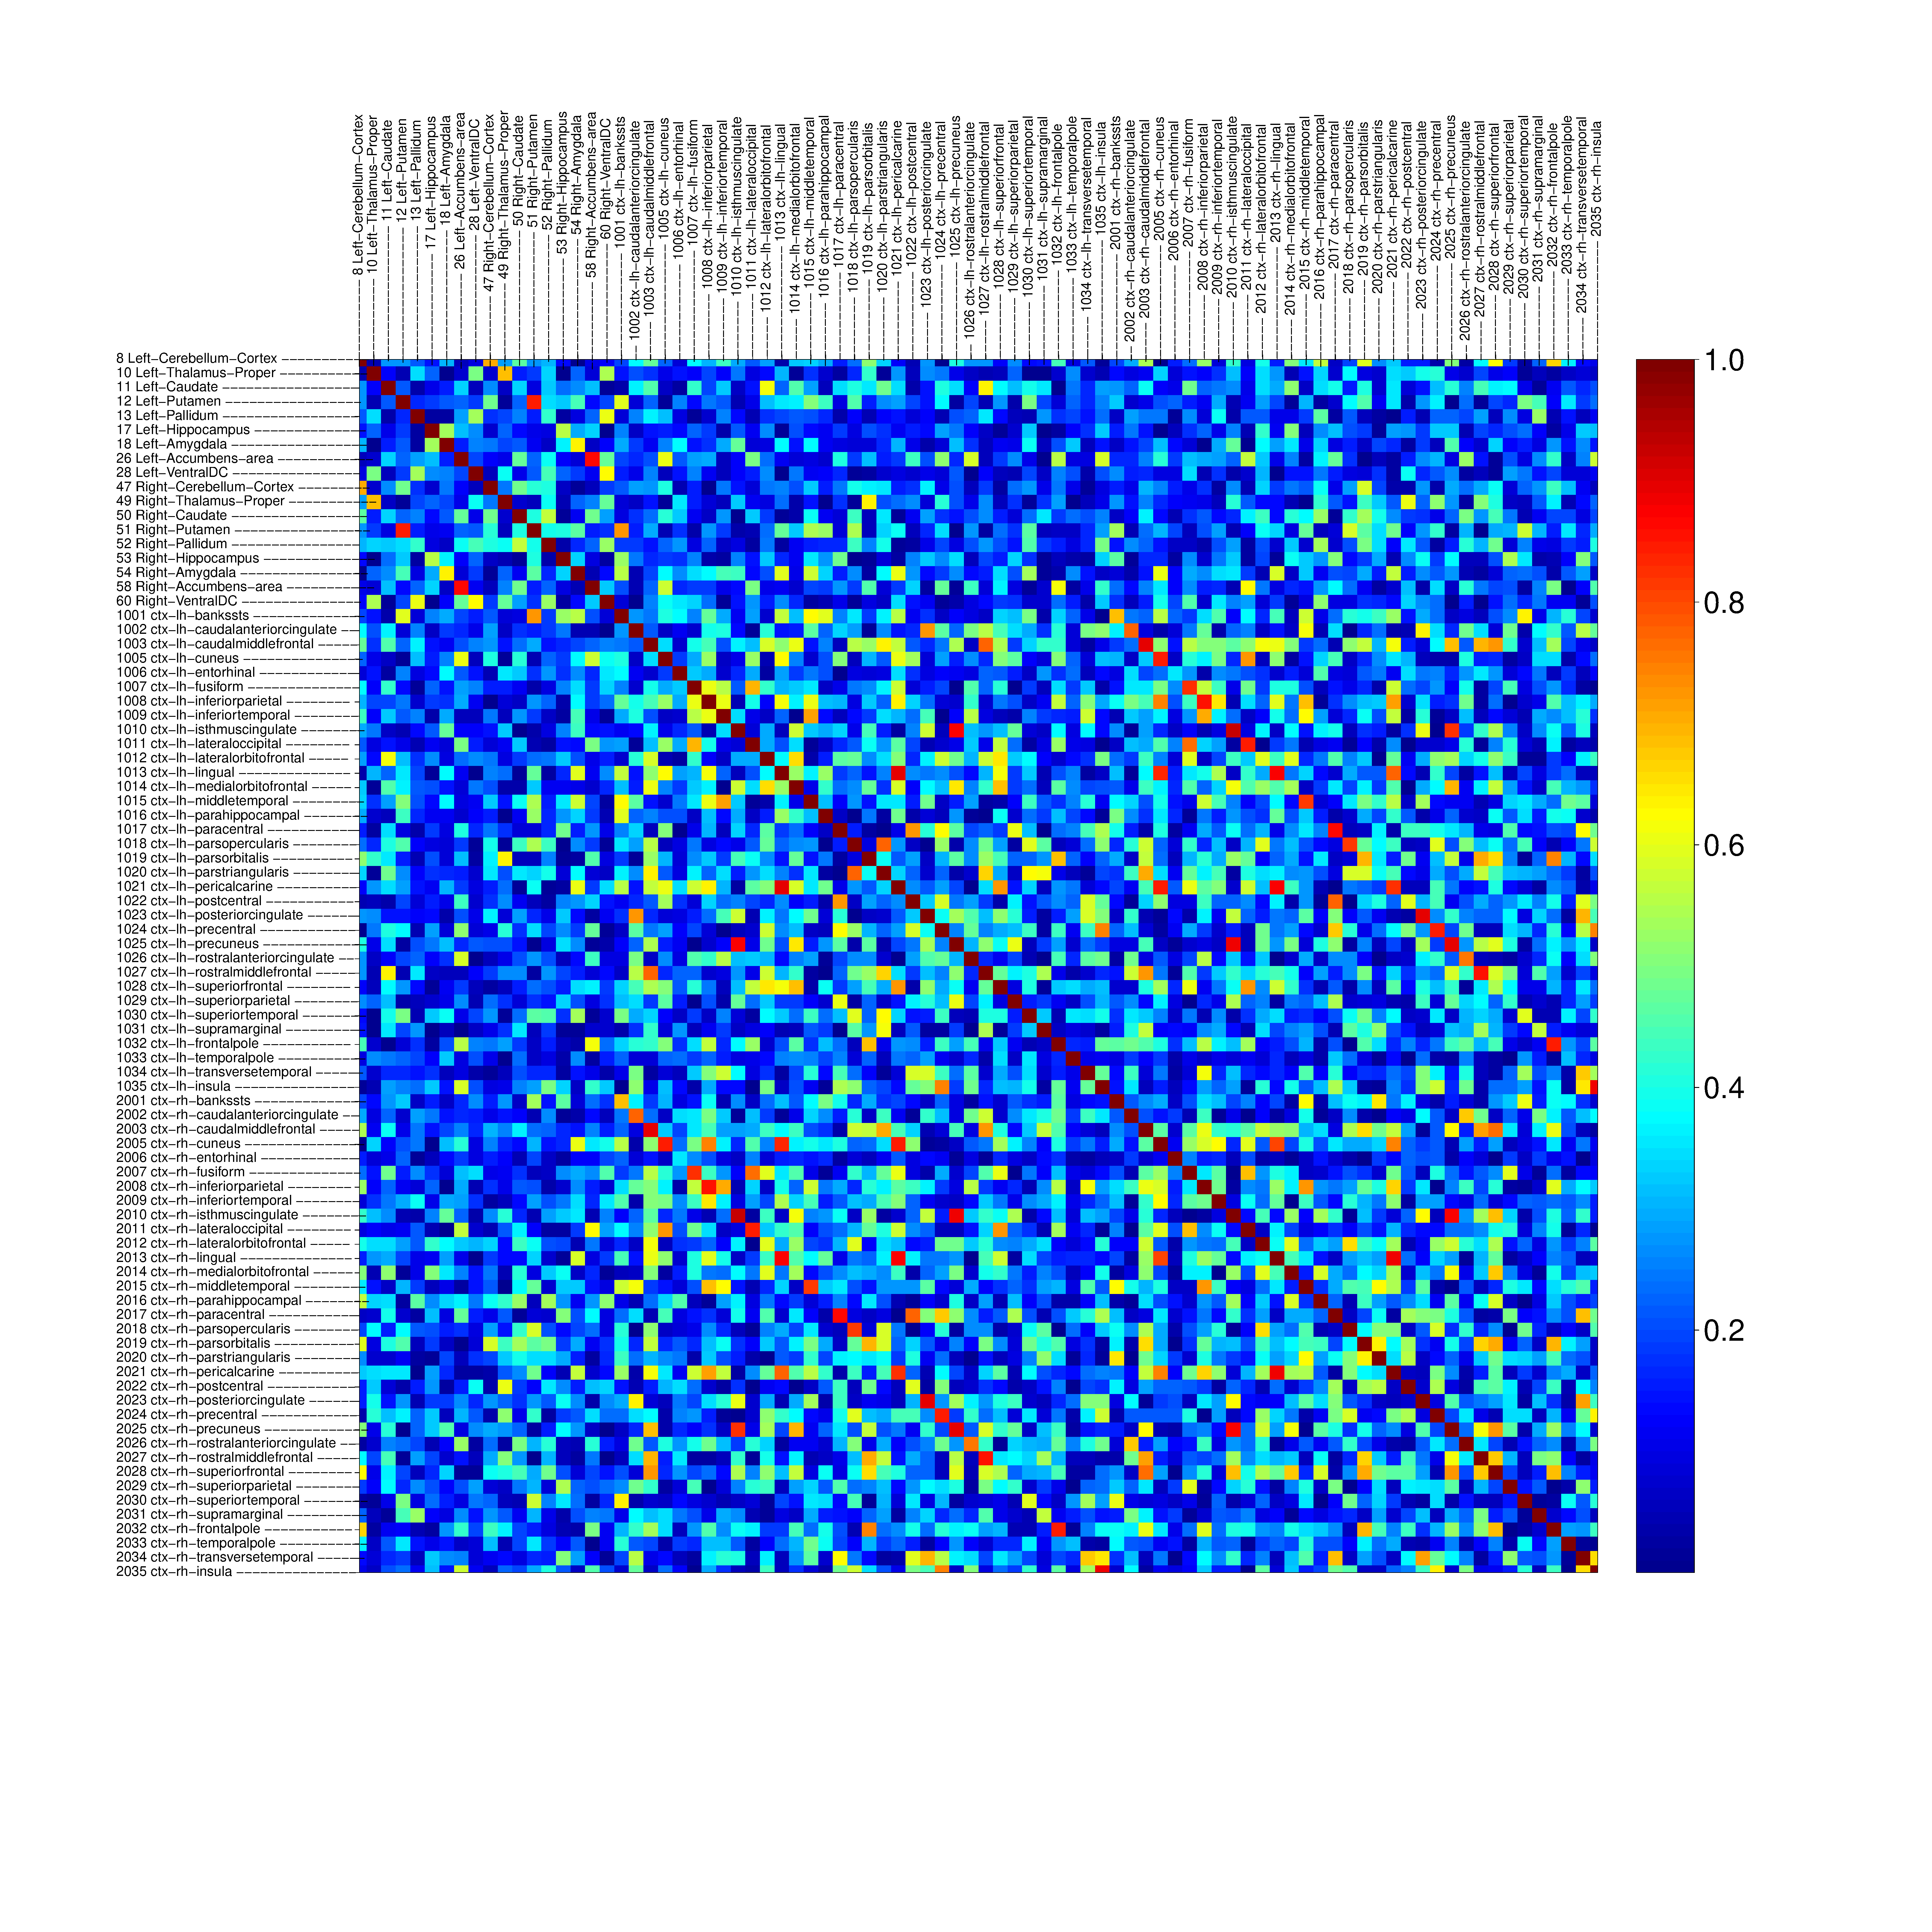
\includegraphics[width=1.1\textwidth]{img/sh_hm_0.pdf}
    \caption{Heat map of absolute coherence matrix (at frequency $0$) estimated using diagonal shrinkage of averaged periodogram.}
    \label{fig:realdatafullshrinkage}
\end{figure}




\end{subappendices}


\chapter{Large Spectral Density Matrix Estimation for Gaussian Process by Adaptive Thresholding}
\section{Introduction}\label{introduction}
Consider a $p$-dimensional real-valued time series $X_t = (X_{t1}, \ldots, X_{tp})^\top, ~ t\in \mathbb{Z}$. It is called weakly stationary if $\E X_t = \E X_s$ and  autocovariance $\Gamma(\ell) = \cov (X_t, X_{t-\ell})$ only depends on the lag $\ell$.  
If for any finite sequence $X_{t_1}, \cdots, X_{t_n})$ and any integer $\tau$, 
$(X_{t_1}, \cdots, X_{t_n})$ has the same joint distribution with  $(X_{t_1+\tau}, \cdots, X_{t_n+\tau})$,  we say the process is strongly stationary. If the joint distribution is multivariate Gaussian, we call this process as Gaussian process where weak stationarity is equivalent to strong stationarity. \par 

For completeness of this chapter, we restate the definition for spectral density for stationary time series in first chapter here. We assume $\mathbb{E} X_t = 0, ~ t=1,\ldots,n$ for ease of exposition. In practice, multivariate time series are often de-meaned before performing correlation based analysis. Strong/Weak stationarity for Gaussian process implies that $\Gamma(\ell) = \cov(X_t, X_{t-\ell}) = \mathbb{E} X_t X_{t-\ell}^\top$ only depends on $\ell$. Spectral density aggregates information of autocovariance of different lag orders $\ell$  at a specific frequency $\omega \in [-\pi, \pi]$ as 
\begin{equation}
\label{eq:def_spectral_density}
f(\omega) = \frac{1}{2\pi}\sum_{\ell=-\infty}^\infty \Gamma(\ell) e^{-\iu \ell \omega }. 
\end{equation}
Note that the autocovariance functions of different lags can be recovered from the spectral density using the transformation  $\Gamma(\ell) =  \int_{-\pi}^{\pi} f(\omega) e^{i\ell \omega} d\omega$, for any $\ell \in \mathbb{Z}$.\par 
Spectral density matrix in Gaussian process is a generalization to covariance matrix for Guassian distribution. For multi-variate Gaussian variable $x$,  position $(r,s)$ for covariance matrix: $\Sigma_{r, s}$ is zero iff variable $x_r, x_s$ are independent with each other. For p dimensional Gaussian process , this equivalent certificate for marginal independence becomes $f_{rs}(\omega) = 0$ for all frequency $\omega\in [-\pi, \pi)$ iff time series $X_r$ is independent of $X_s$. \par 
Recently, researchers have made progresses in developing methods with theoretical support in high-dimension for spectral density estimation for high dimensional time series data, assuming weak sparsity in spectral density, i.e. the $L_1$ norm of the spectral density matrix is small. For example, \cite{fiecas2018spectral, sun2018large} follow a similar path to build theory: first build concentration inequality for smoothing periodogram, then utilize weak sparsity property to demonstrate consistency in estimation. The difference mainly lays in the way of building concentration inequality part, or in other words, the way of measuring the dependency in the data. \cite{fiecas2018spectral} directly uses the magnitude of autocovariance as the measure while \cite{sun2018large} follows the way of measuring dependency from frequency domain perspective as \cite{Basu2015}. Those thresholding
schemes are adaptive to heterogeneity in frequencies, not to variability of the individual entries. In other words, in terms of fixed frequency, they do universal thresholding for the spectral density matrix. In the next subsection, we explain why we need adaptive thresholding for estimating spectral matrix for each fixed frequency. 

\subsection{Why Adaptive Thresholding?}
As pointed by \cite{cai2011adaptive}, universal thresholding was firstly proposed by \cite{donoho1994ideal} for estimating sparse normal mean vectors in the context of wavelet function estimation where noise  is homoscedastic. Although in many cases, the universal thresholding can achieve good theoretical property for heteroscedastic problem within certain weakly sparse space by setting the thresholding value proportional to an upper bound of the standard deviation of the noise.  For example, consider following sparse multivariate Gaussian mean estimation. Suppose that we have n observation of p-variate Gaussian distribution as follows. 
\[
y_i \overset{i.i.d}{\sim} \mathcal{N}\left(\mu, 
\begin{bmatrix}
\sigma^2_1 & 0 & \cdots & 0\\  
0 & \sigma^2_2 & \cdots & 0\\
\vdots & \vdots & \ddots\\
0 & 0& 0& \sigma^2_p
\end{bmatrix}\right),
\]
Each position in the Gaussian vector has different unknown variance $\sigma_j^2$. But if we assume $ \sigma_j$ are uniformly bounded i.e., $\max_j \sigma_j\le B$ for some positive number $B$, 
let $\bar{y}_j = \frac{1}{n}\sum_{i=1}^n y_{ij}$,  and we have 
\begin{equation}
\Prob( |\bar{y}_j  - \mu_j |\ge \eta)\le 2 \exp(-n\eta^2/2\sigma_j^2). 
\end{equation} 
Combine these with techniques introduced in \cite{bickel2008covariance}, if we choose 
threshold to be at order as $B\sqrt{\frac{\log p}{n}}$, we can have asymptotic consistency in estimation of $\mu$ if 
\[
\mu \in \left\{\mu \in \mathbb{R}^p, \sum_{j=1}^p |\mu_j|^q \le c(p)\right\}, 
\]
for some $0\le q<1$ and $c(p)$ is the measure for weak sparsity. The key assumption is that $\sigma_js$ are uniformly bounded. But it is apparent, if $\sigma_j$ variates too much or is not bounded, the argument in \cite{bickel2008covariance} will not work and the accuracy in estimation will get hurt.  So people resort to adaptive thresholding: set the thresholding value to be proportional to an estimator of $\sigma_j$ , say sample standard deviation $\sqrt{\sum_{i=1}^n (y_{ij} - \bar{y}_j)^2/(n-1)}$.  \par 
 Now we go to a more relevant case. 
Consider a number of i.i.d normal distributed $y_i$ with 
\[
y_i \overset{i.i.d}{\sim} \mathcal{N}(0, \Sigma_{p\times p}),
\]
if we want to estimate each position $r, s$ of $\Sigma$: $\Sigma_{rs}$, the estimation problem can be treated as estimating the expectation of $(y_{i}y^\top_{i})_{rs}$. Then maximum likelihood estimator (MLE) is simply the sample average. Suppose the covariance matrix has a weakly sparse structure i.e., a relatively small $L_1$ norm, \cite{bickel2008covariance} proposes to apply universal thresholding 
and they assume diagonal elements for $\Sigma$ are uniformly bounded.  Compared to above sparse mean estimation for multi-variate Gaussian, now it is like the case where we estimate the expectation of a $p^2$ 
random vector $(y_jy_j^\top)_{rs}$, and $\sigma_{rs}^2 = \Var[(y_{i}y^\top_{i})_{rs}] = \Sigma_{rr}\Sigma_{ss} + \Sigma^2_{rs} \le 2\Sigma_{rr}\Sigma_{ss}$. Now it becomes clear why \cite{bickel2008covariance} requires an upper bound for $\Sigma_{rr}$: $2\max_{r=1}^p \Sigma^2_{rr}$ is an upper bound for variance of the target. To conquer the shortcomings we mentioned above about universal thresholding, \cite{cai2011adaptive} proposed adaptive thresholding estimator by setting thresholding value proportional to sample standard deviation of sequence $[(y_1y_1^\top)_{rs}, \cdots, (y_ny_n^\top)_{rs}]$ for $n$ observations. \par 
Now let us go to our case.  As we will introduce later, the spectral density $f(\omega_j)$ can be taken as expectation of $d_\infty (\omega_j) d^\top_\infty (\omega_j)$ where $d_\infty (\omega_j)$ has the distribution same as limiting distribution of discrete Fourier coefficient. Then it is almost same as covariance setting although it is complex matrix not real anymore. \cite{sun2018large} proposes hard thresholding in the modulus of the estimator. With Cauchy-Schwarz inequality, 
\[
\E |( (d(\omega_j)_\infty d(\omega_j)_\infty^\top)_{rs}|^2 \le \E d_{\infty, ss}^2(\omega_j) d_{\infty, rr}^2(\omega_j)\le \esssup_{\omega} \|f(\omega)\|. 
\]
Although \cite{sun2018large} allows $\esssup_{\omega} \|f(\omega)\|$ grow with $n,p$, this upper bound appears in the thresholding value, and its growth rate is required to be controlled.  As discussed before, it is better to replace this upper bound with the estimated variance.  We list our contributions to solve those problems mentioned. 

\begin{itemize}
\item we clearly define the adaptive thresholding estimation problem, and show what variance should our estimator be adaptive to.
\item we propose a modified version of periodogram which assists us to develop the theory for consistent estimation of adaptive thresholding estimator under high dimensional setting.
\item non-asymptotic bound analysis is provided for our adaptive thresholding estimator which relaxes the constraint in operator norm of spectral density for universal thresholding proposed by \cite{sun2018large} and achieves better error bound.
\end{itemize}




\subsection{Periodogram Smoothing}
Let  $\mathcal{X} = [X_1:\ldots:X_n]^\top$  be the \textit{data matrix} containing $n$ consecutive observations from the time series $\{X_t\}$ in its rows. The classical estimate of spectral density is based on the periodogram \citep{brockwell2013time, rosenblatt1985stationary} defined as
\begin{equation}
\label{eq:single_periodogram}
I(\omega)=\sum_{|\ell|<n} \hat{\Gamma}(\ell)e^{-\iu\ell\omega},
\end{equation}
where $\hat{\Gamma}(\ell) = n^{-1}\sum_{t=\ell+1}^{n} X_t X_{t-\ell}^\top$ for $\ell\ge 0$, and 
 $\hat{\Gamma}(\ell) = n^{-1}\sum_{t=1}^{n+\ell} X_t X_{t-\ell}^\top$ for $\ell<0$. It is noticed that the periodogram can be written as outer product of 
Discrete Fourier Transformation(DFT): 
\[
I(\omega) = d(\omega) d^\dag(\omega), 
\]
where $d(\omega)$ is defined as $d(\omega) = \mathcal{X}^\top(C(\omega)-iS(\omega))$ , where 
\begin{equation}
\label{eq:cos_sin_coef}
\begin{aligned}
C(\omega) = \frac{1}{\sqrt{n}} (1, \cos \omega, \dots, \cos (n-1)\omega)^\top,\\
S(\omega) = \frac{1}{\sqrt{n}} (1, \sin \omega, \dots, \sin (n-1)\omega)^\top.
\end{aligned}
\end{equation}
This leads to fast computation with fast Fourier transformation. For brevity,  we let $c_j = C(\omega_j)$ and $s_j = S(\omega_j)$. 
 
It is common to resort to smoothing periodograms over nearby frequencies to achieve asymptotic consistency. The simplest smoothing is 

\begin{equation}
\label{eq:general_smoothing_estimator}
    \hat{f}(\omega; m) = \frac{1}{2\pi(2m+1)} \sum_{|k|\le m} I(\omega+\omega_k),
\end{equation}
where $\omega_k = 2\pi k/n, ~ k\in F_n$,  the set of Fourier frequencies. To be precise, $F_n$ denotes the set  $\left\{-[\frac{n-1}{2}], \dots, [\frac{n}{2}]\right\}$ where $[x]$ is the integer part of $x$. $F_n$ contains exactly the same frequencies used to calculate discrete Fourier transformation. It is common to evaluate the periodogram at these Fourier frequencies, in which case the smoothing periodogram in \eqref{eq:general_smoothing_estimator} becomes
\begin{equation}
\label{eq:smoothing estimator}
    \hat{f}(\omega_j; m) = \frac{1}{2\pi(2m+1)} \sum_{|k|\le m} I(\omega_{j+k}).
\end{equation}
Note that even though the values of $j+k$ can fall outside $F_n$, it is enough to evaluate periodograms at Fourier frequencies $F_n$ since $I(\omega)$ is $2\pi$-periodic in $\omega$. The effectiveness of reducing variance via smoothing lies in the fact that $d(\omega_j), d(\omega_k)$ are asymptotically independent if $k\notin \{-j, j\}$. Since our theory development is based on the asymptotically independence, we change the smoothing set a little bit to make sure that $\{-j, j\}$ would not appear at the same time in the index set. Also, we exclude frequency $0, \frac{\pi}{2}, -\pi$ to avoid degenerate limiting distribution. Then we can present the smoothing periodogram estimator as 
\begin{equation}
g(\omega_j; m) = \frac{1}{m}\sum_{ k\in \mathcal{B}_j^m} I(\omega_k). 
\end{equation}
where $\mathcal{B}_j^m$ is a set containing all indices nearest to $j$ excluding $0, [n/2]$ and all possible pairs $\{j, -j\}$. Assuming $m<n/2$,
in fact the expression for $\mathcal{B}_j^m$ is quite simple
\begin{equation}
\label{eq:def_neb}
\mathcal{B}_j^m = 
\begin{cases}
\{j, j+1, \cdots, j+m\}& j>0 \\
\{j, j-1, \cdots, j-m\}& j<0.
\end{cases}
\end{equation}
as pointed before, we use $2\pi$-periodic in $\omega$ if index falls out of $F_n$. For simplicity, we ignore the m in subscription in $\mathcal{B}_j^m$ and we always let it be $\mathcal{B}_j$. We introduce set $\mathcal{B}_j$ mainly for the purpose of ensuring all $H(\omega_j)$ are asymptotically independents with similar distribution. We exclude pairs like $\{j, -j \}$ and for simplicity, we do not consider frequency $\omega_0, \omega_{[n/2]}$ since they have degenerate limiting distribution. The theory can be easily extended to both cases though. In the next section, we will answer the question: what kind of variance should our thresholding estimator adapt to. \par 


\subsection{What Variance should thresholding Value be Adaptive to?}
In order to derive adaptive thresholding for spectral density estimation, the first question is 
which variance should the estimator be adaptive to? 
Different from i.i.d. Gaussian case, to describe the variance of spectral density, we need to consider the asymptotic distribution of discrete Fourier transformation. We listed Theorem 4.4.1 in  \cite{brillinger2001time} as the following lemma 
\begin{assumption}\label{assumption:finite_auto}
$\sum_{\ell=-\infty}^\infty \|\Gamma(\ell)\|<\infty$. 
\end{assumption}

\begin{lem}
\label{lemma:asy_dis_dft}
Suppose $\mathcal{\mathcal{X}}_{n\times p} = [X_1:\ldots:X_n]^\top$ is a data matrix from a strongly stationary  Gaussian time series $X_t$, and assumption \ref{assumption:finite_auto} is satisfied, we have for all $j\in F_n$ with $\omega_j \neq 0$ or $\pi$, 
\begin{equation}
\label{eq:limiting_dist}
d(\omega_j) = 
\begin{bmatrix}
\mathbf{Re}(d(\omega_j))\\
\mathbf{Im}(d(\omega_j))
\end{bmatrix}=
\begin{bmatrix} 
\mathcal{X}^\top c_j\\
\mathcal{X}^\top s_j
\end{bmatrix}  \overset{d}{\rightarrow} \mathcal{N}\left(0, \frac{1}{2}\begin{bmatrix}
\mathbf{Re}(f(\omega_j) & -\mathbf{Im}(f(\omega_j))\\
\mathbf{Im}(f(\omega_j)) & \mathbf{Re}(f(\omega_j))
\end{bmatrix}
\right).
\end{equation}
For $\omega_j = 0$ or $\omega_j = \pi$, 
\begin{equation}
\mathcal{X}^\top c_j
\overset{d}{\rightarrow} \mathcal{N}\left(0, f(\omega_j)
\right).
\end{equation}
For $k \notin \{j, -j\}$,  
$\begin{bmatrix}
\mathcal{X}^\top c_j\\
\mathcal{X}^\top s_j
\end{bmatrix}$ is asymptotically independent of 
$\begin{bmatrix}
\mathcal{X}^\top c_k\\
\mathcal{X}^\top s_k
\end{bmatrix} $. Here the convergence is convergence in distribution. 
\end{lem} 
This lemma indicates that if we restrict our focus to $\mathcal{B}_j$, all $I(\omega_k), k\in \mathcal{B}_j^m$ are asymptotically independently distributed and within a neighborhood, their asymptotic distributions are very similar to each other, in other words, behave like i.i.d. data. This explains why smoothing periodogram can effectively reduce the variance. What is more, we can treat the spectral density as the expectation of limiting distribution. Let 
$d_{\infty}(\omega_j)$ be the variable whose distribution is the limiting distribution of $d(\omega_j)$, then 
\[
f(\omega_j) = \E(d_{\infty}(\omega_j)d^\dag_{\infty}(\omega_j)).
\]

Now it is clear that the thresholding estimator should adapt to: 
\[
\Var(\mathbf{Re}(d_{\infty}(\omega_j)d^\dag_{\infty}(\omega_j))_{rs}); 
\Var(\mathbf{Im}(d_{\infty}(\omega_j)d^\dag_{\infty}(\omega_j))_{rs})
\]
for position $(r,s)$'s real and imaginary part respectively. Asymptotically, the formation of the problem is almost the same as what is proposed by \cite{cai2011adaptive}: we use sample average of data to estimate its expectation and try to let our estimator be adaptive to its variances. Rearranging those expressions for Gaussian forth moments in appendix, we can express the variances for real and imaginary part of $(d_{\infty}(\omega_j)d_{\infty}(\omega_j)^\dag)_{rs}$ as 
\begin{equation}
\label{eq:variance_of_real_periodogram}
\begin{array}{cc}
&\Var(\mathbf{Re}(d_{\infty}(\omega_j)d^\dag_{\infty}(\omega_j))_{rs})      \\
& = \frac{1}{2}\left[f_{rr}(\omega_j)f_{ss}(\omega_j)+\mathbf{Re}(f_{rs}(\omega_j))^2-\mathbf{Im}(f_{rs}(\omega_j))^2\right]
\end{array}
\end{equation}
and 
\begin{equation}
\label{eq:variance_of_imaginary_periodogram}
\begin{array}{cc}
&\Var(\mathbf{Im}(d_{\infty}(\omega_j)d^\dag_{\infty}(\omega_j))_{rs})      \\
& = \frac{1}{2}\left[f_{rr}(\omega_j)f_{ss}(\omega_j)+\mathbf{Im}(f(\omega_j)_{rs})^2-\mathbf{Re}(f_{rs}(\omega_j))^2\right].
\end{array}
\end{equation}
As mentioned above, the key ingredient in the theoretical development of \cite{cai2011adaptive} is that variances of position $r, s$ of $y_1y_1^\top$ for p variate Gaussian variable $y_1$,  is in the same order of $\Sigma_{rr}\Sigma_{ss}$. However, variances in \eqref{eq:variance_of_real_periodogram} and \eqref{eq:variance_of_imaginary_periodogram}  do not meet this condition. We provide a counter example in Appendix \ref{sec:counter_example} to demonstrate this phenomenon.
We not only utilize the framework provided by \cite{cai2011adaptive}, but also try to avoid diminishing variances in the estimator, which may cause instability in the theory. \par 

\textbf{Notation.} Throughout this paper, $\mathbb{Z}$, $\mathbb{R}$ and $\mathbb{C}$  denote the sets of integers, real numbers and complex numbers, respectively. We use 
$\mathbf{Re}(c)$, $\mathbf{Im}(c)$ to present the real and imaginary part of complex number $c$ respectively and $|c|$ to denote its modulus(absolute value for real number). We use $\|v\|$ to denote $\ell_2$-norm of a vector $v$. For a matrix $A$, $\|A\|_1$, $\|A\|_{\infty}$, $\|A\|$ and $\|A\|_F$ will denote maximum complex modulus column sum norm, maximum complex modulus row sum norm, { spectral norm} $\sqrt{\Lambda_{\max}(A^\dag A)}$ and Frobenius norm $\sqrt{\text{tr}(A^\dag A)}$, respectively, where $A^\dag$ is the conjugate transpose of $A$.  We use $e_i$ to denote the $i^{th}$ unit vector in $\mathbb{R}^p$, for $i = 1, 2, \ldots, p$. Also, we let $E_p$ be the set containing $e_1, \cdots, e_p$. 
For vectors $v_i \in \mathbb{R}^p, i=1,\ldots, n$, we use $[v_1:\ldots:v_n]$ to denote the $p \times n$ matrix formed  by horizontally stacking these column vectors $v_i$, and  $[v_1^\top;\ldots; v_n^\top]$ to denote the $n\times p$ matrix by vertically stacking row vectors $v_i^\top$. Let $vec(A)$ represent the vector obtained from vectorization of a matrix $A$ by stacking all its columns. We use $rk(A)$ to denote the rank of a matrix $A$. For a complex vector $v\in \mathbb{C}^p$ and any $q > 0$, we define $\|v\|_q:= (\sum_{i=1}^p |v_i|^q)^{1/q}$. We use $\|v\|_0$ to denote the number of non-zero elements in $v$. Note that when $0\le q<1$, it is not really a norm, for triangle inequality does not hold, but we keep the notation of a norm for convenience. Then we define the induced matrix norm, $\|A\|_{\alpha, \beta} = \sup_{x\neq 0}\|Ax\|_\alpha/\|x\|_\beta$, for any  $\alpha>0, \beta>0$. We will also use $\|A\|_\alpha$ to denote the induced norm $\|A\|_{\alpha, \alpha}$ for any $\alpha > 0$ and any complex matrix $A \in \mathbb{C}^{p \times p}$. Also, to be succinct, we use $\|A\|_{\rm{max}} :=\max_{r,s}|A_{rs}|$. 
Throughout the paper, we write $A \succsim B$ if there exists a  universal constant $c > 0$, not depending on model dimension or any model parameters, such that $A \ge cB$. We use $A \asymp B$ to denote $A \succsim B$ and $B \succsim A$.  










\section{Background and Methods}
\label{sec:model-methods}
\subsection{Modified Periodogram and Its Smoothing Estimator}
In this section, we show that with only a small but effective modification in periodogram, we can still preserve asymptotic unbiasedness while letting the order of the variance for each entry $(r,s)$ still at $f_{rr}(\omega_j)f_{ss}(\omega_j)$. \par  
\begin{equation}
\begin{aligned}
f(\omega_j) & = \E [d_\infty (\omega_j) d^\top_\infty (\omega_j)]  \\
&  = \E [ {\bf Re}(d_\infty (\omega_j)){\bf Re}(d^\top_\infty (\omega_j)) + 
{\bf Im}(d_\infty (\omega_j)){\bf Im}(d^\top_\infty (\omega_j)) ] \\
& + i\E [ {\bf Im}(d_\infty (\omega_j)){\bf Re}(d^\top_\infty (\omega_j)) -
{\bf Re}(d_\infty (\omega_j)){\bf Im}(d^\top_\infty (\omega_j)) ]
\end{aligned}
\end{equation}
Lemma \ref{lemma:asy_dis_dft} claims that 
${\bf Re}(d_\infty (\omega_j))$ and ${\bf Im}(d_\infty (\omega_j))$ share the same marginal distribution,  and  
$\E [ {\bf Im}(d_\infty (\omega_j)){\bf Re}(d^\top_\infty (\omega_j)) = -\E 
{\bf Re}(d_\infty (\omega_j)){\bf Im}(d^\top_\infty (\omega_j)) $.  Then we have for real and imaginary parts of spectral density, 
\begin{equation}
\begin{array}{cc}
& \mathbf{Re}(f(\omega_j)) = 2 \E \mathbf{Re}(d_{\infty}(\omega_j))  \mathbf{Re}(d_{\infty}(\omega_j))^\top  \\
& \mathbf{Im}(f(\omega_j)) = 2\E \mathbf{Im}(d_{\infty}(\omega_j))  \mathbf{Re}(d_{\infty}(\omega_j))^\top 
\end{array}
\end{equation}
where $d_{\infty}(\omega_j)$'s distribution is the same as the limiting distribution of $d(\omega_j)$. Therefore, we could use
\begin{equation}
H(\omega_j) = 2\mathbf{Re}(d(\omega_j))  \mathbf{Re}(d(\omega_j))^\top+2\mathbf{Im}(d(\omega_j))  \mathbf{Re}(d(\omega_j))^\top i
\end{equation}
as our modified periodogram, with its limiting version of
\begin{equation}
H_\infty(\omega_j) = 2\mathbf{Re}(d_{\infty}(\omega_j))  \mathbf{Re}(d_{\infty}(\omega_j))^\top+2\mathbf{Im}(d_{\infty}(\omega_j))  \mathbf{Re}(d_{\infty}(\omega_j))^\top i
\end{equation}
whose expectation is exactly $f(\omega_j)$. Then the variance for 
real and imaginary parts of $H_{\infty, rs}(\omega_j)$ can be calculated with fourth moments of Gaussian distribution: 
\begin{equation}
\begin{array}{cc}
\Var(\mathbf{Re}(H_{\infty, rs}(\omega_j))) = \left[f_{rr}(\omega_j)f_{ss}(\omega_j)+\mathbf{Re}(f_{rs}(\omega_j))^2\right]
\end{array}
\end{equation}
and 
\begin{equation}
\begin{array}{cc}
\Var(\mathbf{Im}(H_{\infty, rs}(\omega_j))) = \left[f_{rr}(\omega_j)f_{ss}(\omega_j)+\mathbf{Im}(f_{rs}(\omega_j))^2\right].
\end{array}
\end{equation}
Both of them are at the same order of $f_{rr}(\omega_j)f_{ss}(\omega_j)$. More specifically,
\begin{equation}
\begin{aligned}
& f_{rr}(\omega_j)f_{ss}(\omega_j)\le \Var({\bf Re}(H_{\infty, rs}))\le 2f_{rr}(\omega_j)f_{ss}(\omega_j) \\
& f_{rr}(\omega_j)f_{ss}(\omega_j)\le \Var({\bf Im}(H_{\infty, rs}))\le 2f_{rr}(\omega_j)f_{ss}(\omega_j)
\end{aligned}
\end{equation}
In the following, we will show how to use the modified periodogram to perform adaptive thresholding. The modified smoothing periodogram can be written as 
\begin{equation}
g(\omega_j) = \frac{1}{m}\sum_{k\in \mathcal{B}_j} H(\omega_k). 
\end{equation}



\subsection{Method: Adaptive Thresholding}
Firstly we introduce definition of generalized thresholding proposed by \cite{rothman2009generalized}: consider a thresholding operator $S_\lambda(\cdot)$ that integrates the benefits of shrinkage and thresholding: 
\begin{enumerate}[(1)]
\item $|S_\lambda(z)|\le |z|$,
\item $S_\lambda(z) = 0$ if $|z|\le \lambda$,
\item $|S_\lambda(z)-z|\le \lambda $.
\end{enumerate}
\cite{rothman2009generalized} show that this estimator can recover the covariance matrix assuming weak sparsity. \cite{cai2011adaptive} further let the thresholding value be proportional to the estimator of standard deviation. 


\paragraph{Estimation of Variance:}
As pointed out above, all $H(\omega_k), k\in \mathcal{B}_j$ behave like i.i.d. variables, thus we propose to use sample variance to estimate variances at position $(r, s)$ of ${\bf Re}(H(\omega_j))$ and 
${\bf Im}(H(\omega_j))$. We let $\theta^{(r)}_{j, rs}$ represent  $\Var({\bf Re}(H_{\infty, rs}(\omega_j)))$ and $\theta^{(i)}_{j, rs}$ represent $\Var({\bf Im}(H_{\infty, rs}(\omega_j)))$ respectively.  Then we can write the estimator $\hat{\theta}^{(r)}_{j,rs}$,  $\hat{\theta}^{(i)}_{j,rs} $ as 
\begin{equation}
\label{eq:variance_estimator}
\begin{aligned}
& \hat{\theta}^{(r)}_{j,rs} = \frac{1}{m-1}\sum_{q\in \mathcal{B}_j} \left[{\bf Re}(H_{rs}(\omega_q)) - \frac{1}{m}\sum_{k\in \mathcal{B}_j} {\bf Re}(H_{rs}(\omega_k))\right]^2 \\
&\hat{\theta}^{(i)}_{j,rs} = \frac{1}{m-1}\sum_{q\in \mathcal{B}_j} \left[{\bf Im}(H_{rs}(\omega_q)) - \frac{1}{m}\sum_{k\in \mathcal{B}_j} {\bf Im}(H_{rs}(\omega_k))\right]^2. 
\end{aligned}
\end{equation}

\paragraph{Adaptive Estimator}
With the variance estimator,  the adaptive thresholding value for the real and imaginary parts at frequency $\omega_j$ at position $(r, s)$, which we call $\lambda^{(r)}_{rs}$ and $\lambda^{(i)}_{rs}$ respectively, will look like
\begin{equation}
\begin{aligned}
& \lambda^{(r)}_{rs} = \sqrt{\hat{\theta}^{(r)}_{j, rs}} \lambda^{(r)} \\
& \lambda^{(i)}_{rs}= \sqrt{\hat{\theta}^{(i)}_{j, rs}} \lambda^{(i)}.
\end{aligned}
\end{equation}
Here $\lambda^{(r)}, \lambda^{(i)}$ are the same across all positions for spectral density at frequency $\omega_j$ for real and imaginary part respectively. We delete $j$ from notation for brevity.  


Let $\hat{\theta}_j^{(r)}$ be the matrix of size $p\times p$, with each element equal to  $\hat{\theta}^{(r)}_{j, rs}$ and we define $\hat{\theta}_j^{(i)}$ in a similar way. For the real part, we can  define following adaptive thresholding operator:
\begin{equation}
T_{\hat{\theta}_j^{(r)}\lambda} (M) = \tilde{M} 
\end{equation}
where 
\begin{equation}
\tilde{M} (r, s) = \begin{cases}
M(r, s) & ~\text{if}~ |M(r, s)| \le \sqrt{\hat{\theta}^{(r)}_{j, rs}}\lambda  \\
0 & \text{else}
\\
\end{cases}
\end{equation}
We present the way to choose $\lambda^{(r)}_j$ for the real part in Algorithm \ref{alg:sample-split-real}, which also applies to choosing the threshold value for the imaginary part. 



\begin{algorithm2e}[t]\small
	\DontPrintSemicolon 
	\KwIn{$j, m, N$, modified periodograms at Fourier frequency $H(\omega_j)$,  an estimator of variance 
		of real part $\hat{\theta}^{(r)}_j$, finite grid of thresholds $\mathcal{L}$}
	\For{$\lambda \in \mathcal{L}$}{
		\For{$\nu \gets 1$ \textbf{to} $N$}{
			Randomly divide $\mathcal{B}_j$ into two subsets $J_1$ and $J_2$ such that $\left||J_1| - |J_2| \right| \le 1$ \;
			$g_{1, \nu} (\omega_j) \gets \frac{1}{|J_1|}\sum_{k \in J_1} {\bf Re}(H(\omega_k))$, ~~ $g_{2, \nu} (\omega_j) \gets \frac{1}{|J_2|}\sum_{k \in J_2} H(\omega_k)$\;
			$\hat{R}_{\nu}(\omega_j, \lambda) \gets \left\| T_{\hat{\theta}^{(r)}_j\lambda} (g_{1,\nu} (\omega_j)) - g_{2,\nu}(\omega_j)\right\|^2_F$\;
		}
		$\hat{R}(\omega_j, \lambda) \gets \sum_{\nu=1}^N \hat{R}_{\nu}(\omega_j, \lambda) / N$
		
	}
	\KwOut{$\hat{\lambda}_j := \hat{\lambda}(\omega_j) = \argmin_{\lambda \in \mathcal{L}} \hat{R}(\omega_j, \lambda)$}
	\caption{Threshold Selection by Frequency Domain Sample-splitting for Real Part}
	\label{alg:sample-split-real}
	\label{al1}
\end{algorithm2e}



\section{Theoretical Properties}\label{sec:theory}
In this section, we analyze asymptotic properties of adaptive thresholding average modified periodograms. First we need to present the bound for bias in the average modified periodogram and variance estimator. Then we build concentration inequality for estimators of both of them. 


\subsection{Bounding the Bias}
Although the modified periodograms $H(\omega_k), k\in \mathcal{B}_j$  are asymptotically independent, and behave like i.i.d., we need to quantify the bias from two sources. One is from the gap between the finite sample to the limiting distribution; the other is from the fact that the limiting distributions are not exactly identical. In this section, we list the results of bounding the bias for both smoothing modified periodograms and variance estimator. \par 

Our process requires some conditions in the minimal value of diagonal of spectral density. 
\begin{assumption}
$\min_{r=1}^p f_{rr}(\omega_j) \ge \phi_0 > 0$.
\end{assumption}
For simplicity we give a deterministic lower bound for diagonal elements in spectral density. 

\paragraph{Bias for Smoothing Modified Periodogram} Similar to \cite{sun2018large}, two quantities are needed that capture the strength of temporal and contemporaneous dependence in the multivariate time series $\{X_t\}_{t \in \mathbb{Z}}$ , which are 
\begin{eqnarray}
\Omega_{n} = \max_{1 \le r,s \le p} \sum_{\ell=-n}^n |\ell| |\Gamma_{rs}(\ell)|, ~~~~ L_n = \max_{1 \le r,s \le p}\sum_{|\ell|>n} |\Gamma_{rs}(\ell)|.
\end{eqnarray}
\begin{lem}
\label{lemma:bound_deviation}
For any $j\in F_n$, $1\le r, s\le p$, 
\begin{equation}
\begin{aligned}
&\max\left\{\left|\mathbb{E}[{\bf Re}(g_{rs}(\omega_j))] - {\bf Re}(f_{rs}(\omega_j))\right|, \left|\mathbb{E}[{\bf Im}(g_{rs}(\omega_j))] - {\bf Im}(f_{rs}(\omega_j))\right|\right\} \le B_f,
\end{aligned}
\end{equation}
where $B_f = \frac{m}{n}\Omega_n + \frac{1}{2\pi}\left(\frac{\Omega_n}{n}+L_n\right) +\frac{\Omega_n}{2\pi n}$.
\end{lem}
The technique for proof starts with the triangular inequality, 
\begin{equation}
\begin{aligned}
&\left|\E[{\bf Re}(g_{rs}(\omega_j))] - {\bf Re}(f_{rs}(\omega_j))\right| \\
&\le \left|\E[{\bf Re}(g_{rs}(\omega_j))] - \E[{\bf Re}(\hat{f}_{rs}(\omega_j))]\right|+\left|\E[{\bf Re}(\hat{f}_{rs}(\omega_j))] - {\bf Re}(f_{rs}(\omega_j))\right|, 
\end{aligned}
\end{equation}
where the bound for the second part is already shown in \cite{sun2018large}, and the first part of above inequality we can handle properties of toeplitz matrices. We defer the detailed proof to Appendix. 
\paragraph{Bias for Variance Estimation}
\begin{lem}
\label{lemma:theta_bias}
\begin{equation}
\begin{aligned}
&\max\left\{\left|\mathbb{E} \hat{\theta}^{(r)}_{j,rs} - \theta^{(r)}_{j, rs}\right|,  \left|\mathbb{E} \hat{\theta}^{(i)}_{j,rs} - \theta^{(i)}_{j, rs}\right|\right\}\le B_\theta,
\end{aligned}
\end{equation}
where $B_\theta = 2\max (f_{rr}(\omega_j),f_{ss}(\omega_j))(\delta_1+\delta_2)+\delta_1^2+\delta_2^2+\frac{\Omega_n^2}{\pi^2n^2}$,
and 
\begin{equation}
\label{eq:def_delta12}
\begin{aligned}
&\delta_1 = \frac{\Omega_n}{2n\pi}+\frac{\sqrt{2}}{2\pi}\frac{m\Omega_n}{n}+ \frac{1}{2\pi}\left(\frac{\Omega_n}{n} + L_n\right) \\
&\delta_2=\frac{\Omega_n}{2n\pi}+ \frac{1}{2\pi}\left(\frac{\Omega_n}{n} + L_n\right).
\end{aligned}
\end{equation}
\end{lem}
\begin{remark}
Assuming $\Omega_n,  f_{rr}$ is bounded, then the bias in variance estimation has the same order of bias for estimator $g_{rs}(\omega_j)$: $\mathcal{O}(m/n)$. 
\end{remark}
The proof is deferred to Appendix. 
Based on the bound for variance estimation, we here present another useful result. Since our intuition is that asymptotically modified periodograms are behaving like i.i.d. within $\mathcal{B}_j$, we expect that   
\begin{equation}
\begin{aligned}
& \Var({\bf Re}(g_{rs}(\omega_j))) \approx \frac{1}{m} \theta^{(r)}_{j, rs}\\ 
& \Var({\bf Im}(g_{rs}(\omega_j))) \approx \frac{1}{m} \theta^{(i)}_{j, rs}.
\end{aligned}
\end{equation}
The following lemma justifies and quantifies the above intuition. 
\begin{lem}
For $1\le r, s\le p$, 
\label{lemma: variance_ratio_error}
\begin{equation}
\begin{aligned}
& \frac{1}{m}(1-B_\delta) \le \min\left\{\left|\frac{\Var({\bf Re}(g_{rs}(\omega_j)))}{\theta^{(r)}_{j, rs}}\right|, \left|\frac{\Var({\bf Im}(g_{rs}(\omega_j)))}{\theta^{(i)}_{j, rs}}\right|\right\}\\
& \le \max\left\{\left|\frac{\Var({\bf Re}(g_{rs}(\omega_j)))}{\theta^{(r)}_{j, rs}}\right|, \left|\frac{\Var({\bf Im}(g_{rs}(\omega_j)))}{\theta^{(i)}_{j, rs}}\right|\right\} \le \frac{1}{m}(1+B_\delta),
\end{aligned}
\end{equation}
where $B_\delta = 4\delta_1/\phi_0 + 3\delta_1^2/\phi_0^2$, $\delta_1, \delta_2$ follow the definition in Lemma \ref{lemma:theta_bias}. 
\end{lem}


\subsection{Deviation Bound} 
In the previous section,  we have shown the upper bound for bias for $g_{rs}(\omega_j)$, $\hat{\theta}^{(r)}_{j, rs}$ and $\hat{\theta}^{(i)}_{j, rs}$. In this section, we will build the non-asymptotic analysis for those estimators. The non-asymptotic analysis will lead to the
main theory for consistency of our adaptive thresholding estimators. 


\begin{lem}
\label{lemma: deviation_variance}
For any positive number $\eta>0$, there exit constants $c_1, c_2$ s.t.
\begin{equation}
\begin{aligned}
& \mathbb{P}\left(\left|\hat{\theta}^{(r)}_{j, rs} - \theta^{(r)}_{j, rs}\right|\ge  
B_\theta + \eta \right) \le  c_1\exp(-c_2m\min\left(\eta, \eta^2\right)), \\ 
& \mathbb{P}\left(\left|\hat{\theta}^{(i)}_{j, rs} - \theta^{(i)}_{j, rs}\right|\ge  
B_\theta + \eta \right) \le  c_1\exp(-c_2m\min\left(\eta, \eta^2\right)).\\ 
\end{aligned}
\end{equation}
\end{lem}
The next lemma constitutes the key element for theoretical development. It is a non-asymptotic analysis. 
\begin{lem}
For $j\in F_n$, and $\omega_j \notin \{0, -\pi\}$,  $1\le r, s\le p$, 
assuming $B_\delta\le 3$ and $B_\theta/\phi_0^2<1/4$, given $\eta\le 1$, there exist universal positive constants $c_1, c_2$, s.t. 
\begin{equation}
\begin{aligned}
& \Prob\left(\left|\frac{{\bf Re}(g_{rs}(\omega_j)) - {\bf Re}(f_{rs}(\omega_j))}{\sqrt{\hat{\theta}^{(r)}_{j,rs}}}\right| \ge \frac{B_f}{\phi_0}+\eta\right)\le c_1\exp(-c_2\min(\eta^2 m, \eta \sqrt{m})),\\
& \Prob\left(\left|\frac{{\bf Im}(g_{rs}(\omega_j)) - {\bf Im}(f_{rs}(\omega_j))}{\sqrt{\hat{\theta}^{(i)}_{j,rs}}}\right| \ge \frac{B_f}{\phi_0}+\eta\right)\le c_1\exp(-c_2\min(\eta^2 m, \eta \sqrt{m})).
\end{aligned}
\end{equation}
\end{lem}
\begin{remark}
The conditions like $B_\delta\le 3$ and $B_\theta/\phi_0^2<1/4$ are set for convenience of proof. In the later main results section, asymptotically, they both go to zero. 
\end{remark}

\begin{proof}
We will focus on the proof for the real part. First we handle the bias. 
Define event $\mathcal{A}_j$ and $\mathcal{B}_j$ as 
\begin{equation}
\begin{aligned}
& \mathcal{A}_j = \{\hat{\theta}^{(r)}_{j, rs}\le (4 - B_\theta/\phi_0^2) \theta^{(r)}_{j,rs} \},\\
& \mathcal{B}_j = \{\hat{\theta}^{(r)}_{j, rs}\ge (1/4 + B_\theta/\phi_0^2) \theta^{(r)}_{j, rs} \}.
\end{aligned}
\end{equation}
Given lemma \ref{lemma: deviation_variance} and the fact that $\theta^{(r)}_{j, rs}$ is at the same order of $f_{rr}(\omega_j)f_{ss}(\omega_j)$:
\begin{equation}
f_{rr}(\omega_j)f_{ss}(\omega_j)\le \theta^{(r)}_{j, rs}\le  2f_{rr}(\omega_j)f_{ss}(\omega_j). 
\end{equation}
We can show that there exist universal constants $c_1, c_2$ only depending on $\phi_0$
\begin{equation}
\begin{aligned}
&\mathbb{P} (\mathcal{A}_j^c) \le \mathbb{P}\left(|\hat{\theta}^{(r)}_{j, rs} - \theta^{(r)}_{j, rs}|\ge (3 +B_\theta/\phi_0^2 )f_{rr}(\omega_j)f_{ss}(\omega_j)\right)\\
& \le c_1\exp\{-c_2m\}.
\end{aligned}
\end{equation}
Similarly we can obtain the same bound for $\mathbb{P}(\mathcal{B}_j^c)$. From now on we restrict our analysis to the event $\mathcal{A}_j$ and $\mathcal{B}_j$. \par 
By triangular inequality,  
\begin{equation}
\begin{aligned}
& \left|\frac{{\bf Re}(g_{rs}(\omega_j)) - {\bf Re}(f_{rs}(\omega_j))}{\sqrt{\hat{\theta}^{(r)}_{j,rs}}}\right| \\
& \le \left|\frac{{\bf Re}(g_{rs}(\omega_j)) - \E {\bf Re}(g_{rs}(\omega_j))}{\sqrt{\hat{\theta}^{(r)}_{j,rs}}}\right|\\
& +  \left|\frac{\E {\bf Re}(g_{rs}(\omega_j)) -{\bf Re}(f_{rs}(\omega_j))}{\sqrt{\hat{\theta}^{(r)}_{j,rs}}}\right|. 
\end{aligned}
\end{equation}
Noticing on event $\mathcal{B}_j$, 
\begin{equation}
 \left|\frac{\E {\bf Re}(g_{rs}(\omega_j)) -{\bf Re}(f_{rs}(\omega_j))}{\sqrt{\hat{\theta}^{(r)}_{j,rs}}}\right|\le 2B_f/\phi_0,
\end{equation}
which indicates that 

\begin{equation}
\begin{aligned}
& \Prob\left(\left|\frac{{\bf Re}(g_{rs}(\omega_j)) - {\bf Re}(f_{rs}(\omega_j))}{\sqrt{\hat{\theta}^{(r)}_{j,rs}}}\right| \ge \frac{B_f}{\phi_0}+\eta\right) \\
& \le \Prob\left(\left|\frac{{\bf Re}(g_{rs}(\omega_j)) - \E {\bf Re}(g_{rs}(\omega_j))}{\sqrt{\hat{\theta}^{(r)}_{j,rs}}}\right| \ge \eta\right) .
\end{aligned}
\end{equation}
On event  $\mathcal{A}_j$, 
\[
\sqrt{\frac{\hat{\theta}^{(r)}_{j, rs}}{\theta^{(r)}_{j, rs}}} \le 2. 
\]

We write the left part of the result for the real part as  
\begin{equation}
\begin{aligned}
& \left|\frac{{\bf Re}(g_{rs}(\omega_j)) - {\bf Re}(f_{rs}(\omega_j))}{\sqrt{\hat{\theta}^{(r)}_{j,rs}}}\right|  \\
& = \left|\frac{{\bf Re}(g_{rs}(\omega_j)) - {\bf Re}(f_{rs}(\omega_j))}{\sqrt{\Var({\bf Re}(g_{rs}(\omega_j)))}}\right|\\
& \times \left|\sqrt{\frac{\Var(g_{rs}(\omega_j))}{\theta^{(r)}_{rs}}}\right| \times \left|\sqrt{\frac{\theta^{(r)}_{rs}}{\hat{\theta}^{(r)}_{rs}}}\right|
\end{aligned}
\end{equation}


Since we assume $B_\delta\le 3$, 
\[
\left|\frac{\sqrt{\Var(g_{rs}(\omega_j))}}{\sqrt{\theta^{(r)}_{rs}}}\right| \le \sqrt{(1+B_\delta)m}\le 2\sqrt{m}. 
\]
Therefore, on $\mathcal{A}_j$, we have 
\begin{equation}
\begin{aligned}
& \Prob\left(\left|\frac{{\bf Re}(g_{rs}(\omega_j)) - {\bf Re}(f_{rs}(\omega_j))}{\sqrt{\hat{\theta}^{(r)}_{j,rs}}}\right| \ge \frac{B_f}{\phi_0}+\eta\right) \\
& \le \Prob\left(\left|\frac{{\bf Re}(g_{rs}(\omega_j)) - \E {\bf Re}(f_{rs}(\omega_j))}{\sqrt{\Var({\bf Re}(g_{rs}(\omega_j)))}}\right| \ge 4\eta\sqrt{m} \right)\\
& \le c_1\exp(-c_2\min(\eta^2 m, \eta \sqrt{m})), 
\end{aligned}
\end{equation}
where the last inequality comes from lemma \ref{lemma: variant_hanson_wright} and the fact that we can write 
${\bf Re}(f_{rs}(\omega_j))$ as quadratic function of Gaussian random variables as shown in \cite{sun2018large}. 
\end{proof}



\subsection{Main Results}
\subsection{Sparse Class}
In order to analyze the effectiveness of this estimator like consistency in $L_2$ norm, we require the following sparse class which is inspired by \cite{bickel2008covariance}: for frequency $\omega_j$, 
\begin{equation}
\mathcal{U}(q, c_0(p), \omega) = \left\{f(\omega): \sum_{s=1}^p |f_{rs}(\omega)|^q \le c_0(p) ~\text{for all}~ r\right \}. 
\end{equation}
\cite{sun2018large} shows that a generalized thresholding estimator can achieve $L_2$ and Frobenius norm estimation consistency. For adaptive thresholding, we follow the analogy of \cite{cai2011adaptive}, defining the following sparse class:
\begin{equation}
\begin{aligned}
\label{eq:sparse_class}
\mathcal{U}^a(q, c_0(p), \omega) = \left\{f(\omega): \max_{r=1}^p\sum_{s=1}^p (f_{rr}(\omega)f_{ss}(\omega))^{(1-q)/2} |f_{rs}(\omega)|^q \le c_0(p)\right \}.  
\end{aligned}
\end{equation}
There are detailed discussions by \cite{cai2011adaptive}
on how $\mathcal{U}^a$ is compared to $\mathcal{U}$. Assuming $\max_{r=1}^n f_{rr}(\omega_j)\le M$, is bounded, 
$\mathcal{U}(q, c_0(p), \omega) \subset \mathcal{U}^a(q, c_0(p), \omega) $. Although \cite{sun2018large} lets the $\max_{r=1}^p f_{rr}(\omega_j)$ grow with dimension but the rate for growth must be controlled in order to make sure that the thresholding value go to zero asymptotically. While in this paper,  the adaptive thresholding estimator does not put any constraint on the growth rate for this statistic, but instead, we need a lower bound for $\min_{r=1}^p f_{rr}(\omega_j)$ or control the decay rate to zero. But this lower bound only occurs in the bias term. 

\subsection{Consistency Under Weak Sparsity}

\begin{prop}
\label{prop: gauss_prop}
Assume ${X}_t, t=1,\ldots,n$, are $n$ consecutive observations from a stable Gaussian time series satisfying Assumption \ref{assumption:finite_auto}, and consider a single Fourier frequency $\omega_j \in [-\pi, \pi)$ and $\omega_j \neq 0$. 
For any $m $ satisfying $m \precsim n/ \Omega_n(f)$ and $m \succsim c_0^2(p)\log p$, and a large enough $R > 0$,  
there exist universal constants $c_1, c_2 > 0$ such that choosing a threshold 
\begin{equation}
\label{eq:threshold_value}
\lambda = R c_0(p)\sqrt{\frac{\log p}{m}} +2B_f/\phi_0, 
\end{equation}
where $B_f = \frac{m}{n}\Omega_n(f_X) + \frac{1}{2\pi}\left(\frac{\Omega_n(f_X)}{n}+L_n(f_X)\right) +\frac{\Omega_n}{2\pi n}$, 
assuming $f(\omega_j)\in \mathcal{U}^a(q, c_0(p), \omega)$, 
the estimation error of adaptive thresholding average modified periodogram satisfies 
\begin{equation}
\begin{aligned}
\mathbb{P}\left(\left\|T_{\lambda}(\hat{f}(\omega_j)) - f(\omega_j)\right\|\ge 7 \lambda^{(1-q)/2} \right)
\le c_1 \exp\left[-(c_2 R^2-2)\log p\right]. \nonumber
\end{aligned}
\end{equation}
\end{prop}

\begin{remark}
Although $B_f$ seems to have a complicated form,  in many linear processes,  as shown in \cite{sun2018large},  $\Omega_n$ is uniformly bounded. Also, if we set $m=\mathcal{O}(\sqrt{n})$, then $\log p/m \rightarrow 0$ if $p = \mathcal{O}(n^\delta)$ for any positive delta which is the same as modern high dimensional setting. Then it is not hard to find a sequence of thresholding value $\lambda$ go to zero, as $n\rightarrow \infty$ and $p\rightarrow \infty$, 
\end{remark}












\section*{Conlusion}
We propose to do adaptive thresholding for weakly sparse spectral density estimation. In order to conquer some technical difficulty, we propose a new modified periodogram, which has the same  order in bias compared to the classic periodogram, while provides great convenience in theoretical development. Our adaptive thresholding relax the constraint in maximum operator norm  and achieve better convergence rate in theory. 
\clearpage 
\begin{subappendices}
\section{Proof for Bias Bounding}
\subsection{Proof for Lemma \ref{lemma:bound_deviation}}
\begin{proof}
We will show proof for real part only and with same argument, we could get that of imaginary part. By triangular inequality, 
\begin{equation}
\label{eq:expectation_bias_decomposition}
\begin{aligned}
&\left|\mathbb{E}[{\bf Re}(g_{rs}(\omega_j))] - {\bf Re}(f_{rs}(\omega_j))\right| \\
&\le \left|\mathbb{E}[{\bf Re}(g_{rs}(\omega_j))] - \mathbb{E}[{\bf Re}(\hat{f}_{rs}(\omega_j))] \right| + \left|\mathbb{E}[{\bf Re}(\hat{f}_{rs}(\omega_j))] - {\bf Re}(f_{rs}(\omega_j))\right|,
\end{aligned}
\end{equation}
where $\hat{f}(\omega_j)$ is the usual smoothed estimator. \par 
It is not hard to see that 
\begin{equation}
\left|\mathbb{E}[{\bf Re}(g_{rs}(\omega_j))] - \mathbb{E}[{\bf Re}(\hat{f}_{rs}(\omega_j))] \right| \le \max_{k\in \mathcal{B}_j} \left| e_r^\top   (H(\omega_k) - I(\omega_k)) e_s\right|. 
\end{equation}
Now for any unit vector $u,v$, 
\begin{equation}
\begin{aligned}
\label{eq:ada_periodogram_real_part_dif}
&\mathbb{E} \left [u^\top  {\bf Re}(H(\omega_j))v - u^\top  {\bf Re}(I(\omega_j))v\right] = \frac{1}{2\pi} \mathbb{E}\left[u^\top  (\mathcal{X}^\top  c_jc_j^\top   \mathcal{X} -  \mathcal{X}^\top  s_js_j^\top   \mathcal{X})v\right]\\
&=\frac{1}{2\pi} \mathbb{E}\left[c_j^\top   \mathcal{X}vu^\top  \mathcal{X}^\top   c_j - s_j^\top   \mathcal{X}vu^\top   \mathcal{X}^\top  s_j\right].
\end{aligned}
\end{equation}
Let $\Sigma^{v,u} = \cov(\mathcal{X}v, \mathcal{X}u)$, then $\Sigma^{v,u}$ is a toeplitz matrix with element as 
\begin{equation}
\Sigma^{v,u}_{k,q} = u^\top  \Gamma(q-k)v.
\end{equation}
Then by first part of lemma \ref{lemma: bound_toeplitz}, we know $\left|c_j^\top  \Sigma^{v,u}c_j-s_j^\top  \Sigma^{v,u}s_j\right|\le \frac{\Omega(\Sigma^{v,u})}{2\pi n}$. Besides, $\Omega(\Sigma^{v,u}) \le \Omega_n(f_\mathcal{X})$ since  $\left|u^\top  \Gamma(q-k)v\right| \le \|\Gamma(q-k) \| $. Hence,we could bound \eqref{eq:ada_periodogram_real_part_dif} with $\frac{1}{2\pi} \Omega_n(f_\mathcal{X})$. \par 
Besides, Lemma A.4 in \cite{sun2018large} shows that the second term in \eqref{eq:expectation_bias_decomposition} is bounded by $\frac{m}{n}\Omega_n(f_\mathcal{X}) + \frac{1}{2\pi}\left(\frac{\Omega_n(f_\mathcal{X})}{n}+L_n(f_\mathcal{X})\right)$. Combining these two bounds, we complete the proof. 
 \end{proof}
 
\subsection{Proof for Lemma \ref{lemma:theta_bias}} 
\begin{proof}
We will only show that the proof for the $\hat{\theta}^{(r)}_{j,rs}$ and the same goes to
$\hat{\theta}^{(i)}_{j,rs}$.
For $j\in F_n$, let $y_j$(we omit $r,s$ from notation for simplicity) be the vector of length $m$, composed by  ${\bf Re}(H(\omega_k)_{rs}), k\in \mathcal{B}_j$. Then 
\begin{equation}
\begin{aligned}
&\mathbb{E} \hat{\theta}^{(r)}_{j,rs} = \frac{1}{m-1}\mathbb{E}\left\{y_j^\top   \left[I-\frac{1}{m}11^\top   \right]y_j\right\} = \frac{1}{m-1}\rm{Tr}\left(\left[I-\frac{1}{m}11^\top   \right] D\right) \\
&= \frac{1}{m-1}\left\{\sum_{q\in B^j_m} \left(1-\frac{1}{m}\right)D(q,q) + \frac{1}{m} \sum_{q_1\neq q_2, \in B^j_m}D(q_1,q_2)\right\}, 
\end{aligned}
\end{equation}
where 
\begin{equation}
D(q_1,q_2) = \cov({\bf Re}(H_{rs}(\omega_{q_1})), {\bf Re}(H_{rs}(\omega_{q_2}))), q_1,q_2 \in \mathcal{B}_j.
\end{equation}
If $D(q,q)$ share the same value as $\theta^r_{rs}$ and $D(q_1,q_2)=0$ then $\hat{\theta}^{(r)}_{j,rs}$ is an unbiased estimator. So in this proof we bound  
$|D(q,q) - \theta^r_{rs}|$ and $|D(q_1,q_2)|$.\\[0.2cm]
{\bf Bound $|D(q,q) - \theta^{(r)}_{j, rs}|$:}\\
We first bound  $|D(q,q)-\theta^{(r)}_{j, rs}|, q\in \mathcal{B}_j$. 
For $e_r, e_s$, applying results of Gaussian fourth moments in section \ref{sec:technical_lemmas}, 
\begin{equation}
\label{eq: dif_liminting_var}
\begin{aligned}
&|D(q,q)-\theta^{(r)}_{j, rs}| \\
&=  \left|4\var(\langle \mathcal{X}^\top   c_q,e_r\rangle \langle \mathcal{\mathcal{X}}^\top   c_q,e_s\rangle) - \var(e_r^\top  {\bf Re}(H_{\infty}(\omega_j))e_s)\right| \\
&\le 4|\var(\langle \mathcal{\mathcal{X}}^\top   c_q,e_r\rangle)\var{\langle \mathcal{\mathcal{X}}^\top   c_q,e_s\rangle)} - \var(\langle {\bf Re}(d_{\infty, j}),e_r\rangle)\var{\langle {\bf Re}(d_{\infty, j}),e_s\rangle)}| \\
&+ 4|\mathbb{E}^2(\langle \mathcal{\mathcal{X}}^\top   c_q,e_r\rangle \langle \mathcal{\mathcal{X}}^\top  c_q,e_s\rangle) )-\mathbb{E}^2(\langle {\bf Re}(d_{\infty, j}),e_r\rangle \langle {\bf Re}(d_{\infty, j}),e_s\rangle) )|
\end{aligned}
\end{equation}
As shown before, $2\var(\langle {\bf Re}(d_{\infty, j}), e_r\rangle) = f_{rr}(\omega_j)$,  then 
\begin{equation}
\label{eq:help_bound1}
\begin{aligned}
&|\var(\langle \mathcal{X}^\top c_q,e_r\rangle) -  \var(\langle {\bf Re}(d_{\infty, j}),e_r\rangle)| =\frac{1}{2} \left|e_r^\top \mathbb{E}[{\bf Re}(H(\omega_q))]e_r - e_r^\top {\bf Re}(f(\omega_j))e_r\right|\\
& \le \frac{1}{2}|u^\top \mathbb{E}[{\bf Re}(H(\omega_q))]e_r - e_r^\top  \mathbb{E}[{\bf Re}(I_n(\omega_q))]e_r|+\frac{1}{2}|e_r^\top\mathbb{E}[{\bf Re}(I_n(\omega_q))]e_r-e_r^\top  {\bf Re}\mathbb{E}[(I_n(\omega_j))]e_r|\\
&+ \frac{1}{2}|e_r^\top\mathbb{E}[I_n(\omega_j)]e_r - e_r^\top  f(\omega_j)e_r|\\
&\le  \frac{\Omega_n(f_\mathcal{X})}{4n\pi}+\frac{\sqrt{2}}{4\pi}\frac{|j-k|\Omega_n(f_\mathcal{X})}{n}+ \frac{1}{4\pi}\left(\frac{\Omega_n(f_\mathcal{X})}{n} + L_n(f_\mathcal{X})\right)\\
\end{aligned}
\end{equation}
where the first part of last line is from same technique used in lemma \ref{lemma:bound_deviation} and the second and third parts are from \cite{sun2018large}. 
Therefore, 
\begin{equation}
\begin{aligned}
&4|\var(\langle \mathcal{X}^\top  c_q,e_r\rangle)\var({\langle \mathcal{X}^\top   c_q,e_s\rangle)} - \var(\langle {\bf Re}(d_{\infty, j}) ,e_r\rangle)\var(\langle {\bf Re}(d_{\infty, j}), e_s\rangle)| \\
& \le |4\var(\langle \mathcal{X}^\top c_q,e_r\rangle)\var(\langle \mathcal{X}^\top  c_q,e_s\rangle)- 2\var(\langle \mathcal{X}^\top  c_q,e_r\rangle)2\var(\langle d^{r}_{\infty, j},e_s\rangle)| \\
&+|2\var(\langle \mathcal{X}^\top  c_q,e_r\rangle)2\var(\langle d^{r}_{\infty, j},e_s\rangle)- 2\var(\langle d^{r}_{\infty, j},e_r\rangle)2\var(\langle d^{r}_{\infty, j},e_s\rangle)|\\
&\le 2f_{rr}(\omega_j) \delta_1+\delta_1^2
\end{aligned}
\end{equation}
where $\delta_1 =  \frac{\Omega_n(f_\mathcal{X})}{2n\pi}+\frac{\sqrt{2}}{2\pi}\frac{m\Omega_n(f_\mathcal{X})}{n}+ \frac{1}{2\pi}\left(\frac{\Omega_n(f_\mathcal{X})}{n} + L_n(f_\mathcal{X})\right)$. Here we assume $f_{rr}(\omega_j)\geq f_{ss}(\omega_j)$ without loss of generality. 
Now we bound last line in \eqref{eq: dif_liminting_var}, noticing $2\mathbb{E}[\langle \mathcal{X}^\top  c_{q}, e_r\rangle\langle \mathcal{X}^\top  c_{q}, e_s\rangle] = e_r^\top  f(\omega_q)e_s$, 
\begin{equation}
\begin{aligned}
&4|\mathbb{E}^2(\langle \mathcal{X}^\top  c_q,e_r\rangle \langle \mathcal{X}^\top  c_q,e_s\rangle) )-\mathbb{E}^2(\langle d^{r}_{\infty, j},e_r\rangle \langle d^{r}_{\infty, j},e_s\rangle) )|\\
&\le | e_r^\top  \mathbb{E}[{\bf Re}(H(\omega_q)]e_s+e_r^\top  {\bf Re}(f(\omega_j))e_s||\mathbb{E} (e_r^\top  {\bf Re}(H(\omega_q))e_s-e_r^\top  {\bf Re}(f(\omega_j))e_s|\\
&\le 2f_{rr}(\omega_j)\delta_2+\delta_2^2,
\end{aligned}
\end{equation}
where $\delta_2= \frac{\Omega_n}{2n\pi}+ \frac{1}{2\pi}\left(\frac{\Omega_n}{n} + L_n(f_X)\right)$. Here we use the fact that for $u, v\in E_p$, 
\begin{equation}
\begin{aligned}
&|\mathbb{E} [2(\langle d^{r}_{\infty, j},e_r\rangle \langle d^{r}_{\infty, j},v\rangle)]|  = |e_r^\top  f(\omega_j)e_s|\\
&\le \sqrt{(e_r^\top  f(\omega_j)e_r)(e_s^\top  f(\omega_j)e_s)}\le f_{rr}(\omega_j), 
\end{aligned}
\end{equation}
and same techniques to get bound as \eqref{eq:help_bound1}. \\[0.2cm]
{\bf Bound $|D(q_1,q_2)|$:}\\
For any unit vector $u,v$, applying summary of Gaussian fourth moments \ref{subsec: gaussian_fourth_moments}, 
\begin{equation}
\begin{aligned}
&4|\cov\left(\langle \mathcal{X}^\top  c_{q_1}, u \rangle  \langle \mathcal{X}^\top  c_{q_1}, v \rangle ,  \langle \mathcal{X}^\top  c_{q_2}, u \rangle  \langle \mathcal{X}^\top  c_{q_2}, v \rangle\right)| \\
&= 4\mathbb{E} \left[ \langle \mathcal{X}^\top  c_{q_1}, u \rangle  \langle \mathcal{X}^\top  c_{q_2}, u \rangle \right] \mathbb{E} \left[ \langle \mathcal{X}^\top  c_{q_1}, v \rangle  \langle \mathcal{X}^\top  c_{q_2}, v \rangle \right]\\
&+4\mathbb{E} \left[ \langle \mathcal{X}^\top  c_{q_1}, u \rangle  \langle \mathcal{X}^\top  c_{q_2}, v \rangle \right]\mathbb{E} \left[ \langle \mathcal{X}^\top  c_{q_1}, v \rangle  \langle \mathcal{X}^\top  c_{q_2}, u \rangle \right]
\end{aligned}
\end{equation}
We will show each of these four terms well bounded. For $\mathbb{E} \left[ \langle \mathcal{X}^\top  c_{q_1}, u \rangle  \langle \mathcal{X}^\top  c_{q_2}, u \rangle \right]$, 
\begin{equation}
\begin{aligned}
&|\mathbb{E} \left[ \langle \mathcal{X}^\top  c_{q_1}, u \rangle  \langle \mathcal{X}^\top  c_{q_2}, u \rangle\right]| = |\mathbb{E} c_{q_1}^\top   \Sigma^{u, u} c_{q_1}| \\
& \le \frac{\Omega(\Sigma^{u, u})}{2n\pi} \le \frac{\Omega_n}{2n\pi},
\end{aligned}
\end{equation}
where $\Sigma^{u, u}_{rs} = u^\top   \Gamma(s-r)u$ and the last inequality comes from the same argument we used in lemma \ref{lemma:bound_deviation}.
With almost same argument, we could show 
\begin{equation}
\begin{aligned}
&\max\left(\left|\mathbb{E} \left[ \langle \mathcal{X}^\top  c_{q_1}, u \rangle  \langle \mathcal{X}^\top  c_{q_2}, u \rangle \right]\right|,  \left|\mathbb{E} \left[ \langle \mathcal{X}^\top  c_{q_1}, v \rangle  \langle \mathcal{X}^\top  c_{q_2}, v \rangle \right]\right|\right.\\
&\left. \left|\mathbb{E} \left[ \langle \mathcal{X}^\top  c_{q_1}, u \rangle  \langle \mathcal{X}^\top  c_{q_2}, v \rangle \right]\right|, \left|\mathbb{E} \left[ \langle \mathcal{X}^\top  c_{q_1}, v \rangle  \langle \mathcal{X}^\top  c_{q_2}, u \rangle \right]\right|\right) \le \frac{\Omega_n}{2\pi n}
\end{aligned}
\end{equation}
Taking $u= e_{q_1}, v= e_{q_2}$, we show that 
\begin{equation}
D(q_1,q_2) \le \frac{\Omega_n^2}{\pi^2n^2}. 
\end{equation}

Above all, $\left |\mathbb{E} \hat{\theta}^{(r)}_{j,(r,s)}-\var({\bf Re}(H_{r,s}(\omega_j)))\right| \le 2\max(f_{rr}(\omega_j),f_{ss}(\omega_j))(\delta_1+\delta_2)+\delta_1^2+\delta_2^2+\frac{\Omega_n^2}{\pi^2n^2}$. Then by same argument, we could get the proof for imaginary part. 
\end{proof}

\subsection{Proof for Lemma \ref{lemma: variance_ratio_error}}
\begin{proof}
We will only provide the proof for real part. 
\begin{equation}
\begin{aligned}
& \Var(g_{rs}(\omega_j)) = \Var\left(\frac{1}{m}\sum_{q\in \mathcal{B}_j} H_{rs}(\omega_q)\right) \\
& = \sum_{q\in \mathcal{B}_j} \frac{1}{m^2} (\Var(H_{rs}(\omega_q))) \\
& + \frac{1}{m^2} \sum_{q_1\neq q_2 \in \mathcal{B}_j} \cov[H_{rs}(\omega_{q_1}), H_{rs}(\omega_{q_2})].  
\end{aligned}
\end{equation}
From proof in lemma \ref{lemma:theta_bias}, noticing $\delta_1\ge \delta_2$, 
\[
\left|\Var(H_{rs}(\omega_q)) - \theta^{(r)}_{j, rs} \right| \le 4 \max\{f_{rr}(\omega_j), f_{ss}(\omega_j)\} \delta_1 + 2\delta_1^2, 
\]
and 
\[
\cov (H_{rs}(\omega_{q_1}), H_{rs}(\omega_{q_2})) \le \frac{\Omega_n^2}{\pi^2n^2}. 
\]
Combining these two and the fact that $\theta_{j, rs}^r\ge f_{rr}(\omega_j)f_{ss}(\omega_j)$ and assumption $\min_{r=1}^p f_{rr}(\omega_j)\ge \phi_0$ we can get the result. 
\end{proof}




\section{Proof for Deviation Bound}

\subsection{Proof for Lemma \ref{lemma: deviation_variance}}
From lemma \ref{lemma:theta_bias}, we have
\begin{equation}
\label{eq:theta_concentration1}
\begin{aligned}
&\mathbb{P}\left(|\hat{\theta}^{(r)}_{j,rs} - \theta^{(r)}_{j,rs}|\ge \eta +B_\theta \right)\\
&\le \mathbb{P}\left(|\hat{\theta}^{(r)}_{j,rs} - \mathbb{E}[\hat{\theta}^{(r)}_{j,rs}]|\ge \eta \right)
\end{aligned}
\end{equation}
we could write 
$\hat{\theta}^{(r)}_{j,rs} = y_j^\prime Dy_j$ where $y_j$ is vector of length $m$ composed of $\rm{Re}(H_{rs}(\omega_q))), q\in \mathcal{B}_j$ and $D = \frac{1}{m-1} (I-\frac{1}{m}11^\top)$. $I-\frac{1}{m}11^\top$ is a symmetric projection matrix and we know for any symmetric projection matrix $P$, $\|P\|=1$ and $\|P\|_F^2 =\rank(P)$. Thus, $\|D\| = 1/(m-1)$ and $\|D\|_F = \sqrt{1/(m-1)}$. Then we could apply Hanson-Wright inequality \citep{rudelson2013hanson} to \eqref{eq:theta_concentration1}, there exists  universal constants $c_1, c_2$, 
\begin{equation}
\begin{aligned}
&\mathbb{P}\left(|\hat{\theta}^{(r)}_{j,rs} - \mathbb{E}[\hat{\theta}^{(r)}_{j,rs}]|\ge \eta \right) \le \exp\left(-c\min \left(\frac{\eta}{\|D\|}, \frac{\eta^2}{\|D\|_F^2}\right)\right)\\
& = c_1\exp(-c_2m\min\left(\eta, \eta^2\right)).
\end{aligned}
\end{equation}
\section{Technical Lemmas}
\label{sec:technical_lemmas}
\subsection{\bf Fourth Moments of Multivariate Normal Distribution}
\label{subsec: gaussian_fourth_moments}
Let $X\in \mathbb{R}^p$, $X\sim \mathcal{N}(0, \Sigma)$ and $\sigma_{rs} = \Sigma_{r,s}$, we have 
\begin{equation}
\label{eq:gauss_fourth_moment}
\begin{aligned}
&\mathbb{E} X^4_r = 3\sigma_{rr}^2\\
&\mathbb{E}X^3_rX_s = 3\sigma_{rr}\sigma_{rs}\\
&\mathbb{E}X^2_rX^2_s = \sigma_{rr}\sigma_{ss}+2\sigma^2_{rs}\\
&\var(X_rX_s) = \mathbb{E}X^2_rX^2_s-(\mathbb{E}X_rX_s)^2 =\sigma_{rr}\sigma_{ss}+\sigma^2_{rs}\\
&\mathbb{E}X_r^2X_sX_k = \sigma_{rr}\sigma_
{sk}+2\sigma_{rs}\sigma_{rk}\\
&\mathbb{E}X_rX_sX_kX_q = \sigma_{rs}\sigma_{kq}+\sigma_{rk}\sigma_{sq}+\sigma_{rq}\sigma_{sk}\\
&\cov(X_rX_s, X_kX_q) = \sigma_{rk}\sigma_{sq}+\sigma_{rq}\sigma_{sk}.
\end{aligned}
\end{equation}


\subsection{Variance of }

\begin{lem}
\label{lemma: variant_hanson_wright}
Let y be a Gaussian random vector,  $y\sim \mathcal{N}(0, \Sigma)$, given a symmetric real matrix $A$, there exit positive constants $c_1, c_2$, s.t. 
\begin{equation}
\mathbb{P}\left(\left|y^\top A y - \mathbb{E} y^\top A y\right|\ge \frac{1}{\sqrt{2}}\sqrt{\var(y^\top A y)}\eta \right)\le \exp(-c\eta^2).
\end{equation}
\begin{proof}
Since $\var(y^\top A y) = \var(z^\top\Sigma^{1/2}A\Sigma^{1/2}z) = 2\|\Sigma^{1/2}A\Sigma^{1/2}\|_F^2$ \citep{rencher2008linear}, where $z\sim \mathcal{N}(0, I)$. 
\begin{equation}
\begin{aligned}
&\mathbb{P}\left(\left|y^\top A y - \mathbb{E} y^\top A y\right|\ge \frac{1}{\sqrt{2}}\sqrt{\var(y^\top A y)}\eta \right)\\
&= \mathbb{P}\left(\left|z^\top \Sigma^{1/2}A\Sigma^{1/2} z - \mathbb{E} z^\top \Sigma^{1/2}A\Sigma^{1/2} z\right|\ge \|\Sigma^{1/2}A\Sigma^{1/2}\|_F \eta \right). 
\end{aligned}
\end{equation}
Then applying Hanson Wright inequality \citep{rudelson2013hanson} into above tail probability, there exit positive contants $c_1, c_2$,
\begin{equation}
\begin{aligned}
&\mathbb{P}\left(\left|y^\top A y - \mathbb{E} y^\top A y\right|\ge \frac{1}{\sqrt{2}}\sqrt{\var(y^\top A y)}\eta \right)\\
& \le c_1\exp\left(-c_2 \min \left(\eta^2, \eta \frac{\|\Sigma^{1/2}A\Sigma^{1/2}\|_F}{\|\Sigma^{1/2}A\Sigma^{1/2}\|}\right)\right)\\
& = c_1\exp(-c_2\min(\eta^2, \eta)).
\end{aligned}
\end{equation}
Here, the last equality comes from the fact that $\|\cdot\|_F\ge \|\cdot\|$. 
\end{proof}
\end{lem}


\section{Technical Results for Toeplitz Matrixz}
\begin{lem}
\label{lemma:sin_cos_seq_sum}
\begin{equation}
\begin{aligned}
&\sum_{k=1}^n \cos(a+kx) = \cfrac{\sin((1/2+n)x+a)-\sin(x/2+a)}{2\sin(x/2)}\\
&\sum_{k=1}^n \sin(a+kx) = \cfrac{\cos(x/2+a)-\cos((1/2+n)x+a)}{2\sin(x/2)}
\end{aligned}
\end{equation}
\begin{proof}
Proof is from element math which could be found in lecture notes from Jerry L. Kazdan. 
\end{proof}
\end{lem}


\begin{lem}
\label{lemma: bound_toeplitz}
Let $M$ be a toeplitz matrix, and let $M_{p,q} = g(q-p)$ for some function $g(\cdot)$. Now we claim following results with definition of definition of $\cos, \sin$ sequence in \ref{eq:cos_sin_coef}, for $j\neq k\in F^{rt}_n$
\begin{equation*}
\max\{|c_j^\top M c_j - s_j^\top M s_j|, |s_j^\top M c_j + c_j^\top M s_j|\}\le \frac{\Omega(M)}{2\pi n}.
\end{equation*}
and 
\begin{equation*}
\max\left\{|c_j^\top M s_k|, |c_j^\top M c_k|, |s_j^\top M s_k|, |s_j^\top M c_k|\right\} \le \frac{\Omega(M)}{2\pi n},
\end{equation*}
where linear operator $\Omega$ on toeplitz matrix is defined as 
\begin{equation}
\Omega(M) = \sum_{\ell = -(n-1)}^{(n-1)} |\ell| |g(\ell)|.   
\end{equation}
\begin{remark}
Lemma \ref{lemma:asy_dis_dft} claims $X^\top c_j$ and $X^\top s_j$ have same limiting marginal distribution, 
and the first part of this lemma, in fact could be used to quantify this similarity in finite sample through quantification of the difference in two covariance matrix
which we will show later. The second part could be used to quantify the rate of being asymptotically independence across different frequency claimed by lemma \ref{lemma:asy_dis_dft}. \par 
There is many literature showing similar results in the second part, but usually it points out vanishing rate for any frequency between $[-\pi, \pi]$ in an asymptotic sense which is different from my theory. None of them provides an explicit finite sampling bound at discrete Fourier frequencies and. 
\end{remark}
\begin{proof}
We shall only prove $|c_j^\top M c_j - s_j^\top M s_j|\le \frac{\Omega(M)}{2\pi n}$, then all the others could be proven with same techniques. %Using formula $\cos(x+y) = \cos x\cos y-\sin x\sin y $%
\begin{equation}
\label{eq:similarity_real_im}
\begin{aligned}
 &|c_j^\top M c_j - s_j^\top M s_j| \\
 &=\frac{1}{2\pi n}\left|\sum_{\ell=-(n-1)}^{(n-1)} \sum_{p=0}^{(n-1)-\left|\ell\right|} g(\ell)\left[ \cos(p\omega_j)\cos((p+\ell)\omega_j) - \sin(p\omega_j)\sin((p+\ell)\omega_j)\right]\right|\\
 &\le \frac{1}{2\pi n} \left|\sum_{\ell 
 = -(n-1)}^{n-1} \sum_{p=0}^{n-1} g(\ell)\left[ \cos(p\omega_j)\cos((p+\ell)\omega_j) - \sin(p\omega_j)\sin((p+\ell)\omega_j)  \right]\right|\\
 &+\frac{1}{2\pi n}\left|\sum_{\ell=-(n-1)}^{(n-1)} \sum_{p=(n-1)-\left|\ell\right|}^{n-1} g(\ell)\left[ \cos(p\omega_j)\cos((p+\ell)\omega_j) - \sin(p\omega_j)\sin((p+\ell)\omega_j)\right]\right| \\
 &\le \frac{1}{2\pi n}\left|\sum_{\ell 
 = -(n-1)}^{n-1} \sum_{p=0}^{n-1} g(\ell)\cos(2p\omega_j+\ell\omega_j) \right|+ \frac{1}{2\pi n}\sum_{\ell = -(n-1)}^{(n-1)} |\ell| |g(\ell)|.\\
 \end{aligned}
\end{equation}
By setting $a = (\ell-2)\omega_j$, $x = 2\omega_j$ in lemma \ref{lemma:sin_cos_seq_sum} and noticing $2n\omega_j = 4j\pi$, we get $\sum_{p=0}^{n-1} g(\ell)\cos(2p\omega_j+\ell\omega_j) = 0$ for any $\ell$. Therefore, \eqref{eq:similarity_real_im} leads to 
\begin{equation}
 |c_j^\top M c_j - s_j^\top M s_j| \le \frac{1}{2\pi n}\sum_{\ell = -(n-1)}^{(n-1)} |\ell| |g(\ell)| = \frac{\Omega(M)}{2\pi n}. 
\end{equation}
With similar techniques, we could prove the second part. 
\end{proof}
\end{lem}

\section{An Example Explaining Why We Modify the Periodogram}
\label{sec:counter_example}
In this session, we present a stationary time series which makes variance shown in \eqref{eq:variance_of_periodogram} could be small as possible, which damages the argument in \cite{cai2011adaptive}. In our counter example, we first present the the spectral which makes order of its variance as small as possible. 


Consider a Vector autoregression   model with length 2 whose spectral density has the form
$f(\omega)=\begin{bmatrix}1&i\gamma(\omega)\\ -i\gamma(\omega)&1 \end{bmatrix}$, where $\gamma(\omega)=\gamma_1(\omega)*\delta_1(\omega)$, $*$ denote the convolution, $\delta_1\in C^3$ is an approximate function of $\delta$-function and  $$\gamma_1(\omega)= \begin{cases}
1 & \mbox{ if } \omega >\frac{\pi}{2}\\
\frac{2}{\pi}\omega & \mbox{ if } |\omega| \leq \frac{\pi}{2} \\
-1& \mbox{ if } \omega <-\frac{\pi}{2}
\end{cases}
$$ 
We know that $\gamma(\omega)=\gamma_1(w)*\delta_1(\omega)$ and for any $\epsilon$, there exists $\delta_1$ such that $|\gamma(\omega)-\gamma_1(\omega)|\leq \epsilon$.
Also, $\gamma (\omega)\in C^3$ is an odd function.  

We say $f(\omega)$ can be a spectral density matrix since it satisfies 
that  $\sum_{\ell=-\infty}^\infty \|\Gamma(\ell)\|<\infty$. In fact for the diagonal entries, $\Gamma(\ell)_{ii}=0,\ell \neq 0$ and  $\Gamma(0)_{ii}=1$. For the off diagonal entries, firstly they are all real numbers less than 1 and $\sum_{\ell=-\infty}^\infty |\Gamma_{12}(\ell)|\leq \sum_{\ell=1}^\infty \frac{M}{\ell^3}<\infty$ due to the property of inverse fourier transform of $C^3$.\par
Therefore, given this $f(\omega)$, as $\gamma(\omega)$ can be close to 1 in any order, we find the variance of the original estimator is not the same order as $f_{11}(\omega_j)f_{22}(\omega_j)$.
\end{subappendices}
\clearpage 
\chapter{Low-Rank Tucker Approximation of a Tensor From Streaming Data}
\section{Introduction}
% \subsection{Motivation}

% Why tensor data & tensor decomposition
Large-scale datasets with natural tensor (multidimensional array) structure
arise in a wide variety of applications including
computer vision \citep{vasilescu2002multilinear},
neuroscience \citep{cichocki2013tensor},
scientific simulation \citep{austin2016parallel},
sensor networks \citep{sun2008incremental},
and data mining \citep{kolda2008scalable}.
In many cases, these tensors are too large to manipulate, to transmit,
or even to store in a single machine.
Luckily, tensors often exhibit a low-rank structure,
and can be approximated by a low-rank tensor factorization,
such as CANDECOMP/PARAFAC (CP), tensor train, or Tucker factorization~\citep{kolda2009tensor}.
These factorizations reduce the storage costs
by exposing the latent structure.
Sufficiently low rank tensors can be compressed by several orders of magnitude
with negligible loss.
% not relevant for us - aid interpretability.
However, computing these factorizations can require
substantial computational resources.
Indeed, one particular challenge is that these large tensors
may not fit in main memory on our computer.

In this paper, we develop a new algorithm to compute a low-rank Tucker
approximation for a tensor from streaming data,
using storage proportional to the degrees of freedom in the output Tucker approximation.
The algorithm forms a linear sketch of the tensor,
and operates on the sketch to compute a low-rank Tucker approximation.
Importantly, the main computational work is all performed on
a small tensor, of size proportional to the core tensor of the Tucker factorization.
We derive detailed probabilistic error bounds on the quality of the approximation
in terms of the tail energy of any matricization of the target tensor.

This algorithm is useful in at least three concrete problem settings:
\begin{enumerate}
\item{\bf Streaming:} Data from the tensor is generated sequentially.
At each time stamp, we may observe
a low dimensional slice,
an individual entry,
or an additive update to the tensor
(the so-called ``turnstile'' model \citep{muthukrishnan2005data}).
For example, each slice of the tensor may represent a subsequent
time step in a simulation, or sensor measurements at a particular time.
In the streaming setting,
the complete tensor is not stored; indeed, it may be much larger than
available computing resources.

Our algorithm can approximate tensors revealed via streaming updates
by sketching the updates and storing the sketch.
Linearity of the sketch guarantees that sketching commutes with
slice, entrywise, or additive updates.
Our method forms an approximation of the tensor
only after all the data has been observed,
rather than approximating the tensor-observed-so-far at any time.
This protocol allows for offline data analysis,
including many scientific applications.
Conversely, this protocol is not suitable for real-time monitoring.
% * You could reconstruct at any time, but error guarantee doesn't hold (without union bound),
% also reconstructing is not hyper fast (but not hyper slow).

\item{\bf Limited memory:} Data describing the tensor is stored on a hard disk
of a computer with much smaller RAM.
This setting reduces to the streaming setting by streaming the data
from disk.
\item {\bf Distributed:} Data describing the tensor may
be stored on many different machines.
Communicating data between these machines may be costly due to low
network bandwidth or high latency.
Our algorithm can approximate tensors stored in a distributed computing enviroment
by sketching the data on each slave machine and transmitting the sketch to a master,
which computes the sum of the sketches.
Linearity of the sketch guarantees that
the sum of the sketches is the sketch of the full tensor.
\end{enumerate}
In the streaming setting, the tensor is not stored, so
we require an algorithm that can compute an approximation from a single pass over the data.
In constrast, multiple passes over the data are possible in
the memory-limited or distributed settings.


% In contrast, in our work, sketching serves to store the information of the tensor efficiently by only a linear transformation (only matrix multiplication involved).
% Probabilistic guarantees are provided along the line of techniques developed in \citep{tropp2018more} with careful analysis in tensor operations. After collecting all sketches, the whole optimization process (ALS) in our algorithm happens within the \textit{core sketch} which has a much smaller size compared to original tensor, ensuring low memory and time cost.


% The paper \citep{malik2018low} follows what we will call the ``sketch-and-solve'' paradigm.
% In this paradigm, we seek a model (low-rank Tucker approximation)
% that accurately predicts the data (entries of the full tensor).
% This problem can be viewed as an overconstrained optimization problem.
% The idea of sketch-and-solve is to reduce the number of constraints:
% we seek a model (low-rank Tucker approximation) whose sketch
% matches the sketch of the original tensor.
% In contrast, in our work, we view the tensor as a linear operator.
% The sketch captures the action of the operator on a low-dimensional subspace.
% The reconstruction procedure uses basic linear algebra to construct
% a low-rank operator with the same action.

% Most existing methods follow a sketch-and-solve style,
% where they apply randomized algorithms
% to solve the least square problem or singular value decomposition
% appearing in the optimization stage, i.e. the alternative least square (ALS) in Tucker decomposition.
% And all their probabilistic guarantees come from the theory
% developed in randomized least square and singular value decomposition.

This paper presents algorithms for all these settings,
% : a single-pass method for streaming data, and a two-pass method that produces a more accurate approximation,
among other contributions:
\begin{itemize}
	\item We present a new method to form a linear sketch of an unknown tensor.  This sketch captures both the principal subspaces of the tensor along each mode, and the action of the tensor that links these subspaces.
	This tensor sketch can be formed from any	dimension reduction map. Those sketches themselves  are useful in many application even without forming Tucker decomposition like in video clustering. 

	\item We develop a practical one-pass algorithm
	to compute a low rank Tucker approximation from streaming data.
	The algorithm sketches the tensor and then recovers a low rank Tucker approximation from this sketch.
%	\mnote{Somewhere we should say why there's no need to know the size of the tensor in advance.} Discussion in the sketching section, and handled by idea similar to resizing a Hash table

	\item We propose a two-pass algorithm that improves on the  one-pass method.
	Both the one-pass and two-pass methods are appropriate in a limited memory or distributed data setting.

	\item We develop provable probabilistic guarantees on the performance of both the
	one-pass and two-pass algorithms
	when the tensor sketch is composed of Gaussian dimension reduction maps.
	%It is the first theoretical analysis for one-pass Tucker decomposition.

	\item We exhibit several random maps that can be used to sketch the tensor.
	Compared to the Gaussian map,
	others are cheaper to store, easier to apply, and deliver similar performance
	experimentally in tensor approximation error.
	In particular, we demonstrate the effective performance of a
	row-product random matrix, which we call the Tensor Random Projection (TRP),
	which uses exceedingly low storage.

	\item We perform a comprehensive simulation study with synthetic data,
	and consider applications to several real datasets,
	to demonstrate the practical performance of our method.
	Our methods reduce approximation error compared to
	the only existing one-pass Tucker approximation algorithm \citep{malik2018low}
	by more than an order of magnitude given the same storage budget.

	\item We have developed and released an open-source package in python that implements our algorithms.
\end{itemize}

\section{Background and Related Work}

\subsection{Notation}
Our paper follows the notation of \citep{kolda2009tensor}.
We denote \textit{scalar}, \textit{vector}, \textit{matrix}, and \textit{tensor} variables
respectively by lowercase letters ($x$), boldface lowercase letters ($\mathbf{x}$),
boldface capital letters  ($\mathbf{X}$),  and boldface Euler script letters ($\T{X}$).
For two vectors $\mathbf{x}$ and $\mathbf{y}$,
we write $\mathbf{x} \succ \mathbf{y}$ if $\mathbf{x}$ is greater than $\mathbf{y}$ elementwise and $\mathbf{x} \prec \mathbf{y}$ as the opposite. 

Define $[N] := \{1,\dots, N\}$.
For a matrix $\mathbf{X} \in \mathbb{R}^{m \times n}$,
we denote its $i^{th}$ row, $j^{th}$ column,
and $(i,j)^{th}$ element
as $\mathbf{X}(i,.)$, $\mathbf{X}(.,j)$, and $\mathbf{X}(i,j)$, respectively,
for $i \in [m]$, $j \in [n]$.
We use $\mathbf{X}^\dag \in \mathbb{R}^{n \times m}$ to denote the
\textit{Moore--Penrose pseudoinverse} of the matrix $\mathbf{X} \in \mathbb{R}^{m \times n}$.
In particular, $\mathbf{X}^\dag = (\mathbf{X}^\top \mathbf{X})^{-1}\mathbf{X}^T$
if $m \geq n$ and $\mathbf{X}$ has full column rank;
$\mathbf{X}^\dag = \mathbf{X}^T(\mathbf{XX}^T)^{-1}$,
if $m < n$ and $\mathbf{X}$ has full row rank. 

\subsubsection{Tail energy}
To state our results, we will need a tensor equivalent for the decay in the
spectrum of a matrix.
For each unfolding $\mathbf{X}^{(n)}$,
define the $\rho$\textit{th tail energy}
\begin{equation}
(\tau_\rho^{(n)})^2 := \sum_{k>\rho}^{\min(I_n,I_{(-n)})} \sigma_{k}^2(\mathbf{X}^{(n)}), \nonumber
\end{equation}
where $\sigma_{k}(\mathbf{X}^{(n)})$ is the $k$th largest singular value of $\mathbf{X}^{(n)}$.



\subsubsection{Kronecker and Khatri-Rao product}
For two matrices $\mathbf{A} \in \mathbb{R}^{I \times J}$ and $\mathbf{B} \in \mathbb{R}^{K \times L}$,
we define the \textit{Kronecker product}
$\mathbf{A} \otimes \mathbf{B} \in \mathbb{R}^{IK \times JL}$ as
\begin{equation}\label{kronecker}
\mathbf{A} \otimes \mathbf{B} = \left[
\begin{array}{ccc}
\mathbf{A}(1,1)\mathbf{B}  & \cdots & \mathbf{A}(1,J)\mathbf{B} \\
\vdots & \ddots & \vdots \\
\mathbf{A}(I,1)\mathbf{B} & \cdots &   \mathbf{A}(I,J)\mathbf{B}
\end{array}
\right].
\end{equation}
For $J = L$, we define the \textit{Khatri-Rao product} as $\mathbf{A} \odot \mathbf{B}$, i.e. the ``matching column-wise'' Kronecker product.
The resulting matrix of size $(IJ) \times K$ is defined as
\[\mathbf{A} \odot \mathbf{B} = [\mathbf{A}(\cdot,1) \otimes \mathbf{B}(\cdot,1) \cdots \mathbf{A}(\cdot,K) \otimes \mathbf{B}(\cdot,K) ] \]



\subsubsection{Tensor basics}
For a tensor $\T{X} \in \mathbb{R}^{I_1 \times \cdots \times I_N}$,
its \textit{mode} or \textit{order} is the number $N$ of dimensions.
If $I = I_1 = \cdots I_N$, we denote $\mathbb{R}^{I_1 \times \cdots \times I_N}$ as $\mathbb{R}^{I^N}$.
The inner product of two tensors $\T{X}, \T{Y}$ is defined as
$\langle\T{X}, \T{Y}\rangle = \sum_{i_1=1}^{I_1}\cdots \sum_{i_N=1}^{I_N}\T{X}_{i_1\dots i_N}\T{Y}_{i_1\dots i_N}$.
The \textit{Frobenius norm} of $\T{X}$ is
$\|\T{X}\|_F = \sqrt{\langle\T{X},\T{X}\rangle}$.

\subsubsection{Tensor unfoldings}
Let $\bar{I} = \Pi_{j = 1}^N I_j $ and $I_{(-n)} = \Pi_{j \neq n} I_j $,
and let $\vc(\T{X})$ denote the vectorization of $\T{X}$.
The \textit{mode-$n$ unfolding} of $\T{X}$ is the matrix
$\mathbf{X}^{(n)} \in \mathbb{R}^{I_n \times I_{(-n)}}$.
The inner product for tensors matches that of any mode-$n$ unfolding:
\begin{equation}
\label{eq:F_norm_equivalent}
\langle \T{X}, \T{Y}\rangle = \langle \mathbf{X}^{(n)}, \mathbf{Y}^{(n)}\rangle = \rm{Tr}((\mathbf{X}^{(n)})^\top \mathbf{Y}^{(n)}).
\end{equation}

\subsubsection{Tensor rank}
The \textit{mode-$n$ rank} is the rank of the mode-$n$ unfolding.
We say the \textit{rank} of $\T{X}$ is
$\mathbf{r}(\T{X}) = (r_1,\dots, r_N)$ if its \textit{mode-n rank} is $r_n$ for each $n\in [N]$.
This notion of rank corresponds to the size of the core tensor in a Tucker factorization
of $\T{X}$.
A \emph{superdiagonal} tensor generalizes a diagonal matrix:
all entries are zero except for the entries
whose indices in each dimension are equal.

\subsubsection{Tensor contractions}
Write $\T{G} =\T{X} \times_n \mathbf{U}$ for the \textit{mode-$n$ (matrix) product}
of $\T{X}$ with $\mathbf{U} \in \mathbb{R}^{J \times I_n}$.
That is, $\T{G} =\T{X} \times_n \mathbf{U} \; \iff \; \mathbf{G}^{(n)} = \mathbf{U}\mathbf{X}^{(n)}$.
The tensor $\T{G}$ has dimension $I_1 \times \cdots \times I_{n-1} \times J \times I_{n+1} \times \cdots \times I_N$.
Mode products with respect to different modes commute:
for $\mathbf{U} \in \mathbb{R}^{J_1 \times I_n}$, $\mathbf{V} \in \mathbb{R}^{J_2 \times I_m}$
\[
\T{X} \times_n \mathbf{U} \times_m \mathbf{V} = \T{X} \times_m \mathbf{V} \times_n \mathbf{U}
\quad \text{if} \quad n \ne m.
\]
Mode products along the same mode simplify:
for $\T{A} \in \mathbb{R}^{J_1 \times I_n}$, $\T{B} \in \mathbb{R}^{J_2 \times J_1}$,
\[
\label{eq: tensor_product_association}
\T{X}\times_n \mathbf{A} \times_n \mathbf{B} = \T{X}\times_n (\mathbf{BA}).
\]
% We provide a more detailed review of tensor arithmetic in \ref{sec:review_tensor}.

\subsection{Tucker Approximation}
Given a tensor $\T{X}\in\mathbb{R}^{I_1\times \dots \times I_N}$
and target rank $\mathbf{r}=(r_1,\dots, r_N)$,
the idea of Tucker approximation is finding a \emph{core tensor}
$\T{G}\in \mathbb{R}^{r_1 \times \cdots \times r_N}$
and matrices with  orthogonal columns $\mathbf{U}_n \in \mathbb{R}^{I_n \times r_n}$ for $n\in [N]$,
called \emph{factor matrices}, so that
\begin{equation}
\T{X} \approx \T{G}\times_1 \mathbf{U}_1 \times \cdots \times_N \mathbf{U}_N. \nonumber
\end{equation}
For brevity, we define
$\llbracket\T{G}; \mathbf{U}_1, \cdots, \mathbf{U}_N \rrbracket
= \T{G}\times_1 \mathbf{U}_1\times_2 \cdots\times_N \mathbf{U}_N$.
% The core tensor $\T{G}\in \mathbb{R}^{r_1 \times \cdots \times r_N}$ and
% factors $\mathbf{U}_n \in \mathbb{R}^{I_n \times r_n}$ for $n\in [N]$ are the solution to
Any best rank-$\mathbf{r}$ Tucker approximation is of the form
$\llbracket\T{G}^\star; \mathbf{U}_1^\star, \cdots, \mathbf{U}_N^\star \rrbracket$,
where $\T{G}^\star, \mathbf{U}_n^\star$ solve the problem
\begin{equation}
\begin{array}{ll}
\label{eq:tucker_optimization}
\mbox{minimize} & \|\T{X} -\T{G}\times_1 \times \dots \mathbf{U}_{n+1} \times_N \mathbf{U}_N\|_F^2 \qquad \\
\mbox{subject to} & \mathbf{U}_n^\top \mathbf{U}_n = \mathbf{I}.
\end{array}
\end{equation}
The problem \ref{eq:tucker_optimization} is a challenging nonconvex optimization problem.
Moreover, the solution is not unique \citep{kolda2009tensor}.
We use the notation $\llbracket\T{X} \rrbracket_\mathbf{r}$
to represent a best rank-$\mathbf{r}$ Tucker approximation of the tensor $\T{X}$,
which in general we cannot compute.

\subsubsection{HOSVD}
The standard approach to computing a rank $\mathbf{r} = (r_1, \ldots, r_N)$ Tucker approximation for a tensor $\mathscr{X}$
begins with the higher order singular value decomposition (HOSVD) \citep{de2000multilinear,tucker1966some},
(Algorithm \ref{alg:hosvd}): %, which has two steps:
% \begin{enumerate}
% \item \emph{Factors.} For each $n \in [N]$, compute the top $r_n$ left singular vectors $\mathbf{U}_n$ of the unfolding $\mathscr{X}^{(n)}$.
% \item \emph{Core.} Contract these with $\mathscr{X}$ to form the core
% $\T{G} = \mathscr{X} \times_1 \mathbf{U_1}^T \cdots \times_N \mathbf{U_N}^T$.
% \end{enumerate}
\begin{algorithm}[ht]
  \caption{Higher order singular value decomposition (HOSVD)
	\citep{de2000multilinear,tucker1966some}
	\label{alg:hosvd}}
  \textbf{Given:} tensor $\T{X}$, target rank $\V{r} = (r_1, \ldots, r_N)$
  \begin{enumerate}
  \item \emph{Factors.} For $n \in [N]$, compute the top $r_n$ left singular vectors $\M{U}_n$
  of $\M{X}^{(n)}$.
  \item \emph{Core.} Contract these with $\mathscr{X}$ to form the core
  \[
  \T{G} = \T{X} \times_1 \M{U}_1^T \cdots \times_N \M{U}_N^T.
  \]
  \end{enumerate}
  \textbf{Return:} Tucker approximation $\T{X}_{\rm{HOSVD}} = \llbracket\T{G}; \M{U}_1, \ldots, \M{U}_N \rrbracket$
\end{algorithm}

The HOSVD can be computed in two passes over the tensor
\citep{zhou2014decomposition, battaglino2019faster}.
We describe this method briefly here, and in more detail in the next section.
In the first pass, sketch each matricization $\M{X}^{(n)}$, $n \in [N]$,
and use randomized linear algebra
(\eg, the randomized range finder of \citep{halko2011finding})
to (approximately) recover its range $\mathbf{U}_n$.
% approximates the span of the fibers of the tensor along the $n$th mode.
To form the core $\T{X} \times_1 \M{U}_1^T \cdots \times_N \M{U}_N^T$
requires a second pass over $\T{X}$, since the factor matrices $\M{U}_n$
depend on $\T{X}$.
The main algorithmic contribution of this paper is to develop a method to
approximate both the factor matrices and the core in just one pass over $\T{X}$.

\subsubsection{ST-HOSVD} 
\citep{vannieuwenhoven2012new} proposes a sequentially truncated higher-order singular value decomposition which enjoys the same approximation compared to HOSVD, but requires less operators. The idea, is to update the low rank approximation of the target tensor $\T{X}$ when we get factor matrix in Algorithm \ref{alg:hosvd} for the following factor extraction. Readers can go to \citep{vannieuwenhoven2012new} for more details. 


\subsubsection{HOOI}
The higher order orthogonal iteration (HOOI) \citep{de2000multilinear} (\ref{alg:hooi})
improves on the resulting Tucker factorization
by repeatedly minimizing the objective of \ref{eq:tucker_optimization}
over the the core and the factor matrices.
% This algorithm repeatedly minimizes the objective of \ref{eq:tucker_optimization}
% over each of $\mathbf{U}_1, \dots, \mathbf{U}_N, \T{G}$
% in a round-robin manner:
% \begin{enumerate}
% 	\item \emph{Factors.} For $n \in [N]$,
% \begin{equation} \label{eq: tucker-stage-1}
% 	\mathbf{U}_n \leftarrow \argmin_{\substack{\mathbf{U} \in \mathbb{R}^{I_n \times r_n}\\ \mathbf{U}_n^\top \mathbf{U}_n = I}} \|( \otimes_{\substack{i = 1 \\i \neq n}}^N \mathbf{U}_i )\mathbf{G}^{(n)\top} \mathbf{U}_n^\top - \mathbf{X}^{(n)\top} \|_F^2,
% \end{equation}
% 	\item \emph{Core.}
% 	\begin{equation}
% \label{eq: tucker-stage-2}
% \T{G} \leftarrow \argmin_{\T{Z} \in \mathbb{R}^{r_1 \times \cdots \times r_N}} \| (\otimes_{i = 1}^N \mathbf{U}_i )\vc(\T{Z})- \vc(\T{X}) \|_2^2.
% \end{equation}
% \end{enumerate}
% until convergence.
\begin{algorithm}[ht]
	\caption{Higher order orthogonal iteration (HOOI)
	\citep{de2000multilinear}
	\label{alg:hooi}}
	\textbf{Given:} tensor $\T{X}$, target rank $\V{r} = (r_1, \ldots, r_N)$ \\
	Initialize: compute $\T{X} \approx \llbracket\T{G}; \M{U}_1, \ldots, \M{U}_N \rrbracket$ using HOSVD \\
	Repeat:
\begin{enumerate}
	\item \emph{Factors.} For each $n \in [N]$,
	\begin{equation}
	\label{eq:factor-update}
	\mathbf{U}_n \leftarrow \argmin_{ \M{U_n} }
		% \substack{\M{U_n} \in \reals^{I_n \times r_n}\\
		%           \mathbf{U}_n^\top \mathbf{U}_n = I}}
	\left\| \llbracket\T{G}; \M{U}_1, \ldots, \M{U}_N \rrbracket - \T{X} \right\|_F^2,
	\end{equation}
	\item \emph{Core.}
	\begin{equation}
	\label{eq:core_update}
	\T{G} \leftarrow \argmin_{\T{G}} % \in \mathbb{R}^{r_1 \times \cdots \times r_N}}
	\left\| \llbracket\T{G}; \M{U}_1, \ldots, \M{U}_N \rrbracket - \T{X} \right\|_F^2.
	\end{equation}
\end{enumerate}
\textbf{Return:} Tucker approximation $\T{X}_{\rm{HOOI}} = \llbracket\T{G}; \M{U}_1, \ldots, \M{U}_N \rrbracket$
\end{algorithm}
Notice the core update \eqref{eq:core_update}
admits the closed form solution
$\T{G} \leftarrow \T{X}\times_1 \mathbf{U}_1^\top \cdots \times_N \mathbf{U}_N^\top$,
which motivates the second step of HOSVD.
% Hence the least squares problem in \M{eq: tucker-stage-1}
% computes the leading left eigenvectors of
% \[
% \T{X}\times_1 \mathbf{U}_1^\top \times \cdots \times_{n-1} \mathbf{U}_{n-1}^\top \times_{n+1} \mathbf{U}_{n+1}^\top \times \cdots \times_N \mathbf{U}_N^\top.
% \]
% This observation leads to the widely-used Higher-Order Orthogonal Iteration method (HOOI) \citep{de2000multilinear},
% presented as \ref{alg:hooi} in \ref{appendix:more_algorithms}.

\subsection{Previous Work}\label{sec: previous_work}

% The standard approach to computing a low rank Tucker approximation for a tensor $\mathscr{X}$
% begins with the higher order singular value decomposition (HOSVD) \citep{de2000multilinear,tucker1966some},
% which has two steps:
% 1) Compute for each unfolding $\mathscr{X}^{(n)}$ its top left singular vectors $U_n$.
% These span of $U_n$ approximates the span of the fibers of the tensor along the $n$th mode.
% 2) Contract these with $\mathscr{X}$ to form the core.
% The higher order orthogonal iteration (HOOI) \citep{de2000multilinear}
% improves on the resulting Tucker factorization
% by repeatedly solving least squares problems over the the core and the factor matrices.

% The papers \citep{zhou2014decomposition, battaglino2019faster} give randomized methods
% that improve on HOSVD:
% they suggest sketching $\mathscr{X}^{(n)}$
% and performing step 1) on the sketched unfoldings, which have approximately the same span.
% % \citep{zhou2014decomposition} proposes an additional refinement step to converge to the performance of HOSVD;
% % while \citep{battaglino2019faster} concentrates on the distributed data setting.
% However, step 2) requires a new pass over the tensor $\mathscr{X}$, making this
% approach infeasible in the streaming setting.
% In contrast, our paper shows how to use a sketch to approximate step 2) as well,
% which enables Tucker approximation with a single (streaming) pass over the data.
% battaglino2018practical says: Note that we simply add a TTM-Sketch operation prior to the MTFSBC.

The only previous work on streaming Tucker approximation is \citep{malik2018low},
which develops a streaming method called Tucker TensorSketch (T.-TS) \cite[Algorithm 2]{malik2018low}.
T.-TS improves on HOOI by sketching the data matrix in the least squares problems.
However, the success of the approach depends on the quality of the initial
core and factor matrices, and the alternating least squares algorithm takes
several iterations to converge.

In contrast, our work is motivated by HOSVD (not HOOI),
and requires no initialization or iteration.
We treat the tensor as a \emph{multilinear} operator.
The sketch identifies a low-dimensional subspace \emph{for each input argument}
that captures the action of the operator.
The reconstruction produces a low-Tucker-rank multilinear operator
with the same action on this low-dimensional tensor product space.
% sketching to collect information about the action of the operator along each dimension,
% and recovers an approximation via linear algebraic operations.
This linear algebraic view allows us to develop the
first guarantees on approximation error for this class of problems\footnote{
The guarantees in \citep{malik2018low} hold only when a new sketch is applied
for each subsequent least squares solve;
the resulting algorithm cannot be used in a streaming setting.
In contrast, the practical streaming method T.-TS fixes the sketch for each mode,
and so has no known guarantees.
Interestingly, experiments in \citep{malik2018low} show that the method achieves
lower error using a fixed sketch (with no guarantees) than using fresh sketches at each iteration.
}.
Moreover, we show in numerical experiments that
our algorithm achieves a better approximation of the original tensor given the same memory resources.

More generally, there is a large literature on randomized algorithms
for matrix factorizations and for solving optimization problems;
see e.g. the review articles \citep{halko2011finding, woodruff2014sketching}.
%contain a comprehensive review of randomized methods for matrix approximations.
In particular, our method is strongly motivated by the recent papers \citep{tropp2018more, tropp2019streaming},
which provide methods for one-pass matrix approximation.
%This idea motivates our one-pass Tucker decomposition based on factor sketches and the core sketch.
The novelty of this paper is in our design of a core sketch (and reconstruction) for
the Tucker decomposition,
together with provable performance guarantees.
The proof requires a careful accounting of the errors resulting from
the factor sketches and from the core sketch.
The structure of the Tucker sketch guarantees that these errors are independent.

Many researchers have used randomized algorithms to compute tensor decompositions.
For example, \citep{wang2015fast, battaglino2018practical} apply sketching techniques to the CP decomposition,
while \citep{tsourakakis2010mach} suggests sparsifying the tensor. Several papers aim to make Tucker decomposition efficient in the limited-memory or distributed settings \citep{baskaran2012efficient, zhou2014decomposition,
austin2016parallel, kaya2016high, li2015input, battaglino2019faster}.
%Although our method is memory-efficient and adapts to the distributed setting, this is not our focus.

% Finally, we return to make a few detailed comments on \citep{malik2018low}.
% %\citep{malik2018low} employs a particular sketch called \textit{TensorSketch} (\ref{appendix: TensorSketch}).
% The guarantees in their paper hold only when a new sketch is applied for each subsequent least squares solve;
% the resulting algorithm cannot be used in a streaming setting.
% In contrast, the practical streaming method T.-TS fixes the sketch, and so has no known statistical guarantees.
% TensorSketch enables \citep{malik2018low} to form sketches with much less storage compared to normal sketching method in ALS. To make ALS one-pass, \citep{malik2018low} fixed the sketching matrix to be the same through \eqref{eq: tucker-stage-1}, which has no statistical guarantees since theory in \citep{diao2017sketching} requires generating new sketching matrix for each step in every iteration in ALS.
% Surprisingly, the simulation study in \citep{malik2018low} demonstrates that
% T.-TS outperforms the method regenerating sketching matrix at each step, which is actually a multi-pass method with statistical guarantees. Fixing the sketch matrices for each iteration enables T.-TS to reduce lots of storage. However,  the method we propose, as stated in the introduction part, all optimization steps happen in the core sketch, which makes our algorithm enjoy memory and time efficiency. We make a detailed comparison between T.-TS and our method in time and storage cost, and in simulation and real data later.

\section{Dimension Reduction Maps}
In this section, we first introduce some commonly used
randomized dimension reduction maps together with some mathematical background,
and explain how to calculate and update sketches.

\subsection{Dimension Reduction Map} Dimension reduction maps (DRMs)
take a collection of high dimensional objects to a lower dimensional space
while preserving certain geometric properties \cite{oymak2015universality}.
For example, we may wish to preserve the pairwise distances between vectors,
or to preserve the column space of matrices.
We call the output of a DRM on an object $x$ a \emph{sketch} of $x$.

Some common DRMs include matrices with i.i.d. Gaussian entries
or i.i.d. $\pm 1$ entries.
The Scrambled Subsampled Randomized Fourier Transform (SSRFT) \cite{woolfe2008fast}
and sparse random projections \cite{achlioptas2003database, li2006very}
can achieve similar performance with fewer computational and storage requirements;
\ifdefined \issupplement
see supplement for details.
\else
see \ref{appendix: ssrft} for details.
\fi

Our theoretical bounds rely on properties of the Gaussian DRM.
However, our numerical experiments indicate that many other DRMs
yield qualitatively similar results;
\ifdefined \issupplement
see supplement for details.
\else
see, \eg, Figure \ref{fig:vary-k-600}, Figure \ref{fig:vary-k-200-app}
and Figure \ref{fig:vary-k-400-app})
in Figure \ref{appendix:more_result}.
\fi

\subsection{Tensor Random Projection}\label{s-trp}
Here we present a strategy for reducing the storage of the random map
that makes use of the tensor random projection (TRP),
and extremely low storage structured dimension reduction map
proposed in \cite{sun2018tensor}.
The \emph{tensor random projection (TRP)}
$\mathbf{\Omega}: \prod_{n=1}^N I_n \to \mathbb{R}^k$ is defined as
the iterated Khatri-Rao product of DRMS
$\mathbf{A}_n \in \mathbb{R}^{I_n \times k}$, $n \in [N]$:
\begin{equation}
\label{eq:TRP}
\mathbf{\Omega} = \mathbf{A}_1 \odot \cdots \odot \mathbf{A}_N.
\end{equation}
Each $\mathbf{A}_n \in \mathbb{R}^{I_n \times k}$
can be a Gaussian map, sign random projection, SSRFT, etc.
The number of constituent maps $N$ and their dimensions $I_n$ for $n \in [N]$
are parameters of the TRP,
and control the quality of the map; see \cite{sun2018tensor} for details.
% The storage required for the TRP decreases with $M$.
% The TRP is a natural choice for our problem:
% the matricizations of the original tensor have a product structure,
% with dimensions $I_{(-n)} = \prod_{j\neq n} I_j$
% that match the output dimension of the Khatri-Rao product.
% However, it is possible to use a TRP with a number of matrices that differs from the number of modes in the tensor.
The TRP map is a row-product random matrix,
which behaves like a Gaussian map in many respects \cite{rudelson2012row}.
Our experimental results confirm this behavior.

Supposing each $I_n$ is the same for $n \in [N]$,
the TRP can be formed (and stored) using only $kNI$ random variables,
while standard dimension reduction maps use randomness (and storage)
that grows as $I^N$ when applied to a generic (dense) tensor.
\ref{tbl: random_map} compares the computational and storage costs
for different DRMs.
\begin{table}[ht]
	\centering
	\begin{tabular}{c|c|c}
		& Storage Cost & Computation Cost \\ \hline
		Gaussian                                                            & $kI^N$       & $kI^N$           \\ \hline
		Sparse                                                              & $\mu kI^N$    & $\mu kI^N$        \\ \hline
		SSRFT                                                               & $I^N$        & $I^N\log(k)$     \\ \hline
		TRP & $kNI$        & $kI^N$
	\end{tabular}
	\caption{Performance of Different Dimension Reduction Maps:
  %For a dimension reduction map from $\mathbb{R}^{I^N}$ to $\mathbb{R}^k$,
  We compare the storage cost and the computational cost of applying a DRM
	mapping $\mathbb{R}^{I^N}$ to $\mathbb{R}^k$
  to a dense tensor in $\mathbb{R}^{I^N}$. Here $\mu$ is the sparse factor for sparse random projection. 
	The TRP considered here is composed of Gaussian DRMs.
	}\label{tbl: random_map}
\end{table}

We do not need to explicitly form or store the TRP map $\mathbf{\Omega}$.
Instead,
% applying the TRP to the computation of the factor sketches in  \ref{alg:tensor_sketch} we can further reduce the storage by only saving
we can store its constituent DRMs $\mathbf{A}_1, \dots, \mathbf{A}_N$
and compute the action of the map on the matricized tensor
using the definition of the TRP.
%$\mathbf{\Omega}_n = \mathbf{A}_1 \odot \cdots \mathbf{A}_{n-1} \cdots \odot \mathbf{A}_{n+1} \odot \cdots \mathbf{A}_N$.
The additional computation required is minimal and empirically incurs almost no performance loss.

\section{Algorithms for Tucker approximation}
In this section, we present our proposed tensor sketch and
algorithms for one- and two-pass Tucker approximation,
and discuss the computational complexity and storage cost of these methods
for both sparse and dense input tensors.
We present guarantees for these methods in \ref{sec:theory}.

\subsection{Tensor compression via sketching}\label{sec:sketch}

\paragraph{The Tucker sketch}
Our Tucker sketch generalizes the matrix sketch of \citet{tropp2018more} to higher order tensors.
To compute a Tucker sketch for tensor $\T{X} \in \reals^{I_1 \times \cdots \times I_N}$
with sketch size parameters $\V{k}$ and $\V{s}$,
draw independent, random DRMs
\begin{equation}\label{sketches}
\mathbf{\Omega}_1, \mathbf{\Omega}_2, \dots, \mathbf{\Omega}_N \quad \text{and} \quad \mathbf{\Phi}_1, \mathbf{\Phi}_2, \dots, \mathbf{\Phi}_N,
\end{equation}
with $\mathbf{\Omega}_n \in \mathbb{R}^{I_{(-n)} \times k_n}$ and
$\mathbf{\Phi}_n \in \mathbb{R}^{I_n \times s_n}$ for $n \in [N]$.
Use these DRMs to compute% sketches of the input tensor $\T{X}$:
\begin{align*}
\label{eq:sketchy_matrix}
%\textbf{factor sketches:}~
\M{V}_n  &= \M{X}^{(n)}\M{\Omega}_n &\in &\reals^{I_n \times k_n}, \quad n \in [N], \\
%\textbf{core sketch:}~
\T{H}    &= \T{X} \times_1 \M{\Phi}_1^\top \cdots \times_N \M{\Phi}_N^\top &\in &\reals^{s_1 \times \cdots \times s_N}.
\end{align*}
The \emph{factor sketch} $\mathbf{V}_n$
captures the span of the mode-$n$ fibers of $\T{X}$ for each $n \in [N]$,
while the \emph{core sketch} $\T{H}$ contains information about
the interaction between different modes.
See \ref{alg:tensor_sketch} for pseudocode.

To produce a rank $\V{r} = \{r_1, \ldots, r_N\}$ Tucker approximation of $\T{X}$,
choose sketch size parameters $\V{k} = (k_1, \dots, k_N) \succeq \V{r}$
and $\V{s} = (s_1, \dots, s_N) \preceq	 \V{k}$.
(Vector inequalities hold elementwise.)
Our approximation guarantees depend closely on the parameters $\V{k}$ and $\V{s}$.
As a rule of thumb, we suggest selecting $\mathbf{s} = 2 \mathbf{k}+1$,
as the theory requires $\mathbf{s} \succ 2\mathbf{k}$,
and choosing $\mathbf{k}$ as large as possible given storage limitations.

The sketches $\mathbf{V}_n$ and $\T{H}$ are linear functions of the original tensor,
so we can compute the sketches in a single pass over the tensor $\T{X}$.
Linearity enables easy computation of the sketch even
\ifdefined \issupplement
in the streaming model or distributed model (see supplement for details).
\else
in the streaming model (\ref{alg:linear_update}) or distributed model (\ref{alg:sketch_distributed}).
\fi
Storing the sketches %, $\T{H}$ and $\mathbf{V}_n$, for each $n \in [N]$
requires memory $\sum_{n=1}^N I_n\cdot k_n + \Pi_{i = 1}^N s_n $:
much less than the full tensor.

% \mnote{Look up derandomization. Apparently for sufficiently fancy pseudorandom number generators it is cryptographically hard to infer the parameters of the generator with a subexponential number of samples.}

\begin{algorithm}[htb]
\caption{Tucker Sketch}\label{alg:tensor_sketch}
\textbf{Given:} RDRM (a function that generates a random DRM)
  \begin{algorithmic}[1]
  \Function{TuckerSketch}{$\T{X}; \V{k}, \V{s}$}
  \State Form DRMs $\M{\Omega}_n = \text{RDRM}(I_{(-n)}, k_n)$
  and $\M{\Phi}_n = \text{RDRM}(I_n, s_n)$, $n \in [N]$
  \State Compute factor sketches $\M{V}_n\leftarrow \M{X}^{(n)}\M{\Omega}_n $, $n \in [N]$
  \State Compute core sketch $\T{H} \leftarrow\T{X}\times_1 \mathbf{\Phi}_1^\top \times \dots \times_N  \mathbf{\Phi}_N^\top $
  \State \Return $(\T{H}, \mathbf{V}_1,\dots,\mathbf{V}_N, \{\M{\Phi}_n, \M{\Omega}_n\}_{n \in [N]})$
  \EndFunction
\end{algorithmic}
\end{algorithm}

\begin{remark}
The DRMs $\mathbf{\Omega}_n \in \mathbb{R}^{I_{(-n)} \times k_n}$
%and $\mathbf{\Phi}_n \in \mathbb{R}^{s_n \times I_n}$
are large---much larger than the size of the Tucker factorization we seek!
Even using a low memory mapping such as the SSRFT and sparse random map,
the storage cost required grows as $\mathcal{O}(I_{(-n)})$.
However, we do not need to store these matrices.
Instead, we can generate (and regenerate) them as needed using a (stored) random seed.\footnote{
Our theory assumes the DRMs are random, whereas our experiments use
pseudorandom numbers. In fact, for many pseudorandom number generators
it is NP hard to determine whether the output is
random or pseudorandom \cite{arora2009computational}.
In particular, we expect both to perform similarly for tensor approximation.
}
% regenerating them as needed to accomodate
% the order in which we see the elements of the tensor $\mathscr{X}$.
% We assume that all methods in this paper have access to these DRMs,
% although we do not include them explicitly as arguments.
% Thus we will not pass them as arguments in our algorithm throughout this paper
% except during the initial sketch construction (Algorithm \ref{alg:tensor_sketch}).
\end{remark}

\begin{remark}
Alternatively, the TRP (\ref{s-trp}) can be used to limit the storage of $\mathbf{\Omega_n}$ required.
The Khatri-Rao structure in the sketch need not match the structure in the matricized tensor.
% Matching yields a computational advantage in computing the map
% when sketching a tensor whose Tucker factorization is known.
However, we can take advantage of the structure of our problem to reduce storage even further.
% considering the size of $\mathbf{\Omega}_n$ is $I_{-n}\times k_n$
% where $I_{-n} = I_1\times \cdots I_{n-1} \times I_{n+1}\cdots I_N$,
We generate DRMs $\mathbf{A}_n \in \reals^{I_n \times k}$ for $n \in [N]$
and define
$\M{\Omega}_n = \M{A}_1 \odot \cdots \M{A}_{n-1} \odot \M{A}_{n+1} \odot \cdots \odot \M{A}_N$ for each $n \in [N]$.
Hence we need not store the maps $\M{\Omega}_n$, but only the
small matrices $\mathbf{A}_n$.
The storage required is thereby reduced from $\mathcal{O}(N(\prod_{n=1}^N I_n) k)$
to $\mathcal{O}((\sum_{n=1}^N I_n) k)$,
while the approximation error is essentially unchanged.
We use this method in our experiments.
%\mnote{Is this what we do?} Yes
\end{remark}

\subsection{Low-Rank Approximation}
Now we explain how to construct a Tucker decomposition of $\T{X}$
with target Tucker rank $\mathbf{k}$
from the factor and core sketches.

We first present a simple two-pass algorithm, \ref{alg:two_pass_low_rank_appro},
that uses only the factor sketches
%we can get a two-pass low rank approximation
by projecting the unfolded matrix of original tensor $\T{X}$ to the column space of each factor sketch.
To project to the column space of each factor matrix, we calculate the QR decomposition of each factor sketch:
\begin{equation} \label{eqn:qr}
\mathbf{V}_n = \mathbf{Q}_n\mathbf{R}_n \quad\text{for $n \in [N]$},
\end{equation}
where $\mathbf{Q}_n \in \mathbb{R}^{I_n \times k_n}$ has orthonormal columns
and $\mathbf{R}_n \in \mathbb{R}^{k_n\times k_n}$ is upper triangular.
%is the QR decomposition of $\mathbf{V}_n$
%for each $n\in [N]$.
Consider the tensor approximation
\begin{equation} \label{eq:x_tilde}
\begin{aligned}
\T{\tilde{X}} &=\T{X}\times_1 \mathbf{Q}_1\mathbf{Q}_1^\top \times_2 \cdots \times_N \mathbf{Q}_N\mathbf{Q}_N^\top.
\end{aligned}
\end{equation}
This approximation admits the guarantees stated in \ref{thm:low_rank_err_two_pass}.
Using the commutativity of the mode product between different modes,
we can rewrite $\tilde{\T{X}}$ as
\begin{equation}
\label{eq: two-pass}
\tilde{\T{X}}= \underbrace{\left[\T{X}\times \mathbf{Q}_1^\top \times_2 \cdots \times_N \mathbf{Q}_N^\top\right]}_{\T{W}_2} \times_1 \mathbf{Q}_1 \times_2 \cdots \times_N \mathbf{Q}_N
= \llbracket \T{W}_2; \mathbf{Q}_1,\ldots,\mathbf{Q}_N \rrbracket,
\end{equation}
which gives an explicit Tucker approximation $\tilde{\T{X}}$ of our original tensor.
The core approximation $\T{W}_2 \in \mathbb{R}^{k_1 \times \dots \times k_N}$
is much smaller than the original tensor $\T{X}$.
To compute this approximation, we need access to $\T{X}$ twice:
once to compute $\mathbf{Q}_1,\ldots,\mathbf{Q}_N$,
and again to apply them to $\T{X}$ in order to form $\T{W}_2$.

\begin{algorithm}[H]
  \caption{Two Pass Sketch and Low Rank Recovery \label{alg:two_pass_low_rank_appro}}
  \textbf{Given:} tensor $\T{X}$, sketch parameters
  % DRMs $\{\M{\Phi}_n, \M{\Omega}_n\}_{n \in [N]}$
  $\V{k}$ and $\V{s} \geq \V{k}$
  \ben
  \item \emph{Sketch.}
  $\left(\T{H}, \mathbf{V}_1, \ldots, \mathbf{V}_N, \{\M{\Phi}_n, \M{\Omega}_n\}_{n \in [N]}\right) =
  \textproc{TuckerSketch}\left(\T{X}; \V{k}, \V{s}\right)$
  \item \emph{Recover factor matrices.} For $n \in [N]$,
  $
  (\mathbf{Q}_n, \sim) \leftarrow \rm{QR}(\mathbf{V}_n)
  $
  \item \emph{Recover core.}
  $
  \T{W}_2 \leftarrow \T{X} \times_1 \M{Q}_1 \cdots \times_N \M{Q}_N
  $
  \een
  \textbf{Return:} Tucker approximation
  $\hat{\T{X}}_2 = \llbracket\T{W}_2; \M{Q}_1, \ldots, \M{Q}_N \rrbracket$
  with rank $\preceq \V{k}$
\end{algorithm}

% \begin{algorithm}[ht]
% 	\caption{Two-Pass Sketch and Low-Rank Recovery }\label{alg:two_pass_low_rank_appro}
% 	\begin{algorithmic}[1]
% 		 \Ensure Returns factor matrices $\mathbf{Q}_1,\cdots, \mathbf{Q}_N$  with orthogonal columns
% 		of size $\mathbf{Q}_n \in \mathbb{R}^{I_n\times k_n}$
% 	     and the core tensor $\T{W}\in \mathbb{R}^{k_1\times \cdots \times k_N}$ that form a Tucker rank $\mathbf{k}$
% 		 approximation $\T{\hat{X}} =\llbracket \T{W}; \mathbf{Q}_1, \cdots, \mathbf{Q}_N\rrbracket$
% 		\Function{TwoPassSketchAndLowRankRecovery}{$\T{X}$}
% 		\State $\mathbf{V}_1, \cdots \mathbf{V}_N, \_ \leftarrow \textproc{ComputeSketch}(\T{X})$ \Comment{access $\T{X}$}
% 		\For{$n = 1 \dots N$}
% 		\State $(\mathbf{Q}_n, \sim) \leftarrow \rm{QR}(\mathbf{V}_n)$
% 		\EndFor
% 		\State ${\T{W_0}} \leftarrow\T{X} \times_1 \mathbf{Q}_1^\top \dots \times_N \mathbf{Q}_N^\top$  \Comment{access $\T{X}$}
% 		\mnote{Transpose is wrong, I think}
% 		\State \Return $\T{W_0}, \mathbf{Q}_1, \cdots, \mathbf{Q}_N$
% 		\mnote{cdots vs ldots is wrong throughout}
% 		\EndFunction
% 	\end{algorithmic}
% \end{algorithm}

\paragraph{One-Pass Approximation}
To develop a one-pass method, we must use the core sketch $\T{H}$
--- the compression of $\T{X}$ using the random projections $\M{\Phi}_n$ --
to approximate $\T{W}_2$
--- the compression of $\T{X}$ using random projections $\M{Q}_n$.
%
% \bit
% \item we want to know $\T{W}_0$: \\
% compression of $\T{X}$ using factor range approximations $\M{Q}_n$
% \item we observe $\T{H}$: \\
% compression of $\T{X}$ using random projections $\M{\Phi}_n$
% \eit
To develop intuition, consider the following calculation:
if the factor matrix approximations $\M{Q}_n$ capture the range of $\T{X}$ well, then projection onto their ranges in each mode approximately preserves the action of $\T{X}$:
\[
\T{X} \approx \T{X} \times_1 \M{Q}_1 \M{Q}_1^\top \times \cdots \times_N \M{Q}_N \M{Q}_N^\top
\]
Recall that for tensor $\T{A}$, and matrix $\mathbf{B}$ and $\mathbf{C}$ with compatible sizes,
$\T{A} \times_n (\mathbf{B} \mathbf{C}) = (\T{A} \times_n \mathbf{C}) \times_n \mathbf{B}$.
Use this rule to collect terms to recognize the two pass core approximation $\T{W}_2$:
\[
\T{X}
      \approx \left( \T{X} \times_1 \M{Q}_1^\top \times \cdots \times_N \M{Q}_N^\top \right) \times_1 \M{Q}_1 \dots \times_N \M{Q}_N
      = \T{W}_2 \times_1 \M{Q}_1 \dots \times_N \M{Q}_N
\]
Now contract both sides of this approximate equality with the DRMs $\M{\Phi}_n$
and recognize the core sketch $\T{H}$:
\[
\T{H} := \T{X} \times_1 \M{\Phi}_1^\top \dots \times_N \M{\Phi}_N^\top
\approx \T{W}_2 \times_1 \M{\Phi}_1^\top \M{Q}_1 \times \cdots \times_N \M{\Phi}_N^\top \M{Q}_N.
\]
%For the last line, we contract both sides with the DRMs $\M{\Omega}$.
We have chosen $\V{s} > \V{k}$ so each $\M{\Phi}_n^\top \M{Q}_n$ has a left inverse
with high probability. Hence we can solve the approximate equality for $\T{W}_2$: % when $s_n \geq k_n$
\[
\T{W}_2 \approx \T{H} \times_1 (\M{\Phi}_1^\top \M{Q}_1)^\dagger \times \cdots \times_N (\M{\Phi}_N^\top \M{Q}_N)^\dagger =: \T{W}_1.
\]
The right hand side of the approximation defines the one pass core approximation $\T{W}_1$. \ref{lemma:err_core_sketch} controls the error in this approximation.

% Our one-pass method uses the core sketch $\T{H}$ to approximate $\T{W}_0$.
% Notice
% \begin{equation*}
% \begin{aligned} \label{eq:Z_approx}
% \T{H} &=\T{X}\times_1 \mathbf{\Phi}_1 \times \cdots \times_N \mathbf{\Phi}_N  \\
% & \approx \T{\hat{X}}\times_1 \mathbf{\Phi}_1 \times \cdots \times_N \mathbf{\Phi}_N. \\
% %&= \left[\T{X}\times_1 \mathbf{Q}_1\mathbf{Q}_1^\top \times_2 \cdots \times_N
% %\mathbf{Q}_N\mathbf{Q}_N^\top \right] \\
% %& \qquad \times_1 \mathbf{\Phi}_1  \cdots \times_N \mathbf{\Phi}_N \\
% &= \left[\T{X}\times_1 \mathbf{Q}_1^\top \times_2 \cdots \times_N
% \mathbf{Q}_N^\top \right] \\
% & \qquad\qquad \times_1 \mathbf{\Phi}_1 \mathbf{Q}_1 \times_2 \cdots \times_N \mathbf{\Phi}_N \mathbf{Q}_N \\
% &= \T{W_0} \times_1 \mathbf{\Phi}_1 \mathbf{Q}_1 \times_2 \cdots \times_N \mathbf{\Phi}_N \mathbf{Q}_N
% \end{aligned}
% \end{equation*}
% %\begin{equation}
% %\begin{aligned} \label{eq:Z_approx}
% %\T{H} &=\T{X}\times_1 \mathbf{\Phi}_1 \times \cdots \times_N \mathbf{\Phi}_N  \\
% %& \approx \mathscr{\hat{X}}\times_1 \mathbf{\Phi}_1 \times \cdots \times_N \mathbf{\Phi}_N \\
% %&= \left[\T{X}\times_1 \mathbf{Q}_1\mathbf{\Phi}_1 \times_2 \cdots \times_N
% %\mathbf{Q}_N\mathbf{\Phi}_N\right] \\
% %& \quad \times_1 \mathbf{Q}_1^\top  \cdots \times_N \mathbf{Q}_N^\top. \nonumber
% %\end{aligned}
% %\end{equation}
% We can solve for $\T{W}_0$ to define our new core approximation $\T{W}$:
% \begin{equation} \label{eq:core_approx}
% \begin{aligned}
% 	\T{W}_0
%   = \left[\T{X} \times_1 \mathbf{Q}_1^\top \times_2 \dots \times_N \mathbf{Q}_N^\top \right]
%   \approx \T{H} \times_1 (\mathbf{\Phi}_1 \mathbf{Q}_1)^\dag \times_2 \dots \times_N (\mathbf{\Phi}_1 \mathbf{Q}_1)^\dag
%   =: \T{W}
% \end{aligned}
% \end{equation}
% The one-pass core approximation $\T{W} \in \mathbb{R}^{k_1 \times \dots \times k_N}$
% is much smaller than the original tensor $\T{X}$.
%$\T{W} \approx \T{W}_0$.

% Finally, we construct the rank-$\mathbf{k}$ tensor approximation
% $$
% \hat{\T{X}} := = \llbracket \T{W}; \mathbf{Q}_1,\ldots,\mathbf{Q}_N \rrbracket
% % \T{W} \times_1 \mathbf{Q}_1 \times_2 \dots \times_N \mathbf{Q}_N
% % 	\in \mathbb{R}^{I_1 \times \dots \times I_n},
% $$
% where $\T{W}$ is defined in~\eqref{eq:core_approx}
% and the $\mathbf{Q}_n$ satisfy~\eqref{eqn:qr}.
\ref{alg:one_pass_low_rank_appro} summarizes
the resulting one-pass algorithm.
One (streaming) pass over the tensor can be used to sketch the tensor;
to recover the tensor, we only access the sketches.
\ref{thm:low_rank_err} (below) bounds
the overall quality of the approximation.

\begin{algorithm}[H]
  \caption{One Pass Sketch and Low Rank Recovery \label{alg:one_pass_low_rank_appro}}
  \textbf{Given:} tensor $\T{X}$, sketch parameters
  % DRMs $\{\M{\Phi}_n, \M{\Omega}_n\}_{n \in [N]}$
  $\V{k}$ and $\V{s} \geq \V{k}$
  \ben
  \item \emph{Sketch.}
  $\left(\T{H}, \mathbf{V}_1, \ldots, \mathbf{V}_N, \{\M{\Phi}_n, \M{\Omega}_n\}_{n \in [N]}\right) =
  \textproc{TuckerSketch}\left(\T{X}; \V{k}, \V{s}\right)$
  \item \emph{Recover factor matrices.} For $n \in [N]$,
  $
  (\mathbf{Q}_n, \sim) \leftarrow \rm{QR}(\mathbf{V}_n)
  $
  \item \emph{Recover core.}
  $
  \T{W}_1 \leftarrow \T{H} \times_1 (\M{\Phi}_1^\top \M{Q}_1)^\dagger \times \cdots \times_N (\M{\Phi}_N^\top \M{Q}_N)^\dagger
  $
  \een
  \textbf{Return:} Tucker approximation
  $\hat{\T{X}}_1 = \llbracket\T{W}_1; \M{Q}_1, \ldots, \M{Q}_N \rrbracket$
  with rank $\leq \V{k}$
\end{algorithm}
% Done: {Change notation throughout: use $\T{W}_1$ and $\T{W}_2$ in place of $\T{W}$ and $\T{W}_0$.}

The time and storage cost of Algorithm \ref{alg:one_pass_low_rank_appro} is given by Table \ref{tbl: time-complexity}.
The time and storage complexity of these methods compare favorably to the
only previous method for streaming Tucker approximation \cite{malik2018low},

\begin{table*}[h!]
	\centering
	\begin{tabular}{c|c|c|c}
		& Stage     & Time Cost                                                              & Storage Cost \\ \hline
		& Sketching & $\mathcal{O}(((1-(s/I)^N)/(1-(s/I))+Nk)I^N)$          &              \\
		\begin{tabular}[c]{@{}c@{}}\ref{alg:one_pass_low_rank_appro}\\ (One Pass)\end{tabular} & Recovery  & $\mathcal{O}((k^2s^N(1-(k/s)^N))/(1-k/s) + k^2NI)$ & $kNI + s^N$  \\
		& Total     & $\mathcal{O}(((s(1-(s/I)^N))/(1-s/I)+Nk)I^N)$          &              \\ \hline
	\end{tabular}
	\caption{\label{tbl: time-complexity}
	Computational Complexity of \ref{alg:one_pass_low_rank_appro}
	on tensor $\T{X} \in \mathbb{R}^{I \times \dots \times I}$ with parameters $(k,s)$,
	using a TRP composed of Gaussian DRMs inside the Tucker sketch.
	By far the majority of the time is spent sketching the tensor $\T{X}$.
	}
\end{table*}




\subsection{Fixed-Rank Approximation}\label{sec:fixed_rank}
Algorithm \ref{alg:two_pass_low_rank_appro}  and algorithm \ref{alg:one_pass_low_rank_appro}
produce a two-pass and one-pass rank-$\mathbf{k}$ tensor approximation respectively.
It is often valuable to truncate this approximation to a
user-specified target rank $\mathbf{r} \leq \mathbf{k}$
\cite[Figure 4]{tropp2019streaming}.


Our fixed rank approximation method is motivated by the following lemma: %Lemma \ref{lemma: equivalance_one_pass}:
\begin{lem}
\label{lemma: equivalance_one_pass}
Let $\T{W}\in \mathbb{R}^{k_1 \times \cdots \times k_N}$ be a tensor,
and let $\mathbf{Q}_n \in \mathbb{R}^{I_n\times k_n}$ be orthogonal matrices with $k_n\ge r_n$ 
for $n \in [N]$.  Then
\begin{equation}
\llbracket \T{W}\times_1 \mathbf{Q}_1 \cdots \times_N \mathbf{Q}_N \rrbracket_\mathbf{r} =
\llbracket \T{W} \rrbracket_\mathbf{r} \times_1 \mathbf{Q}_1 \cdots \times_N \mathbf{Q}_N. \nonumber
	\end{equation}
\end{lem}
(This lemma does not necessarily hold if the best rank-r Tucker approximation
$\llbracket \cdot \rrbracket$ is replaced by the output of any concrete algorithm
such as HOSVD or HOOI.) The proof of \ref{lemma: equivalance_one_pass} appears in \ref{appendix: proof-fix-rank-lemma}.


Motivated by this lemma, to produce a fixed rank $\V{r}$ approximation of $\T{X}$,
we compress the core tensor approximation from
\ref{alg:two_pass_low_rank_appro} or \ref{alg:one_pass_low_rank_appro}
to rank $\mathbf{r}$.
This compression is cheap because the core approximation
$\T{W} \in \mathbb{R}^{k_1 \times \dots \times k_N}$
is small.
We present this method (using HOOI as the the compression algorithm)
as \ref{alg:one_pass_fix_rank_appro}.
Other compression algorithms can be used
to trade off the quality of approximation with the difficulty of running the algorithm.
Reasonable choices include the sequentially-truncated HOSVD (ST-HOSVD) \cite{vannieuwenhoven2012new}
or TTHRESH \cite{ballester2019tthresh}. Both HOSVD and ST-HOSVD are psedual 
% Notice \ref{alg:one_pass_fix_rank_appro} does not access the tensor $\T{X}$ directly,
% but rather relies exclusively on the low rank Tucker approximation.



\begin{algorithm}[H]
  \caption{Fixed rank approximation \label{alg:one_pass_fix_rank_appro}}
  \textbf{Given:} Tucker approximation
  $\llbracket\T{W}; \mathbf{Q}_1, \cdots, \mathbf{Q}_N\rrbracket$ of tensor $\T{X}$,
  rank target $\V{r}$
  \ben
  \item \emph{Approximate core with fixed rank.}
  $\T{G}, \mathbf{U}_1, \cdots, \mathbf{U}_N \leftarrow
  \text{HOOI}( \T{W},\mathbf{r})$ \label{line:core-decom}
  \item \emph{Compute factor matrices.} For $n \in [N]$,
  $\mathbf{P}_n \leftarrow \mathbf{Q}_n \mathbf{U}_n$
  \een
  \textbf{Return:} Tucker approximation
  $\hat{\T{X}}_\V{r} = \llbracket\T{G}; \M{P}_1, \ldots, \M{P}_N \rrbracket$
  with rank $\leq \V{r}$
\end{algorithm}


\section{Guarantees}
\label{sec:theory}
In this section, we present probabilistic guarantees on the preceding algorithms.
We show that approximation error for the one-pass algorithm is the sum of
the error from the two-pass algorithm and the error resulting from the core approximation.
Proofs for the three theorems in this section can be found in
the corresponding subsections of \ref{appendix:proof-main-result}.




\subsection{Low rank approximation}
Theorem  \ref{thm:low_rank_err_two_pass} guarantees the performance of the two pass method algorithm \ref{alg:two_pass_low_rank_appro}.
\begin{thm}
	\label{thm:low_rank_err_two_pass}
	Sketch the tensor $\T{X}$ using a Tucker sketch with parameters $\V{k}$
	using DRMs %$\mathbf{\Omega}_n$, $n \in [N]$,
	with i.i.d. Gaussian $\mathcal N(0,1)$ entries.
	Then the approximation $\hat{\T{X}}_2$ computed with the two pass method \ref{alg:two_pass_low_rank_appro}
	satisfies
	\begin{equation*}
	\mathbb{E}\| \T{X} - \hat{\T{X}}_2 \|_F^2  \le  \min_{1\le \rho_n<k_n-1}
	\sum_{n=1}^N \left(1+\frac{\rho_n}{k_n-\rho_n-1}\right)(\tau^{(n)}_{\rho_n})^2.
	\end{equation*}
\end{thm}
The two pass method does not use the core sketch, so this result does not depend on $\V{s}$.
%The proof appears in \ref{appendix:proof-main-result}.

Theorem \ref{thm:low_rank_err} guarantees the performance of  one pass method \ref{alg:one_pass_low_rank_appro}.
\begin{thm}
\label{thm:low_rank_err}
Sketch the tensor $\T{X}$ using a Tucker sketch with parameters $\V{k}$ and $\V{s} \succ 2\V{k}$
using DRMs %$\mathbf{\Omega}_n$, $n \in [N]$,
with i.i.d. Gaussian $\mathcal N(0,1)$ entries.
Then the approximation $\hat{\T{X}}_1$ computed with the one pass method \ref{alg:one_pass_low_rank_appro}
satisfies the bound
\begin{equation*}
\mathbb{E}\| \T{X} - \hat{\T{X}}_1 \|_F^2  \le (1+\Delta)  \min_{1\le \rho_n<k_n-1}
	\sum_{n=1}^N \left(1+\frac{\rho_n}{k_n-\rho_n-1}\right)(\tau^{(n)}_{\rho_n})^2,
\end{equation*}
where $\Delta := \max_{n=1}^N k_n / (s_n-k_n-1)$.
\end{thm}

The theorem shows that the method works best for tensors
whose unfoldings exhibit spectral decay.
As a simple consequence of this result, we see that the two pass method
with $\V{k} > \V{r}+1$
perfectly recovers a tensor with exact Tucker rank $\V{r}$, since
in that case $\tau^{(n)}_{r_n} = 0$ for each $n \in [N]$.
However, this theorem states a stronger bound:
the method exploits decay in the spectrum,
wherever (in the first $k_n$ singular values of each mode $n$ unfolding)
it occurs.


We see that the additional error due to sketching the core
is a multiplicative factor $\Delta$ more than the error due to sketching
the factor matrices. This factor $\Delta$ decreases as the size of the
core sketch $\V{s}$ increases.


\begin{remark}
	Both HOSVD, ST-HOSVD achieves so called pseudo optimal with parameter $\sqrt{N}$. For example, for ST-HOSVD, 
	\begin{equation}
	\begin{aligned}
	& \|[\T{X}-\llbracket \T{X} \rrbracket _{\mathbf{ST-k}}\|_F \le \sqrt{N} \|[\T{X}-\llbracket \T{X} \rrbracket _{\mathbf{k}}\|_F \le  \sqrt{\sum_{n=1}^N (\tau^{(n)}_{k_n})^2},
	\end{aligned}
	\end{equation}
	where $\llbracket \T{X} \rrbracket _{\mathbf{k}}$ is the optimal Tucker rank $\mathbf{k}$ approximation. Thus, the low rank approximation for two pass algorithm is pseduo optimal with factor $\sqrt{2N}$ while for one pass algorithm, if we choose $\mathbf{s}\succ 2\mathbf{k}+1$($\Delta\le 2$), it is also pseduo optimal with factor $2\sqrt{N}$. 
\end{remark}

Theorem ~\ref{thm:low_rank_err} also offers guidance on how to select
the sketch size parameters $\mathbf{s}$ and $\mathbf{k}$.  In particular,
suppose that the mode-$n$ unfolding has a good rank $r_n$ approximation
for each mode $n$.  Then the choices $k_n = 2r_n + 1$ and $s_n = 2k_n + 1$
ensure that
\begin{equation*}
\mathbb{E}\| \T{X} - \hat{\T{X}} \|_F^2
	\leq 4 \sum_{n=1}^N (\tau_{r_n}^{(n)})^2.
\end{equation*}
More generally, as $k_n/r_n$ and $s_n/k_n$ increase,
the leading constant in the approximation error tends to one.

\subsection{Fixed rank approximation}
We now present a conditional analysis of the fixed rank approximation method given a low rank approximation.
Recall that $\llbracket \cdot \rrbracket_{\mathbf{r}}$ returns a best rank-$\mathbf{r}$ Tucker approximation.

\begin{thm}
\label{thm:fix_rank_err}
Suppose $\hat{\T{X}} = \llbracket \T{W}; \mathbf{Q}_1,\cdots, \mathbf{Q}_N \rrbracket$
approximates the target tensor $\T{X}$, % $\mathbf{s}\succ  2\mathbf{k}$ and $\mathbf{k}\succ \mathbf{r}$,
and let $\T{\hat{X}}_\V{r}$ denote some rank $\mathbf{r}$ approximation to $\hat{\T{X}}$ from some procedure like ST-HOSVD,
Then for output  any fix rank $\mathbf{r}$
\begin{equation*} \label{eq-fixed-rank-bound}
\mathbb{E} \|\T{X} - \hat{\T{X}}_{\V{r}} \|_F \le
\|\T{X} - \llbracket \T{X}\rrbracket_\mathbf{r}\|_F
+2\sqrt{\mathbb{E}\|\T{X}-\T{\hat{X}}\|_F^2}.
\end{equation*}
\end{thm}

%The proof appears in \ref{appendix:proof-main-result}.
The second term on the right-hand side of \ref{eq-fixed-rank-bound}
is controlled by \ref{thm:low_rank_err_two_pass} and \ref{thm:low_rank_err}.
Hence we can combine these results
to provide guarantees for fixed rank approximation with either the
two pass or one pass algorithms.


The resulting bound shows that the best rank-$\V{r}$
approximation of the output from the one or two pass algorithms
is comparable in quality to a true best rank-$\V{r}$ approximation of the input tensor.
An important insight %from ~\ref{cor:fix_rank_err}
is that the sketch size parameters $\mathbf{s}$ and $\mathbf{k}$
that guarantee a good low rank approximation
also guarantee a good fixed rank approximation:
the error due to sketching depends only
on the sketch size parameters $\V{k}$ and $\V{s}$,
and not on the target rank $\V{r}$.

%The proof of ~\ref{thm:fix_rank_err} appears in the appendix.

In practice, one would truncate the rank of the approximation using
HOOI (\ref{alg:one_pass_fix_rank_appro}),
rather than the best rank $\V{r}$ approximation (\ref{alg:ideal_fix_rank_appro}).
% If HOOI indeed computes the best rank $\V{r}$ approximation for a given core approximation,
% then our guarantees apply.
Guarantees for resulting algorithm are beyond the scope of this paper,
since there are no strong guarantees on the performance of HOOI;
however, it is widely believed to produce an approximation that is usually
quite close to the best rank $\V{r}$ approximation.

\subsection{Proof sketch} To bound the approximation error of the algorithms presented in the main body
of this paper, we first develop several structural results showing
an additive decomposition of the error.
First, the total error is the sum of the error due to sketching
and the error due to fixed rank approximation.
Second, the sketching error is the sum of the error due to the factor matrix
approximations and to the core approximation.
Third, the error due to the factor matrix approximations
is the sum of the error in each the modes,
as the errors due to each mode are mutually orthogonal.
This finishes the approximation error bound for the two pass algorithm, \ref{thm:low_rank_err_two_pass}.
As for the error due to the core approximation,
we %give a combinatorial argument to
rewrite the approximation error in the core tensor
as a sum over each mode of errors that are mutually orthogonal.
Indeed, these errors have the same form as the errors due to the factor matrix approximations,
scaled down by a factor $\Delta(k,s)$ that depends on the sketch sizes $\V{k}$ and $\V{s}$.
This argument shows the error due to the core approximation
is at most a factor $\Delta(k,s)$ times the error due to the factor matrix approximation.

\section{Numerical Experiments}\label{s-experiments}

\begin{figure}
	\centering
	\begin{subfigure}{0.3\textwidth}
		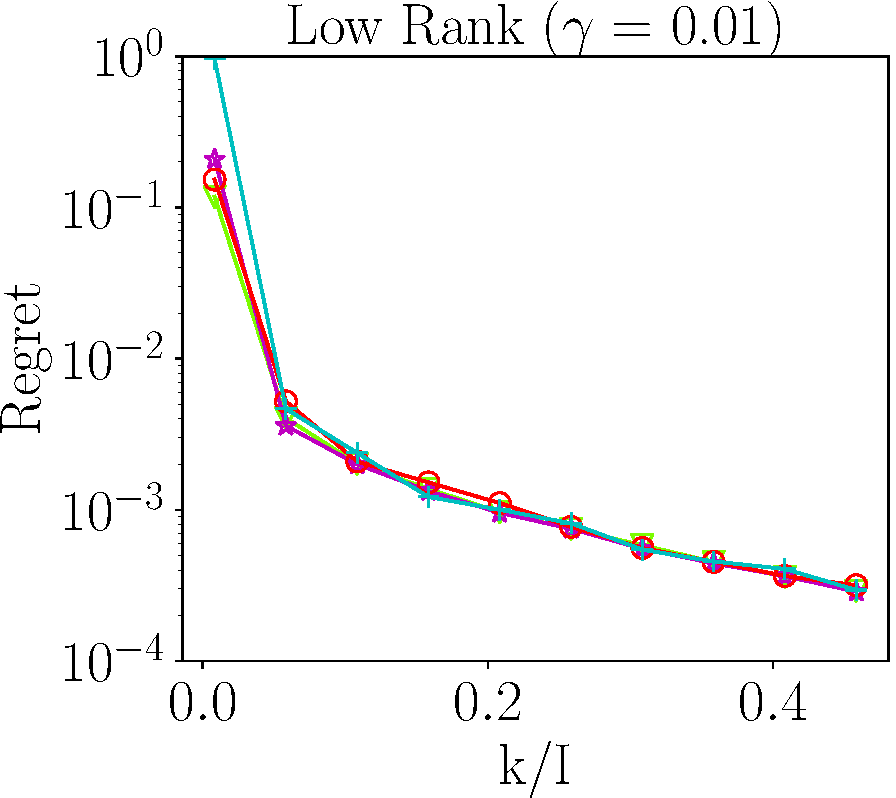
\includegraphics[scale = 0.24]{figure/fig2_lk_lnoise_600.pdf}
	\end{subfigure}
	\begin{subfigure}{0.3\textwidth}
		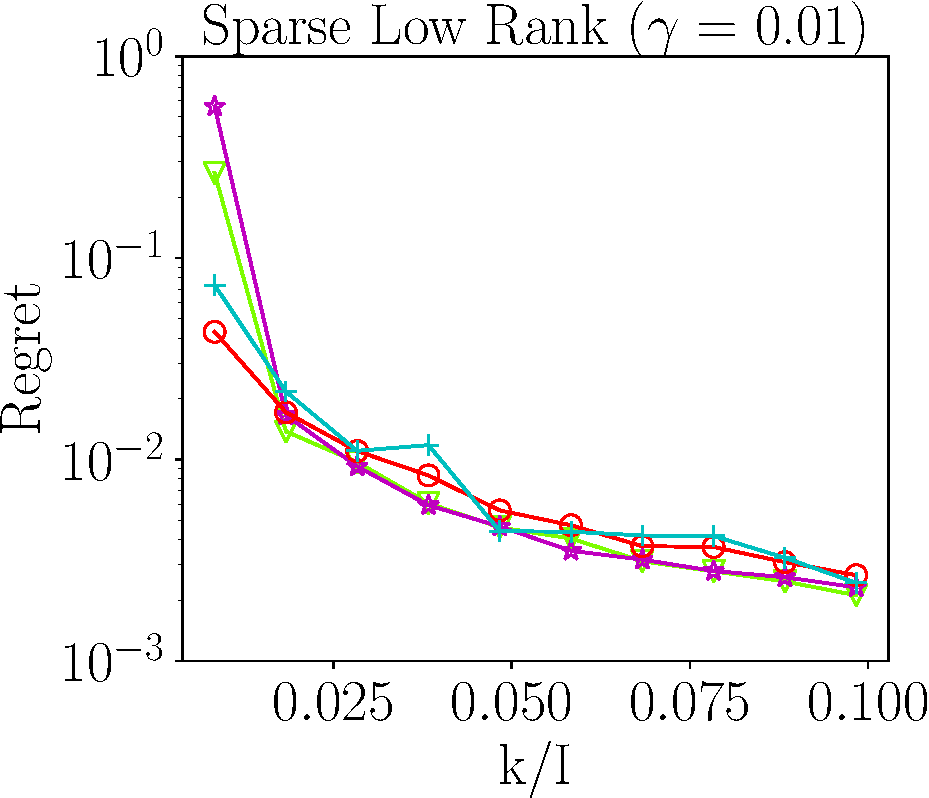
\includegraphics[scale = 0.24]{figure/fig2_slk_lnoise_600.pdf}
	\end{subfigure}
	\begin{subfigure}{0.3\textwidth}
		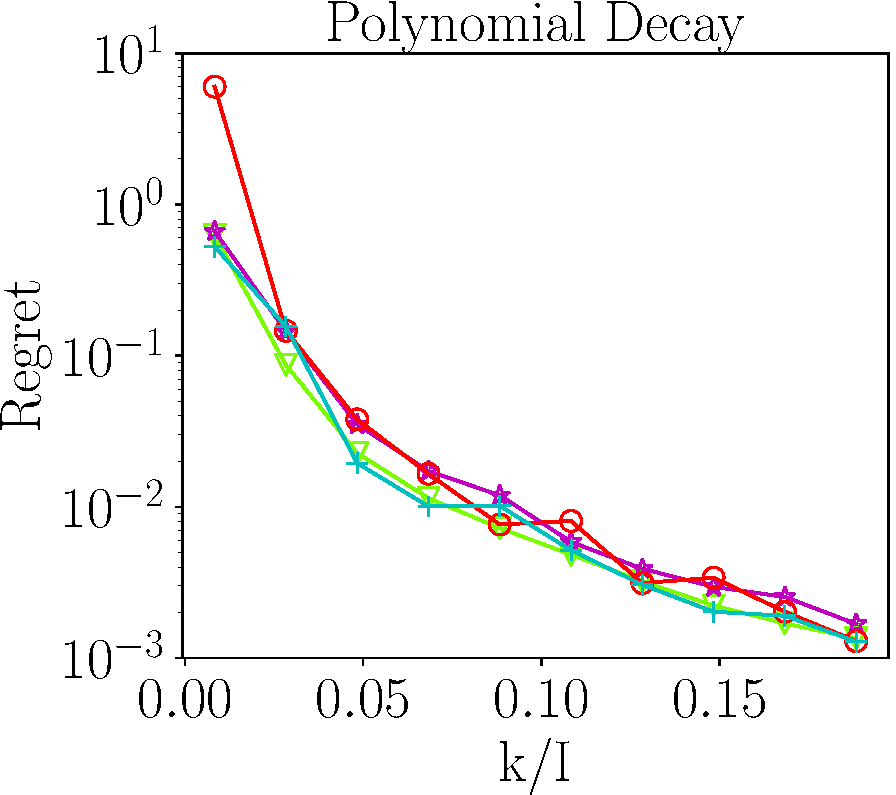
\includegraphics[scale = 0.24]{figure/fig2_spd_600.pdf}
	\end{subfigure}\\
	\begin{subfigure}{0.3\textwidth}
		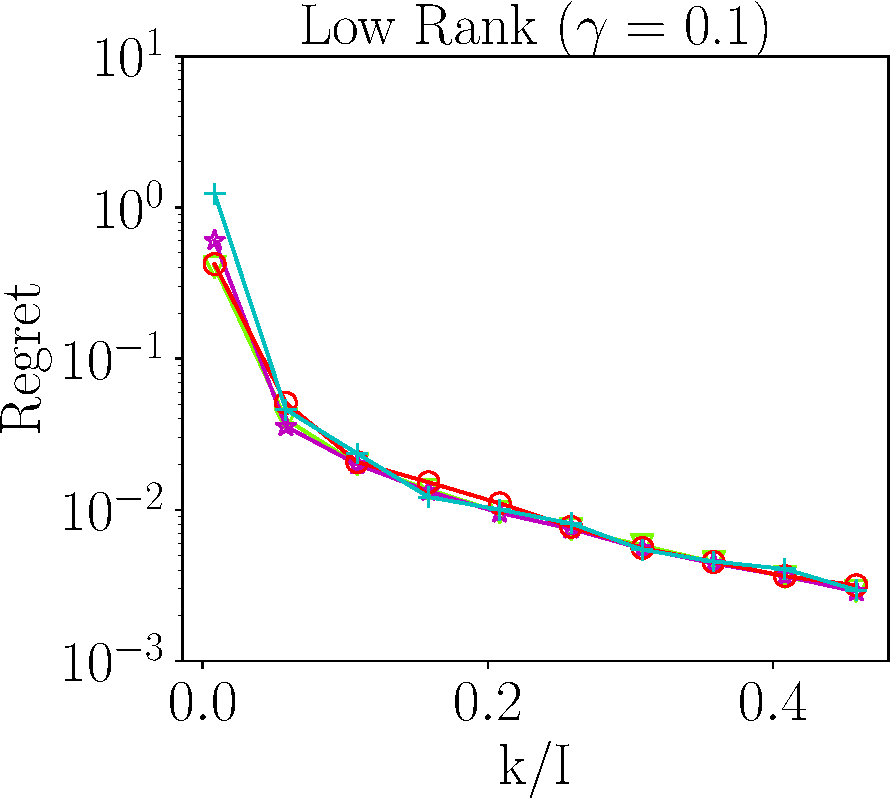
\includegraphics[scale = 0.24]{figure/fig2_lk_mnoise_600.pdf}
	\end{subfigure}
	\begin{subfigure}{0.5\textwidth}
		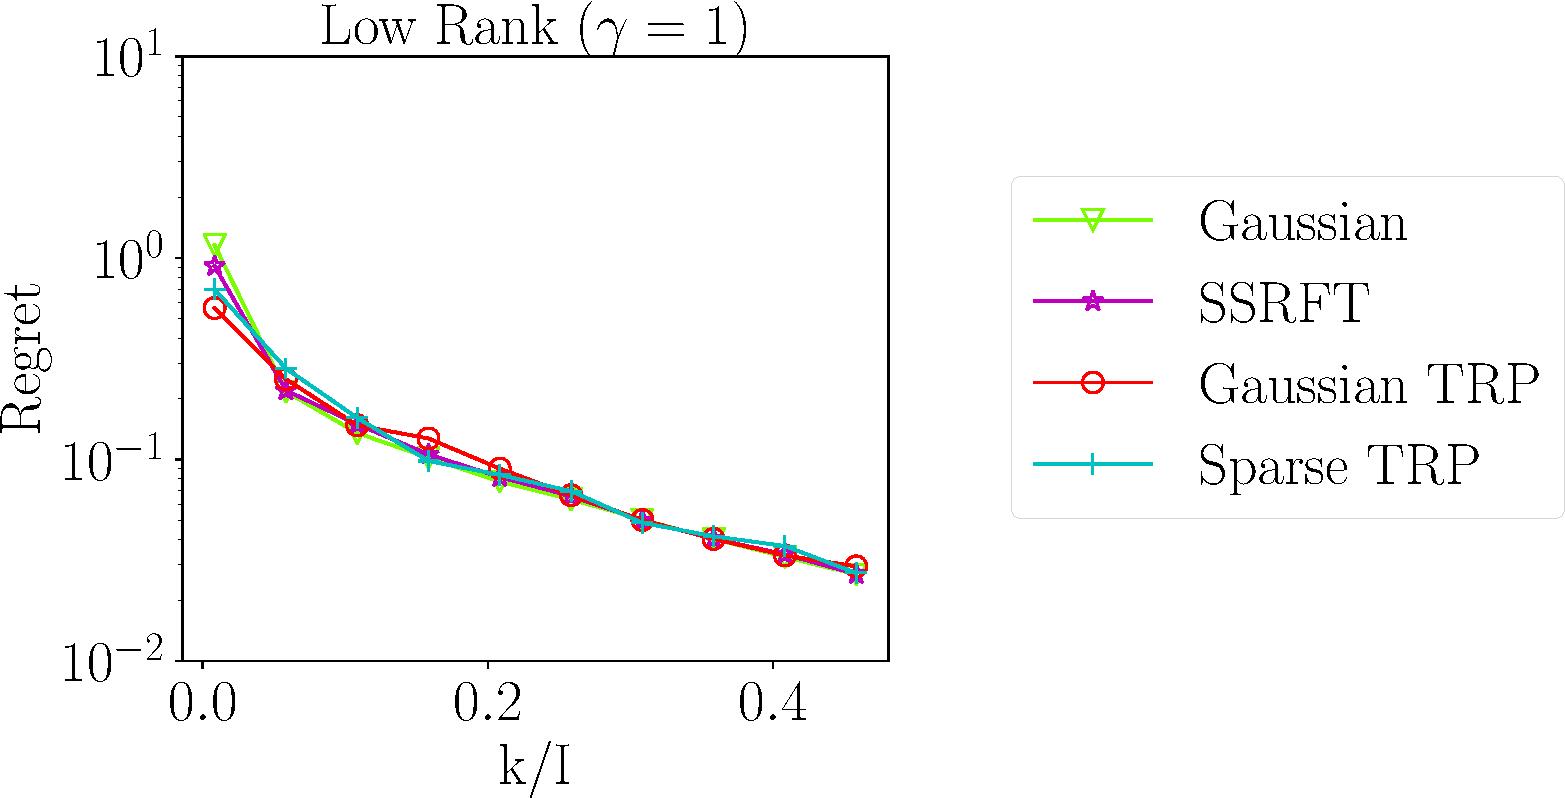
\includegraphics[scale = 0.24]{figure/fig2_lk_hnoise_600.pdf}
	\end{subfigure}
	\\
	\caption{\textit{Different DRMs perform similarly.}
		We approximate 3D synthetic tensors (see \ref{s-synthetic-data}) with $I = 600$,
		using our one-pass algorithm with $r = 5$ and varying $k$ ($s = 2k+1$),
		using a variety of DRMs in the Tucker sketch:
		Gaussian, SSRFT, Gaussian TRP, or Sparse TRP.
		\label{fig:vary-k-600}
	}
\end{figure}

\begin{figure}
	\centering
	\begin{subfigure}{0.3\textwidth}
		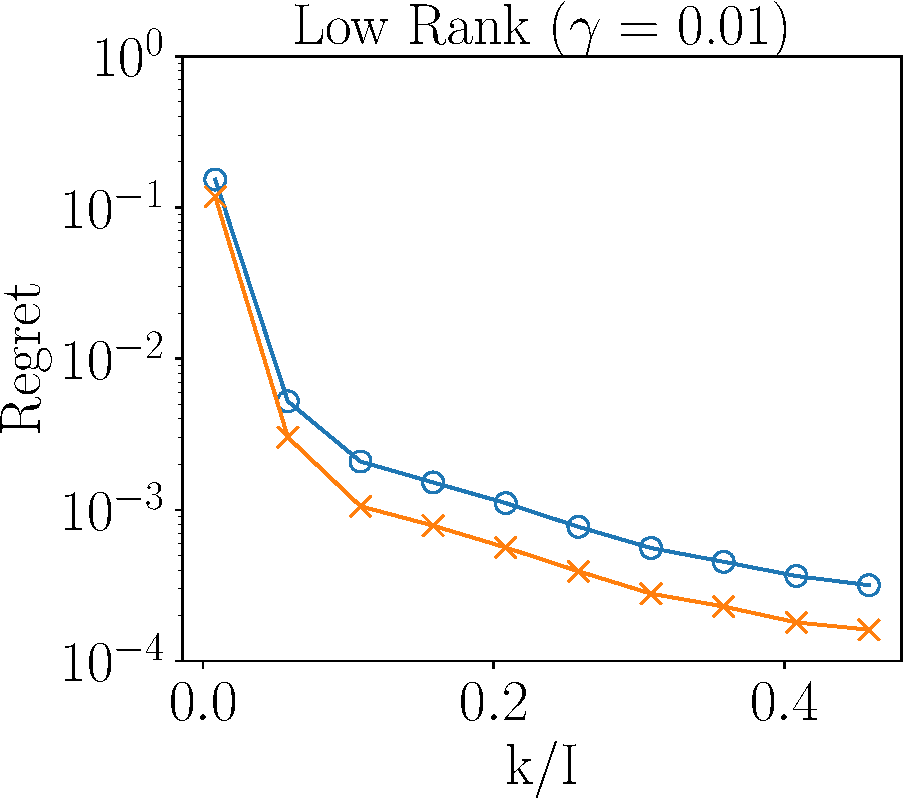
\includegraphics[scale = 0.24]{figure/fig3_lk_lnoise_600.pdf}
	\end{subfigure}
	\begin{subfigure}{0.3\textwidth}
		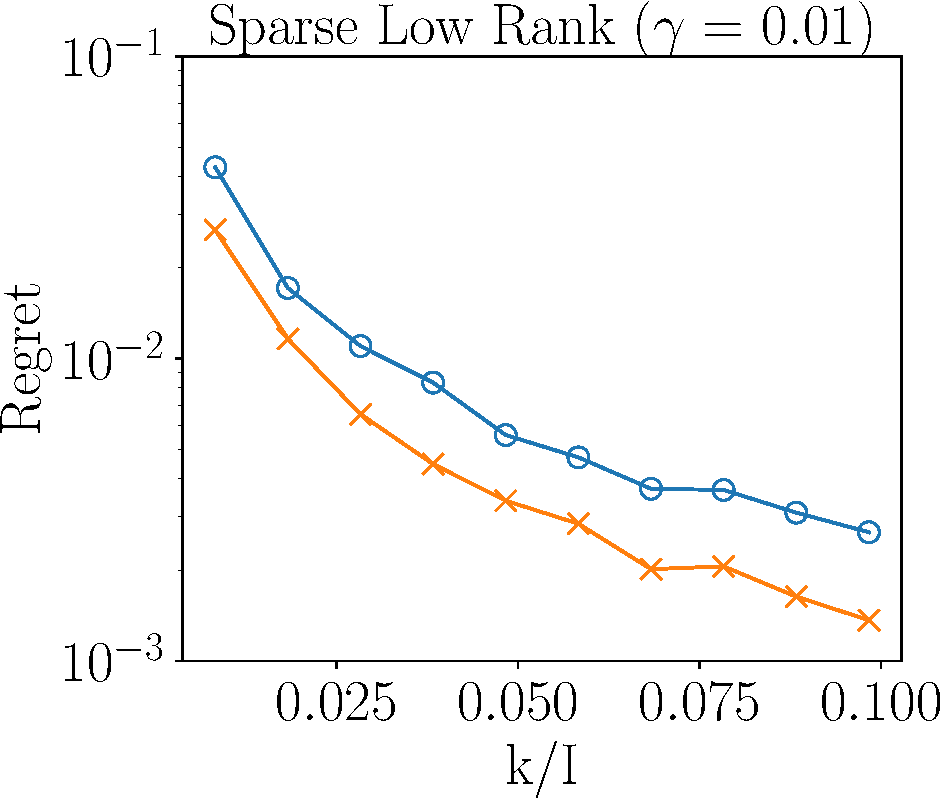
\includegraphics[scale = 0.24]{figure/fig3_slk_lnoise_600.pdf}
	\end{subfigure}
	\begin{subfigure}{0.3\textwidth}
		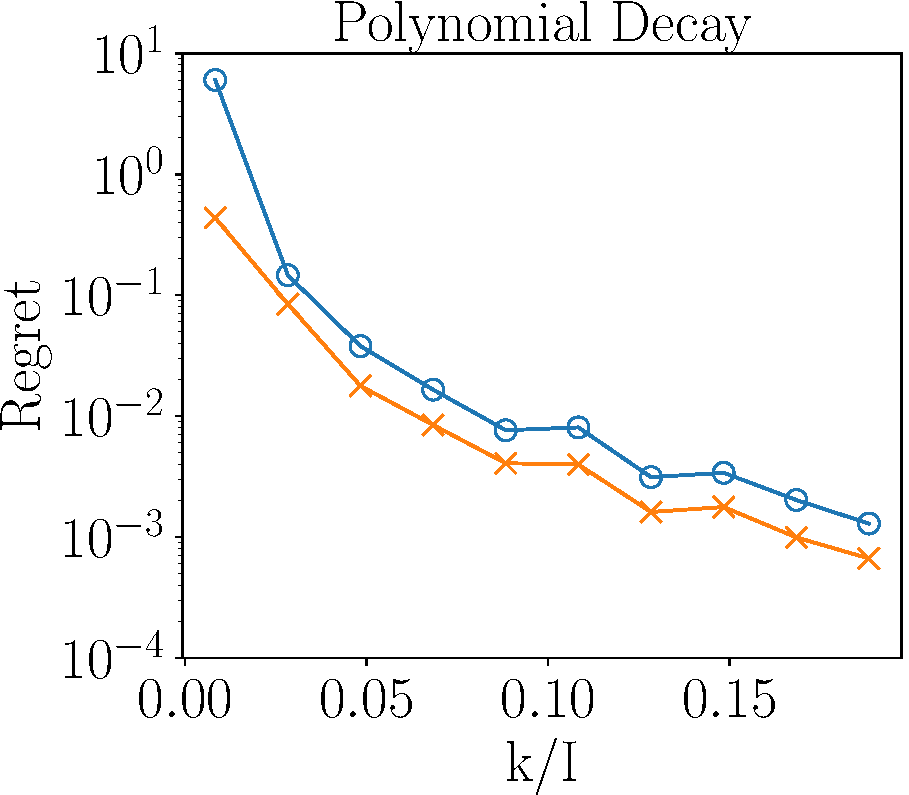
\includegraphics[scale = 0.24]{figure/fig3_spd_600.pdf}
	\end{subfigure}\\
	\begin{subfigure}{0.3\textwidth}
		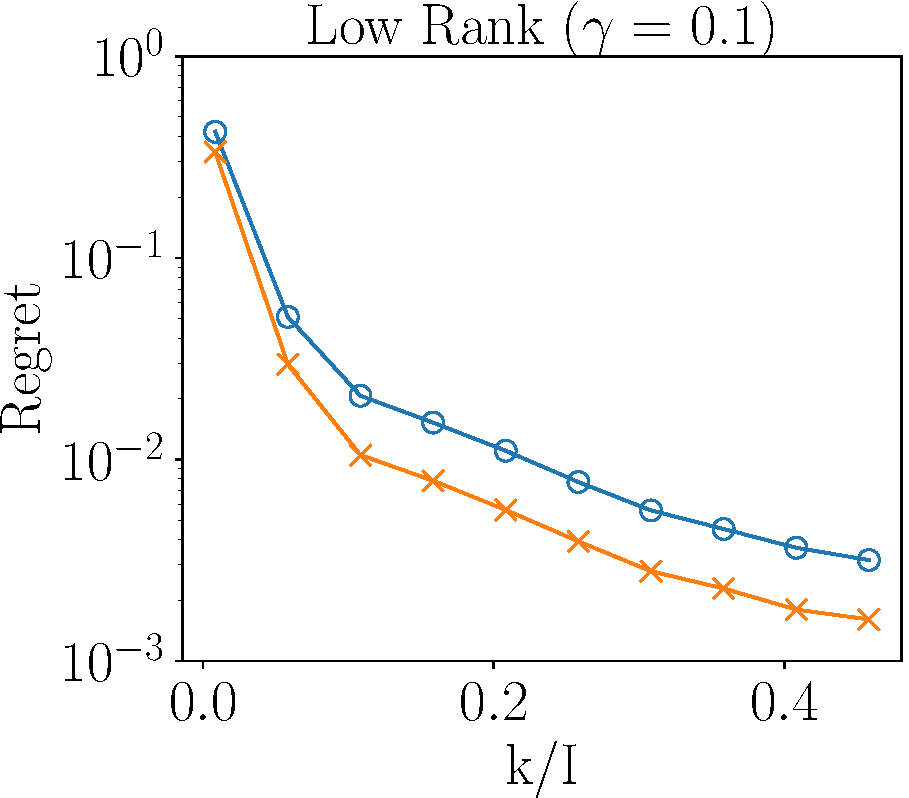
\includegraphics[scale = 0.24]{figure/fig3_lk_mnoise_600.pdf}
	\end{subfigure}
	\begin{subfigure}{0.55\textwidth}
		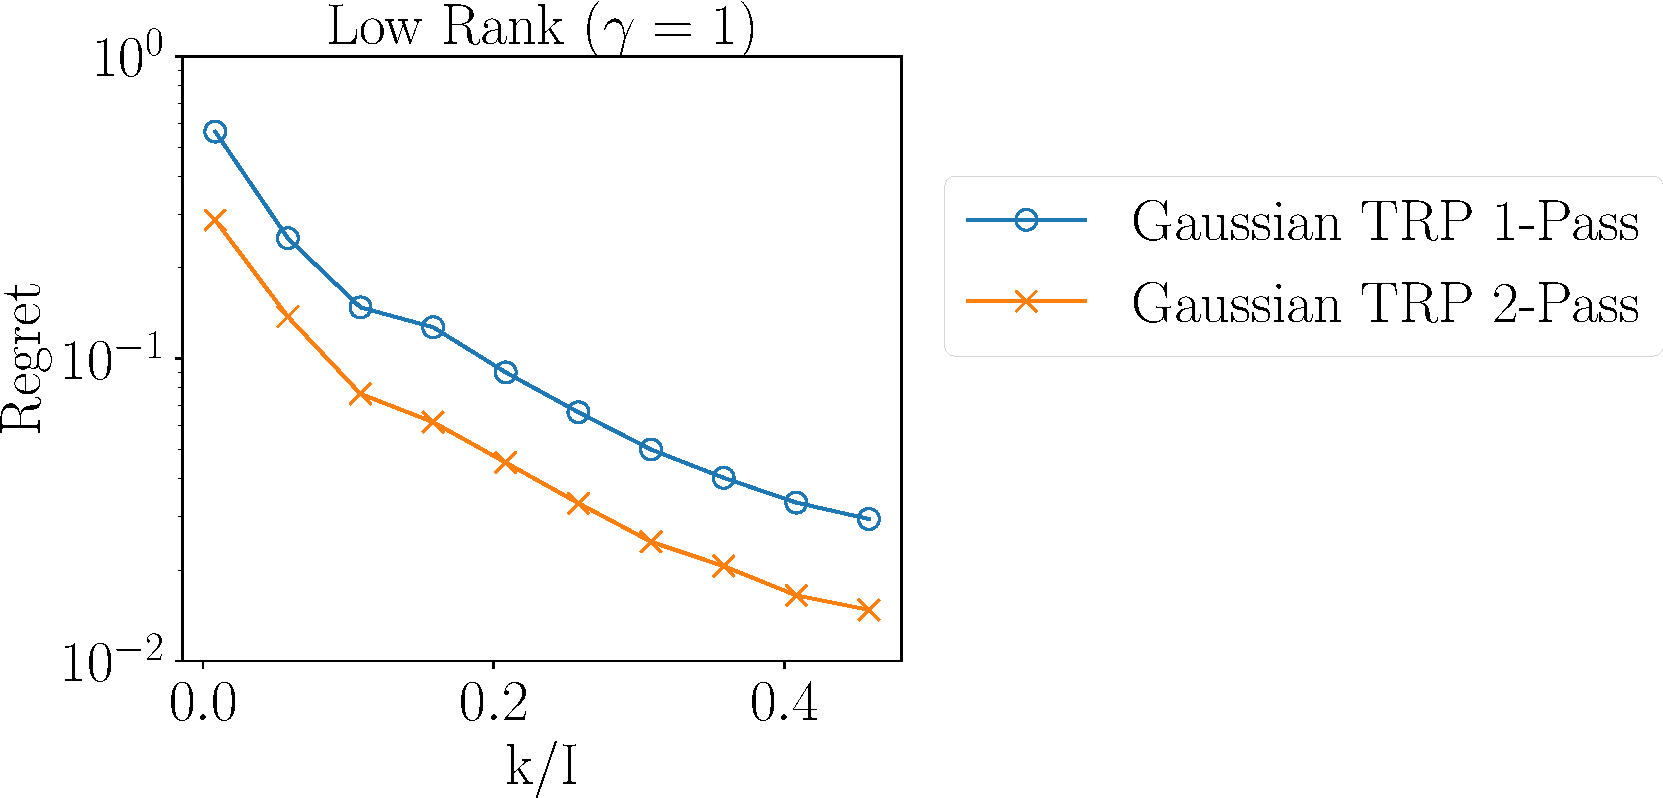
\includegraphics[scale = 0.24]{figure/fig3_lk_hnoise_600.pdf}
	\end{subfigure}
	\\
	\caption{\textit{Two-pass improves on one-pass.}
	We approximate 3D synthetic tensors (see \ref{s-synthetic-data}) with $I = 600$,
	using our one-pass and two-pass algorithms with $r = 5$ and varying $k$ ($s = 2k+1$),
	using the Gaussian TRP in the Tucker sketch.
	\label{fig:vary-k-600-compare}
  }
\end{figure}
In this section, we study the performance of our method.
We compare the performance of the method using various different
DRMs, including TRP.
We also compare our method with the algorithm proposed by \cite{malik2018low}
to show that for the same storage budget, our method produces better approximations.
Our two-pass algorithm outperforms the one-pass version, as expected.
(Contrast this to \cite{malik2018low}, where the multi-pass method
performs less well than the one-pass version.)
% Experiments on real data show effective compression
% can be achieved in a single pass.

\begin{figure}
	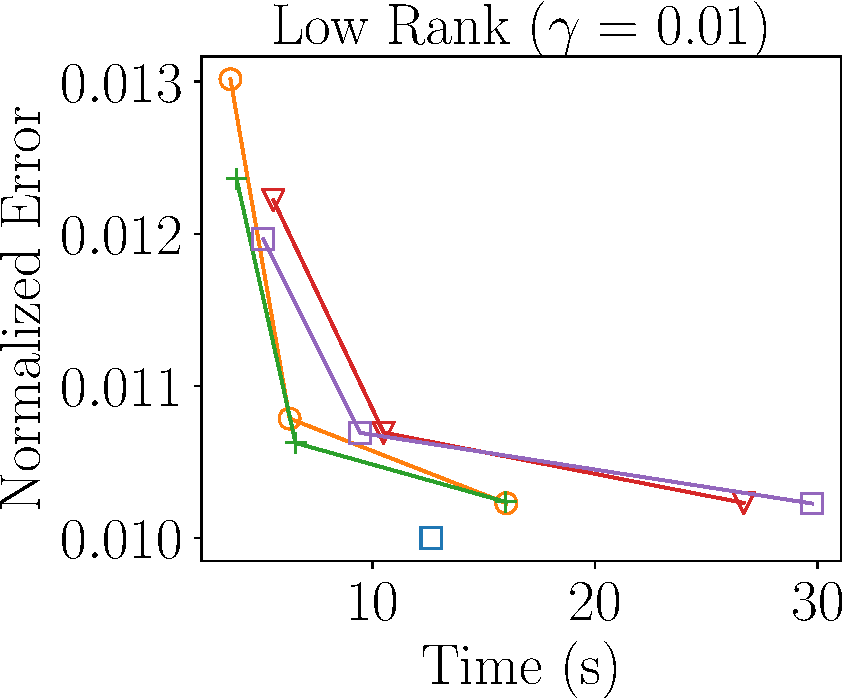
\includegraphics[height=2.5cm]{figure/lk_1pass_time.pdf}
	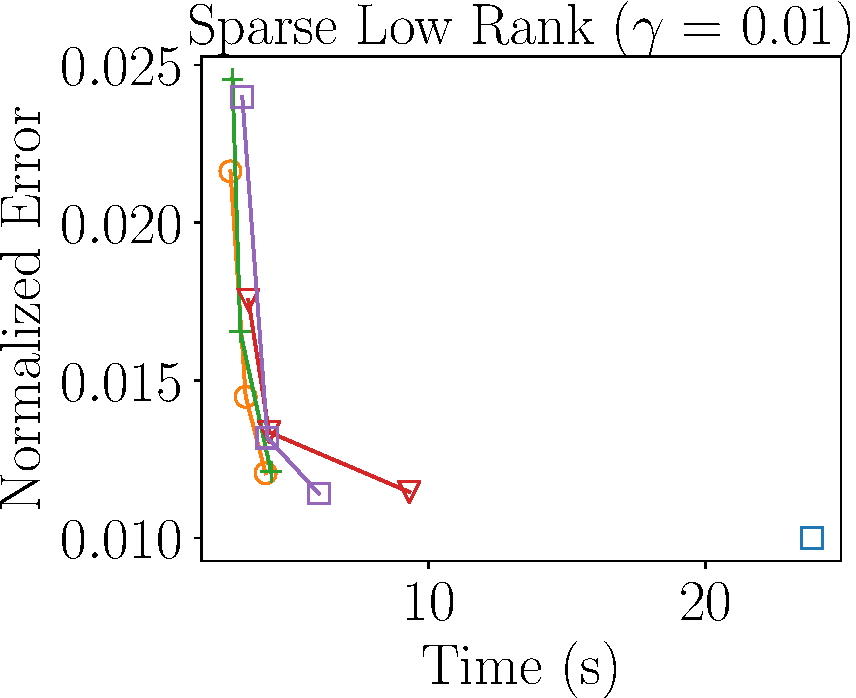
\includegraphics[height=2.5cm]{figure/slk_1pass_time.pdf}
	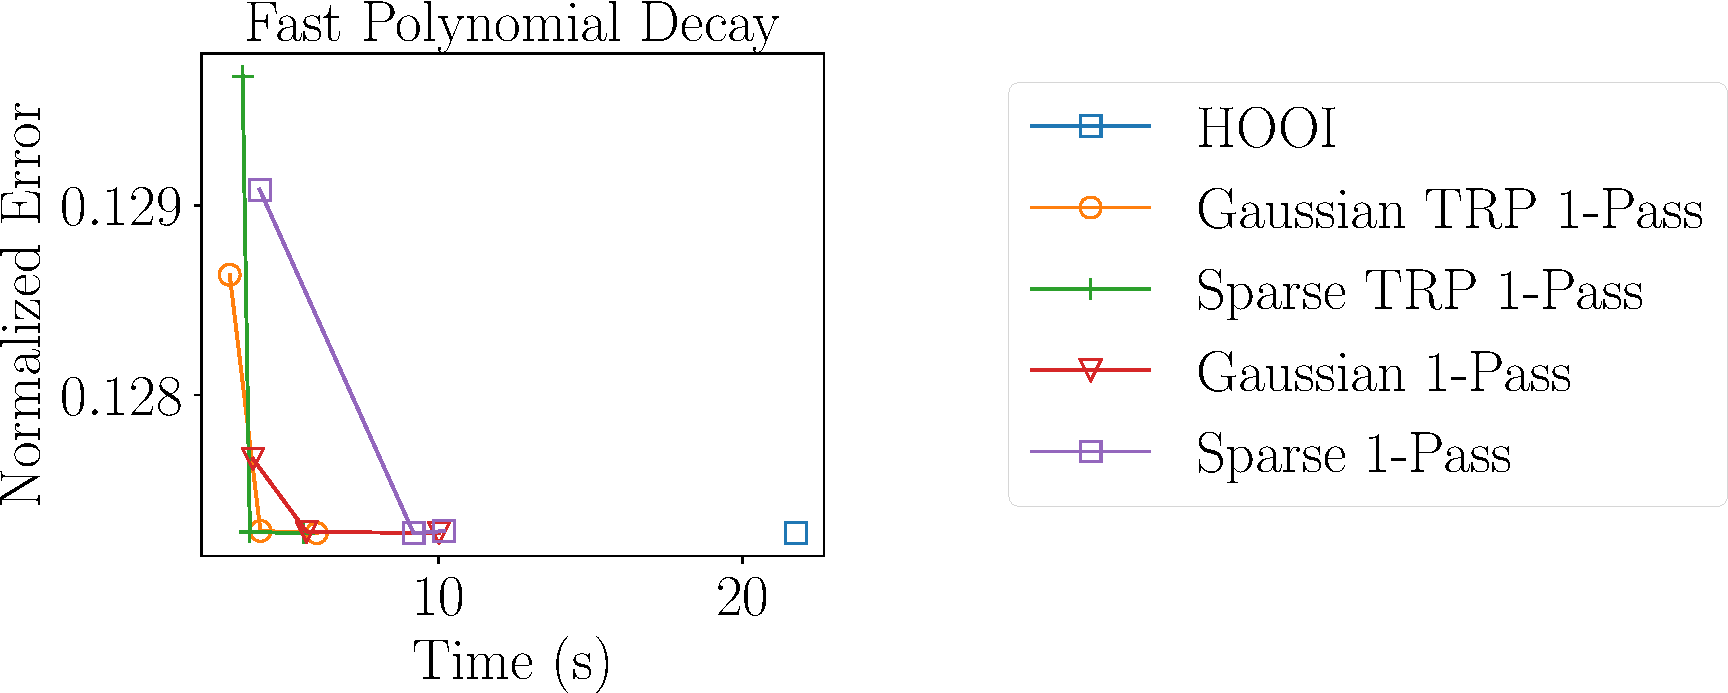
\includegraphics[height=2.5cm]{figure/fpd_1pass_time.pdf}\\
	\centering
	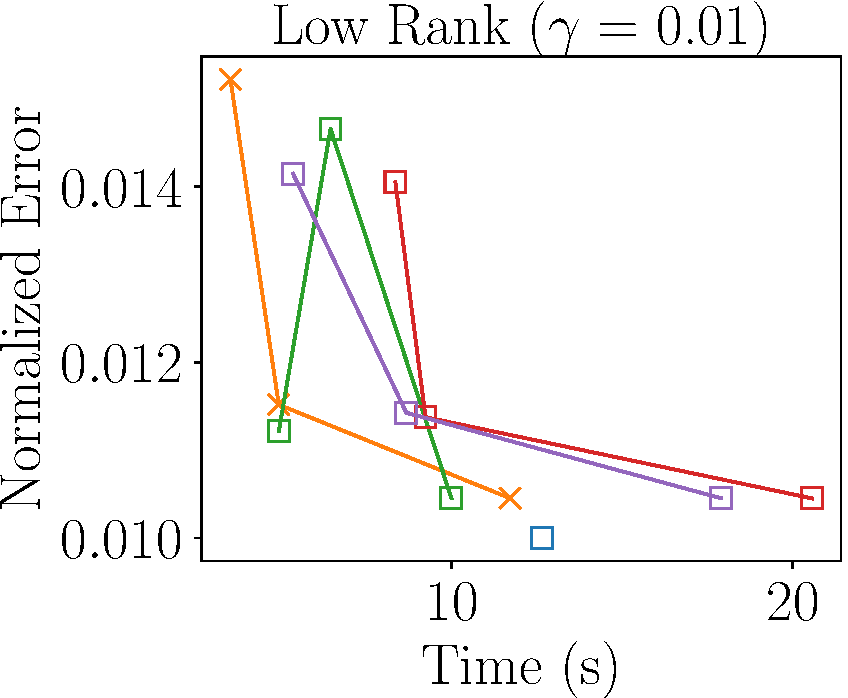
\includegraphics[height=2.5cm]{figure/lk_2pass_time.pdf}
	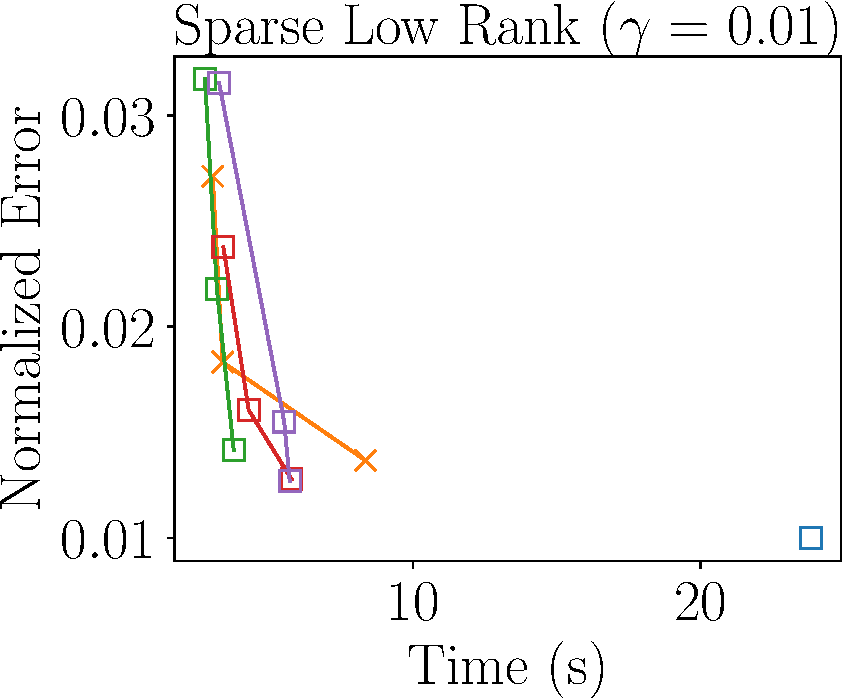
\includegraphics[height=2.5cm]{figure/slk_2pass_time.pdf}
	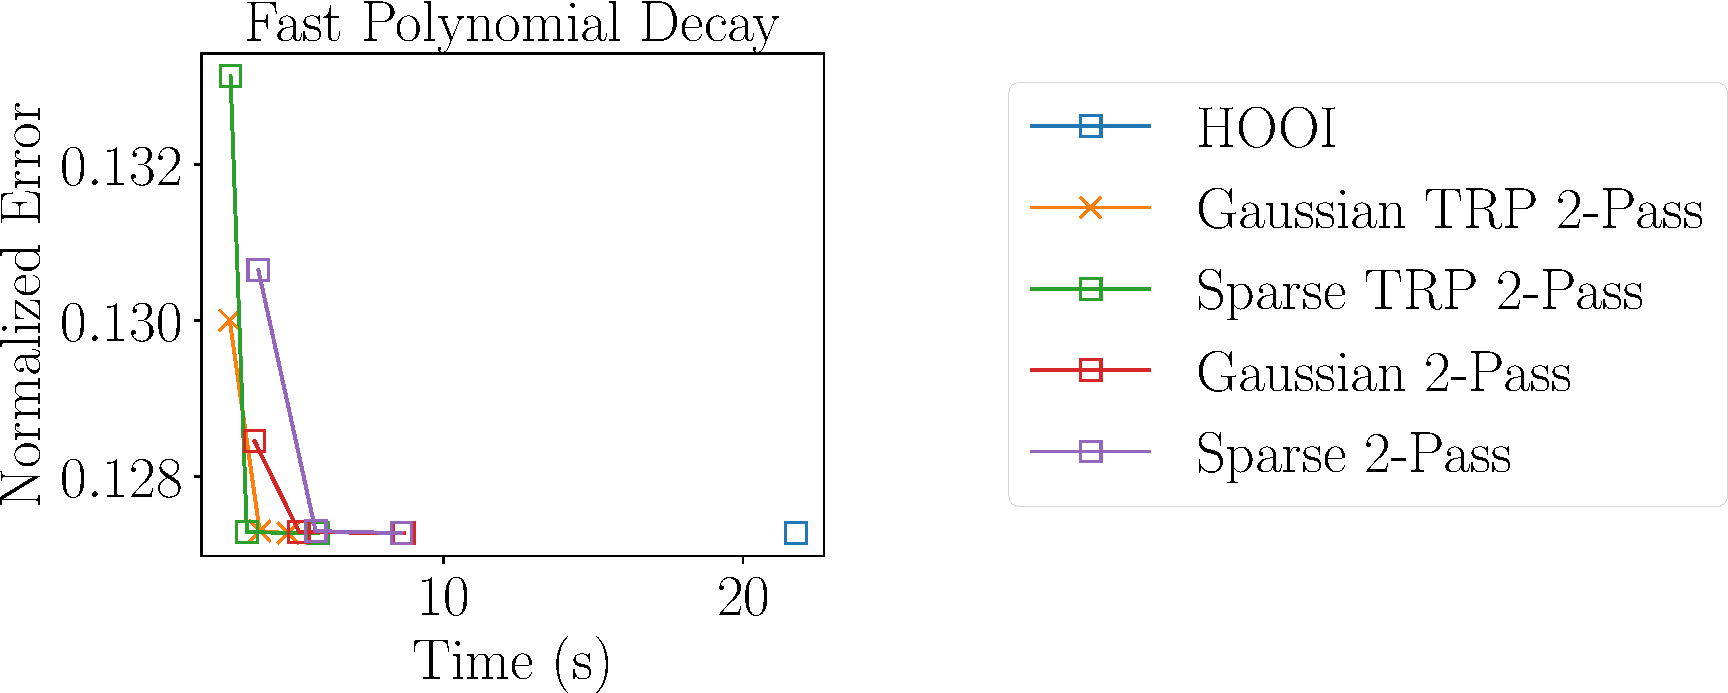
\includegraphics[height=2.5cm]{figure/fpd_2pass_time.pdf}\\
	\centering
	\caption{
	\textit{Faster approximations.}
	We approximate 3D synthetic tensors with $I = 600$ generated
	as described in \ref{s-synthetic-data},
	using HOOI and our one-pass and two-pass algorithms with $r = 5$
	for a few different $k$ ($s = 2k+1$).
	% We try several DRMs in the Tucker sketch:
	% Gaussian, Sparse, Gaussian TRP, and Sparse TRP.
	% Tradeoff between Time and Relative Error: We compare HOOI and our two algorithms across different random maps with $I=600, \mathbf{r}=(5,5,5)$, $\gamma = 0.01$.
}\label{fig:run_time}
\end{figure}

We evaluate the experimental results using two metrics:
\[
% \begin{array}{lc}
% \mbox{normalized error:} & \frac{\|\T{X} - \hat{\T{X}}\|_F}{\|\T{X}\|_F} \\
% \mbox{relative error:} & \frac{\|\T{X} - \hat{\T{X}}\|}{\|\T{X} - \T{X}_\text{HOOI}\|} - 1 \\
% \mbox{regret:} & \frac{\|\T{X} - \hat{\T{X}}\|_F}{\|\T{X}\|_F} -
%                    \frac{\|\T{X} - \T{X}_\text{HOOI}\|_F}{\|\T{X}\|_F}.
% \end{array}
\begin{array}{lc}
\mbox{normalized error:} & \|\T{X} - \hat{\T{X}}\|_F / \|\T{X}\|_F \\
% \mbox{relative error:} & \nicefrac{\|\T{X} - \hat{\T{X}}\|}{\|\T{X} - \T{X}_\text{HOOI}\|} - 1 \\
\mbox{regret:} & \left(\|\T{X} - \hat{\T{X}}\|_F - \|\T{X} - \T{X}_\text{HOOI}\|_F \right) / \|\T{X}\|_F.
\end{array}
\]
The normalized error measures the fraction of the energy in $\T{X}$
captured by the approximation.
The regret measures the increase in normalized error due to
using the approximation $\hat{\T{X}}$ rather than using $\T{X}_\text{HOOI}$.
The relative error measures the decrease in performance relative to HOOI.
%\mnote{Joel says: I prefer to call this the "normalized" error, rather than the "relative" error. The former scales the error so it should usually be less than one. The second compares the error with the "optimum" error: ||X - hat{X}|| / ||X - HOOI(X)|| - 1.You might consider whether you actually want the latter.}
The normalized error of a rank $\V{r}$ Tucker approximation $\hat{X}$
is always positive when $\T{X}$ has a larger rank.
In general, we find our proposed methods approaches the performance of HOOI
for large enough storage budgets.

We ran all experiments on a server with 128 Intel\textsuperscript{\textregistered} Xeon\textsuperscript{\textregistered} E7-4850 v4 2.10GHz CPU cores and 1056GB memory.
The code for our method is available at an anonymous Github repository \url{https://github.com/tensorsketch/tensorsketch}.

\subsection{Synthetic experiments}\label{s-synthetic-data}
All synthetic experiments use an input tensor with equal side lengths $I$.
We consider three different data generation schemes:
\begin{itemize}
\item \emph{Low rank + noise.} Generate a core tensor $\T{C} \in \mathbb{R}^{r^N}$ with entries drawn from $\mathrm{Unif}([0,1])$.
  Independently generate $N$ orthogonal factor matrices
  $\mathbf{A}_1, \dots, \mathbf{A}_N \in \mathbb{R}^{r \times I}$.
	Define $\T{X}^\natural = \T{C} \times_1 \mathbf{A}_1 \cdots \times_N \mathbf{A}_N$
	and the noise parameter $\gamma > 0$.
	Generate an input tensor as
	$\T{X} = \T{X}^\natural + (\gamma \|\T{X}^\natural\|_F / I^{N/2})\T{\epsilon}$
	where the noise $\T{\epsilon}$ has i.i.d. $\mathcal{N}(0,1)$ entries.
	% by orthogonalizing random matrices with each entry drawn from $\mathcal{N}(0,1)$.
%   The input tensor is
%  \[
% \T{X} = \T{C} \times_1 \mathbf{A}_1 \cdots \times_N \mathbf{A}_N + \sqrt{\frac{\gamma^2 \cdot \|\T{X}^\natural\|_F^2}{I^N}} \mathcal{N}(0,1),
% \]
% where $\T{X}^\natural = \T{C} \times_1 \mathbf{A}_1 \cdots \times_N \mathbf{A}_N$.
% Here $1/\gamma^2$ measures the signal-to-noise ratio.
% In the simulations, we use three different noise levels: $\gamma = 0.01, 0.1, 1$.
\item \emph{Sparse low rank + noise.} We construct the input tensor $\T{X}$ as above (Low Rank + Noise),
but with sparse factor matrices $\mathbf{A}_n$:
If $\delta_n$ is the sparsity (proportion of non-zero elements) of $\mathbf{A}_n$,
then the sparsity of the true signal $\T{X}^\natural$ is $\prod_{n=1}^N \delta_n$.
%We set the noise $\gamma = 0.01$ (Results for $\gamma = 0.1,0.1$ are empirically analogous to the previous setting).
We use $\delta_n = 0.2$ unless otherwise specified.
\item \emph{Polynomial decay.} We construct the input tensor $\T{X}$ as
  \begin{equation*}
      \T{X} = \mathop{\textbf{superdiag}}(1,\dots,1, 2^{-t},3^{-t},\dots, (I-r)^{-t}).
  \end{equation*}
  The first $r$ entries are 1.
	Recall $\mathop{\textbf{superdiag}}$ converts a vector to $N$ dimensional superdiagonal tensor.
  Our experiments use $t = 1$ (geometric decay).
\end{itemize}

\subsubsection{Different dimension reduction maps perform similarly}
Our first experiment investigates the performance of our one-pass fixed-rank algorithm
as the sketch size (and hence, required storage) varies,
for several types of dimension reductions maps, including Gaussian, SSRFT, Gaussian TRP, and Sparse TRP.
We generate synthetic data as described above with $\mathbf{r} = (5,5,5), I = 600$.
\ref{fig:vary-k-600} shows the rank-$\mathbf{r}$ approximation error
as a function of the compression factor $k/I$.
\ifdefined \issupplement
(Results for other input tensors appear in the supplement.)
\else
(Results for other input tensors are presented as
\ref{fig:vary-k-400-app} and \ref{fig:vary-k-200-app} in \ref{appendix:more_result}.)
\fi
We see that the log relative error for our one-pass algorithm
converges to that of HOOI as $k$ increases for all input tensors.
In the low rank case, the convergence rate is lower for higher noise levels.
In general, the performance for different maps are approximately the same,
although our theory only pertains to the Gaussian map.
% In the low-rank sparse case and low-rank high noise case,
% the Gaussian TRP outperforms the Gaussian, possibly due to the implicit bias from the Khatri-Rao structure.

We evaluate the run time for HOOI and our two algorithms with several different DRMs in \ref{fig:run_time}. We can see that the one-pass algorithm is always slightly faster than the two-pass algorithm. The TRP generally provides a modest speedup in addition to the memory advantage.
Both our one-pass and two-pass algorithms achieve nearly the accuracy of HOOI,
and are usually much faster. % for tensors that are not exactly low rank.

\begin{figure}
	\centering
	\begin{subfigure}{0.3\textwidth}
		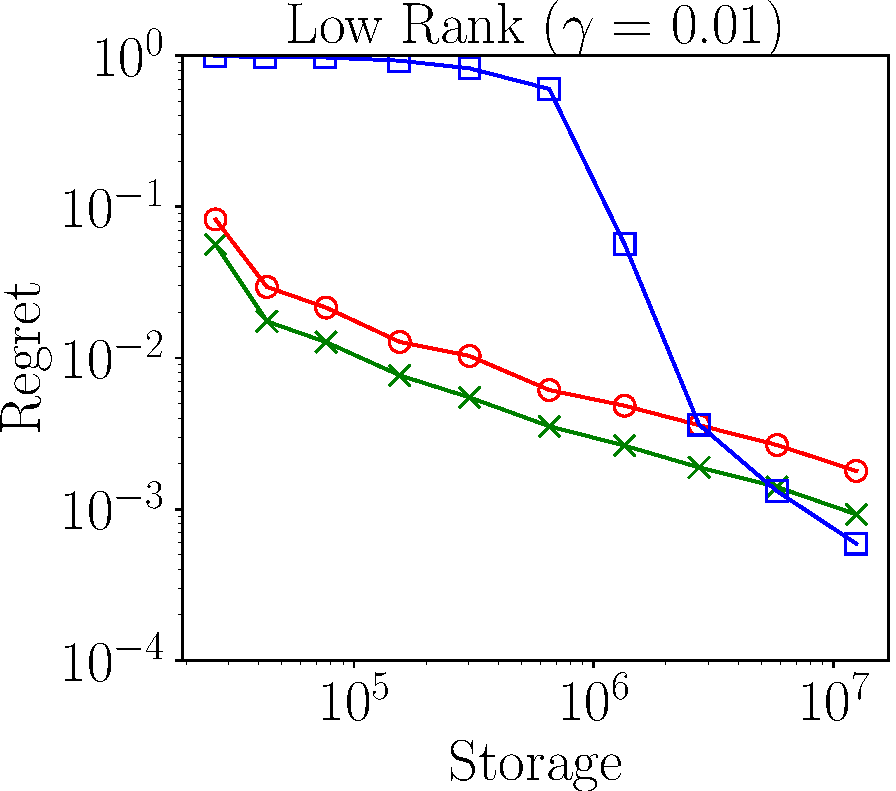
\includegraphics[scale = 0.24]{figure/fig1_lk_lnoise.pdf}
	\end{subfigure}
	\begin{subfigure}{0.3\textwidth}
		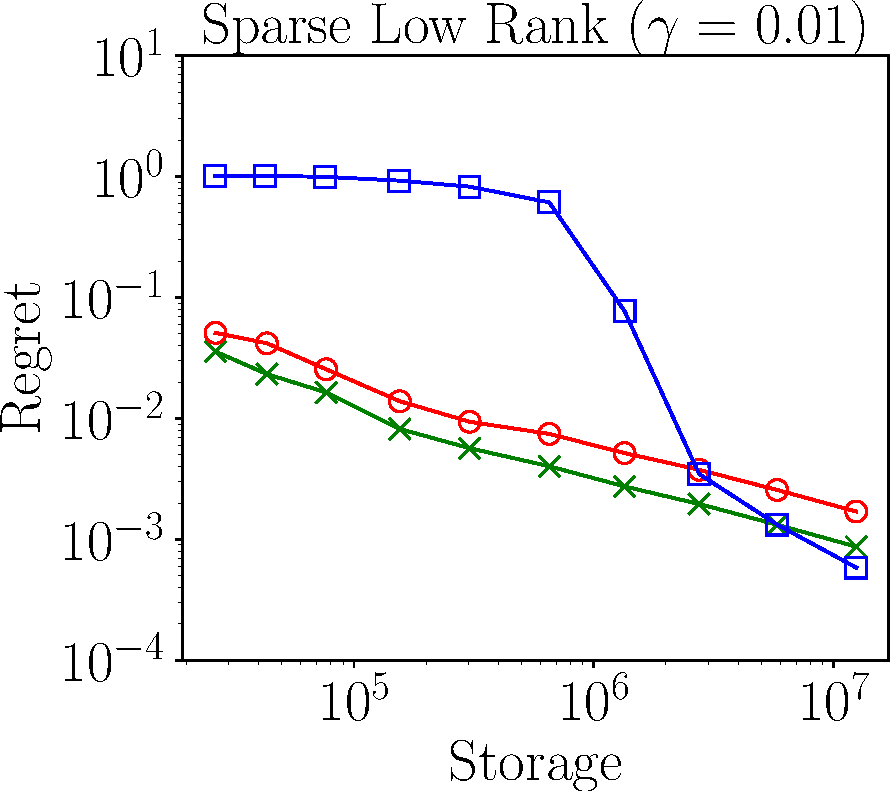
\includegraphics[scale = 0.24]{figure/fig1_slk_lnoise.pdf}
	\end{subfigure}
	\begin{subfigure}{0.3\textwidth}
		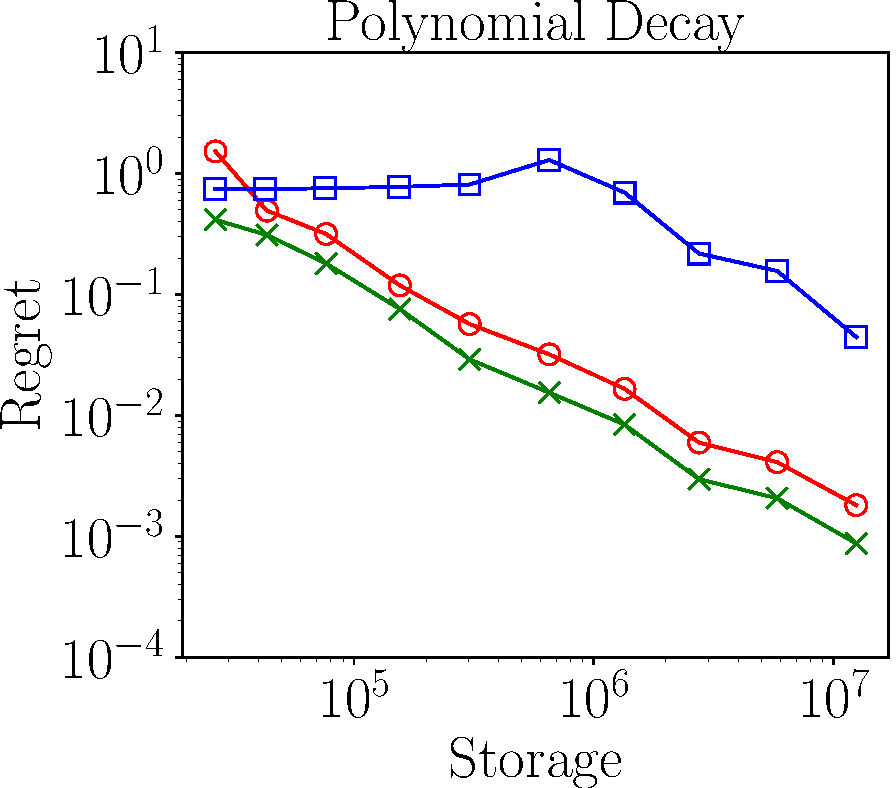
\includegraphics[scale = 0.24]{figure/fig1_spd.pdf}
	\end{subfigure}\\
	\begin{subfigure}{0.3\textwidth}
		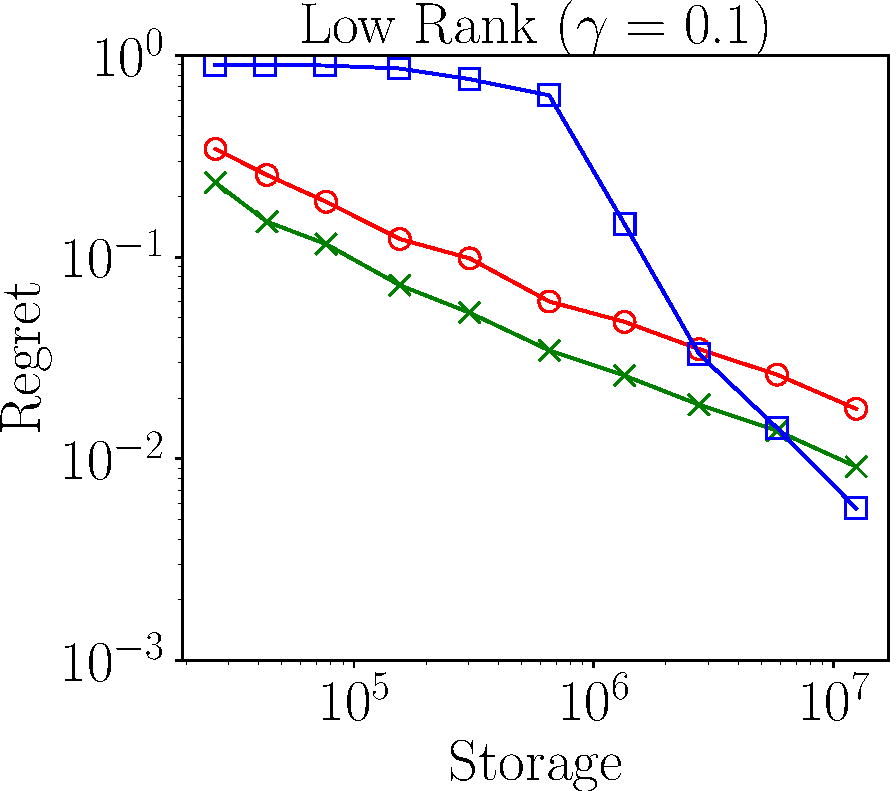
\includegraphics[scale = 0.24]{figure/fig1_lk_mnoise.pdf}
	\end{subfigure}
	\begin{subfigure}{0.43\textwidth}
		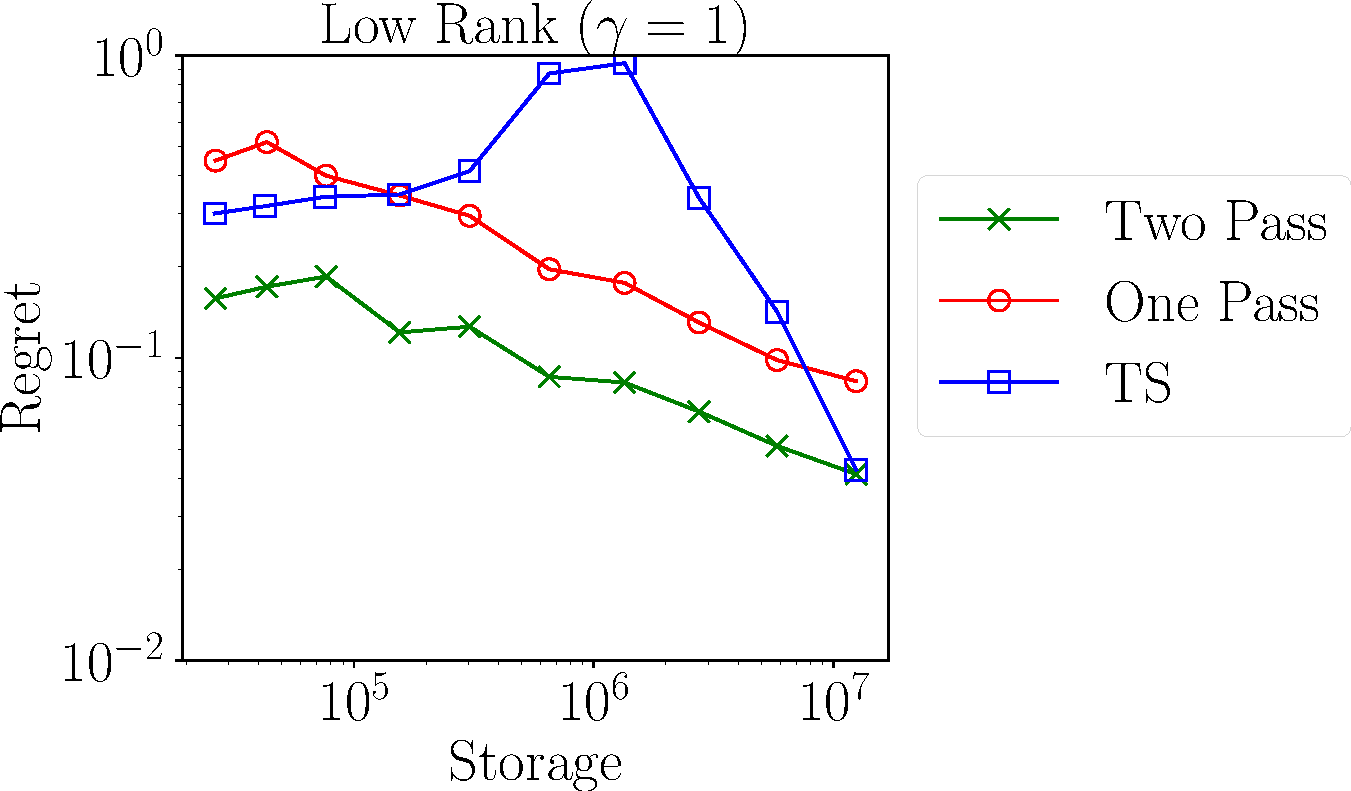
\includegraphics[scale = 0.24]{figure/fig1_lk_hnoise.pdf}
	\end{subfigure}\\
	\caption{\textit{Approximations improve with more memory: synthetic data.}
	We approximate 3D synthetic tensors (see \ref{s-synthetic-data}) with $I = 300$,
	using  T.-TS and our one-pass and two-pass algorithms
	with the Gaussian TRP to produce approximations with equal ranks $r=10$.
	Notice every marker on the plot corresponds to a 2700$\times$ compression!}\label{fig:vary-memory}
	% The total memory use is determined by the sketch size,
	% computed as $((2k+1)^N + kIN)$ for the one-pass method and $(Kr^{2N}+Kr^{2N-2})$ for T.-TS.
\end{figure}

\begin{figure}
	\centering
	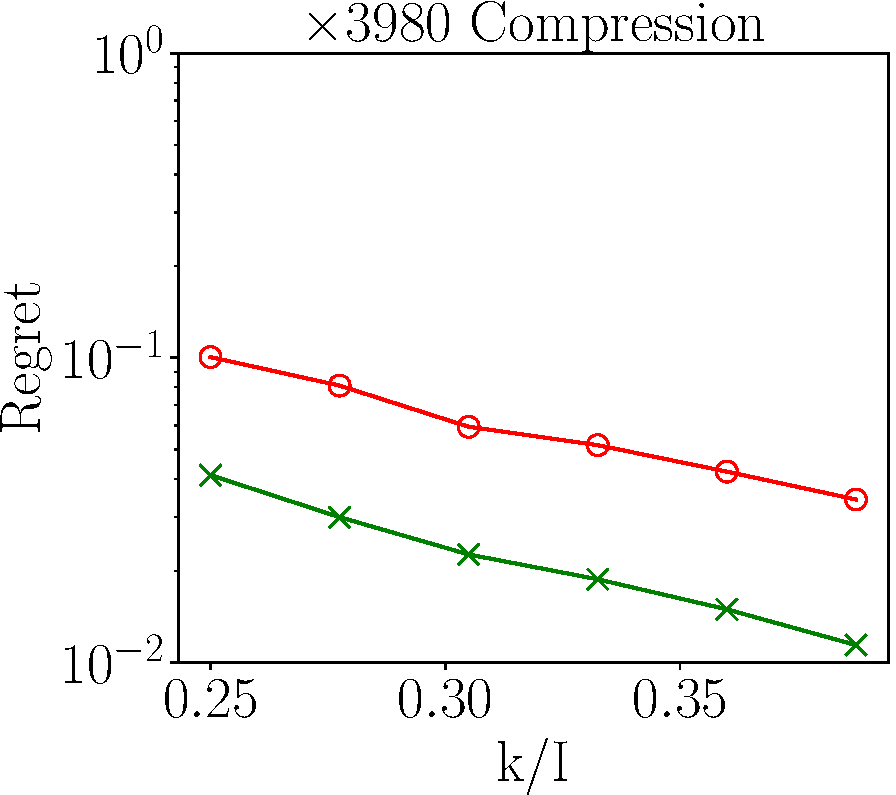
\includegraphics[height=2.9cm]{figure/multi_ABSORB_frk8.pdf}
	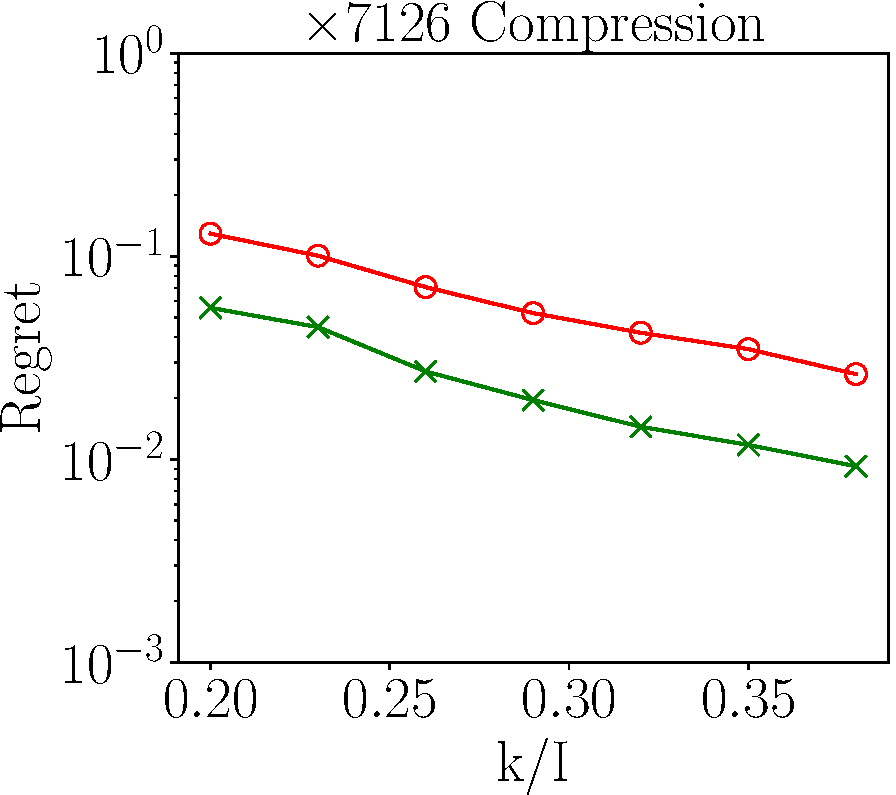
\includegraphics[height=2.9cm]{figure/multi_ABSORB_frk10.pdf}
	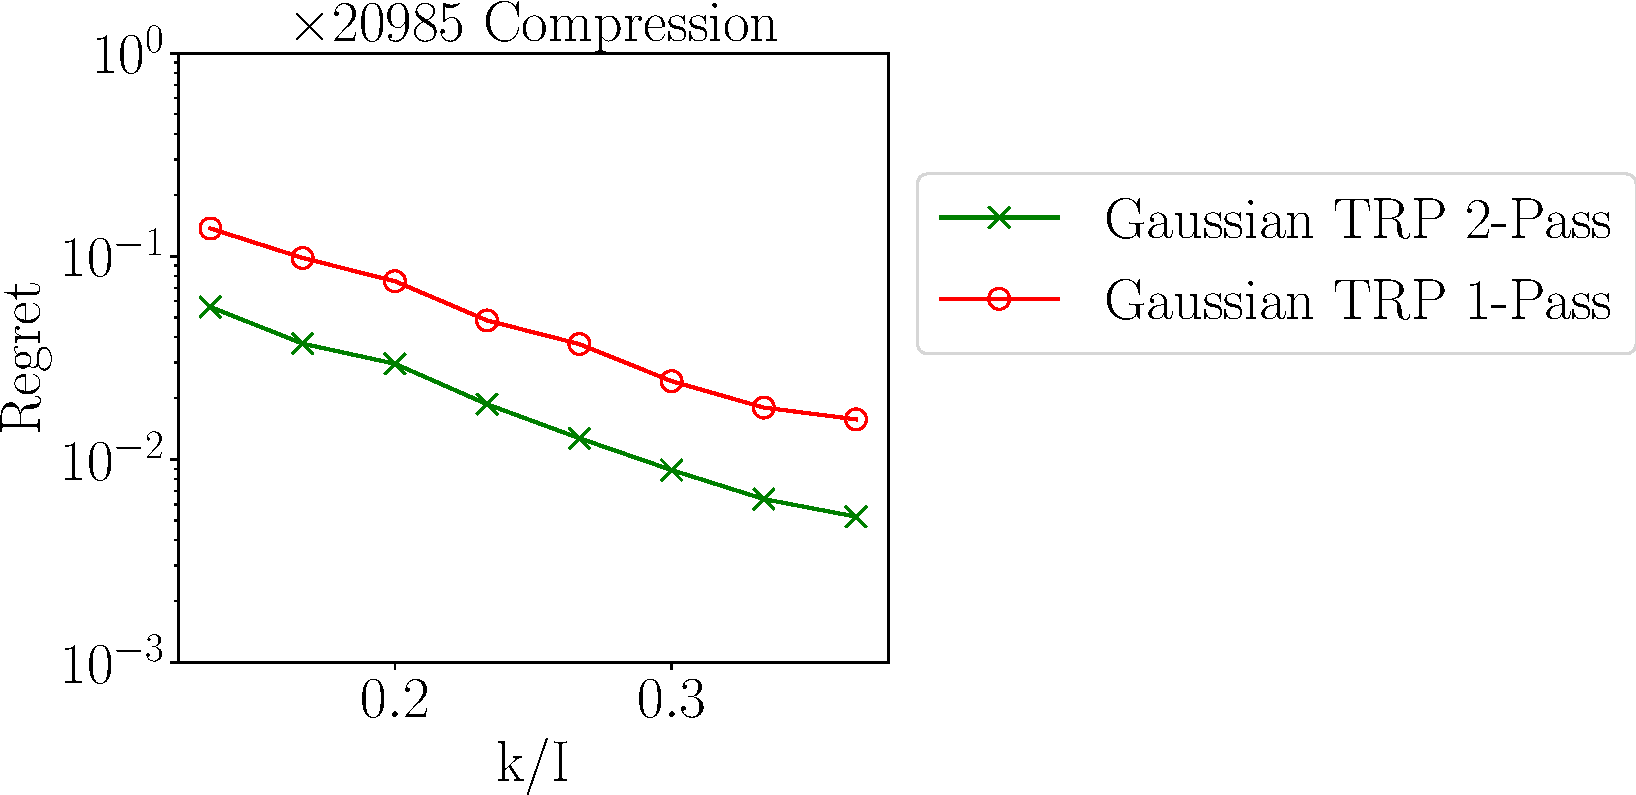
\includegraphics[height=2.9cm]{figure/multi_ABSORB_frk15.pdf}\\
	\textbf{Aerosol Absorption}\\~\\
	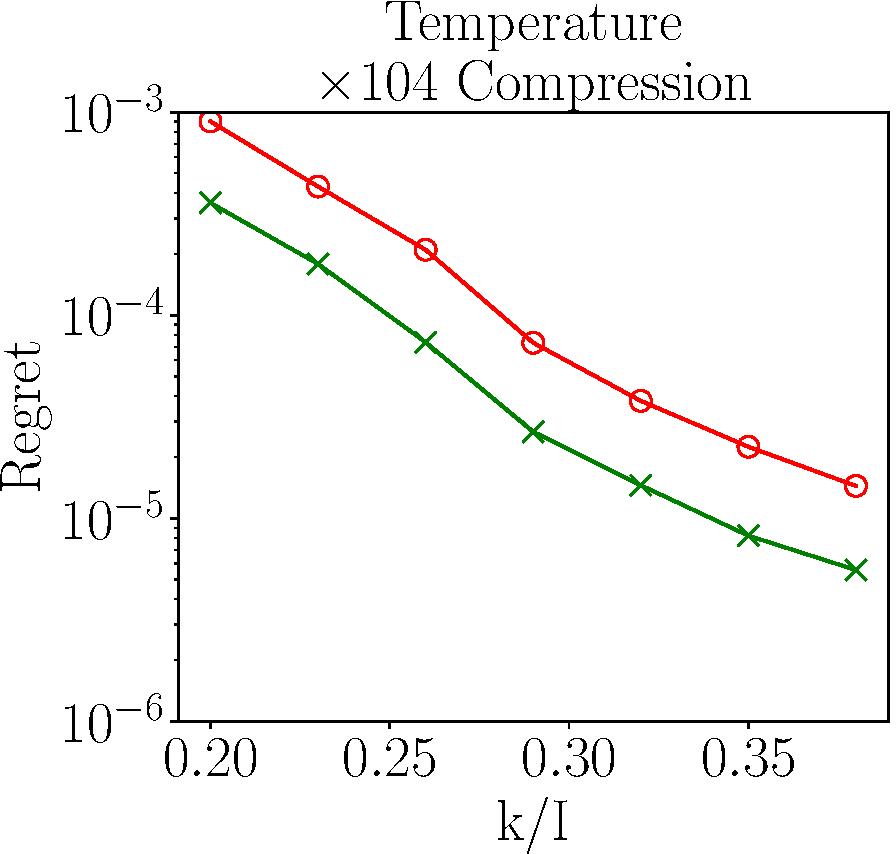
\includegraphics[height=2.9cm]{figure/multi_T_frk10.pdf}
	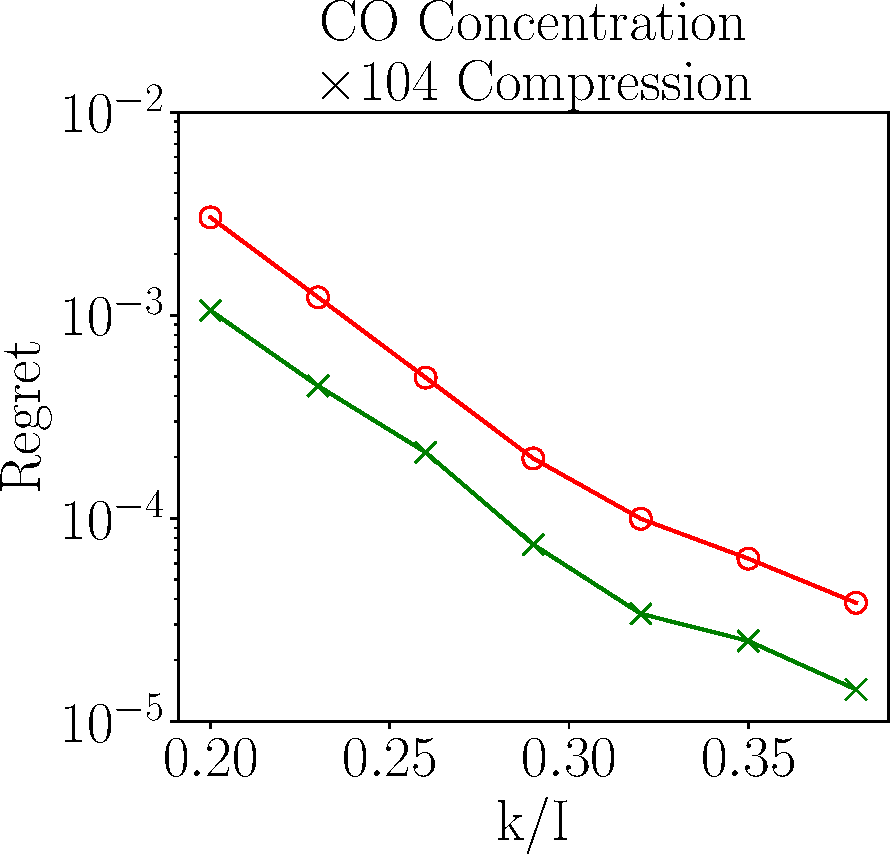
\includegraphics[height=2.9cm]{figure/multi_CO_frk10.pdf}
	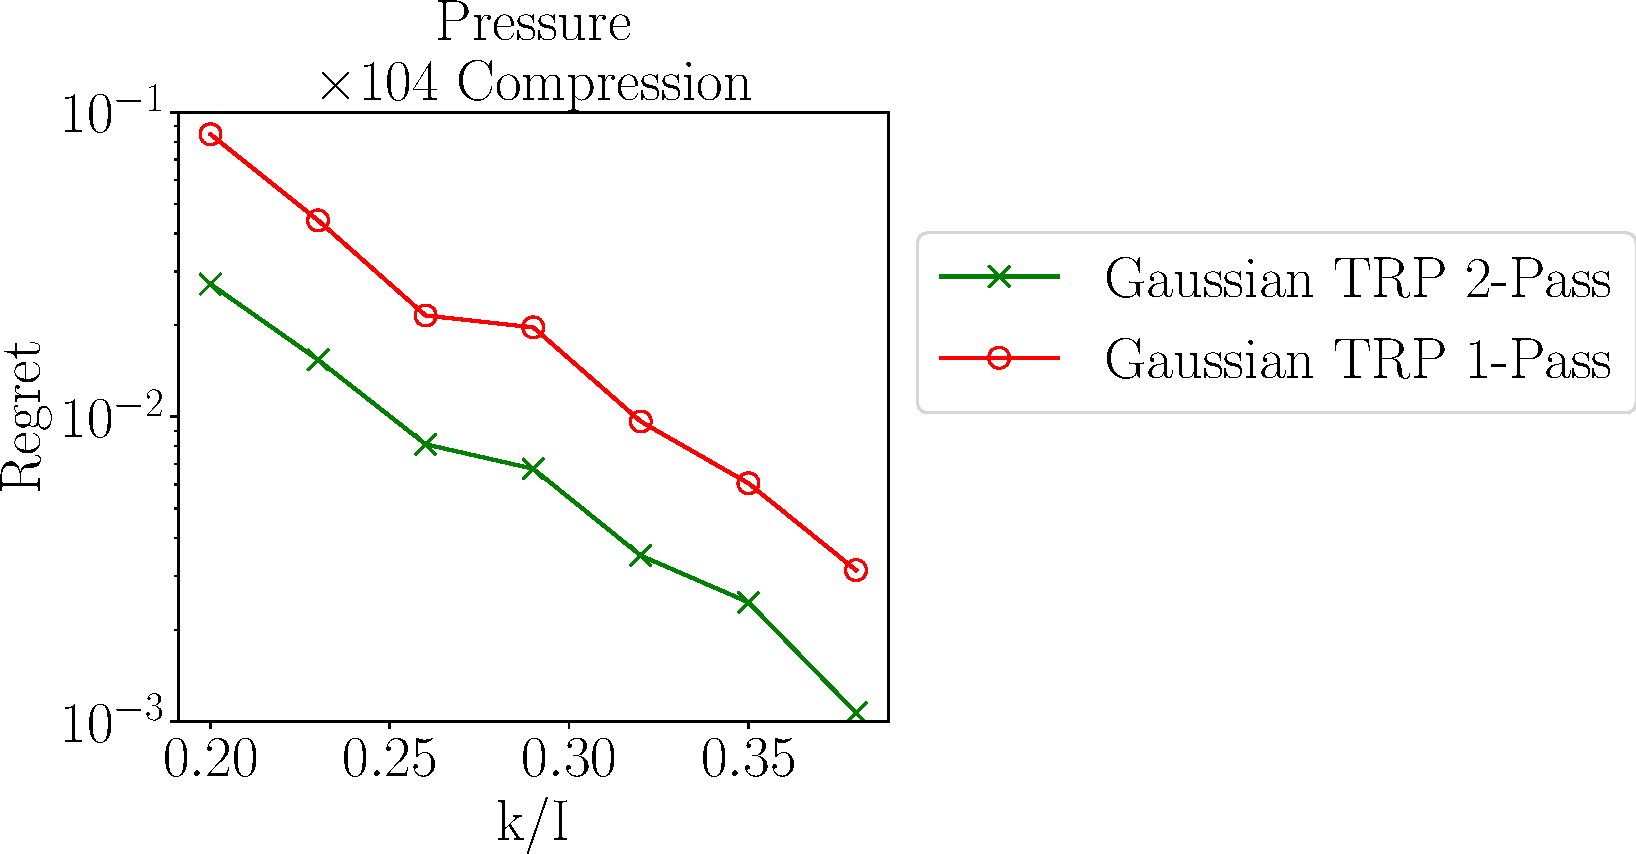
\includegraphics[height=2.9cm]{figure/multi_P_frk10.pdf}\\
	\textbf{Combustion Simulation}\\
	\caption{\textit{Approximations improves with more memory: real data.}
		% The aerosol absorption data	($240 \times 30 \times 192 \times 288$) is from CESM CAM 5.0.
		% The combustion data %for pressure, CO concentration, and temperature
		% (all of size $1408 \times 128 \times 128$)
		% is from \cite{lapointe2015differential}.
		We approximate aerosol absorption and combustion data
		using our one-pass and two-pass algorithms with the Gaussian TRP.
		We compare three target ranks ($r/I = 0.125,0.1,0.067$) for the former,
		and use the same target rank ($r/I = 0.1$) for each measured quantity in
		the combustion dataset.
		Notice $r/I = 0.1$ gives a hundred-fold compression!
	}\label{fig:climate}
\end{figure}

\begin{figure}[h!]
	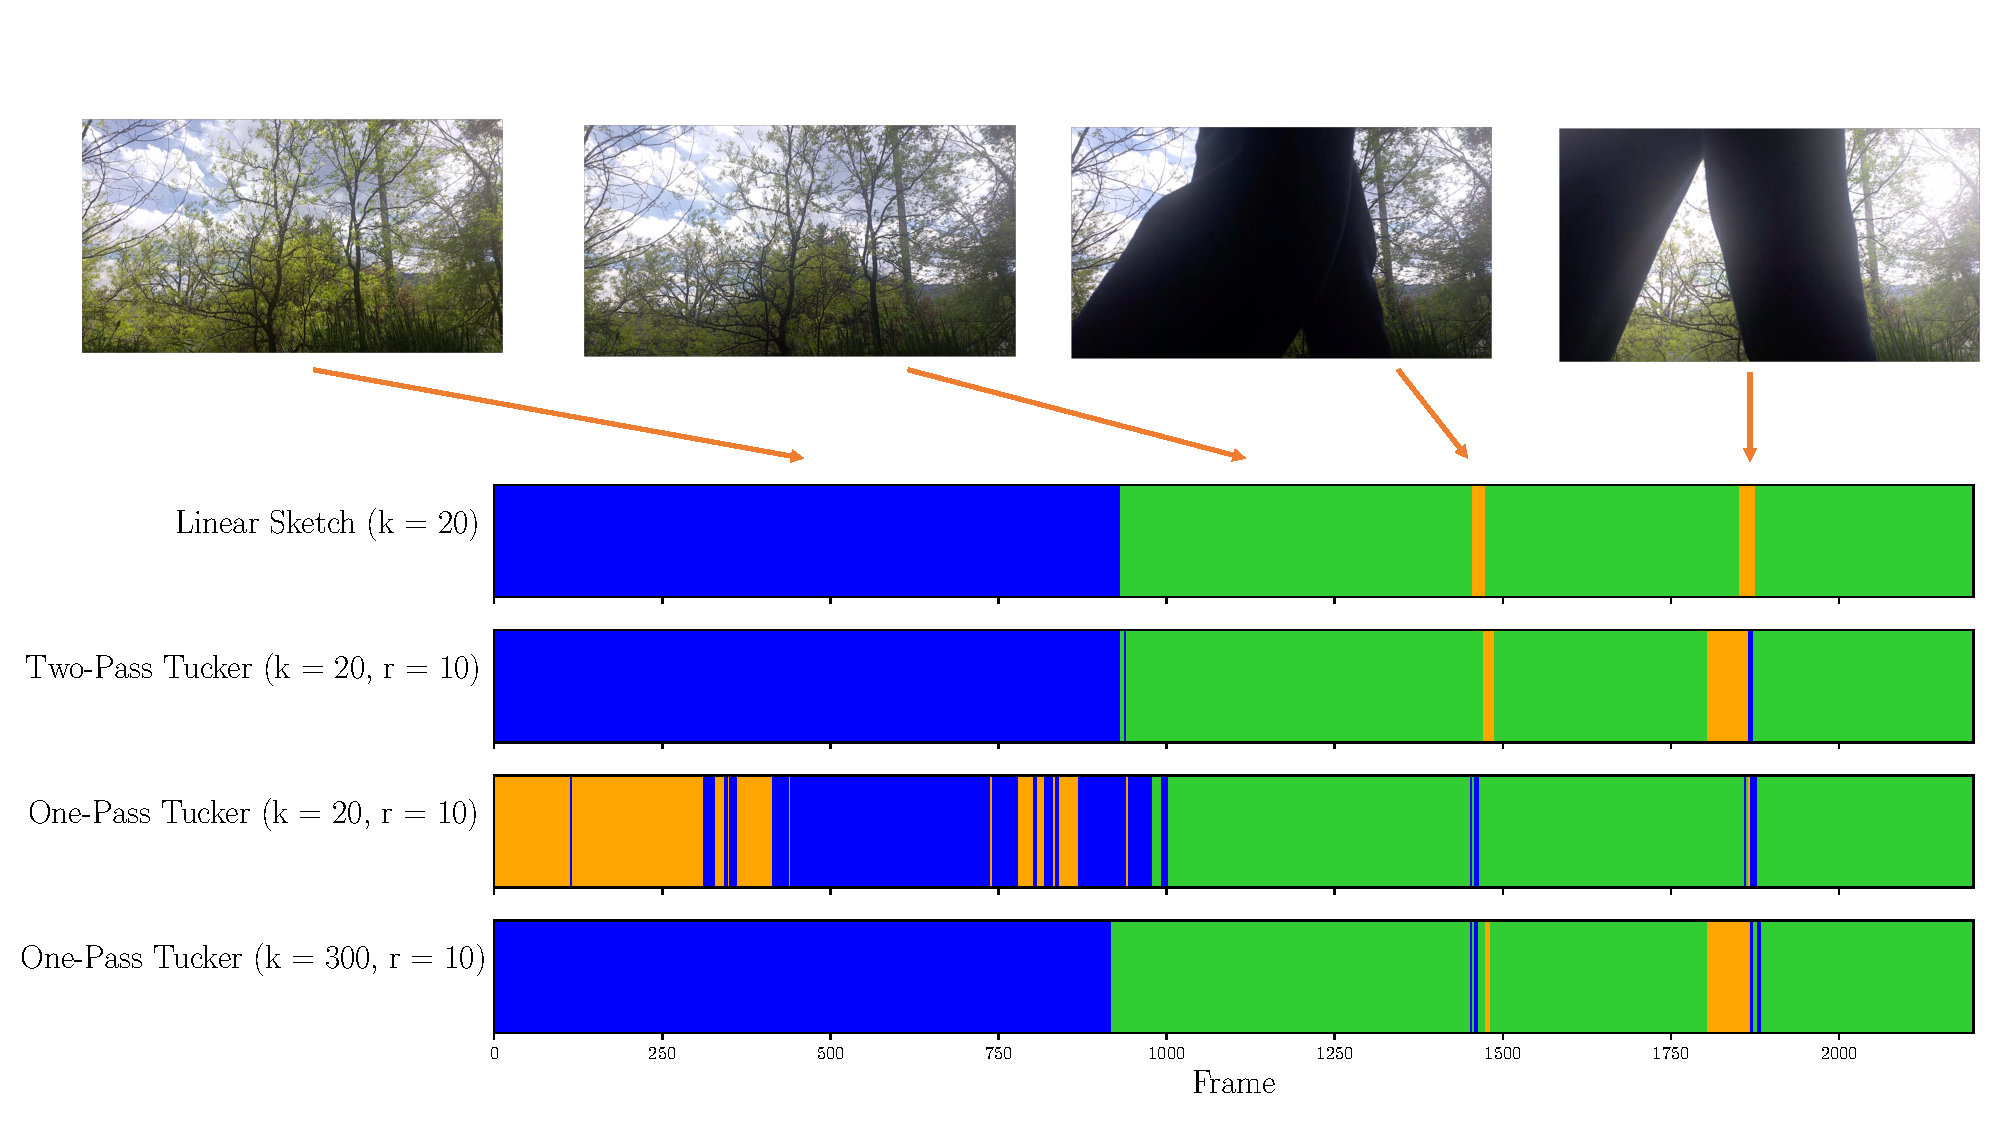
\includegraphics[height=7cm]{figure/video_classification_result.pdf} \\
	\centering
	\textbf{Video Scene Classification}
	\caption{\textit{Video Scene Classification}
		($2200 \times 1080 \times 1980$):
		We classify frames from the video data
		from \cite{malik2018low} (collected as a third order tensor with size $2200 \times 1080 \times 1980$) using $K$-means with $K$=3 on vectors computed using four different methods. $s = 2k+1$ throughout.
		1) The linear sketch along the time dimension (Row 1).
		2-3) the Tucker factor along the time dimension,
		computed via our two-pass (Row 2) and one-pass (Row 3) algorithms.
		%with parameters $r=10$, $k = 20$, and $s = 41$.
		4) The Tucker factor along the time dimension,
		computed via our one-pass (Row 4) algorithm
		%with parameters $r=10$, $k = 300$, and $s = 601$.
		}\label{fig:video}
\end{figure}

\begin{figure}[h!]
	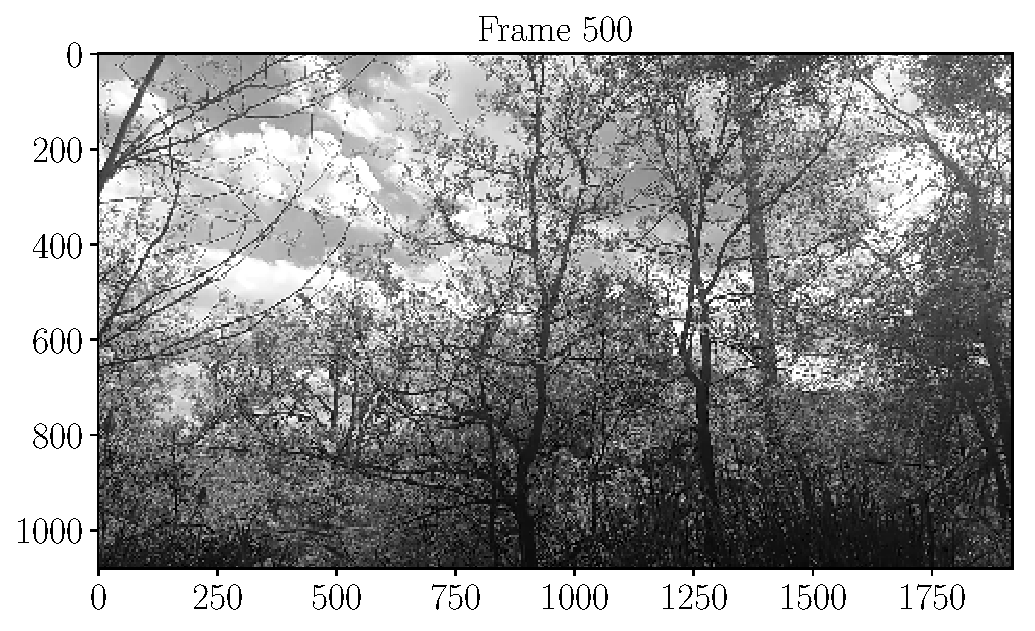
\includegraphics[height=2.4cm]{figure/frame500.pdf}
	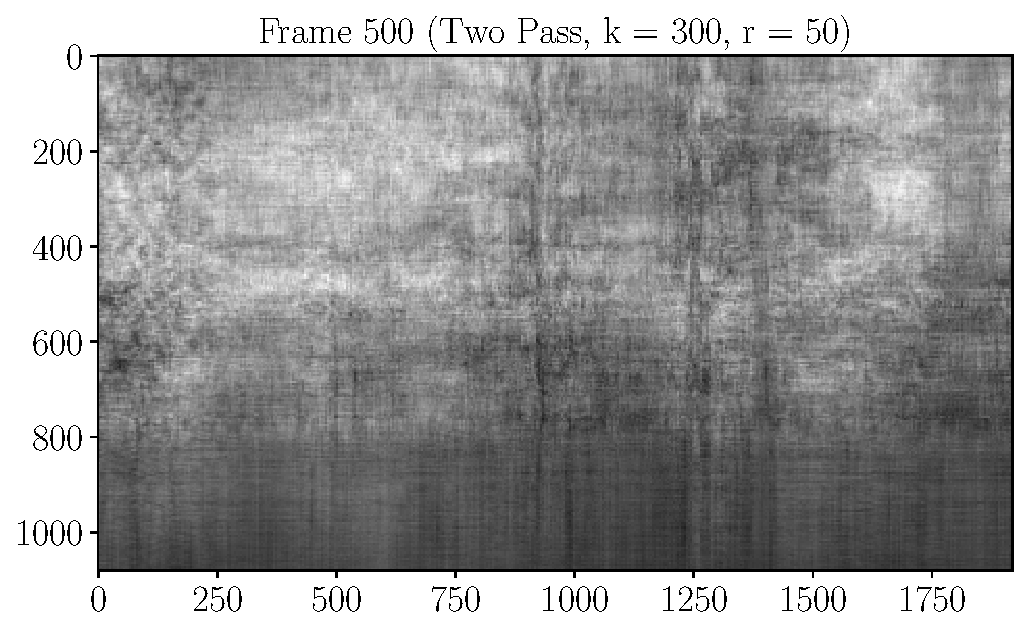
\includegraphics[height=2.4cm]{figure/2pass_k300_r50_frame500.pdf}
	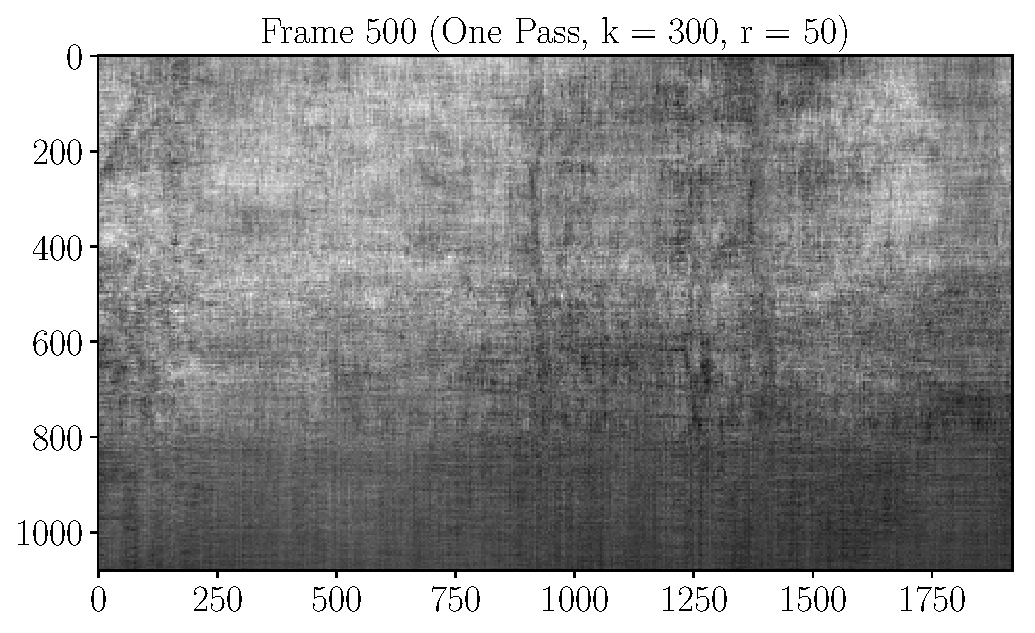
\includegraphics[height=2.4cm]{figure/1pass_k300_r50_frame500.pdf}
	\centering
	\caption{\textit{Visualizing Video Recovery:}
	Original frame (left);
	approximation by two-pass sketch (middle);
	approximation by one-pass sketch (right).
	% Frame 500
	}\label{fig:Frame500}
\end{figure}

\begin{figure}[h!]
	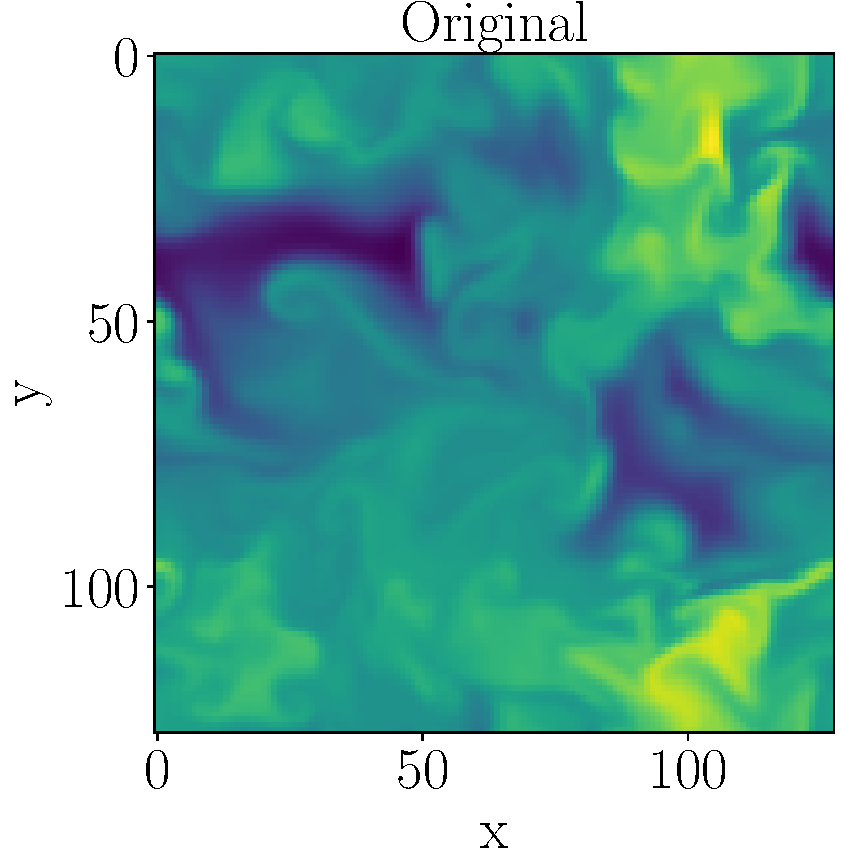
\includegraphics[height=3cm]{figure/T100_original.pdf}
	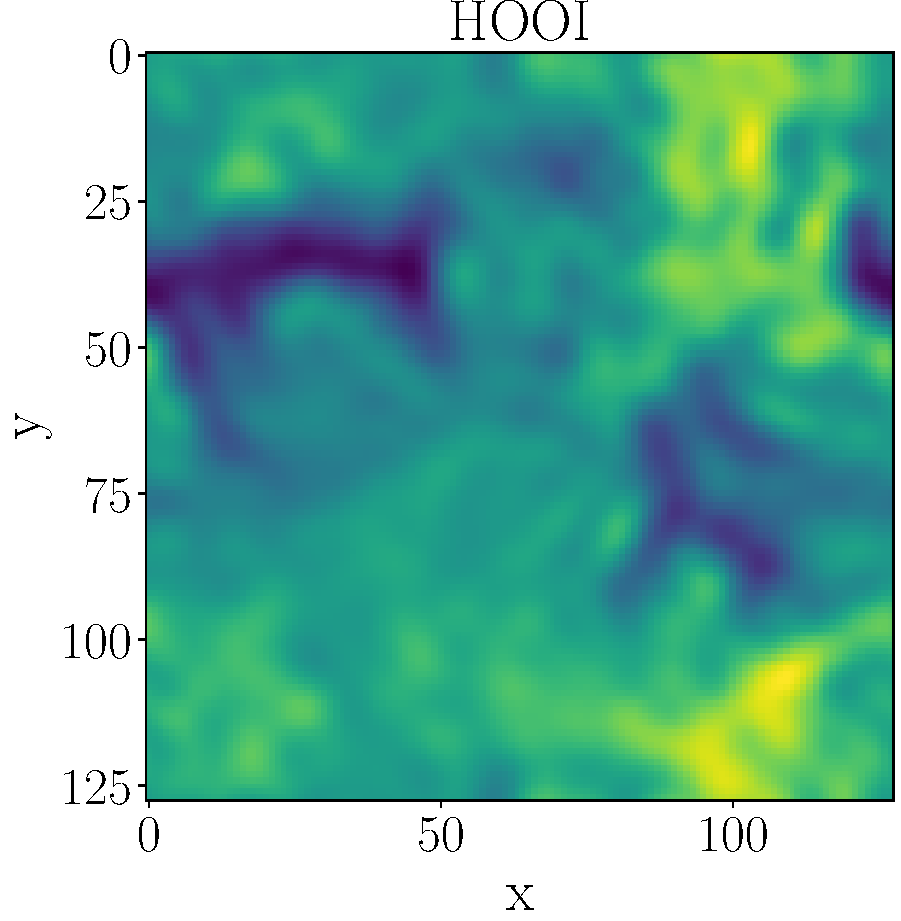
\includegraphics[height=3cm]{figure/T100_hooi.pdf}
	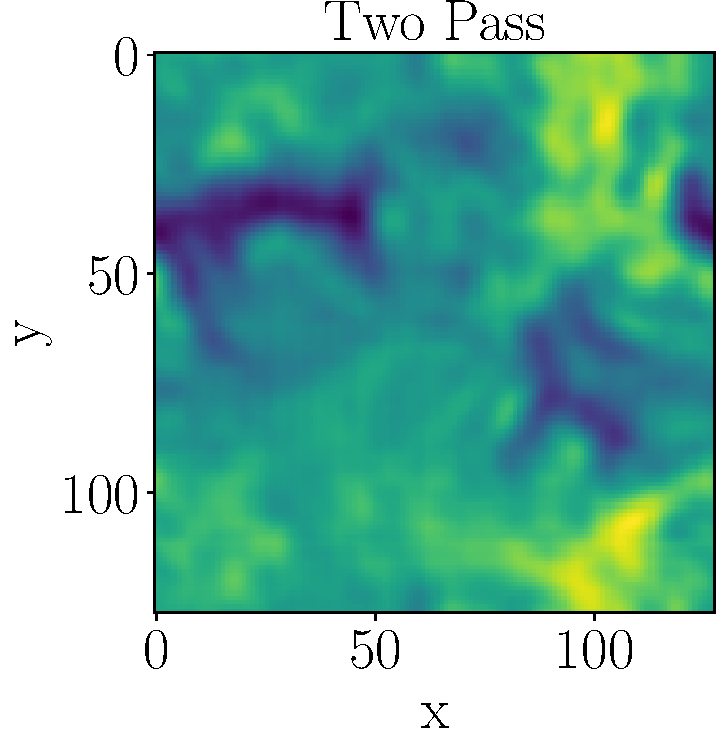
\includegraphics[height=3cm]{figure/T100_2pass.pdf}
	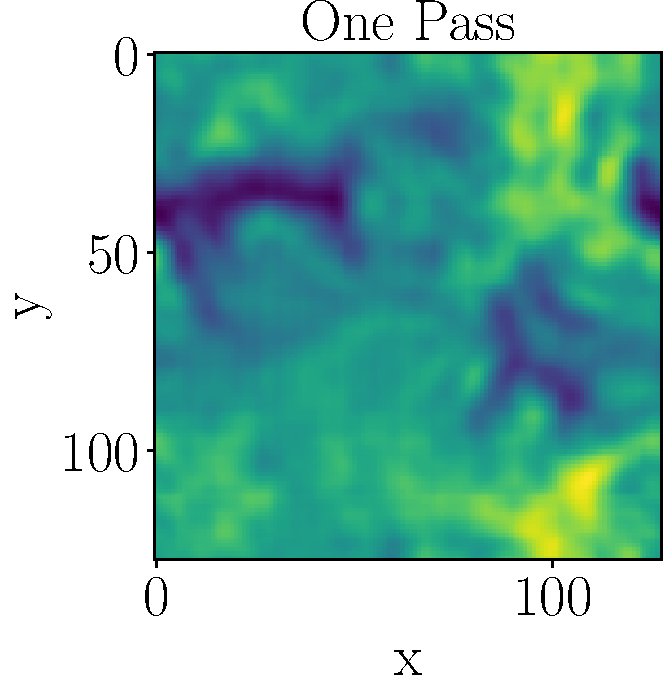
\includegraphics[height=3cm]{figure/T100_1pass.pdf}
	\centering
	\caption{\label{fig:T100}\textit{Visualizing Combustion Simulation:}
	All four figures show a slice of the temperature data along the first dimension.
	The approximation uses
	$\mathbf{r} = (281,25,25)$,
	$\mathbf{k} = (562,50,50)$,
	$\mathbf{s} = (1125, 101, 101)$,
	with the Gaussian TRP in the Tucker sketch.}
\end{figure}

\subsubsection{A second pass reduces error}
The second experiment compares our two-pass and one-pass algorithm.
The design is similar to the first experiment.
\ref{fig:vary-k-600-compare} shows that the two-pass algorithm
typically outperforms the one-pass algorithm,
especially in the high-noise, sparse, or rank-decay case.
Both converge at the same asymptotic rate.
(Results for other input tensors are available
\ifdefined \issupplement
in the supplement.)
\else
%in \ref{fig:vary-k-400-compare-app} and \ref{fig:vary-k-200-compare-app}
in \ref{appendix:more_result}.)
\fi

\subsubsection{Improvement on state-of-the-art}
The third experiment compares the performance of our two-pass and one-pass algorithms
and Tucker TensorSketch (T.--TS), as described in \cite{malik2018low},
the only extant one-pass algorithm.
For a fair comparison, we allocate the same storage budget to each algorithm
and compare the relative error of the resulting fixed-rank approximations.
We approximate synthetic 3D tensors with side length $I = 300$
with Tucker rank $r = 10$.
We use the suggested parameter settings for each algorithm:
$k = 2r$ and $s =2k+1$ for our methods; $K = 10$ for T.--TS.
Our one-pass algorithm
(with the Gaussian TRP)
uses $((2k+1)^N + kIN)$ storage,
whereas T.-TS uses $(Kr^{2N}+Kr^{2N-2})$ storage
\ifdefined \issupplement
(see supplement).
\else
(see \ref{tab:storage-comparison} in \ref{appendix: time-complexity}).
\fi

% Specifically, we choose $k$ linear in log scale within $\in [12,115]$,
% corresponding to $K \in [0.026,12]$ in \cite{malik2018low} \ref{fig:vary-memory}.

Figure \ref{fig:vary-memory} shows that our algorithms generally perform as well as T.--TS,
and dramatically outperforms for small storage budgets.
%two-pass algorithm always outperforms our one-pass algorithm, by a modest margin.
For example, our method achieves 1/50, 1/50, 1/7, and 1/4 the relative error of T.--TS
for low rank and sparse low rank ($\gamma = 0.01$), low rank ($\gamma = 0.1$), and polynomial-decay
input tensors, respectively.
For the low rank ($\gamma = 1$) tensor, the performance of T.--TS is not even monotone as the storage budget increases!
% In the case when the design tensor has a rank decay along its super diagonal, our algorithm is able to easily recover the low-rank signal, while their method is highly unstable and likely to give a worse result even in their suggested setting.
The performance of T.--TS is comparable with that of
the algorithms presented in this paper only when the storage budget is large.
%In both the low-rank and sparse low-rank settings, their method outperforms our method for very large memory usage.

\begin{remark}
	The paper \cite{malik2018low} proposes a multi-pass method, Tucker Tensor-Times-Matrix-TensorSketch (TTMTS) that is dominated by the one-pass method Tucker TensorSketch(TS) in all numerical experiments;
  hence we compare only with T.-TS.
\end{remark}

\subsection{Applications}\label{s-real-data}

We also apply our method to datasets drawn from three application domains:
climate, combustion, and video.
\begin{itemize}
\item \emph{Climate data.}
We consider global climate simulation datasets from
the Community Earth System Model (CESM) Community Atmosphere Model (CAM) 5.0 \cite{hurrell2013community,kay2015community}.
The dataset on aerosol absorption has four dimensions:
times, altitudes, longitudes, and latitudes  ($240 \times 30 \times 192 \times 288$).
% show in appendix
The data on net radiative flux at surface and dust aerosol burden have three dimensions:
times, longitudes, and latitudes ($1200 \times 192 \times 288$).
Each of these quantitives has a strong impact on the absorption of solar radiation and on cloud formation.

\item \emph{Combustion data.}
We consider combustion simulation data from \cite{lapointe2015differential}.
% This paper aims to understand the effect of differential diffusion, distributed burning,
% and local distinction under different circumstances.
The data consists of three measured quantities ---
pressure, CO concentration, and temperature ---
each observed on a $1408 \times 128 \times 128$ spatial grid.
% At each time, we choose three measured quantities out of the 40 measured quantities (all of size $1408 \times 128 \times 128$) at different locations to compress, specifically the pressure, CO concentration, and temperature.

\item \emph{Video data.}
We use our streaming method to cluster frames of a video,
as in \cite{malik2018low}.
Here, a low frame rate camera is mounted in a fixed position as people walk by.
A 3D tensor is constructed with each video frames as a slice.
%The rank of the tensor corresponds to the number of people seen. (The background is rank 2.)
The video consists of 2493 frames, each of size 1080 by 1980.
%  in grayscale,
% thus of size (2493 $\times$ 1080 $\times$ 1980).
As a tensor, stored as a \texttt{numpy.array}, the video data is 41.4 GB in total.
\end{itemize}

\subsubsection{Data compression}
We show that our proposed algorithms are able to
successfully compress climate and combustion data
even when the full data does not fit in memory.
%, we want to compress the huge original tensor into a low-rank Tucker decomposition efficiently.
Since the Tucker rank of the original tensor is unknown, we perform experiments for
three different target ranks. In this experiment, we hope to understand the effect of different choices of storage budget $k$ to
 achieve the same compression ratio. We define the compression ratio
 as the ratio in size between the original input tensor and the output Tucker factors, i.e. $\frac{\prod_{i = 1}^N I_i}{\sum_{i=1}^Nr_iI_i+ \prod_{i = 1}^N r_i}$.
As in our experiments on simulated data, \ref{fig:climate} shows
that the two-pass algorithm outperforms the one-pass algorithm as expected.
However, as the storage budget $k$ increases, both methods converge to the performance of HOOI.
The rate of convergence is faster for smaller target ranks.
Performance of our algorithms on the combustion simulation is qualitatively similar,
but converges faster to the performance of HOOI. \ref{fig:T100} visualizes the recovery of
the temperature data in combustion simulation for a slice along the first dimension. We could observe that the
recovery for both two-pass and one-pass algorithm approximate the recovery from HOOI.
% Indeed, but in general with a faster convergence rate than the climate data even when the data is not perfectly low rank, like the pressure data.
\ifdefined \issupplement
Similar results on other datasets appear in the supplement.)
\else
\ref{fig:srfrad_burden_dust} in \ref{appendix:more_real_data_result}
shows similar results on another dataset.
\fi

\subsubsection{Video scene classification}
We show how to use our single pass method to classify scenes in the video data described above.
The goal is to identify frames in which people appear.
% In our experiment, we split the dataset into nine segments each of size $277 \times 1080 \times 1980$.
% \mnote{why split?}
We remove the first 100 frames and last 193 frames where the camera setup happened,
as in \cite{malik2018low}.
We stream over the tensor and sketch it using parameters $k = 300, s = 601$.
Finally, we compute a fixed-rank approximation with $\mathbf{r} = (10,10,10)$ and $(20,20,20)$.
We apply K-means clustering to the resulting 10 or 20 dimensional vectors
corresponding to each of the remaining 2200 frames.

We experimented with clustering vectors found in three ways:
from the two-pass or one-pass Tucker approximation,
or directly from the factor sketch. % without performing the reconstruction.

When matching the video frames with the classification result,
we can see that the background light is relatively dark at the beginning,
thus classified into \texttt{Class} $0$.
After a change in the backgroun light,
most other frames of the video are classified into \texttt{Class} $1$.
When a person passes by the camera, the frames are classified into \texttt{Class} $2$.
Right after the person passed by, the frames are classified into \texttt{Class} $0$,
the brighter background scene, due to the light adjustment.

Our classification results (using the linear sketch or approximation)
are similar to those in \cite{malik2018low}
while using only $1/500$ as much storage; the one pass approximation
requires more storage (but still less than \cite{malik2018low}) 
to achieve similar performance.
In particular, using the sketch itself, rather than the Tucker approximation,
to summarize the data enables very efficient video scene classification.

On the other hand, to reconstruct the original video frames
we require much larger $\mathbf{k}$ and $\mathbf{r}$:
the video is not very low rank along the spatial dimensions.
\ref{fig:Frame500} shows that
even with $\mathbf{s} = {601, 601, 601}, \mathbf{k} = (300, 300, 300), \mathbf{r} = (50, 50, 50)$, the recovered frame is very noisy.
% The memory and computational requirements of HOOI exceed our capacity,
% so we cannot apply it to the video data.

\section{Conclusion}
This paper proposes a practical one-pass algorithm to compute the
Tucker decomposition of a tensor with provable guarantees.
Our algorithm uses a dimension reduction map to summarize the data in a linear sketch.
This sketch can be efficiently stored or transmitted, which enables applications in modern large-scale setting, including streaming and distributed data storage, or computational environment with limited memory.
We give the first comprehensive error analysis for one-pass Tucker decomposition algorithm in \ref{thm:low_rank_err}
and \ref{thm:fix_rank_err} for the tensor
approximation with error growing only linearly with the order $N$ of the tensor. In practice, our algorithm significantly outperforms the current state-of-the-art one-pass Tucker decomposition algorithm \cite{malik2018low} in the limited memory setting and noisy setting with much greater stability. Also, our one-pass achieves the same performance in \cite{malik2018low}'s suggested setting when the memory requirement is much higher than our suggested setting.
Our algorithm is available as an open-source python package.
% no acknowledgements in anonymous submission
% \subsubsection*{Acknowledgements}
% The authors would like to thank Guillaume Blanquart for discussing the applications of our sketching algorithm in combustion simulation data. The research is sponsored by ...

%\clearpage

\clearpage
\begin{subappendices}
\section{Proof of Main Results}
\label{appendix:proof-main-result}
% To bound the approximation error of the algorithms presented in the main body
% of this paper, we first develop several structural results showing
% an additive decomposition of the error.
% First, the total error is the sum of the error due to sketching
% and the error due to fixed rank approximation.
% Second, the sketching error is the sum of the error due to the factor matrix
% approximations and to the core approximation.
% Third, the error due to the factor matrix approximations
% is the sum of the error in each the modes,
% as the errors due to each mode are mutually orthogonal.
% This finishes the approximation error bound for the two pass algorithm, \ref{thm:low_rank_err_two_pass}.
% As for the error due to the core approximation,
% we give a combinatorial argument to rewrite the approximation error in the core tensor
% as a sum over each mode of errors that are mutually orthogonal.
% Indeed, these errors have the same form as the errors due to the factor matrix approximations,
% scaled down by a factor $\Delta(k,s)$ that depends on the sketch sizes $\V{k}$ and $\V{s}$.
% This argument shows the error due to the core approximation
% is at most a factor $\Delta(k,s)$ times the error due to the factor matrix approximation.

% Yiming wrote:
% For low rank approximation, since there is no any optimization procedure involved, all the errors come from sketching stage. For fixed rank approximation, we also need to take the recovery error (from Tucker decomposition)  into consideration. But for tensor decomposition, the approximation error is impossible to be described as clear as that in matrix case(singular value decomposition). we include the best approximation error in our result. Essentially for both case, our theory focuses in building statistical  error bound introduced by the sketching and leave the recovery error in terms of the best approximation error: $\|\T{X} - \llbracket \T{X} \rrbracket_\mathbf{r}\|_F$.
%
% For sketching stage, we consider errors introduced by arm sketch and core sketch
% respectively. Arm sketch essentially is a series of projection of original tensor to column space the sketch corresponding along each mode. We demonstrate that we can decompose the error as sum of errors along each mode by showing they are orthogonal to each other. For the error from core sketch, by some combinatoric argument, we essentially treat the approximation error for core tensor as $\sum_n \rm{Approx}(\T{Z}_n)$ where $\sum_n \T{Z}_n = \T{X} - \T{\hat{X}}$, $\langle \T{Z}_m, \T{Z}_n \rangle = 0$ and $\rm{Approx}(\T{Z}_n)$ is some approximation of $\T{Z}_n$ satisfying $\|\rm{Approx}(\T{Z}_n) -\T{Z}_n\|_F \le \Delta(k,s) \|\T{Z}_n\|_F$ where $\Delta(k,s)$ is a constant depending in sketch size $k,s$. This essentially claims that the error from core sketch is at most $\Delta(k,s)$ of error from arm sketch.

\subsection{Error bound for the two pass approximation Algorithm \ref{alg:two_pass_low_rank_appro}}
\begin{proof}[Proof of Theorem \ref{thm:low_rank_err_two_pass}]
Suppose $\T{\hat{X}}_2$ is the low-rank approximation from \ref{alg:two_pass_low_rank_appro}.
Use the definition of the mode-$n$ product to see
\begin{equation*}
\begin{aligned}
\T{\hat{X}}_2 &=  \left[\T{X}\times_1 \mathbf{Q}_1^\top \times_2 \cdots \times_N \mathbf{Q}_N^\top\right] \times_1 \mathbf{Q}_1\times_1 \cdots\times_N \mathbf{Q}_N\\
&= \T{X}\times_1 \mathbf{Q}_1\mathbf{Q}_1^\top \times_2 \cdots \times_N \mathbf{Q}_N\mathbf{Q}_N^\top.
\end{aligned}
\end{equation*}
Although it seems that we sequentially project tensor $\T{X}$ to column space spanned with $\mathbf{Q}_n$, but since mode product is exchangeable, in fact $\hat{\T{X}}_2$ is the projection to space $\{ \T{X} : \T{X}^{(n)} 
\in \mathbf{col}(\mathbf{Q}_n) \}$.  This is a generalization of projection matrix where \cite{de2008tensor} has a very detailed  explanation and it is referred as multi-linear orthogonal projection.  Following exact techniques in Theorem 5.1 in \cite{vannieuwenhoven2012new} by sequentially applying Pythagorean theory sequentially we can show that 
\begin{equation}
\|\hat{\T{X}}_2 - \T{X}\|_F^2 \le \sum_{n=1}^N  \left \| (\mathbf{I} - \mathbf{Q}_n\mathbf{Q}_n^\top) \mathbf{X}^{(n)} \right\|_F^2 .
\end{equation}
Then taking expectation on $\mathbf{Q}_n$, and applying Lemma \ref{lemma:sketchy_column_space_err} we complete the proof. 




\end{proof}

\subsection{Error bound for the one pass approximation Algorithm \ref{alg:one_pass_low_rank_appro}}
\begin{proof}[Proof of Theorem \ref{thm:low_rank_err}]
We show the approximation error can be decomposed as
the error due to the factor matrix approximations
and the error due to the core approximation.
Let $\T{\hat{X}}_1$ be the one pass approximation from \ref{alg:one_pass_low_rank_appro}, and let
\begin{equation}
\T{\hat{X}}_2 = \T{X}\times_1 \mathbf{Q}_1\mathbf{Q}_1^\top \times_2 \cdots \times_N \mathbf{Q}_N\mathbf{Q}_N^\top,
\end{equation}
be the two pass approximation from \ref{alg:two_pass_low_rank_appro}.
The difference in one-pass and two-pass approximation is in the 
core: 
\begin{equation}
\begin{aligned}
\T{\hat{X}}_1-\hat{\T{X}}_2= (\T{W}-\T{X}\times_1 \mathbf{Q}_1^\top \times_2 \cdots \times_N \mathbf{Q}_n^\top)  \times_1 \mathbf{Q}_1 \dots \times_N \mathbf{Q}_N. \nonumber
\end{aligned}
\end{equation}
Thus $\T{\hat{X}}_1-\hat{\T{X}}_2$ is in the space defined above:  $\{ \T{X} : \T{X}^{(n)} 
\in \mathbf{col}(\mathbf{Q}_n) \}$ while as pointed before $\hat{\T{X}}_2 - \T{X}$ is perpendicular  to that space.  Therefore, 

\begin{equation}
\label{eq:inner_zero}
\langle \hat{\T{X}}_1 - \hat{\T{X}}_2, \hat{\T{X}}_2 - \T{X} \rangle = 0.
\end{equation}


Now we use the (expectation of) the Pythagorean theorem 
to bound the expected error of the one pass approximation:
\begin{equation}
\label{eq:error_decom}
 \mathbb{E}\| \hat{\T{X}}_1- \T{X} \|_F^2 = \mathbb{E}\| \hat{\T{X}}_1 - \hat{\T{X}}_2\|_F^2 + \mathbb{E} \|\hat{\T{X}}_2 - \T{X} \|_F^2.
\end{equation}



Consider the first term which is due to core approximation. Based in the definition of $\hat{\T{X}}_1$ and $\tilde{\T{X}}_2$ we can see that 
\begin{align*}
\|\hat{\T{X}}_1 - \hat{\T{X}}_2\|^2_F &=
\|(\T{W}_1 - \T{X}\times_1 \mathbf{Q}_1^\top \cdots \times_N \mathbf{Q}^\top_N)\times_1 \mathbf{Q}_1\cdots \times_N \mathbf{Q}_N \|^2_F\\
& = \|(\T{W}_1- \T{X}\times_1 \mathbf{Q}_1^\top \cdots \times_N \mathbf{Q}^\top_N)\|_F^2,
\end{align*}
where we use the invariance of the Frobenius norm under orthonormal transformations to get the second line.
Now using \ref{lemma:err_core_sketch} to bound for the error due to the core approximation as
%(the first term in \eqref{eq:error_decom}) as
\begin{equation}
\mathbb{E} \|\hat{\T{X}}_1- \hat{\T{X}}_2\|^2_F \le \Delta \left[ \sum_{n=1}^N \left(1+\frac{\rho_n}{k_n-\rho_n-1}\right)(\tau^{(n)}_{\rho_n})^2\right].\nonumber
\end{equation}

Finally, as shown in proof for  \ref{thm:low_rank_err_two_pass} to
bound the error due to the factor matrix approximations
(the second term in \eqref{eq:error_decom}) as
\begin{equation}
\mathbb{E}\|\hat{\T{X}}_2 - \T{X} \|_F^2 \le \left[ \sum_{n=1}^N \left(1+\frac{\rho_n}{k_n-\rho_n-1}\right)(\tau^{(n)}_{\rho_n})^2\right].\nonumber
\end{equation}
Summing these two bounds finishes the proof.
\end{proof}

\subsection{Error bound for the fixed rank approximation Algorithm  \ref{alg:one_pass_fix_rank_appro}}

\begin{proof}[Proof of Theorem \ref{thm:fix_rank_err}]
Our argument follows the proof of \cite[Proposition 6.1]{tropp2017practical}:
\begin{equation}
\begin{aligned}
&\|\T{X} - \llbracket \hat{\T{X}} \rrbracket_\mathbf{r}\|_F \le \|\T{X} -  \hat{\T{X}}\|_F+\|\hat{\T{X}} -  \llbracket\hat{\T{X}}\rrbracket_\mathbf{r}\|_F\\
&\le \|\T{X} -  \hat{\T{X}}\|_F+\|\hat{\T{X}} -  \llbracket \T{X}\rrbracket_\mathbf{r}\|_F \\
& \le \|\T{X} -  \hat{\T{X}}\|_F+\|\hat{\T{X}} - \T{X}  + \T{X} - \llbracket \T{X}\rrbracket_\mathbf{r}\|_F \\
&\le 2\|\T{X} - \hat{\T{X}} \|_F + \|\T{X} -  \llbracket \T{X} \rrbracket_\mathbf{r}\|_F.\nonumber
\end{aligned}
\end{equation}
The first and the third line are the triangle inequality,
and the second line follows from the definition of the best rank-$r$ approximation.
Take the expectation of $\|\T{X} - \hat{\T{X}} \|_F$ and
use Jensen's inequality $\mathbb{E}\|\T{X} - \hat{\T{X}} \|_F \le \sqrt{\mathbb{E} \|\T{X} - \hat{\T{X}} \|_F^2}$
to finish the proof.
\end{proof}

\section{Probabilistic Analysis of Core Sketch Error}
This section contains the most technical part of our proof.
We provide a probabilistic error bound for the difference between the
two pass core approximation $\T{W}_2$
from Algorithm \ref{alg:two_pass_low_rank_appro}
and the one pass core approximation $\T{W}_1$
from Algorithm \ref{alg:one_pass_low_rank_appro}.
% We first prove that this error
% will show how to decompose this error first, and
% then take the expectation to obtain the probabilistic error bound.

Introduce for each $n\in[N]$ the orthonormal matrix $\M{Q}_n^\bot$ that forms
a basis for the subspace orthogonal to $\M{Q}_n$, so that
$\M{Q}_n^\bot (\M{Q}_n^\bot)^\top = \M{I} - \M{Q}_n\M{Q}_n^\top$.
Next, define
\begin{equation}
\label{eq: def-proj-Q}
\begin{aligned}
\M{\Phi}_n^Q = \M{\Phi}^\top_n \M{Q}_n  ,~~~~\M{\Phi}_n^{Q^\bot} = \M{\Phi}^\top_n \M{Q}_n^\bot.
\end{aligned}
\end{equation}
Recall that the DRMs $\M{\Phi}_n$ are i.i.d. Gaussian. Hence conditional on $\M{Q}_n$,
$\M{\Phi}_n^Q$ and $\M{\Phi}_n^{Q^\bot}$ are independent.

\subsection{Decomposition of Core Approximation Error}
In this section, we characterize the
difference between the one and two pass core approximations
$\T{W}_1-\T{W}_2 = \T{W}_1 - \T{X}\times_1 \M{Q}_1^\top \dots \times_N \M{Q}_N^\top$.
\begin{lem}
\label{lemma:core_error_decomposition}
Suppose that $\M{\Phi}_n$ has full column rank for each $n \in [N]$.
Then
\begin{equation}
\T{W}_1-\T{W}_2 = \T{W}_1 - \T{X}\times_1 \M{Q}_1^\top \dots \times_N \M{Q}_N^\top =
\sum_{(i_1,\dots, i_N) \in \{0,1\}^N, \sum_{j=1}^N i_j \geq 1} \T{Y}_{i_1\dots i_N}, \nonumber
\end{equation}
where
\begin{equation}
\label{eq:def_each_part}
\begin{aligned}
\T{Y}_{i_1\dots i_N} &= \T{X}\times_1 \left(\mathbf{1}_{i_1=0}\M{Q}_1^\top + \mathbf{1}_{i_1=1}(\M{\Phi}_1^{Q_1})^\dag  \M{\Phi}_1^{Q_1^\bot}(\M{Q}_1^\bot)^\top \right)\\
&\times_2 \cdots \times_N \left(\mathbf{1}_{i_N=0}\M{Q}_N^\top + \mathbf{1}_{i_1=1}(\M{\Phi}_N^{Q_N})^\dag  \M{\Phi}_N^{Q_N^\bot}(\M{Q}_N^\bot)^\top \right).
\end{aligned}
\end{equation}
\end{lem}
\begin{proof}
Let $\T{H}$ be the core sketch from \ref{alg:tensor_sketch}.
Write %the one pass core approximation
$\T{W}_1$ as
\begin{equation}
\begin{aligned}
\T{W}_1 &= \T{H}\times_1 (\M{\Phi}_1^\top \M{Q}_1)^\dag \times_2 \cdots \times_N (\M{\Phi}^\top_N \M{Q}_N)^\dag \\
&= (\T{X} -  \hat{\T{X}}_2)\times_1 \M{\Phi}^\top_1 \times_2 \cdots \times_N \M{\Phi}^\top_N  \times_1 (\M{\Phi}^\top_1 \M{Q}_1)^\dag \times_2 \cdots \times_N (\M{\Phi}^\top_N \M{Q}_N)^\dag
\\
&+ \hat{\T{X}}_2\times_1 \M{\Phi}^\top_1 \times_2 \cdots \times_N \M{\Phi}^\top_N \times_1 (\M{\Phi}^\top_1 \M{Q}_1)^\dag \times_2 \cdots \times_N (\M{\Phi}^\top_N \M{Q}_N)^\dag.\nonumber
\end{aligned}
\end{equation}
Using the fact that $(\M{\Phi}^\top_n \M{Q}_n)^\dag (\M{\Phi}^\top_n \M{Q}_n) =\M{I}$, we can simplify the second term as
\begin{equation}
\begin{aligned}
&\tilde{\T{X}}\times_1 \M{\Phi}^\top_1 \times_2 \cdots \times_N \M{\Phi}^\top_N \times_1 (\M{\Phi}^\top_1 \M{Q}_1)^\dag \times_2 \cdots \times_N (\M{\Phi}^\top_N \M{Q}_N)^\dag   \\
& = \T{X}\times_1 (\M{\Phi}^\top_1 \M{Q}_1)^\dag \M{\Phi}^\top_1\M{Q}_1\M{Q}_1^\top \times_2 \cdots \times_N (\M{\Phi}_N^\top \M{Q}_N)^\dag \M{\Phi}_N^\top\M{Q}_N\M{Q}_N^\top\\
& = \T{X}\times_1 \M{Q}_1^\top \times_2 \cdots \times_N \M{Q}_N^\top, \nonumber
\end{aligned}
\end{equation}
which is exactly the two pass core approximation $\T{W}_2$.
Therefore
\begin{equation}
\begin{aligned}
&\T{W}_1 -\T{W}_2= (\T{X} -  \tilde{\T{X}})\times_1 \M{\Phi}^\top_1 \times_2 \cdots \times_N \M{\Phi}^\top_N  \times_1 (\M{\Phi}^\top_1 \M{Q}_1)^\dag \times_2 \cdots \times_N (\M{\Phi}^\top_N \M{Q}_N)^\dag. \nonumber
\end{aligned}
\end{equation}
We continue to simplify this difference:
\begin{equation}
\begin{aligned}
(\T{X} -  \tilde{\T{X}})&\times_1 \M{\Phi}^\top_1 \times_2 \cdots \times_N \M{\Phi}^\top_N  \times_1 (\M{\Phi}^\top_1 \M{Q}_1)^\dag \times_2\cdots \times_N (\M{\Phi}^\top_N \M{Q}_N)^\dag \label{eq:core_err_decom} \\
& =(\T{X} -  \tilde{\T{X}})\times_1 (\M{\Phi}^\top_1\M{Q}_1)^\dag \M{\Phi}^\top_1 \times_2\cdots \times_N (\M{\Phi}^\top_N\M{Q}_N)^\dag \M{\Phi}_N^\top \\
& =  (\T{X} -  \tilde{\T{X}}) \times_1 (\M{\Phi}^\top_1\M{Q}_1)^\dag \M{\Phi}^\top_1(\M{Q}_1\M{Q}_1^\top + \M{Q}_1^\bot (\M{Q}_1^\bot)^\top)\dots  \\
& \times_N (\M{\Phi}^\top_N\M{Q}_N)^\dag \M{\Phi}^\top_N(\M{Q}_N\M{Q}_N^\top + \M{Q}_N^\bot (\M{Q}_N^\bot)^\top)\\
& = (\T{X} -  \tilde{\T{X}}) \times_1 (\M{Q}_1^\top + (\M{\Phi}_1^Q)^\dag  \M{\Phi}_1^{Q^\bot}(\M{Q}_1^\bot)^\top)\times_2\dots \\
 &\times_N (\M{Q}_N^\top + (\M{\Phi}_N^{Q_N})^\dag  \M{\Phi}_N^{Q_N^\bot}(\M{Q}_N^\bot)^\top).
\end{aligned}
\end{equation}
Many terms in this sum are zero. We use the following two facts:
\begin{enumerate}
\item $(\T{X} - \tilde{\T{X}})\times_1 \M{Q}_1^\top\dots \times_N \M{Q}_N^\top = 0$.
\item For each $n \in [N]$, $\tilde{\T{X}}\times_n (\M{\Phi}_n^{Q_n})^\dag  \M{\Phi}_n^{Q_n^\bot}(\M{Q}_n^\bot)^\top =  0$.
\end{enumerate}
Here $0$ means a tensor with all zero elements.
These facts can be obtained from the exchange rule of the mode product and the orthogonality between $\M{Q}_n^\bot$ and $\M{Q}_n$.
 %$\M{Q}_n^\top (\M{I} - \M{Q}_n \M{Q}_n^\top) = 0$; $(\M{Q}_n^\bot)^\top \M{Q}_n = 0$.
Using these two facts, we find that only the terms $\T{Y}_{i_1\dots i_N}$ (defined in \eqref{eq:def_each_part})
remain in the expression.
Therefore, to complete the proof, we write \eqref{eq:core_err_decom} as
\begin{equation}
\sum_{(i_1,\dots, i_N) \in \{0,1\}^N, \sum{n=1}^N i_n\neq 0} \T{Y}_{i_1\dots i_N}.\nonumber
\end{equation}
\end{proof}

\subsection{Probabilistic Core Error Bound}
In this section, we derive a probabilistic error bound
based on the core error decomposition from  Lemma \ref{lemma:core_error_decomposition}.
\begin{lem}
\label{lemma:err_core_sketch}
Sketch the tensor $\T{X}$ using a Tucker sketch with parameters $\V{k}$ and $\V{s} > 2 \V{k}$
with i.i.d. Gaussian $\mathcal N(0,1)$ DRMs.
Define $\Delta = \max_{n=1}^N \frac{k_n}{s_n-k_n-1}$.
Then for any natural numbers $1 \le \V{\rho} < \V{k}-1$,
\begin{equation}
\mathbb{E} \|\T{W}_1 - \T{X}\times_1 \M{Q}_1^\top \dots \times_N \M{Q}_N^\top\|_F^2 \le \Delta \left[ \sum_{n=1}^N \left(1+\frac{\rho_n}{k_n-\rho_n-1}\right)(\tau^{(n)}_{\rho_n})^2\right]. \nonumber
\end{equation}
\end{lem}
\begin{proof}
It suffices to show
\begin{equation}\label{eq:factor-matrix-error-bounds-core-error}
\mathbb{E}\left[ \|\T{W}_1 - \T{X}\times_1 \M{Q}_1^\top \dots \times_N \M{Q}_N^\top\|_F^2 \mid \M{\Omega}_1, \cdots, \M{\Omega}_N \right] \le \Delta  \|\T{X} - \hat{\T{X}}_2\|_F^2.
\end{equation}
Then take the expectation with respect to $\M{\Omega}_1, \cdots,  \M{\Omega}_N$
and apply results in \ref{thm:low_rank_err_two_pass} to bound $\|\T{X} - \hat{\T{X}}_2\|_F^2$ to finish the proof.
To show \ref{eq:factor-matrix-error-bounds-core-error},
we will use the fact that the core DRMs $\{\M{\Omega_n}\}_{n \in [N]}$
are independent of the factor matrix DRMs $\{\M{\Phi_n}\}_{n \in [N]}$,
and that the randomness in
each factor matrix approximation $\M{Q}_n$
comes solely from $\M{\Omega}_n$.
% each factor matrix approximation $\M{Q}_n$
% comes solely from the factor matrix DRM $\M{\Omega}_n$.

For $i\in \{0,1\}^N$, define $\T{B}_{i_1\dots i_N} =$
\[
\T{X}\times_1 (\mathbf{1}_{i_1=0}\M{Q}_1\M{Q}_1^\top + \mathbf{1}_{i_1=1}\M{Q}_1^\bot(\M{Q}_1^\bot)^\top)\cdots\times_N(\mathbf{1}_{i_N=0}\M{Q}_N\M{Q}_N^\top + \mathbf{1}_{i_N=1}\M{Q}_N^\bot(\M{Q}_N^\bot)^\top).
\]
\ref{lemma:core_error_decomposition} decomposes the core error as the sum of
$\T{Y}_{i_1\cdots i_n}$ where $\sum_{n=1}^N i_n \geq 1$.
Applying \ref{lemma:expectation_inverse_gaussian} and using 
the orthogonal invariance of the Frobenius norm,  we observe
\begin{equation}
\mathbb{E} \left[ \|\T{Y}_{i_1\dots i_N}\|_F^2 \mid \M{\Omega}_1 \cdots \M{\Omega}_N \right] =\left(\prod_{n=1}^N \Delta_n^{i_n}\right)
\|\T{B}_{i_1\dots i_N}\|_F^2 \le \Delta \|\T{B}_{i_1\dots i_N}\|_F^2\nonumber
\end{equation}
when $\sum_{n=1}^N i_n \geq 1$,
where $\Delta_n = \frac{k_n}{s_n-k_n-1}<1$ and $\Delta = \max_{n=1}^N \Delta_n$.

Suppose $\mathbf{q}_1, \mathbf{q}_2 \in \{0,1\}^N$ are  index (binary) vectors of length $N$.
For different indices $\mathbf{q}_1$ and $\mathbf{q}_2$, there exists some $1\le r\le N$
such that their $r$-th element is different.
Without loss of generality, assume $\mathbf{q}_1(r) = 0$ and $\mathbf{q}_2(r)=1$ to see
\begin{equation}\label{eq:inner_prod2}
\langle \T{B}_{q_1}, \T{B}_{q_2}\rangle = \langle \dots \M{Q}_r^\top \M{Q}_r^\bot \dots\rangle  = 0.
\end{equation}
Similarly we can show that the inner product between $\T{Y}_{q_1}$ and $\T{Y}_{q_2}$ is zero with different $\mathbf{q}_1, \mathbf{q}_2$.  Noticing that  $\T{B}_{0,\ldots, 0} = \hat{\T{X}}_2$, we have
\begin{align*}
\|\T{X} - \hat{\T{X}}_2\|_F^2
&= \left\|\sum_{(i_1,\dots, i_N) \in \{0,1\}^N, \sum_{n=1}^N i_n \geq 1}  \T{B}_{i_1\dots i_N}\right \|_F^2
&= \sum_{\substack{(i_1,\dots, i_N) \in \{0,1\}^N, \\ \sum_{n=1}^N i_n \geq 1}} \|\T{B}_{i_1\dots i_N}\|_F^2.
\end{align*}
Putting all these together and using the Pythagorean theorem,
to show \ref{eq:factor-matrix-error-bounds-core-error}:
\begin{equation}
\begin{aligned}
&\mathbb{E}\left[ \|\T{W} - \T{X}\times_1 \M{Q}_1^\top \dots \times_N \M{Q}_N^\top\|_F^2 \mid \M{\Omega}_1, \cdots, \M{\Omega}_N \right] \\
& = \sum_{(i_1,\dots, i_N) \in \{0,1\}^N, \sum_{n=1}^N i_n \geq 1} \mathbb{E} \left[\|\T{Y}_{i_1\dots i_N}\|_F^2 \mid \M{\Omega_1}, \dots, \M{\Omega}_N\right]\\
&\le \Delta \left(\sum_{(i_1,\dots, i_N) \in \{0,1\}^N, \sum_{n=1}^N i_n \geq 1} \|\T{B}_{i_1\dots i_N}\|_F^2 \right)
= \Delta \|\T{X} - \hat{\T{X}}_2\|_F^2. \nonumber
\end{aligned}
\end{equation}
\end{proof}

\section{Proof of fixed rank approximation lemma}
\label{appendix: proof-fix-rank-lemma}
\begin{proof}[Proof of \ref{lemma: equivalance_one_pass}]
The target tensor to be approximated is $\T{W}\times_1 \mathbf{Q}_1 \cdots \times_N \mathbf{Q}_N$ is apparently in the space $\{ \T{X} : \T{X}^{(n)} 
\in \mathbf{col}(\mathbf{Q}_n) \}$ . For any approximation $\hat{\T{X}}$, we can project it into this space as
\[
\hat{\T{X}} \times_1 \mathbf{Q}_1\mathbf{Q}_1^\top \times_2 \cdots \times_N \mathbf{Q}_N\mathbf{Q}_N^\top
\]
and by Pythagorean theory,  
\begin{equation}
\begin{aligned}
& \|\hat{\T{X}} - \T{W}\times_1 \mathbf{Q}_1 \cdots \times_N \mathbf{Q}_N \|_F    \le  \|\hat{\T{X}} - \hat{\T{X}}\times_1 \mathbf{Q}_1\mathbf{Q}_1^\top  \cdots \times_N \mathbf{Q}_N\mathbf{Q}_N^\top \|_F^2 \\
&+ \|\hat{\T{X}}\times_1 \mathbf{Q}_1\mathbf{Q}_1^\top  \cdots \times_N \mathbf{Q}_N\mathbf{Q}_N^\top - \T{W}\times_1 \mathbf{Q}_1 \cdots \times_N \mathbf{Q}_N \|_F^2, 
\end{aligned}
\end{equation}
which indicates that the optimal Tucker decomposition resides in the space $\{ \T{X} : \T{X}^{(n)} 
\in \mathbf{col}(\mathbf{Q}_n) \}$.  Suppose $\llbracket \T{W}; \mathbf{V}_1, \cdots, \mathbf{V}_N  \rrbracket$
is the optimal solution to the problem, since its unfolding is in the space spanned by $\mathbf{Q}_n$, each $\mathbf{V}_n$ can be written as $\mathbf{Q}_n \mathbf{U}_n$ for some orthogonal matrix $\mathbf{U}_n\in \reals^{k_n\times r_n}$. Then, noticing orthogonal transformation does  not change  Frobenius norm, 
\begin{equation}
\begin{aligned}
&\| \T{W} \times_1 \mathbf{Q}_1 \times \cdots \times_N \mathbf{Q}_N - \T{G} \times_1  \mathbf{Q}_1\mathbf{U}_1 \times \cdots \times_N   \mathbf{Q}_N\mathbf{U}_N\|_F  \\
 & = \|\T{W}-\T{G} \times_1 \mathbf{U}_1\times \cdots \times_N \mathbf{U}_N\|_F \ge  \|\T{W} -\llbracket \T{W} \rrbracket_\mathbf{r}\|_F\\
 & =  \|\T{W}\times_1\mathbf{Q}_1\times \cdots \times_N \mathbf{Q}_N -\llbracket \T{W} \rrbracket_\mathbf{r} \times_1 \mathbf{Q}_1 \times \cdots \times_N\mathbf{Q}_N\|_F. 
\end{aligned}
\end{equation}
This finishes the proof. 
\end{proof}

\section{Technical Lemmas}
\subsection{Random projections of matrices}\label{s-matrix-projections}
Proofs for lemmas in this section appear in \cite[chapters 9 and 10]{halko2011finding}.
\begin{lem}
\label{lemma:expectation_inverse_gaussian}
Assume that $t>q$. Let $\mathbf{G}_1\in \mathbb{R}^{t\times q}$ and $\mathbf{G}_2\in \mathbb{R}^{t\times p}$ be independent standard normal matrices. For any matrix $\mathbf{B}$ with conforming dimensions,
\begin{equation}
\mathbb{E} \|\mathbf{G}_1^\dag \mathbf{G}_2 \mathbf{B}\|_F^2 = \frac{q}{t-q-1} \|\mathbf{B}\|_F^2. \nonumber
\end{equation}
\end{lem}

\begin{lem}
\label{lemma:sketchy_column_space_err}
Suppose that $\mathbf{A}$ is a real $m\times n$ matrtix with singular value $\sigma_1\ge \sigma_2\ge \cdots$, choose a target rank $k\ge 2$ and an oversampling parameter $p\ge 2$, where $k+p\le \min\{m,n\}$. Draw an $n\times (k+p)$ standard Guassian matrix $\mathbf{\Omega}$, and construct the sample matrix $\mathbf{Y}=\mathbf{A\Omega}$, then the expectation of approximation error is
\begin{equation}
\mathbb{E}\|(\mathbf{I} - \mathbf{P_Y})\mathbf{A}\|_F^2\le \left(1+\frac{k}{p-1}\right)\left(\sum_{j>k} \sigma_j^2\right).\nonumber
\end{equation}
\end{lem}



\section{More Algorithms}
This section provides detailed implementations
for a linear sketch appropriate to a streaming setting (Algorithm \ref{alg:linear_update})
or a distributed setting (\ref{alg:sketch_distributed}).
\label{appendix:more_algorithms}
\begin{algorithm}[th]
	\caption{Linear Update to Sketches}\label{alg:linear_update}
	\begin{algorithmic}[1]
		\Function {SketchLinearUpdate}{$\T{F}, \mathbf{V}_1, \dots, \mathbf{V}_N, \T{H}$; $\theta_1$, $\theta_2$}\\
		\text{For $n = 1, \dots, N$}
		\State $\mathbf{V}_n \leftarrow \theta_1 \mathbf{V}_n + \theta_2 \mathbf{F}^{(n)} \mathbf{\Omega}_n$ 
		\State $\T{H} \leftarrow \theta_1 \T{H} + \theta_2 \T{F} \times_1 \mathbf{\Phi}_1 \times \cdots \times_N \mathbf{\Phi}_N $
		\State \Return $(\mathbf{V}_1, \dots, \mathbf{V}_N, \T{H})$
		\EndFunction
	\end{algorithmic}
\end{algorithm}

\begin{algorithm}[th]
\begin{algorithmic}[1]
\caption{Sketching in Distributed Setting}\label{alg:sketch_distributed}
\Require{$\T{X}_i$ is the part of the tensor $\T{X}$ at local machine $i$ and $\T{X} = \sum_{i=1}^m\T{X}_i$.
%Note: the input tensor as a sum of linear updates can apply to most common settings without overlapping data stored.
}
\Function{ComputeSketchDistributed}{$\T{X}_1, \ldots, \T{X}_m$}
\State Send the same random generating environment to every local machine.
\State Generate the same DRM at each local machine.\\
\text{For $i = 1\dots m$}
\State $(\mathbf{V}_1^{(i)}, \cdots,\mathbf{V}_n^{(i)}, \T{H}^{(i)}) \leftarrow$ ComputeSketch($\T{X}_i$)\\
\text{For $j = 1\dots n$}
\State $\mathbf{V}_j\leftarrow \sum_{i=1}^m \mathbf{V}_j^{(i)}$
\State $\T{H} \leftarrow \sum_{i=1}^m \T{H}^{(i)}$
\State \Return $(\mathbf{V}_1, \dots, \mathbf{V}_n, \T{H})$
\EndFunction
\end{algorithmic}
\end{algorithm}

\section{Scrambled Subsampled Randomized Fourier Transform} \label{appendix: ssrft}

In order to reduce the cost of storing the test matrices, in particular, $\mathbf{\Omega}_1, \dots, \mathbf{\Omega}_N$, we can use the Scrambled Subsampled Randomized Fourier Transform (SSRFT). To reduce the dimension of a matrix, $\mathbf{X} \in \mathbb{R}^{m \times n}$, along either the row or the column to size $k$, we define the SSRFT map $\mathbf{\Xi}$ as: 
\begin{equation}
\mathbf{\Xi} = \begin{cases}\mathbf{R}\mathbf{F}^\top \mathbf{\Pi}\mathbf{F}\mathbf{\Pi}^\top \in \mathbb{F}^{k \times m} & \text{(Row linear transform)}\\ 
(\widebar{\mathbf{R}}\widebar{\mathbf{F}}^\top\widebar{\mathbf{\Pi}}\widebar{\mathbf{F}}\widebar{\mathbf{\Pi}}^\top)^\top \in \mathbb{F}^{n \times k} & \text{(Column linear transform)} , \nonumber
\end{cases}
\end{equation}
where $\mathbf{\Pi}, \mathbf{\Pi}' \in \mathbb{R}^{m \times m}, \widebar{\mathbf{\Pi}}, \widebar{\mathbf{\Pi}}' \in \mathbb{R}^{n \times n}$ are signed permutation matrices. That is, the matrix has exactly one non-zero entry, 1 or -1 with equal probability, in each row and column. $\mathbf{F} \in \mathbb{F}^{m \times m}, \mathbf{F} \in \mathbb{F}^{n \times n}$ denote the discrete cosine transform ($\mathbb{F} = \mathbb{R}$) or the discrete fourier transform ($\mathbb{F} = \mathbb{C}$). The matrix $\mathbf{R}, \widebar{\mathbf{R}}$ is the restriction to $k$ coordinates chosen uniformly at random. 

In practice, we implement the SSRFT as in  Algorithm \ref{alg:ssrft}. It takes only $\mathcal{O}(m)$ or $\mathcal{O}(n)$ bits to store $\mathbf{\Xi}$, compared to $\mathcal{O}(km)$ or $\mathcal{O}(kn)$ for Gaussian or uniform random map. The cost of applying $\mathbf{\Xi}$ to a vector is $\mathcal{O}(n\log n)$ or $\mathcal{O}(m \log m)$ arithmetic operations for fast Fourier transform and $\mathcal{O}(n\log  k)$ or $\mathcal{O}(m \log k)$ for fast cosine transform. Though in practice, SSRFT behaves similarly to the Gaussian random map, its analysis is less comprehensive \cite{boutsidis2013improved,tropp2011improved, ailon2009fast} than the Gaussian case. 

\begin{algorithm}[ht!] 
\begin{algorithmic}[1]
\caption{Scrambled Subsampled Randomized Fourier Transform (Row Linear Transform)}\label{alg:ssrft}
\Require{$\mathbf{X} \in \mathbb{R}^{m \times n}, \mathcal{F} = \mathbb{R}$, \textbf{randperm} creates a random permutaion vector, and \textbf{randsign} creates a random sign vector. \textbf{dct} denotes the discrete cosine transform.}
\Function{SSRFT}{$\mathbf{X}$}
\State \textbf{coords} $\leftarrow$ \textbf{randperm}(m,k) 
\State $\textbf{perm}_{j} \leftarrow \textbf{randperm}(m)$ for $j = 1,2$
\State $\textbf{sgn}_{j} \leftarrow \textbf{randsign}(m)$ for $j = 1,2$
\State $\mathbf{X} \leftarrow \textbf{dct}(\textbf{sgn}_1 \cdot \mathbf{X}[\textbf{perm}_1,:])$   \Comment{elementwise product}
\State $\mathbf{X} \leftarrow \textbf{dct}(\textbf{sgn}_2 \cdot \mathbf{X}[\textbf{perm}_2,:])$
\State \Return $\mathbf{X}[\textbf{coords},:]$
\EndFunction
\end{algorithmic}
\end{algorithm}


\section{TensorSketch} \label{appendix: TensorSketch}
%As discussed in \ref{sec: previous_work},
Many authors have developed methods to perform dimension reduction efficiently. In particular 
\cite{2017arXiv171209473D} proposed a method called tensor sketching aiming to solve least square problem with design matrix has kroneck product structure.  \cite{malik2018low} applied this technique to their one pass Tucker decomposition. 
Here we review the definition of tensor sketch and how it be applied in \cite{malik2018low}. 


\paragraph{CountSketch} \cite{cormode2008finding} proposed the \textsf{CountSketch} method.
A comprehensive theoretical analysis in the context of low-rank approximation problems appears in \cite{clarkson2017low}.
To compute the sketch $\mathbf{X}\mathbf{\Omega} \in \mathbb{R}^{d \times k}$ for $\mathbf{X} \in \mathbb{R}^{m \times d}$,
\textsf{CountSketch} defines $\mathbf{\Omega} = \mathbf{D}\mathbf{\Phi}$, where
\begin{enumerate}
	\item $\mathbf{D} \in \mathbb{R}^{d \times d}$ is a diagonal matrix with each diagonal entry equal to $(-1,1)$ with probability $(1/2,1/2)$.
	\item $\mathbf{\Phi} \in \mathbb{R}^{d \times k}$ is the matrix form of a Hashing function.
\end{enumerate}

In total, these two matrices have $2d$ non-zero entries in total, thus requiring much less storage than the standard $kd$ entries. Furthermore, these two matrices can act as an operator on each column of $\mathbf{X}$ and require only $\mathcal{O}(kd)$ operations.

\paragraph{TensorSketch}
\cite{malik2018low} proposes to use the countsketch inside the HOOI method for Tucker decomposition.
They apply sketching method solve least square problem appearing in \eqref{eq:factor-update}  and  \eqref{eq:core_update} in \ref{alg:hooi}. They use $J_1, J_2$ to denote the reduced dimension. Using a standard random map, it will need  $J_1$-by-$I_{(-n)}$ random matrix 
for \ref{eq:factor-update}  
and a $J_2$-by-$\prod_{n = 1}^N I_n$ random matrix to compute \ref{eq:core_update}. \par 
But as shown in \cite{malik2018low}, these two stages can be expressed as  
\begin{equation}\label{eq: tucker-stage-1}
\text{For } n = 1, \dots, N, \text{update } \mathbf{U}^{(n)}=\underset{\mathbf{U} \in \mathbb{R}^{I_{n} \times R_{n}}}{\arg \min }\left\|\left(\bigotimes_{i=N \atop i \neq n}^{1} \mathbf{U}^{(i)}\right) \mathbf{G}_{(n)}^{\top} \mathbf{U}^{\top}-\mathbf{Y}_{(n)}^{\top}\right\|_{F}^{2}.
\end{equation}

\begin{equation}\label{eq: tucker-stage-2}
\text{Update } \mathcal{G}=\underset{\T{Z} \in \mathbb{R}^{R_{1} \times \cdots \times R_{N}}}{\arg \min } \left\|\left(\bigotimes_{i=N}^{1} \mathbf{U}^{(i)}\right) \vc{\T{Z}}-\vc{\T{Y}}   \right\|_{2}^{2},
\end{equation}
where $\T{Y}$ is the original data. $\forall i \in [n], \mathbf{U}_i$ is the factor matrix, and $\T{G}$ is the core tensor. $R_1, \dots, R_N$ denote the rank of the data. 

As what shown in \cite{cormode2008finding}, 
\cite{malik2018low} proposes to apply tensorSketch  to the Kronecker product structure of the input matrix in the sketch construction, i.e. $\otimes_{\substack{i = 1\\ i \neq n}}^N \mathbf{U}_i$ in \ref{eq: tucker-stage-1} and $\otimes_{i =1}^N \mathbf{U}_i$ in \ref{eq: tucker-stage-2}. TensorSketch method combines the CountSketch of each factor matrix via the Khatri-Rao product and Fast Fourier Transform.
Consider sketching $\otimes_{i =1}^N \mathbf{U}_i$ in \ref{eq: tucker-stage-2}. TensorSketch is defined as
\begin{equation}\label{eq:tensorsketch}
\mathbf{\Omega}\mathbf{X}= \text{FFT}^{-1 }\bigg(\odot_{n =1}^N \Big(\text{FFT}\big(\text{CountSketch}^{(n)}(\mathbf{U}^{(n)}) \big)^\top \Big)^\top \bigg)
\end{equation}
By only storing $\text{CountSketch}^{(1)}, \dots, \text{CountSketch}^{(N)}$,
TensorSketch only requires $2\sum_{i=1}^N I_n$ storage. Therefore, the storage cost of the sketch is dominated by the sketch size, $NR^{n-1}J_1 + J_2R^n \approx NKR^{2n-2}+KR^{2n}$, when $J_1 = KR^{n-1}, J_2 = KR^n$.

%\section{Time and Storage Complexity}\label{appendix: time-complexity}
\subsection{Comparison Between \cref{alg:one_pass_fix_rank_appro} and T.-TS \cite{malik2018low}}
Here we compare the time and storage complexity of the two extant methods for
streaming Tucker approximation: our one-pass method, and T.-TS \cite{malik2018low}.

To compare the storage and time costs of both T.-TS and the one-pass algorithm,
we separate the cost into two parts:
one for forming the sketch,
the other for each iteration of ALS.
Assume the tensor to approximate has equal side lengths $I_1=\cdots = I_N = I$
and that the target rank for each mode is $R$.

The suggested default parameters for the sketch in \cite{malik2018low}
are $J_1 = 10R^{N-1}$ and $J_2 = 10R^{N}$.
Our suggested default parameters are $k=2r, s=2k+1$. Under the choice of the default parameter, we compare the the cost of storage and time in \cref{tab:storage-comparison} and \cref{tab:time-comparison}. In most problems with data not perfectly low Tucker rank, i.e. $R > 4$, the suggested default setting of T.-TS typically leads to a higher storage cost. Moreover, our algorithm uses less storage and is faster to compute, particularly for tensors with many modes $N$.

However, the evaluation of the two algorithms should not be solely based on their default setups. If the memory constraint is set to be the same, our one-pass algorithm performs much better in the low-memory case, but slightly worse in the case with very high-memory as in \cref{fig:vary-memory}. The memory of our suggested setting typically implies a much smaller memory usage than their suggested setting.

\subsection{Computational Complexity of \cref{alg:one_pass_fix_rank_appro}}
Here, we will derive a fine-grained computation complexity for our one pass fixed-rank approximation algorithm.

In the sketching stage of the streaming algorithm, we need to first compute the factor sketches, $\mathbf{G}_n = \mathbf{X}\mathbf{\Omega}_n, n \in [N]$ with $kN\hat{I}$ flops in total. Then, we need to compute the core tensor sketch $\mathscr{Z}$ by recursively multiplying $\mathscr{X}$ by $\mathbf{\Phi}_n, n \in [N]$. We can find the upper bound for the number of flops to be $\frac{s(1-\delta_1^N)}{1-\delta_1}\bar{I}$. Then, in the approximation stage, we first perform "economy size" QR factorizations on $\mathbf{G}_1, \dots, \mathbf{G}_N$ with $\mathscr{O}(k^2(\sum_{n =1}^N I_n))$ to find the orthonormal bases $\mathbf{Q}_1, \dots, \mathbf{Q}_N$. To find the linkage tensor $\mathscr{W}$, we need to recursively solve linear square problems, with $\frac{k^2s^N(1-(k/s)^N)}{1-k/s}$ flops. Overall, the sketch computation dominates the total time complexity.

The higher order SVD directly acts on $\mathscr{X}$ by first computing the SVD for each unfolding in $\mathscr{O}(kN\bar{I})$, and then multiplying $\mathscr{X}$ by $\mathbf{U}_1^\top, \dots, \mathbf{U}_N^\top$ in $\mathcal{O}(\frac{k(1-\delta_1^N)\bar{I}}{1-\delta_1})$. The total time cost is less than the streaming algorithm with a constant factor. Note: we can use the randomized SVD in the first step to improve the computational cost to $\bar{I}N\log k + \sum_{n = 1}^N(I_{n}+I_{(-n)})k^2$ \cite{halko2011finding}.

\begin{table}[h!]
	\centering
	\begin{tabular}{c c c c }
		Algorithm  & & Storage Cost ($I=o(r^{2N})$) \\
		\hline

		\multirow{2}{*}{T.-TS} & Sketching & $\mathcal{O}(r^{2N})$ \\
		& Recovery &  $\mathcal{O}(r^{2N})$ & \\
		\hline\hline
		\multirow{2}{*}{\cref{alg:one_pass_low_rank_appro} (One Pass)} & Sketching &  $\mathcal{O}(4^Nr^N)$  \\
		& Recovery  & $\mathcal{O}(4^Nr^N)$  \\
		\hline
	\end{tabular}
	\caption{Storage complexity of \cref{alg:one_pass_low_rank_appro} and T.-TS
	on tensor $\T{X} \in \mathbb{R}^{I \times \dots \times I}$.
	\cref{alg:one_pass_low_rank_appro} uses parameters $(k,s) = (2r, 4r+1)$
	and uses a TRP composed of Gaussian DRMs inside the Tucker sketch.
	T.-TS uses default values for hyper-parameters: $J_1=10r^{N-1}, J_2=10r^{N}$.}
	\label{tab:storage-comparison}
\end{table}


\begin{table}[h!]
	\centering
	\begin{tabular}{c c c c }
		Algorithm  & & Time Cost ($I = o(r^{2N})$) \\
		\hline

		\multirow{2}{*}{T.-TS} & Sketching & $\mathcal{O}(N\rm{nnz}(\T{X}))$ \\
		& Recovery &  $\mathcal{O}(NIr^N+Nr^{2N-1}+r^{2N})$ & \\
		\hline\hline
		\multirow{2}{*}{\cref{alg:one_pass_low_rank_appro} (One Pass)} & Sketching &  $\mathcal{O}(Nr~ \rm{nnz}(\T{X})))$  \\
		& Recovery  & $\mathcal{O}(Nr^{N+1})$  \\
		\hline
	\end{tabular}
	\caption{Time complexity of \cref{alg:one_pass_low_rank_appro} and T.-TS
	on tensor $\T{X} \in \mathbb{R}^{I \times \dots \times I}$.
	\cref{alg:one_pass_low_rank_appro} uses parameters $(k,s) = (2r, 4r+1)$
	and uses a TRP composed of Gaussian DRMs inside the Tucker sketch.
	T.-TS uses default values for hyper-parameters: $J_1=10r^{N-1}, J_2=10r^{N}$.
	}
	\label{tab:time-comparison}
\end{table}

\mnote{Instead of "Proposed", we should be clear about which of our algorithms we're referring to.}

%\section{More Simulation Results}\label{appendix:more_result}
\section{More Numerics}\label{appendix:more_result}

This section provides more numerical results on simulated datasets
in \ref{fig:vary-k-400-app},
\ref{fig:vary-k-200-app},
\ref{fig:vary-k-400-compare-app},
and \ref{fig:vary-k-200-compare-app}.

\begin{figure}
	\centering
	\begin{subfigure}{0.3\textwidth}
		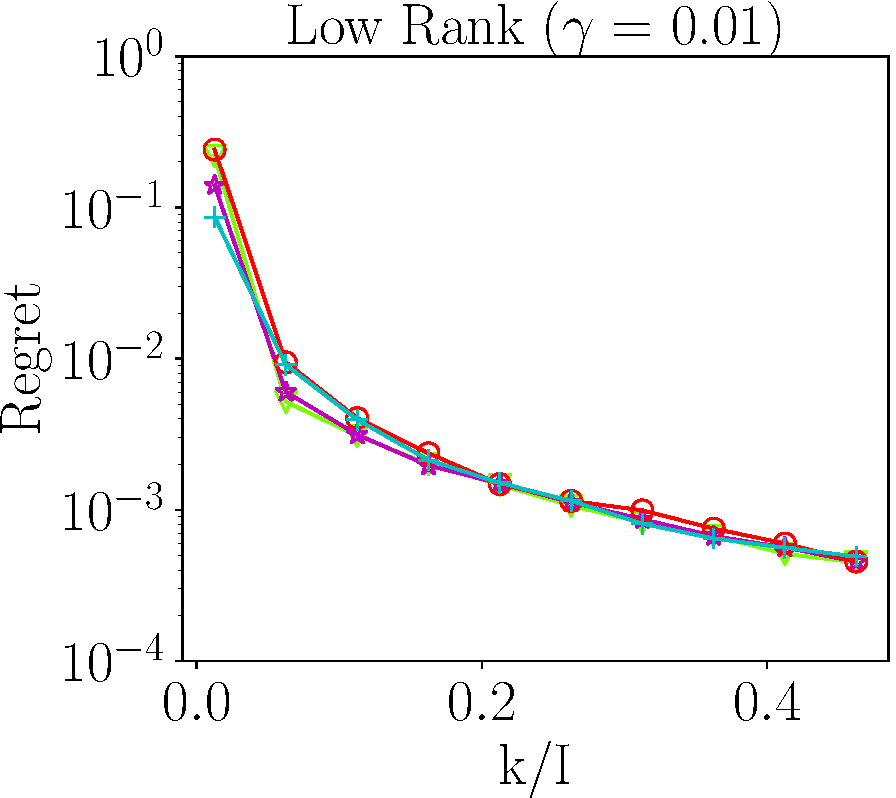
\includegraphics[scale = 0.24]{figure/fig2_lk_lnoise_400.pdf}
	\end{subfigure}
	\begin{subfigure}{0.3\textwidth}
		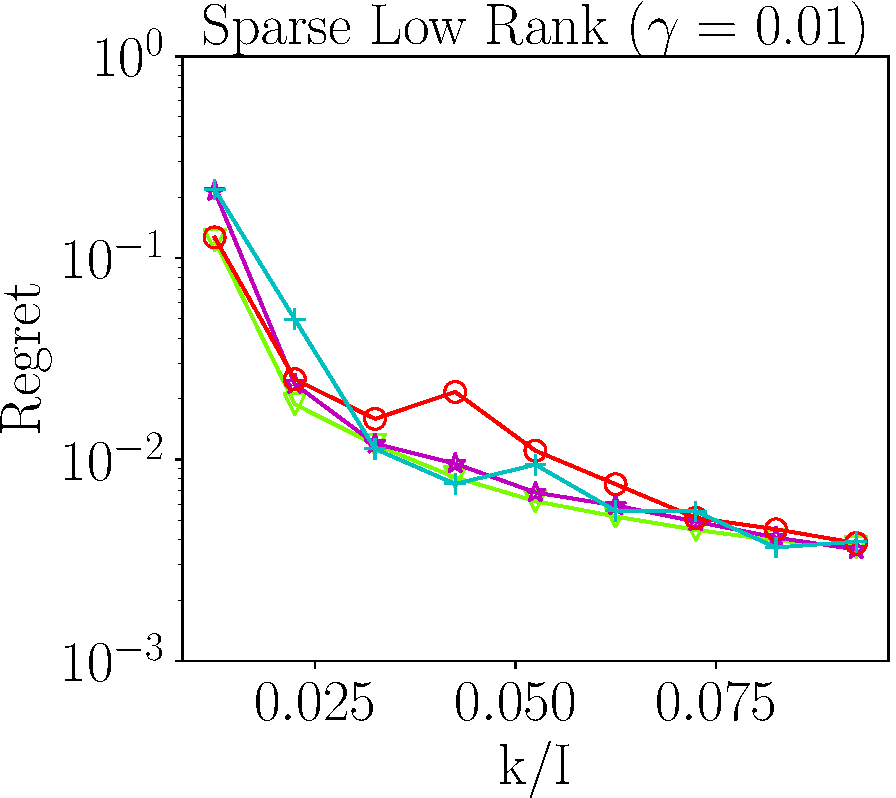
\includegraphics[scale = 0.24]{figure/fig2_slk_lnoise_400.pdf}
	\end{subfigure}
	\begin{subfigure}{0.3\textwidth}
		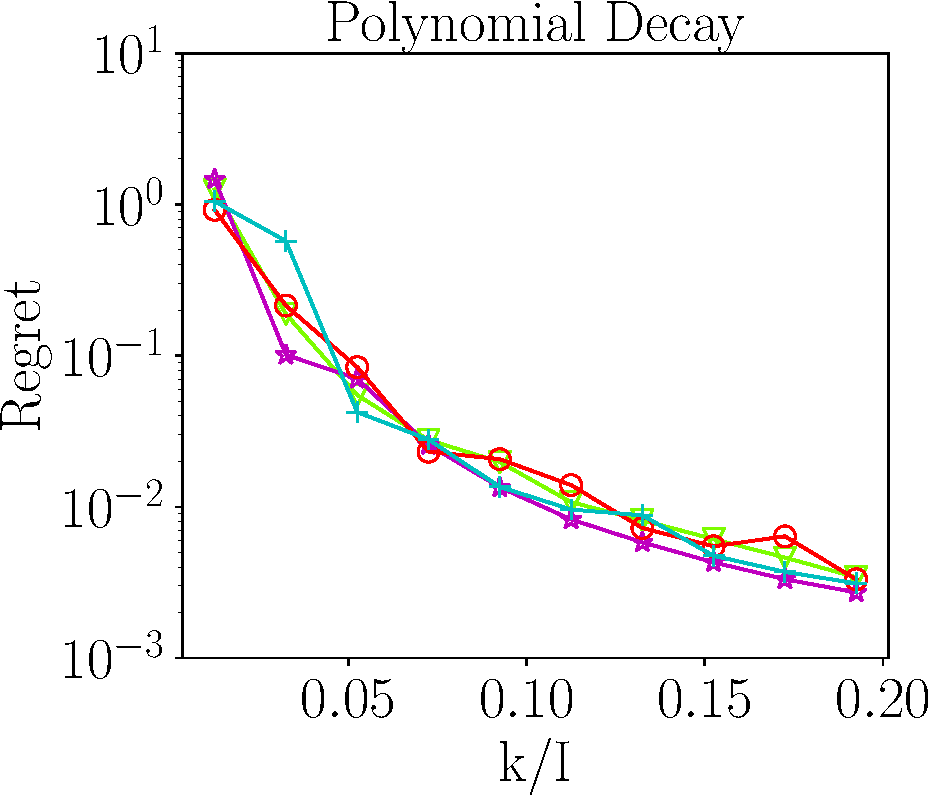
\includegraphics[scale = 0.24]{figure/fig2_spd_400.pdf}
	\end{subfigure}\\
	\begin{subfigure}{0.3\textwidth}
		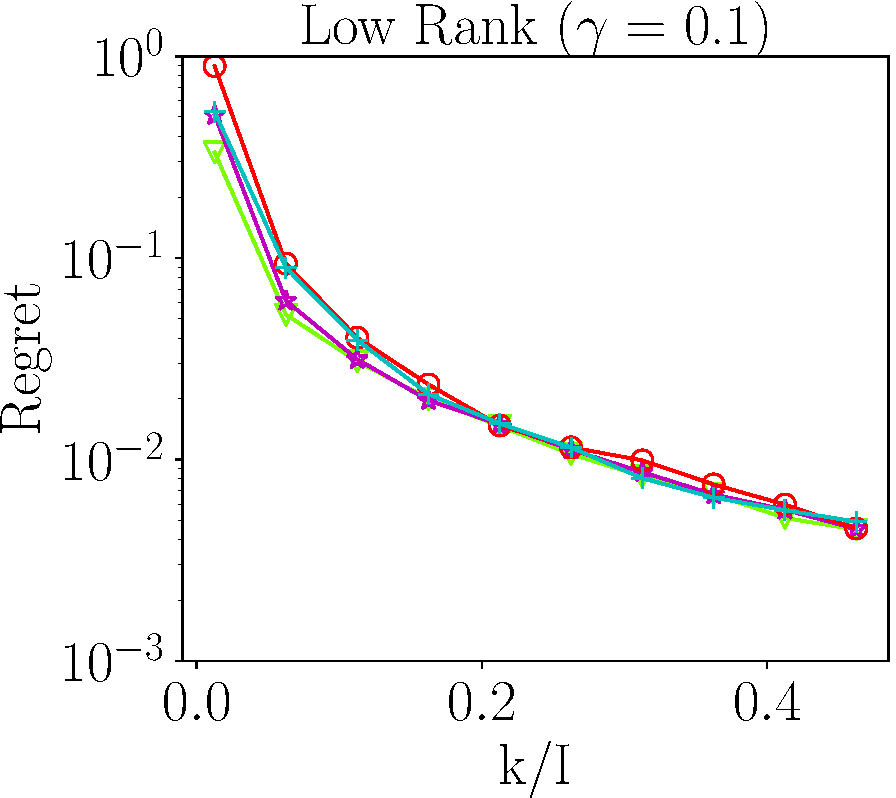
\includegraphics[scale = 0.24]{figure/fig2_lk_mnoise_400.pdf}
	\end{subfigure}
	\begin{subfigure}{0.5\textwidth}
		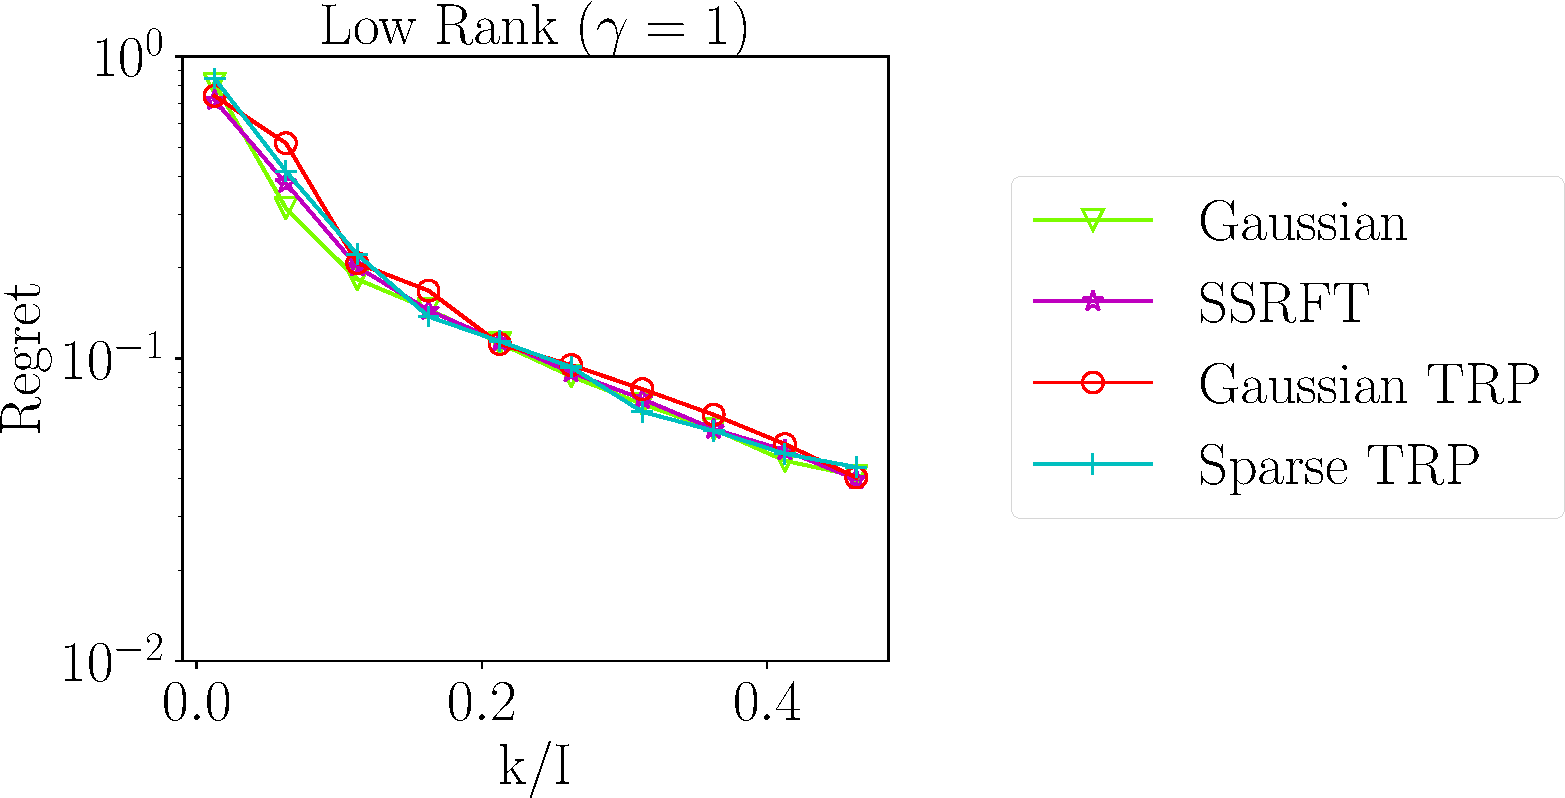
\includegraphics[scale = 0.24]{figure/fig2_lk_hnoise_400.pdf}
	\end{subfigure}
	\caption{We approximate 3D synthetic tensors (see \ref{s-synthetic-data}) with $I = 400$,
		using our one-pass algorithm with $r = 5$ and varying $k$ ($s = 2k+1$),
		using a variety of DRMs in the Tucker sketch:
		Gaussian, SSRFT, Gaussian TRP, or Sparse TRP.}
		\label{fig:vary-k-400-app}
\end{figure}



\begin{figure}
	\centering
	\begin{subfigure}{0.3\textwidth}
		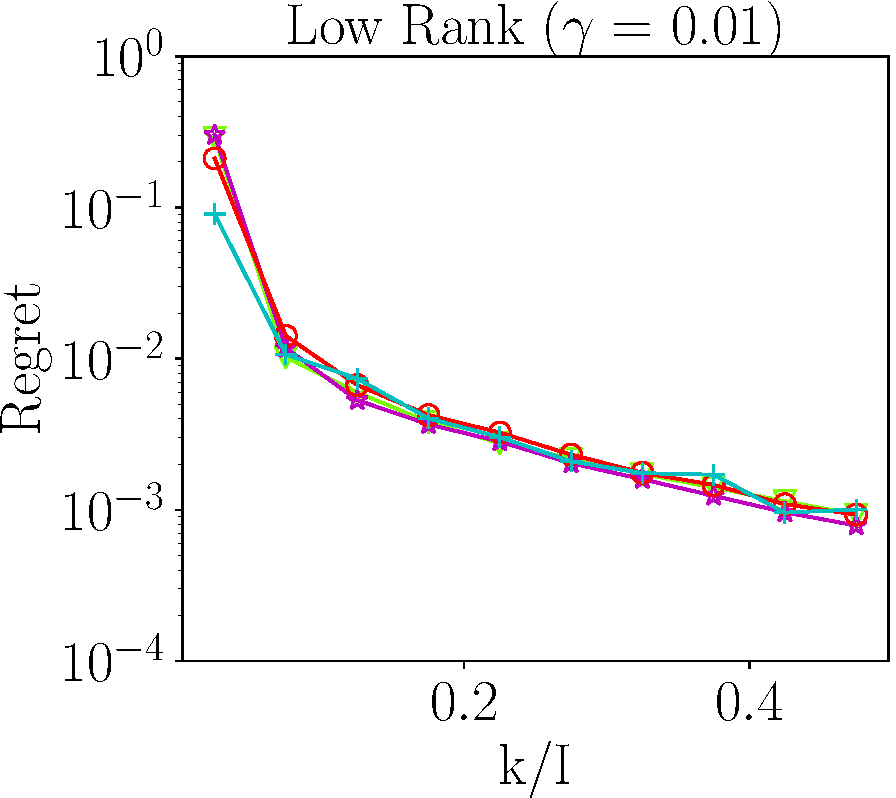
\includegraphics[scale = 0.25]{figure/fig2_lk_lnoise_200.pdf}
	\end{subfigure}
	\begin{subfigure}{0.3\textwidth}
		\includegraphics[scale = 0.25]{figure/fig2_slk_lnoise_200.pdf}
	\end{subfigure}
	\begin{subfigure}{0.3\textwidth}
		\includegraphics[scale = 0.25]{figure/fig2_spd_200.pdf}
	\end{subfigure}\\
	\begin{subfigure}{0.3\textwidth}
	\includegraphics[scale = 0.25]{figure/fig2_lk_mnoise_200.pdf}
	\end{subfigure}
	\begin{subfigure}{0.55\textwidth}
		\includegraphics[scale = 0.25]{figure/fig2_lk_hnoise_200.pdf}
	\end{subfigure}
	\caption{We approximate 3D synthetic tensors (see \ref{s-synthetic-data}) with $I = 200$,
		using our one-pass algorithm with $r = 5$ and varying $k$ ($s = 2k+1$),
		using a variety of DRMs in the Tucker sketch:
		Gaussian, SSRFT, Gaussian TRP, or Sparse TRP.}
		\label{fig:vary-k-200-app}
\end{figure}

% More comparison for two-pass and one-pass algorithm


\begin{figure}
	\centering
	\begin{subfigure}{0.3\textwidth}
		\includegraphics[scale = 0.24]{figure/fig3_lk_lnoise_400.pdf}
	\end{subfigure}
	\begin{subfigure}{0.3\textwidth}
		\includegraphics[scale = 0.24]{figure/fig3_slk_lnoise_400.pdf}
	\end{subfigure}
	\begin{subfigure}{0.3\textwidth}
		\includegraphics[scale = 0.24]{figure/fig3_spd_400.pdf}
	\end{subfigure}\\
	\begin{subfigure}{0.3\textwidth}
		\includegraphics[scale = 0.24]{figure/fig3_lk_mnoise_400.pdf}
	\end{subfigure}
	\begin{subfigure}{0.55\textwidth}
		\includegraphics[scale = 0.24]{figure/fig3_lk_hnoise_400.pdf}
	\end{subfigure}
	\caption{We approximate 3D synthetic tensors (see \ref{s-synthetic-data}) with $I = 400$,
		using our one-pass and two-pass algorithms with $r = 5$ and varying $k$ ($s = 2k+1$),
		using the Gaussian TRP in the Tucker sketch.}\label{fig:vary-k-400-compare-app}
\end{figure}



\begin{figure}
	\centering
	\begin{subfigure}{0.3\textwidth}
		\includegraphics[scale = 0.25]{figure/fig3_lk_lnoise_200.pdf}
	\end{subfigure}
	\begin{subfigure}{0.3\textwidth}
		\includegraphics[scale = 0.25]{figure/fig3_slk_lnoise_200.pdf}
	\end{subfigure}
	\begin{subfigure}{0.3\textwidth}
		\includegraphics[scale = 0.25]{figure/fig3_spd_200.pdf}
	\end{subfigure}\\
	\begin{subfigure}{0.3\textwidth}
		\includegraphics[scale = 0.25]{figure/fig3_lk_mnoise_200.pdf}
	\end{subfigure}
	\begin{subfigure}{0.55\textwidth}
		\includegraphics[scale = 0.25]{figure/fig3_lk_hnoise_200.pdf}
	\end{subfigure}
	\caption{We approximate 3D synthetic tensors (see \ref{s-synthetic-data}) with $I = 200$,
		using our one-pass and two-pass algorithms with $r = 5$ and varying $k$ ($s = 2k+1$),
		using the Gaussian TRP in the Tucker sketch.}\label{fig:vary-k-200-compare-app}

\end{figure}

% \section{More Real Data Results}
\label{appendix:more_real_data_result}

We also provide more numerical results on real datasets in Figure \ref{fig:srfrad_burden_dust}.
\begin{figure}[ht]
	\centering
	\includegraphics[height=2.9cm]{figure/multi_SRFRAD_frk8.pdf}
	\includegraphics[height=2.9cm]{figure/multi_SRFRAD_frk10.pdf}
	\includegraphics[height=2.9cm]{figure/multi_SRFRAD_frk15.pdf}\\
	\textbf{Net Radiative Flux at Surface}\\~\\
	\centering
	\includegraphics[height=2.9cm]{figure/multi_BURDENDUST_frk8.pdf}
	\includegraphics[height=2.9cm]{figure/multi_BURDENDUST_frk10.pdf}
	\includegraphics[height=2.9cm]{figure/multi_BURDENDUST_frk15.pdf}\\
	\textbf{Dust Aerosol Burden}
	\caption{We approximate the net radiative flux and dust aerosol burden data using our one-pass and two-pass algorithms using Gaussian TRP. We compare the performance under different ranks ($r/I = 0.125,0.2,0.067$). The dataset comes from the CESM CAM. The dust aerosol burden measures the amount of aerosol contributed by the dust. The net radiative flux determines the energy received by the earth surface through radiation. } \label{fig:srfrad_burden_dust}
\end{figure}

\end{subappendices}
\clearpage 
\chapter{Tensor Random Projection for Low Memory Dimension Reduction}

\section{Introduction}
Linear random projection is  operating a random matrix onto the data which could be either high dimension vector or matrix to reduce the dimension while preserving the useful information residing in the data. Then a linear random projection can be represented as a random matrix $\mathbf{\Omega}\in \real^{d\times k}$, operating on a vector $\mathbf{x}\in \real^{d}$ or a matrix $\mathbf{X} \in \real^{m\times d}$ to reduce the dimension:
\begin{equation}
\label{eq:low_dim_mapping}
\begin{aligned}
&\mathbf{x} \in \real^{n} \rightarrow  \mathbf{\Omega}^\top \mathbf{x} \in \real^{k} \\
& \mathbf{X} \in \real^{m\times d} \rightarrow   \mathbf{X}\mathbf{\Omega} \in \real^{m\times k}. 
\end{aligned}
\end{equation}

Random projection application to vector has a very long history which enables a broad range of modern applications from bio-informatics, informational retrieval to computer vision like \cite{wright2009robust,buhler2002finding,allen2014sparse,bingham2001random,fradkin2003experiments, halko2011finding, wang2012semi, jegou2008hamming}. In the context of large-scale relational databases, these maps enable
applications like information retrieval \cite{papadimitriou2000latent},
similarity search \cite{sahin2005prism,kaski1998dimensionality},
and privacy preserving distributed data mining \cite{liu2006random}. 
Later, along with the fast development in randomized algorithm, linear random projections are widely employed in constructing fast randomized algorithms in fields like matrix and tensor decomposition \cite{woolfe2008fast, tropp2017practical}, optimization \cite{yurtsever2017sketchy}, streaming data compression \cite{Tropp2019-SketchingScientificSimulation, sun2019low}. The much smaller matrix after random projection in the second line in \eqref{eq:low_dim_mapping} is named \emph{sketch}.  
The term 'sketch' describes the fact that the matrix after random projection captures most of the action of the original matrix.  \par 
The effectiveness of random projection is measured by whether the information inside data is well preserved in the low dimensional embedding after random projection. For the case where we operates random matrix $\mathbf{\Omega}$ onto vector $\mathbf{x}$, we require 
\begin{equation}
\|\mathbf{\Omega}^\top\mathbf{x}_1 - \mathbf{\Omega}^\top\mathbf{x}_2\| \approx 
\|\mathbf{x}_1 -\mathbf{x}_2\|.
\end{equation}
For the case, where we operating $\mathbf{\Omega}$ onto matrix $\mathbf{X}$, it requires that
\begin{equation}
\|\mathbf{QQ}^\top \mathbf{X} - \mathbf{X}\| ~ \text{is small}, 
\end{equation}
where $\mathbf{Q}$ is the ortho-normal matrix got from QR factorization from $\mathbf{X\Omega}$.
For the case where $\mathbf{\Omega}$ has i.i.d. elements, there are many literature in how these two properties are preserved. We list two well known results in literature for those two cases separately.  
\begin{lem}[\citet{arriaga2006algorithmic}]
	\label{lem:gauss-rp-vector}
	Let $\mathbf{x} \in \real^d$, assume that the entries in $\mathbf{\Omega}\in \real^{d\times k}$ are sampled independently from $\mathcal{N}(0, 1)$. Then
	\begin{equation}
	\label{eq:gauss_random_projection}
	\Prob\left((1-\epsilon)\|\mathbf{x}\|^2 \le \left\|\frac{1}{\sqrt{k}} \mathbf{\Omega}^\top \mathbf{x}\right\|\le (1+\epsilon)\|\mathbf{x}\|^2\right)\le 1 - 2e^{-(\epsilon^2-\epsilon^3)k/4}.
	\end{equation}
\end{lem}

\begin{lem}[\citet{halko2011finding}]
	\label{lemma:gauss-rp-matrix}
	Let $\mathbf{X} \in \real^{m\times d}$, assume that the entries in $\mathbf{\Omega}\in \real^{d\times (k+p)}$ are sampled independently from $\mathcal{N}(0, 1)$. Then let  $\mathbf{Q}$  
	be the orthonormal matrix  from QR factorization $\mathbf{X\Omega} = \mathbf{QR}$, then 
	\begin{equation}
	\label{eq:gauss_col_preservation}
	 \|\mathbf{X} - \mathbf{QQ}^\top \mathbf{X}\|_F \le \left(1+\frac{k}{p-1}\right)^{1/2}\left(\sum_{j>k} \sigma_j^2\right)^{1/2}.
	\end{equation}
\end{lem}


\paragraph{Memory Efficient Random Projection}
Sparse random maps for low memory dimension reduction
were first proposed by \cite{achlioptas2003database}, 
and further work has improved the memory requirements and guarantees of these methods
\cite{li2006very, ailon2006approximate, bourgain2015toward}.  Usually they propose the random projection to be sparse.  But under modern 'big data' setting, their cost in storage/memory cost is still to big to be practical. Consider





Most closely related to our work is Rudelson's foundational study \cite{rudelson2012row},
which considers how the spectral and geometric properties of
the random maps we use in this paper resemble a random map with iid entries,
and shows that their largest and smallest singular values are of the same order.
These results have been widely used to obtain guarantees for algorithmic privacy,
but not for random projection.
Battaglino et al. \cite{battaglino2018practical} use random projections
of Khatri-Rao products to develop a randomized least squares algorithm
for tensor factorization;
in contrast, our method uses the (full) Khatri-Rao product to enable random projection.
Sparse random projections to solve least squares problems were
also explored in \cite{wang2015fast} and \cite{woodruff2014sketching}.
To our knowledge, this paper is the first to consider using the Khatri-Rao product
for low memory random projection.
However, if the dimension of vectors before reduction
(here, the size of the lexicon) is too big,
the storage cost of the random map is not negligible.
Furthermore, even generating the pseudo-random numbers used to produce the random projection
is expensive \cite{matsumoto1998mersenne}.

To reduce the storage burden, we propose a novel use of the row-product random matrices in random projection, and call it the \textit{Tensor Random Projection} (TRP),
formed as the Khatri-Rao product of a list of smaller dimension reduction maps.
We show this map is an approximate isometry, with tunable accuracy,
and hence can serve as a useful dimension reduction primitive.
Furthermore, the storage required to compress $d$ dimension vectors scales as $\sqrt[N]d$
where $N$ is the number of smaller maps used to form the TRP.
We also develop a reduced variance version of the TRP that allows separate control
of the dimension of the range and the quality of the isometry.





\subsection{Notation}
We denote \textit{scalar}, \textit{vector}, and \textit{matrix} variables, respectively,
by lowercase letters ($x$), boldface lowercase letters ($\mathbf{x}$),
and boldface capital letters  ($\mathbf{X}$).
Let $[N] = \{1, \dots, N\}$.
For matrix $\mathbf{X}$, we denote its $i^{th}$ row, $j^{th}$ column, and the $(i,j)^{th}$ element as $\mathbf{X}_{(i,.)}, \mathbf{X}_{(.,j)}, \mathbf{X}_{(i,j)}$. The \textit{Kronecker product} of two matrices $\mathbf{A}\in \mathbb{R}^{m\times n},\mathbf{B} \in \mathbb{R}^{p\times q}$, denoted as $\mathbf{A} \otimes \mathbf{B} \in \mathbb{R}^{mp\times nq}$, is defined as 
\[
\mathbf{A} \otimes \mathbf{B} = \left[
\begin{array}{ccc}
A_{11}\mathbf{B}   & \cdots & A_{1n}\mathbf{B} \\
\vdots & \ddots & \vdots \\
A_{m1}\mathbf{B} & \cdots &   A_{mn}\mathbf{B}
\end{array}
\right].
\]
We let $\mathbf{X} \odot \mathbf{Y}$ denotes the \textit{Khatri-Rao product}, $\mathbf{A} \in \mathbb{R}^{I \times K}, \mathbf{B} \in \mathbb{R}^{J \times K}$, i.e. the "matching column-wise" Kronecker product. The resulting matrix of size $(IJ) \times K$ is given by: 
\begin{equation}\label{khatri-rao}
\mathbf{A} \odot \mathbf{B} = [\mathbf{A}_{(1,.)} \otimes \mathbf{B}_{(1,.)}, \dots, \mathbf{A}_{(K, .)} \otimes \mathbf{B}_{(K,.)}].
\end{equation}

\section{Tensor Random Projection}
We seek a random projection map to embed a collection of vectors
$\mathcal X \subseteq \mathbb{R}^{d}$
into $\mathbb{R}^k$ with $k \ll d$.
Let us take $d = \prod_{n=1}^N d_n$, motivated by the problem of compressing
(the vectorization of) an order $N$ tensor with dimensions $d_1,\ldots,d_N$. Conventional random projections use $O(kd)$ random variables.
Generating so many random numbers is costly; and storing them can be costly when $d$ is large.
Is so much randomness truly necessary for a random projection map?

% Indeed, we show it is not.
To reduce randomness and storage requirements, we propose
the \emph{tensor random projection} (TRP):
\begin{equation}
\label{eq:TRP}
f_{\text{TRP}}(\mathbf{x}):= (\mathbf{A}_1 \odot \cdots \odot \mathbf{A}_N)^\top
\mathbf{x},
\end{equation}
where each $\mathbf{A}_i \in \mathbb{R}^{d_i \times k}$, for $i \in [N]$,
can be an arbitrary RP map and
$\mathbf{A} := (\mathbf{A}_1 \odot \cdots \odot \mathbf{A}_N)^\top$.
We call $N$ the \emph{order} of the TRP.
% This construction is inspired by the CANDECOMP/PARAFAC (CP) decomposition in
% low-rank tensor approximation \cite{kolda2009tensor}.
We show in this paper that the TRP is an expected isometry,
has vanishing variance,
and supports database-friendly operations.
%For more background knowledge about tensor decomposition, please refer to \cite{kolda2009tensor}.

The TRP requires only $k\sum_{i = 1}^N d_i$ random variables
(or $k\sqrt[N]{d}$ by choosing each $d_i$ to be equal),
rather than the $kd$ random variables needed by conventional methods.
Hence the TRP is database friendly:
it significantly reduces storage costs and randomness requirements compared to its
constituent DRMs.

In large scale database settings,
where computational efficiency is critical and queries of vector elements are costly,
practitioners often use sparse RPs.
Let $\delta$ be the proportion of non-zero elements in the RP map.
To achieve a $\delta$-sparse RP, a common construction is the scaled sign random map:
each element is distributed as $(-1/\sqrt{\delta}, 0, 1/\sqrt{\delta})$ with probability
$(\delta/2, 1-\delta, \delta/2)$.
\cite{achlioptas2003database} proposed $\delta=1/3$,
while \cite{li2006very} further suggests a sparser scheme with
$\delta=1/\sqrt{d}$ that he calls the \textit{Very Sparse} RP.

To further reduce memory requirements of random projection,
we can form a TRP whose constituent submatrices
are generated each with sparsity factor $\delta$,
which leads to a $\delta^N$-sparse TRP. Under sparse setting, it is a $(1/3)^N$ sparse TRP while under very sparse setting, it is a $1/\sqrt{d}$ sparse TRP. 
Both TRPs can be applied to a vector using very few queries to vector elements
and no multiplications.
Below, we show both sparse and very sparse TRP are low-variance approximate isometry empirically. 

\section{Main Theory}
In this section, we discuss the properties of tensor random projection with application to length preservation and column space preservation.  


\subsection{Bias and Variance}
In this section, we will show the TRP and $\textup{TRP}_T$ are expected isometries with vanishing variance.
We provide a rate for the decrease in variance with $k$.
We also prove a non-asymptotic concentration bound on the quality of the isometry when $N=2$.
%but leave the task of building concentration bound for $N\ge 3$ case for the future exploration.
We begin by showing the TRP is an approximate isometry.
\begin{thm}
\label{thm: norm-preserve}
Fix $\mathbf{x} \in \mathbb{R}^{\prod_{n=1}^N d_n}$.
Form a TRP and $\textup{TRP}_T$ of order $N$ with range $k$
composed of independent matrices with independent columns
whose entries are mean zero, variance one, and within each column every pair of elements has covariance zero.
Then
\begin{equation}
\label{eq:lemma-invariant-length-statement}
\E \|\textup{TRP}(\mathbf{x})\|^2 = \|\mathbf{x}\|^2 \qquad \text{and} \qquad  \mathbb{E} \|
\textup{TRP}_T(\mathbf{x})\|^2 = \|\mathbf{x}\|^2. \nonumber
\end{equation}
\end{thm}
Interestingly, Theorem \ref{thm: norm-preserve} does not require elements of $\mathbf{A}_n$ to be iid.
Now we present an explicit form for the variance of the isometry.
\begin{thm}
\label{thm:variance}
Fix $\mathbf{x} \in \mathbb{R}^{\prod_{n=1}^N d_n}$.
Form a \textup{TRP} and $\textup{TRP}_T$ of order $N$ with range $k$
independent matrices whose entries are i.i.d. with
mean zero, variance one, and fourth moment $\Delta$.
Then
\begin{equation*}
\begin{aligned}
% &\textrm{Var}(\|\textup{TRP}(\mathbf{x})\|^2) = \frac{1}{k}\left[ (\Delta^N-3)\|\mathbf{x}\|_4^4 +2\|\mathbf{x}\|_2^4\right] ,\\
% &\textrm{Var}(\|\textup{$\textup{TRP}_T$}(\mathbf{x})\|^2) = \frac{1}{Tk}(\Delta^N-3)\|\mathbf{x}\|_4^4 + \frac{2}{k}\|\mathbf{x}\|_2^4.
% \end{aligned}
& \var(\|\textup{TRP}(\mathbf{x})\|^2) = \frac{1}{k}(\Delta^N-3)\|\mathbf{x}\|_4^4 + \frac{2}{k}\|\mathbf{x}\|_2^4 \\
& \var(\|\textup{TRP}_T(\mathbf{x})\|^2) = \frac{1}{Tk}(\Delta^N-3)\|\mathbf{x}\|_4^4 + \frac{2}{k}\|\mathbf{x}\|_2^4.
\end{aligned}
\end{equation*}
\end{thm}
We can see the variance increases with $N$.
In the $N=1$ Gaussian case, this formula shows a variance of $2/k \|\mathbf{x}\|_2^4$,
which agrees with the classic result.
Notice the $\textup{TRP}_T$ only reduces the first term in the variance bound:
as $T\rightarrow \infty$, the variance converges to that of a Gaussian random map.\par 

Next, since $\textup{TRP}_T$ is a linear operator, treat $\mathbf{x}-\mathbf{y}$ as a vector, with above argument,  we have the following lemma for pair-wise distance.  Proof is omitted for the sake of brevity. 

\begin{cor}\label{cor:pairwise-distance-unbias-variance} 
	Fix $\mathbf{x}, \mathbf{y} \in \mathbb{R}^{\prod_{n=1}^N d_n}$. Form a $\textup{TRP}_T$ of order $N$ with range $k$ independent matrices whose entries are i.i.d with mean zero, variance one, and fourth moment $\Delta$. We have
	\begin{equation}
	\begin{aligned}
	&\mathbb{E} (\|\textup{TRP}_T(\mathbf{x}) - \textup{TRP}_T(\mathbf{y})\|^2) = \|\mathbf{x}-\mathbf{y}\|^2,  \\ 
	&\var(\|\textup{TRP}_T(\mathbf{x}) - \textup{TRP}_T(\mathbf{y})\|^2) = \frac{1}{Tk}(\Delta^N-3)\|\mathbf{x} - \mathbf{y} \|_4^4 + \frac{2}{k}\|\mathbf{x}-\mathbf{y}\|_2^4. 
	\end{aligned}
	\end{equation}
\end{cor}


For completeness,  we also present the analysis for bias and variance for inner product. 

\begin{lem} \label{lem:inner_product_TRP}
	Fix $\mathbf{x}, \mathbf{y} \in \mathbb{R}^{\prod_{n=1}^N d_n}$. For $\textup{TRP}$ and $\textup{TRP}_T$ of order $N$ with range $k$ independent matrices whose entries are i.i.d with mean zero, variance one, and fourth moment $\Delta$, we have 
	\begin{equation}
	\begin{aligned}
	 \mathbb{E} (\langle \textup{TRP}(\mathbf{x}), \textup{TRP}(\mathbf{y}) \rangle) &= \mathbb{E} (\langle \textup{TRP}_T(\mathbf{x}), \textup{TRP}_T(\mathbf{y}) \rangle) = \langle \mathbf{x}, \mathbf{y}\rangle  \\ 
	 \var(\langle \textup{TRP}(\mathbf{x}), \textup{TRP}(\mathbf{y}) \rangle) &=\frac{1}{k} [ (\Delta^N - 3) \sum_{\mathbf{r}}x_{\mathbf{r}}^2y_{\mathbf{r}}^2  + \|\mathbf{x}\|_2^2\|\mathbf{y}\|^2_2 + \langle \mathbf{x}, \mathbf{y} \rangle^2].\\ 
	\var(\langle \textup{TRP}_T(\mathbf{x}), \textup{TRP}_T(\mathbf{y}) \rangle) &= \frac{1}{kT}(\Delta^N -3) \sum_{\mathbf{r}}x_{\mathbf{r}}^2y_{\mathbf{r}}^2 +  (\frac{2}{k} - \frac{1}{kT})\|\mathbf{x}\|_2^2\|\mathbf{y}\|_2^2 + \frac{1}{kT}\langle \mathbf{x}, \mathbf{y} \rangle^2. 
	\end{aligned}
	\end{equation}
\end{lem}

We can see as $T \rightarrow \infty$, $	\var(\langle \textup{TRP}_T(\mathbf{x}), \textup{TRP}_T(\mathbf{y}) \rangle) \rightarrow \frac{2}{k}\|\mathbf{x}\|_2^2\|\mathbf{y}\|_2^2$, same as the variance in the Gaussian Random map case. 

\begin{remark}
If we further assume each entry of $\mathbf{x}, 
\mathbf{y}$ to be a random variable with their second and fourth moment bounded by constants. We can see as $d \rightarrow \infty$,  $\|\mathbf{x}\|_2^4$,  $\|\mathbf{x}\|_2^2\|\mathbf{y}\|_2^2$, $\langle \mathbf{x},\mathbf{y} \rangle^2$ are $\mathcal{O}(d^2)$, and $\|\mathbf{x}\|_4^4$, $\sum_{\mathbf{r}}x^2_{\mathbf{r}}y^2_{\mathbf{r}}$ are $\mathcal{O}(d)$ respectively. Thus, $\frac{2}{k}\|\mathbf{x}\|_2^4$, i.e. the term same as in the Gaussian RP, dominates $\var(\|\textup{TRP}(\mathbf{x})\|^2)$, and $\frac{1}{k}(\|\mathbf{x}\|_2^2\|\mathbf{y}\|_2^2 + \langle \mathbf{x}, \mathbf{y} \rangle^2)$ dominates $\var(\langle \textup{TRP}(\mathbf{x}), \textup{TRP}(\mathbf{y}) \rangle )$. 
\end{remark}

\subsection{Asymptotic Behavior}


\subsection{Finite Sample Bound?}
Finally we show a non-asymptotic concentration bound for $N=2$.
We leave the parallel result for $N\ge 3$ open for future exploration.


\begin{prop}
	\label{prop: N-2-bound}
	Fix $\mathbf{x} \in \mathbb{R}^{d_1 d_2}$ with sub-Gaussian norm $\varphi_2$.
	Form a \textup{TRP}(T) of order 2 with range $k$
	composed of two independent matrices whose entries are drawn i.i.d.
	from a sub-Gaussian distribution with mean zero and variance one.
	Then there exists a constant $C$ depending on $\varphi_2$
	and a universal constant $c_1$ % XXX universal? or what?
	so that
	\begin{equation}
	\mathbb{P}\left(\left| \|f_{\textup{TRP}}(\mathbf{x})\|^2 - \|\mathbf{x}\|^2_2 \right| \ge \epsilon \|x\|^2\right)\le C\exp\left[ - c_1 \left(\sqrt{k}\epsilon\right)^{1/4} \right],\nonumber
	\end{equation}
	
\end{prop}
Here $\varphi_2$ is the sub-Gaussian norm defined in \ref{def:sub-gaussian} in Appendix \ref{sec:appendix_proof}.
\ref{prop: N-2-bound} shows that for a TRP to form an $\epsilon$-JL DRM
with substantial probability on a dataset with $n$ points,
our method requires $k=\mathcal{O}(\epsilon^{-2}\log^8 n)$ while
conventional random projections require $k=\mathcal{O}(\epsilon^{-2}\log n)$.
Numerical experiments suggest this bound is pessimistic.
\subsection{Column Space Preservation}
\eqref{eq:gauss_col_preservation} in Lemma \ref{lemma:gauss-rp-matrix} shows that the random projection preserve the information in column space of a matrix well and provide the error bound compared with the tail energy. It is hard to derive similar result for general matrix with tensor random projection. But if the matrix is in form of kroneck product, we can get a similar result based as following proposition:
\begin{prop}
Let $\M{X}_n\in \mathbb{R}^{m_i\times d_n}$ be a series of matrix and $\M{\Omega}_n\in \mathbb{R}^{d_n\times (k+p_n)}$ with eact element sampled from standard Gaussian distribution, let  $\tau_n(k) = \sum_{j>k} \sigma^2_j(\M(x))$ be the tail energy for $\M{X}_i$. Let $\M{Q}\in \mathbb{R}^{d\times k}$ be the orthonormal matrix from QR factorization: 
\[
\M{Q}, - = \rm{QR} [(\M{X}_1\otimes \cdots \otimes \M{X}_N)(\M{\Omega}_1\odot \cdots \odot\M{\Omega}_N)]
\]
we have
\begin{equation}
\begin{aligned}
&\E \| (\M{X}_1\otimes \cdots \otimes \M{X}_N) - \M{QQ}^\top(\M{X}_1\otimes \cdots \otimes \M{X}_N)\|^2_F \\
& \le \prod_{i=1}^N  \left(1+\frac{k}{p_n-1}\right)\tau^2_n(k). 
\end{aligned}
\end{equation}
\end{prop}
\begin{proof}
\citep{schacke2013kronecker} has a detailed descriptions on properties for kronecker product. Here we mainly use the association rule between kronecker product and khatri rao product, which claims for $\M{A}\in \reals^{m_n\times d_n}$ 
and $\M{B}\in \reals^{d_n\times k}$
\begin{equation}
\begin{aligned}
& (\M{A}_1\otimes \cdots \otimes \M{A}_N)(\M{B_1} \odot \cdots \odot \M{B_N})  \\
& = ( \M{A}_1\M{B_1}\odot \cdots \odot  \M{A}_N\M{B}_N). 
\end{aligned}
\end{equation}
Also, for orthogonal matrix $\M{U}_n, n = 1, \cdots, N$, ($\M{U}^\top_n \M{U}_n = \M{I}$),  $\M{U}_1\odot $

Using this association rule,  
\begin{equation}
\begin{aligned}
& (\M{X}_1\otimes \cdots \otimes \M{X}_N)(\M{\Omega_1} \odot \cdots \odot \M{\Omega_N})  \\
& = ( \M{X}_1\M{\Omega_1}\odot \cdots \odot  \M{X}_N\M{\Omega_N}). 
\end{aligned}
\end{equation}
 Let $\M{Q}_n\in \mathbb{R}^{d_n\times k}$ be the orthonormal matrix from QR factorization: $\mathbf{Q}_i, - \gets  \rm{QR}(\M{X_i\Omega_i})$. The key observation is that 
 $\M{Q} = \M{Q}_1\otimes \cdots \otimes \M{Q}_N$ then we finish the proof with some association rule for kronecker product in \cite{schacke2013kronecker} and result in Lemma \ref{lemma:gauss-rp-matrix}.  Also this proposition, indicate in practice, we should sketch each small matrix $\M{X}_n$ then combine them together which is equivalent to do sketch the whole matrix after kronecker product. 
 
\end{proof}






\section{Experiment} \label{sec:simulation}
In this section, we compare the quality of the isometry of
conventional RPs, TRP, and TRP(5), for
Gaussian, Sparse \cite{achlioptas2003database},
and Very Sparse random maps \cite{li2006very} on both synthetic data and MNIST data.
We also use TRP and TRP(5) to compute pairwise cosine similarity
(Table \ref{tbl:mnist_inner_prod} and Appendix \ref{appendix:more_result})
and to sketch matrices and tensors
(Appendix \ref{appendix:sketching}),
although the theory still remains open.
% irrelevant, since we don't show timing
% We implemented the algorithm in Python and ran all experiments on a server with
% 128 Intel\textsuperscript{\textregistered} Xeon\textsuperscript{\textregistered} E7-4850
% v4 2.10GHz CPU cores and 1056GB memory.

Our first experiment evaluates the quality of the isometry for maps $\mathbb{R}^d \to \mathbb{R}^k$.
We generate $n=10$ independent vectors $\mathbf{x}_1, \dots, \mathbf{x}_n$ of sizes
$d = 2500, 10000, 40000$ from $\mathcal{N}(\mathbf{0},\mathbf{I})$.
We consider the following three RPs:
1. Gaussian RP; 2. Sparse RP \cite{achlioptas2003database}; 3. Very Sparse RP \cite{li2006very}.
For each, we compare the performance of RP, TRP, and TRP(5) with order 2 and $d_1=d_2$.
We evaluate the methods by repeatedly generating a RP and computing the reduced vector,
and plot the ratio of the pairwise distance
$\frac{1}{n(n-1)}\sum_{n \geq i\neq j \geq 1}\frac{\|\mathbf{A}\mathbf{x}_i - \mathbf{A}\mathbf{x}_j\|_2}{\|\mathbf{x}_i - \mathbf{x}_j\|_2}$
and the average standard deviation for different $k$
averaged over 100 replications.
In the MNIST example, we choose the first $n = 50$ vectors of size $d = 784$, normalize them,
and perform the same experiment.
Figure \ref{fig:main} shows results on simulated ($d = 2500$) and MNIST data
for the Gaussian and Very Sparse RP.
See \ref{appendix:more_result} for additional experiments.

These experiments show that to preserve pairwise distance and cosine similarity,
TRP performs nearly as well as RP for all three types of maps.
With only five replicates, TRP(5) reduces the variance significantly in real data while not much in the simulation setting.
The difference in accuracy between methods diminishes as $k$ increases.
When $d = d_1d_2 = 40000$, the storage for TRP(5) is still $\frac{1}{20}$ of the Gaussian RP.
The variance reduction is effective especially in sparse and very sparse setting.


\begin{figure}[H]
	\centering
	\begin{subfigure}{0.24\textwidth}
		\includegraphics[scale = 0.22]{figure/dist_g_d2500.pdf}
	\end{subfigure}
	\begin{subfigure}{0.24\textwidth}
		\includegraphics[scale = 0.22]{figure/dist_sp1_d2500.pdf}
	\end{subfigure}
	\begin{subfigure}{0.24\textwidth}
		\includegraphics[scale = 0.22]{figure/dist_g_mnist.pdf}
	\end{subfigure}
	\begin{subfigure}{0.24\textwidth}
		\includegraphics[scale = 0.22]{figure/dist_sp1_mnist.pdf}
	\end{subfigure}\\
	\caption{Isometry quality for simulated and MNIST data.
		The left two plots show results for Gaussian and Very Sparse RP, TRP, TRP(5)
		respectively applied to $n = 20$ standard normal data vectors in $\mathbb{R}^{2500}$.
		The right two plots show the same for 50 MNIST image vectors in $\mathbb{R}^{784}$.
		The dashed line shows the error two standard deviations from the average ratio.}
	\label{fig:main}
\end{figure}

\begin{table}[H]
	\centering
	\begin{tabular}{l|l|l|l}
		& Gaussian        & Sparse          & Very Sparse     \\ \hline
		RP & 0.1198 (0.0147) & 0.1198 (0.0150) & 0.1189 (0.0108) \\ \hline
		TRP    & 0.1540 (0.0290) & 0.1609 (0.0335) & 0.1662 (0.0307) \\ \hline
		TRP(5) & 0.1262 (0.0166) & 0.1264 (0.0194) & 0.1276 (0.0164)
	\end{tabular}
	\caption{RMSE for the estimate of the pairwise inner product of the MNIST data, where standard error is in the parentheses.} \label{tbl:mnist_inner_prod}
\end{table}
\section{Application: Sketching}
\label{appendix:sketching}
Beyond random projection, our novel TRP also has an important application in sketching. Sketching is an important technique to accelerate expensive computations with widespread applications, such as regression, low-rank approximation, and graph sparsification, etc. \citep{halko2011finding,woodruff2014sketching} 
% I have to think about how to argue tensor has a natural Khatri-Rao structure. 
The core idea behind sketching is to compress a large dataset, typically a matrix or tensor, into a smaller one by multiplying a random matrix. 
%Since the matrix multiplication is a linear operation, people can usually further extend sketching to distributed and online setting. 
In this section, we will mainly focus on the low-rank matrix approximation problem. Consider a matrix $\mathbf{X} \in \mathbb{R}^{m \times d}$ with rank $r$, 
we want to find the best rank-$r$ approximation with the minimal amount of time. The most common method is the randomized singular value decomposition (SVD), whose underlying idea is sketching. 


First, we compute the linear sketch $\mathbf{Z} \in \mathbb{R}^{m \times k}$ by $\mathbf{Z} =\mathbf{X}\mathbf{\Omega}$, where $\mathbf{\Omega} \in \mathbb{R}^{d \times r}$ is the random map. Then we compute the QR decomposition of $\mathbf{X}\mathbf{\Omega}$ by $\mathbf{Q}\mathbf{R} = \mathbf{Z}$, where $\mathbf{Q} \in \mathbb{R}^{m \times k}, \mathbf{R} \in \mathbb{R}^{r \times r}$. At the end, we project $\mathbf{X}$ onto the column space of $\mathbf{Q}$, and obtain the approximation $\hat{\mathbf{X}} = \mathbf{Q} \mathbf{Q}^\top \mathbf{X}$.  

With our TRP, we can significantly reduce the storage of the random map, while achieving similar rate of convergence as demonstrated in Figure \ref{fig:col_matrix}. 
With further variance reduction by taking the geometric-median over multiple runs, our TRP with variance reduction can achieve even better performance. The detailed implementation is given in Algorithm \ref{alg:var-red-structure-sketching}. And we will delay the theoretical analysis of this method for future works. 


\begin{algorithm}[H]
	\caption{Tensor Sketching with Variance Reduction}\label{alg:var-red-structure-sketching}
	\begin{algorithmic}[1]
		\Require $\mathbf{X} \in \mathbb{R}^{m \times d}$, where $d = \prod_{i=1}^N d_n$ and 
		\rm{RMAP} is a user-specified function that generates a random dimension reduction map. $T$ is the number of runs for variance reduction averaging. 
		\Function{SSVR}{$\mathbf{X}, \{d_n\}, k, T, \rm{RMAP}$}\\
		\text{For $t= 1 \dots T$}\\
		\text{For $i = 1 \dots N$} \\
		$\mathbf{\Omega}_i^{(t)} = \rm{RMAP}(d_i, k)$
		\State $\mathbf{\Omega}^{(t)} = \mathbf{\Omega}_1^{(t)} \odot \cdots \odot \mathbf{\Omega}_{N}^{(t)}$
		\State $(\mathbf{Q}^{(t)}, \sim ) = \rm{QR}(\mathbf{X}\mathbf{\Omega}^{(t)})$ 
		\State $\hat{\mathbf{X}}^{(t)} = \mathbf{Q}^{(t)}\mathbf{Q}^{(t)T}\mathbf{X}$
		\State
		$\hat{\mathbf{X}} = \frac{1}{T}\sum_{t=1}^T \hat{\mathbf{X}}^{(t)}$
		\State \Return $\mathbf{G}$
		\EndFunction
	\end{algorithmic}
\end{algorithm}

Furthermore, the extension of TRP to tensor data is also natural. To be specific, the $n^{th}$ unfolding of a large tensor $\mathscr{X} \in \mathbb{R}^{I_1 \times \cdots \times I_N}$, denoted as $\mathbf{X}^{(n)}$, has dimension $I_n \times I_{(-n)}$, where $I_{(-n)} = \prod_{i \neq n, i \in [N]} I_i$ . To construct a sketch for the unfolding, we need to create a random matrix of size $ I_{(-n)} \times k$. Then, our TRP becomes a natural choice to avoid the otherwise extremely expensive storage cost. For many popular tensor approximation algorithms, it is even necessary to perform sketching for every dimension of the tensor \citep{de2000multilinear,wang2015fast}. 
%such as Higher-Order Orthogonal Iteration \citep{de2000multilinear}, Fast CANDECOMP/PARAFAC decomposition \citep{wang2015fast}, our paper ? 
In the simulation section, we perform experiments for the unfolding of the higher-order order tensor with our structured sketching algorithms (Figure \ref{fig:col_matrix}). For more details in tensor algebra, please refer to \citep{kolda2009tensor}. 


\paragraph{Experimental Setup}
In sketching problems, considering a $N$-D tensor $\mathscr{X} \in \mathbb{R}^{I^N}$ with equal length along all dimensions, we want to compare the performance of the low rank approximation with different maps for its first unfolding $\mathbf{X}^{(1)} \in \mathbb{R}^{I \times I^{N-1}}$. 
	
We construct the tensor $\mathscr{X}$ in the following way. Generate a core tensor $\mathscr{C} \in \mathbb{R}^{r^N}$, with each entry $\rm{Unif}([0,1])$. Independently generate $N$ orthogonal arm matrices by first creating $\mathbf{A}_1, \dots, \mathbf{A}_N \in \mathbb{R}^{r \times I}$ and then computing the arm matrices by $(\mathbf{Q}_n, \sim) = \rm{QR}(\mathbf{A}_n)$, for $1 \leq n \leq N$.
\begin{equation}
\mathscr{X} = \mathscr{C} \times_1 \mathbf{Q}_1 \cdots \times_N \mathbf{Q}_N + \sqrt{\frac{0.01 \cdot \|\mathscr{X}^\natural\|_F^2}{I^N}} \mathcal{N}(0,1). \nonumber
\end{equation}
Then, we construct the mode-1 unfolding of $\mathbf{X} = \mathbf{X}^{(1)}$, which has a rank smaller than or equal to $r$. 

In our simulation, we consider the scenarios of 2-D ($900 \times 900$), 3-D ($400 \times 400 \times 400$), 4-D ($100 \times 100 \times 100 \times 100$) tensor data, with corresponding mode-1 unfolding of size $900 \times 900$, $400 \times 160000$, $100 \times 1000000$ respectively and $r = 5$. In each scenario, we compare the performance for Gaussian RP, TRP, and $\textup{TRP}_5$ maps with varying $k$ from 5 to 25. The TRP map in these scenarios has 2, 4, 6 components of size $30 \times k$, $20 \times k$, $10 \times k$ respectively. And the number of runs variance reduction averaging is $T = 5$. In the end, we evaluate the performance by generating the random matrix 100 times and compute the relative error $\frac{\|\mathbf{X} - \hat{\mathbf{X}}\|}{\|\mathbf{X}\|}$, and constructing a 95\% confidence interval for it.

\paragraph{Result}From Figure \ref{fig:col_matrix}, we can observe that the relative error decreases as $k$ increases as expected for all dimension reduction maps. The difference of the performance between the Khatri-Rao map and Gaussian map is small when $N = 2$, but increases when $N$ increases, whereas the Khatri-Rao variance reduced method is particularly effective producing strictly better performance than the other two. 

\begin{figure*}[ht!]
	\centering
	\begin{subfigure}{0.32\textwidth}
		\includegraphics[scale = 0.3]{figure/col_dim2_krao_d900.pdf}
	\end{subfigure}
	\begin{subfigure}{0.32\textwidth}
		\includegraphics[scale = 0.3]{figure/col_dim3_krao_d160000.pdf}
	\end{subfigure}
	\begin{subfigure}{0.32\textwidth}
		\includegraphics[scale = 0.3]{figure/col_dim4_krao_d1000000.pdf}
	\end{subfigure}\\
	\caption{Relative Error for the low-rank tensor unfolding approximation: \textit{we compare the relative errors for low-rank tensor approximation with different input size: 2-D ($900 \times 900$), 3-D ($400 \times 400 \times 400$), 4-D ($100 \times 100 \times 100 \times 100$). In each setting, we compare the performance of Gaussian RP, TRP, and $\textup{TRP}_5$. The dashed line stands for the 95\% confidence interval.}}
	\label{fig:col_matrix}
\end{figure*}


\section{Conclusion}
The TRP is a novel dimension reduction map composed of smaller DRMs.
Compared to its constituent DRMs, it significantly reduces
the requirements for randomness and for storage.
% and computation cost (number of access to database), % XXX not sufficiently justified
Numerically, the variance-reduced TRP(5) method with only five replicates
achieves accuracy comparable to the conventional RPs for $1/20$ of the original storage.
We prove the TRP and TRP(T) are expected isometries with vanishing variance,
and provide a non-asymptotic error bound for the order 2 TRP.

% Can delete any of this
%to derive the central limit theorem
%for estimator pair-wise distance, and 
For the future work, we will provide a general non-asymptotic bound
for the higher order TRP 
%and to explore other methods for variance reduction using ideas from robust statistics.
and develop the theory relevant for the application of the TRP
in sketching low-rank approximation, given its practical effectiveness
(shown in Appendix \ref{appendix:sketching}).


\begin{subappendices}
\section{Proof for Bias and Variance Analysis}
\label{sec:appendix_proof}


Before presenting the proof for the main theory, we first define some new notations. Since these notations will only be used in technical proofs, we do not include them in the main body. 

\subsection*{Extra Notations for Technical Proofs} 
For a vector $\mathbf{x}$ with length $\prod_{n=1}^N d_n$, for simplicity, we introduce the multi-index for it: let $\mathbf{x}_{r_1, \cdots, r_N},\forall r_n \in [d_n]$, represent the $(1 + \sum_{n = 1}^N(r_n -1)s_n)^{th}$ element, where $s_n = \prod_{n+1}^Nd_n$ for $n < N$, and $1$ for $n = N$. For vector $\mathbf{r}_1$, $\mathbf{r}_2$, we say $\mathbf{r}_1 = \mathbf{r}_2$ if and only if 
all their elements are the same. 
\par 

Also, we let $\mathop{\mathbf{vec}}(\mathbf{A})$ be the vectorization operator for any matrix $\mathbf{A}\in \mathbb{R}^{d\times k}$, which stacks all columns of matrix $\mathbf{A}$ and returns a vector of length $kd$, 
$[\mathbf{A}(\cdot, 1); \cdots; \mathbf{A}(\cdot, k); ]$. Here we use semi-colon to denote the vertical stack of vectors $\mathbf{x}$ and $\mathbf{y}$ as $[\mathbf{x}; \mathbf{y}]$. As comparison, we use comma to mean stack row vector horizontally like $[\mathbf{x}^\top, \mathbf{y}^\top]$. 





\subsection*{Proof for Theorem \ref{thm: norm-preserve}}
\begin{proof}

We first give a sufficient condition for general random matrix to let  \eqref{eq:lemma-invariant-length-statement} be held, then we show that Khatri-Rao map with condition in Theorem \ref{thm: norm-preserve} satisfies these two general sufficient conditions. \par 



Consider a general random matrix $\mathbf{A}\in \mathbb{R}^{k \times d}$ and $\mathbf{x} \in \mathbb{R}^d$.
we claim if ~$\mathbb{E}{\mathbf{A}^2(r,s)}=1, \forall r,s $ and $\mathbb{E}{\mathbf{A}(r,s_1)\mathbf{A}(r,s_2)} = 0, \forall r \in[k], s_1\neq s_2 \in[d]$,
then $\mathbb{E}\| \frac{1}{\sqrt{k}}\mathbf{y}\|_2^2 = \|\mathbf{x}\|_2^2$, when $\mathbf{y}=\mathbf{A}\mathbf{x}$. To see why, it suffices to show that $\mathbb{E} y_r^2 = \|x\|^2_2$.
\begin{equation} \label{eq:row-length}
\begin{aligned}
&\mathbb{E}{y_r^2} = \mathbb{E}{\sum_{s_1=1}^d\sum_{s_2=1}^d \mathbf{A}(r,s_1)\mathbf{A}(r,s_2)x_{s_1}x_{s_2}} \\
&= \sum_{s=1}^d \mathbf{A}^2(r,s)x_s^2 = \|\mathbf{x}\|^2_2,  \nonumber
\end{aligned}
\end{equation}
where the first equation in the second line comes from the fact that $\mathbb{E} {\mathbf{A}(r,s_1)\mathbf{A}(r,s_2)}  = 0$ for $s_1\neq s_2$ and the second equation in the second line comes from that $\mathbb{E}{\mathbf{A}^2(r,s)} =1$.

Then, we will prove Theorem \ref{thm: norm-preserve} by induction. 
We first show that for two matrices $\mathbf{B}_1 \in \mathbb{R}^{d_1\times k}, \mathbf{B}_2 \in \mathbb{R}^{d_2\times k}$ whose entries satisfy the two conditions in Theorem \ref{thm: norm-preserve}: $\mathbb{E} \mathbf{B}^2_{n}(r,s)=1$
and  $\mathbb{E} [ \mathbf{B}_{n}(r_1,s)\mathbf{B}_{n}(r_2,s)] =0$ for $n=1,2, s\in [d], r, r_1\neq r_2\in [d_n]$, we have $\mathbf{A} = (\mathbf{B}_1 \odot\mathbf{B}_2 )^\top $ satifies the two sufficient conditions stated previously. It suffices to restrict our focus to the first row of $\mathbf{\Omega}$ and we apply the multi-index to it. For any $1\le r_1\le d_1, 1\le r_2\le d_2$, 
\begin{equation}
\begin{aligned}
&\mathbb{E}  \mathbf{A}^2_{1}(k_1,k_2) = \mathbb{E} \mathbf{B}^2_{1}(k_1,1)\mathbf{B}^2_{2}(k_2,1)\\
& =  \mathbb{E} \mathbf{B}^2_{1}(k_1,1) \mathbb{E} \mathbf{B}^2_{2}(k_1,1) = 1.  ~(\text{independence bewteen} ~ \mathbf{B}_i, i=1,2 )
\nonumber
\end{aligned}
\end{equation}
To avoid confusion in notation, we argue that $ \mathbf{A}(1,\cdot)$ is the first row vector of $ \mathbf{A}$ of size $d_1d_2$, and we apply the multi-index to it.  Also, for two different elements in the first row of $\mathbf{A}$: $ \mathbf{A}_{1}(k_1,k_2) \mathbf{A}_{1}(s_1,s_2)$ at least one of $k_1\neq s_1$, $k_2\neq s_2$ hold. Without losing generality, assuming $k_1\neq s_1$, 

\begin{equation}
\begin{aligned}
&\mathbb{E}  \mathbf{A}_{1}(k_1,k_2) \mathbf{A}_{1}(s_1,s_2)  = \mathbb{E} \mathbf{B}_{1}(k_1,1)\mathbf{B}_{2}(k_2,1)\mathbf{B}_{1}(s_1,1)\mathbf{B}_{2}(s_2,1)\\
& =  \mathbb{E} \mathbb{E}\left[ \mathbf{B}_{1}(k_1,1)\mathbf{B}_{1}(k_2,1)\mathbf{B}_{2}(k_2,1)\mathbf{B}_{2}(s_2,1)  \mid  \mathbf{B}_{2}(k_2,1)\mathbf{B}_{2}(s_2,1)\right]\\
& =  \mathbb{E}  \mathbf{B}_{2}(k_2,1)\mathbf{B}_{2}(s_2,1) \mathbb{E}\left[ \mathbf{B}_{1}(k_1,1)\mathbf{B}_{1}(s_1,1) \right]  = 0,
\nonumber
\end{aligned}
\end{equation}
where we use the fact that entries within/across $B_i$ are independent with each other and have zero expectation. \par 

Notice that two conditions for $\mathbf{A}  =  (\mathbf{B}_1 \odot\mathbf{B}_2 )^\top$ directly show that $\mathbf{B}_1 \odot\mathbf{B}_2$ satisfies two conditions in Theorem \ref{thm: norm-preserve}, we could use a standard mathematical induction argument to finish the proof for $\textup{TRP}$. For TRP(T), 
\begin{equation}
\begin{aligned}
&\mathbb{E}\|\textup{TRP}_T(\mathbf{x})\|^2_2=\frac{1}{T} \mathbb{E}\|\sum_{t=1}^T \textup{TRP}^{(t)}(\mathbf{x})\|^2_2\\
&= \frac{1}{T}\sum_{t=1}^T\mathbb{E} \|\textup{TRP}^{(t)}(\mathbf{x})\|^2_2= \|\mathbf{x}\|^2_2,
\nonumber 
\end{aligned}
\end{equation}
where in the second line we use the fact that each $\textup{TRP}^{(t)}$ is independent with each other.
\end{proof}


Next we introduce a lemma which shows that by bounding the deviation for the norm square of each vector, we could also bound the deviation for inner product. Although it is commonly known in any random projection literature, for completeness, we still list the lemma with proof here. 




\subsection*{Proof for Theorem \ref{thm:variance}}
\begin{proof}
Let $\mathbf{y}=\mathbf{Ax}$. We know from Theorem \ref{thm: norm-preserve} that $\mathbb{E}\|\textup{TRP}(\mathbf{x})\|^2_2 = \frac{1}{k}\mathbb{E}\|\mathbf{Ax}\|^2= \|\mathbf{x}\|^2_2$. 
Notice 
\[
\mathbb{E}(\|\textup{TRP}_T(\mathbf{x})\|^2_2) = \|\mathbf{x}\|^2_2, 
\]
and $\mathbb{E} y_1^2=\|x\|_2^2$ as shown in the poof of Lemma \ref{thm: norm-preserve}. It is easy to see that
\[
\mathbb{E}\|\mathbf{y}\|^4_2 = \sum_{i=1}^k \mathbb{E} y_i^4 + \sum_{i\neq j} \mathbb{E} y_i^2y_j^2.
\]
Again, as shown in Theorem \ref{thm: norm-preserve}, $\mathbb{E} y_i^2y_j^2 =\mathbb{E} y_i^2 \mathbb{E} y_j^2 = \|\mathbf{x}\|^4$. To find $\mathbb{E}\|\mathbf{y}\|^4_2$, it suffices to find $\mathbb{E} y_1^4$ by noticing that $y_i$ are iid random variables. Let $\Omega$ be the set containing all corresponding multi-index vector for $\{1,\cdots, \prod_{n=1}^N d_n\}$. 
\begin{equation}
\begin{aligned}
&y_1^4 = \left[\sum_{\mathbf{r}\in \Omega} \mathbf{A}(1,\mathbf{r}) x_{\mathbf{r}}\right]^4 = \sum_{\mathbf{r}\in \Omega} \mathbf{A}^4(1,\mathbf{r}) x^4_{\mathbf{r}} + 3\sum_{\mathbf{r}_1 \neq \mathbf{r}_2 \in \Omega} \mathbf{A}^2(1,\mathbf{r}_1) x^2_{\mathbf{r}_1}\mathbf{A}^2(1,\mathbf{r}_2) x^2_{\mathbf{r}_2}\\
&+6\sum_{\mathbf{r}_1 \neq \mathbf{r}_2 \neq \mathbf{r}_3 \in \Omega} \mathbf{A}^2(1,\mathbf{r}_1) x_\mathbf{\mathbf{r}_1} \mathbf{A}(1,\mathbf{r}_2)x_{\mathbf{r}_2}\mathbf{A}(1,\mathbf{r}_3)x_{\mathbf{r_3}}+4\sum_{\mathbf{r}_1 \neq \mathbf{r}_2 \in \Omega} \mathbf{A}^3(1,\mathbf{r}_1) x^3_{\mathbf{r}_1}\mathbf{A}(1,\mathbf{r}_2) x_{\mathbf{r}_2}\\
&+\sum_{\mathbf{r}_1 \neq \mathbf{r}_2 \neq \mathbf{r}_3\neq \mathbf{r}_4 \in \Omega} \mathbf{A}(1,\mathbf{r}_1) x_{\mathbf{r}_1}\mathbf{A}(1,\mathbf{r}_2) x_{\mathbf{r}_2}\mathbf{A}(1,\mathbf{r}_3) x_{\mathbf{r}_3}\mathbf{A}(1,\mathbf{r}_4) x_{\mathbf{r}_4}.\nonumber
\end{aligned}
\end{equation}
It is not hard to see that except for the first line, the expectation of second and third line is zero. 
\[
\mathbb{E} \mathbf{A}^4(1,\mathbf{r}) = \mathbb{E} \mathbf{A}^4_1 (1, r_1) \cdots \mathbf{A}^4_N(1, r_N) = \Delta^N. 
\]
Also with proof in Theorem \ref{thm: norm-preserve}, 
\[
\mathbb{E} \mathbf{A}^2(1,\mathbf{r}_1)\mathbf{A}^2(1,\mathbf{r}_2) = \mathbb{E} \mathbf{A}^2(1,\mathbf{r}_1) \mathbb{E}  \mathbf{A}^2(1,\mathbf{r}_2)  = 1.
\]
Combining these two together, we have 
\begin{equation} \label{eq:TRP_fourth_moment}
\begin{aligned}
&\mathbb{E}\|\textup{TRP}(\mathbf{x})\|^4 = \frac{1}{k^2}\left[k(\Delta^N-3)\|\mathbf{x}\|_4^4 +3k\|\mathbf{x}\|_2^4  +(k-1)k \|\mathbf{x}\|_2^4\right]\\
& =  \frac{1}{k}\left[(\Delta^N-3)\|\mathbf{x}\|_4^4 +2\|\mathbf{x}\|_2^4\right]+\|\mathbf{x}\|_2^4.  
\end{aligned}
\end{equation}
Therefore, 
\[
\textrm{Var}(\|\textup{TRP}(\mathbf{x})\|^2_2) = \mathbb{E}\|\textup{TRP}(\mathbf{x})\|^4_2 -  (\mathbb{E}\|\textup{TRP}(\mathbf{x})\|^2_2)^2 = \frac{1}{k}\left[(\Delta^N-3)\|\mathbf{x}\|_4^4 +2\|\mathbf{x}\|_2^4\right].
\]
Now we switch to see how much variance could be reduced by the variance reduction method. With Theorem \ref{thm: norm-preserve}, we already know that $\mathbb{E} \|\textup{TRP}_T(\mathbf{x})\|^2_2= \|\mathbf{x}\|_2^2$. The rest is to calculate $\mathbb{E} \|\textup{TRP}_T(\mathbf{x})\|^4_2$ out.
\begin{equation}
\begin{aligned}
&\|\textup{TRP}_T(\mathbf{x})\|^4_2 = \frac{1}{T^2}\left[\sum_{t=1}^T \|\textup{TRP}^{(t)}(\mathbf{x})\|^2_2+\sum_{t_1 \neq t_2} \langle \textup{TRP}^{(t_1)}(\mathbf{x}), \textup{TRP}^{(t_2)}(\mathbf{x}) \rangle \right]^2\\
&= \frac{1}{T^2} \left[ \sum_{t=1}^T \|\textup{TRP}^{(t)}(\mathbf{x})\|^4_2+\sum_{t_1\neq t_2}\|\textup{TRP}^{(t_1)}(\mathbf{x})\|^2_2\|\textup{TRP}^{(t_2)}(\mathbf{x})\|^2_2 +2\sum_{t_1\neq t_2}\langle \textup{TRP}^{(t_1)}(\mathbf{x}), \textup{TRP}^{(t_2)}(\mathbf{x}) \rangle^2 +\text{rest} \right].\nonumber 
\end{aligned}
\end{equation}
It is not hard to show that $\mathbb{E}(\text{rest}) = 0$. Following the definition of $\mathbf{y}$, 

\begin{equation}
\mathbb{E} \|\textup{TRP}^{(t_1)}(\mathbf{x})\|^2_2\|\textup{TRP}^{(t_2)}(\mathbf{x})\|^2_2= \|\mathbf{x}\|_2^4, \nonumber 
\end{equation}
and 
\begin{equation} 
\begin{aligned}
&\mathbb{E} \langle \textup{TRP}^{(t_1)}(\mathbf{x}), \textup{TRP}^{(t_2)}(\mathbf{x}) \rangle^2\\ 
&=\frac{1}{k^2} \mathbb{E} \left[ \sum_{i=1}^k y^{(t_1)}_i y^{(t_2)}_i \right]^2 \\
&= \frac{1}{k}  \mathbb{E} (y^{(t_1)}_1)^2\mathbb{E} (y^{(t_2)}_1)^2 = \frac{1}{k}\|\mathbf{x}\|_2^4. \nonumber
\end{aligned}
\end{equation}
Combining all these together, we could show that 
\begin{equation}
\begin{aligned}
\textrm{Var}(\|\textup{TRP}_T(\mathbf{x})\|_2^2) &= \mathbb{E}\|\textup{TRP}_T(\mathbf{x})\|^4_2 -  (\mathbb{E}\|\textup{TRP}_T(\mathbf{x})\|^2_2)^2\\ 
&= \frac{1}{T^2} \left[ \frac{T}{k}\left[(\Delta^N-3)\|\mathbf{x}\|_4^4 +2\|\mathbf{x}\|_2^4 \right]\right.\\
&\left. + T\|\mathbf{x}\|_2^4 +T(T-1)\|\mathbf{x}\|_2^4+\frac{2T(T-1)}{k}\|\mathbf{x}\|_2^4 \right] - \|\mathbf{x}\|_2^4 \\ 
&= \frac{1}{Tk}(\Delta^N-3)\|\mathbf{x}\|_4^4 + \frac{2}{k}\|\mathbf{x}\|_2^4. \nonumber
\end{aligned}
\end{equation}
\end{proof}

\subsection*{Proof for Lemma \ref{lem:inner_product_TRP}} 
\begin{proof}
First, we show the unbiasedness of the inner product estimation: 

\begin{equation} \label{eq: inner_prod_unbias}
\begin{aligned}
\mathbb{E}(\langle \textup{TRP}(\mathbf{x}),\textup{TRP}(
\mathbf{y})\rangle) = [ \| \textup{TRP}(\mathbf{x}) + \textup{TRP}(\mathbf{y})\|_2^2 - \| \textup{TRP}(\mathbf{x})\|_2^2 -  \| \textup{TRP}(\mathbf{y})\|_2^2  ]/2  = \langle \mathbf{x}, \mathbf{y} \rangle.
\nonumber
\end{aligned} 
\end{equation}


The equation above follows from Thm \ref{thm: norm-preserve}, the unbiasedness of norm estimation. We can apply the similar idea to get $\mathbb{E}(\langle \textup{TRP}_T(\mathbf{x}),\textup{TRP}_T(
\mathbf{y})\rangle) = \langle \mathbf{x}, \mathbf{y}\rangle$. 

Now, let $\mathbf{u} = \mathbf{A}\mathbf{x}$, $\mathbf{v} = \mathbf{A}\mathbf{y}$. Then, 

\begin{equation*}
\begin{aligned}
(u_1 v_1)^2 &= [\sum_{\mathbf{r} \in \Omega} \mathbf{A}(1,\mathbf{r}) x_\mathbf{r}]^2 [\sum_{\mathbf{r} \in \Omega} \mathbf{A}(1,\mathbf{r}) 
y_\mathbf{r}]^2 \\  
&= \sum_{\mathbf{r}} \mathbf{A}(1,\mathbf{r})^4 x_{\mathbf{r}}^2 y_{\mathbf{r}}^2 +
 \sum_{\mathbf{r}_1 \neq \mathbf{r}_2} \mathbf{A}(1, \mathbf{r}_1)^2 \mathbf{A}(1, \mathbf{r}_2)^2 x_{\mathbf{r}_1}^2 y_{\mathbf{r}_2}^2 \\
&+ 2\sum_{\mathbf{r}_1 \neq \mathbf{r}_2 } \mathbf{A}(1, \mathbf{r}_1)^2 \mathbf{A}(1, \mathbf{r}_2)^2 x_{\mathbf{r}_1} x_{\mathbf{r}_2} y_{\mathbf{r}_1} y_{\mathbf{r}_2} + \text{rest} .,\\
\end{aligned}
\end{equation*} 

Since $\mathbb{E} \mathbf{A}(1,\mathbf{r}) = 0, \; \forall \mathbf{r}$, $\mathbb{E}(\text{rest}) = 0$. Also with proof in Thm \ref{thm: norm-preserve}, 
\[
\mathbb{E} \mathbf{A}^2(1,\mathbf{r}_1)\mathbf{A}^2(1,\mathbf{r}_2) = \mathbb{E} \mathbf{A}^2(1,\mathbf{r}_1) \mathbb{E}  \mathbf{A}^2(1,\mathbf{r}_2)  = 1.
\]
And, 
\[
\mathbb{E} \mathbf{A}^4(1,\mathbf{r}) = \mathbb{E} \mathbf{A}^4_1 (1, r_1) \cdots \mathbf{A}^4_N(1, r_N) = \Delta^N. 
\]

Then, similar to \eqref{eq:TRP_fourth_moment}, we can obtain:  
\begin{equation}\label{eq:inner_prod_second_moment}
\begin{aligned}
\mathbb{E}(\langle \textup{TRP}(\mathbf{x}), \textup{TRP}(\mathbf{y}) \rangle)^2 &= \frac{1}{k^2}\mathbb{E}[ \sum_{i,j} u_iv_iu_jv_j]^2 
= \frac{1}{k^2}\mathbb{E}[ \sum_{i} (u_iv_i)^2]  + 
\frac{1}{k^2} \mathbb{E}[\sum_{i \neq j}(u_i v_i u_j v_j)]  \\
&= \frac{1}{k} \mathbb{E}(u_1v_1)^2 + \frac{k(k-1)}{k^2} \langle \mathbf{x}, \mathbf{y}\rangle^2\\ 
&= \frac{1}{k} [ (\Delta^N - 3) \sum_{\mathbf{r}}x_{\mathbf{r}}^2y_{\mathbf{r}}^2  + \|\mathbf{x}\|_2^2\|\mathbf{y}\|^2_2 + \langle \mathbf{x}, \mathbf{y} \rangle^2 ] + \langle \mathbf{x}, \mathbf{y}\rangle^2.
\end{aligned} 
\end{equation} 

Then, with the unbiasedness of TRP map, we get
\begin{equation}
\begin{aligned}
\textrm{Var}(\langle \textup{TRP}(\mathbf{x}) , \textup{TRP}(\mathbf{y}) \rangle) &= \mathbb{E}(\langle \textup{TRP}(\mathbf{x}), \textup{TRP}(\mathbf{y}) \rangle^2) - (\mathbb{E}\langle \textup{TRP}(\mathbf{x}), \textup{TRP}(\mathbf{y}) \rangle)^2 \\
&= \frac{1}{k} [ (\Delta^N - 3) \sum_{\mathbf{r}}x_{\mathbf{r}}^2y_{\mathbf{r}}^2  + \|\mathbf{x}\|_2^2\|\mathbf{y}\|^2_2 + \langle \mathbf{x}, \mathbf{y} \rangle^2].
\nonumber
\end{aligned}
\end{equation} 

Now, we proceed to find the variance for the inner product estimation with $\textup{TRP}_T$. Since $\var(\langle \textup{TRP}_T(\mathbf{x}), \textup{TRP}_T(\mathbf{y}) \rangle) = 
\mathbb{E}(\langle \textup{TRP}_T(\mathbf{x}), \textup{TRP}_T(\mathbf{y}) \rangle^2) - (\mathbb{E}\langle \textup{TRP}_T(\mathbf{x}), \textup{TRP}_T(\mathbf{y}) \rangle)^2$, we first compute: 
\begin{equation} 
\begin{aligned}
\langle \textup{TRP}_T(\mathbf{x}), \textup{TRP}_T(\mathbf{y}) \rangle^2 &= \frac{1}{T^2} \langle \sum_{i = 1}^T \textup{TRP}^{(i)}(\mathbf{x}),  \sum_{j = 1}^T \textup{TRP}^{(j)}(\mathbf{y}) \rangle^2\\
&= \frac{1}{T^2} \sum_{i =1}^T \langle  \textup{TRP}^{(i)}(\mathbf{x}), \textup{TRP}^{(i)}(\mathbf{y}) \rangle^2 \\
&+ \frac{1}{T^2}\sum_{i \neq j}(\langle  \textup{TRP}^{(i)}(\mathbf{x}), \textup{TRP}^{(i)}(\mathbf{y}) \rangle)(\langle  \textup{TRP}^{(j)}(\mathbf{x}), \textup{TRP}^{(j)}(\mathbf{y}) \rangle) \\
&+ \frac{2}{T^2}\sum_{i \neq j} \langle  \textup{TRP}^{(i)}(\mathbf{x}), \textup{TRP}^{(j)}(\mathbf{y}) \rangle^2 + \text{rest}.  \nonumber
\end{aligned} 
\end{equation}

Following the definition of the TRP map, we can see:
\begin{equation}
\begin{aligned}
&\mathbb{E} \langle \textup{TRP}^{(t_1)}(\mathbf{x}), \textup{TRP}^{(t_2)}(\mathbf{y}) \rangle^2\\ 
&=\frac{1}{k^2} \mathbb{E} \left[ \sum_{i=1}^k u^{(t_1)}_i v^{(t_2)}_i \right]\left[ \sum_{i=1}^k u^{(t_1)}_i v^{(t_2)}_i \right] \\
&= \frac{1}{k}  \mathbb{E} [u^{(t_1)}_1 u^{(t_1)}_1]\mathbb{E} [v^{(t_2)}_1 v^{(t_2)}_1] = \frac{1}{k}\|\mathbf{x}\|_2^2\|\mathbf{y}\|_2^2. \nonumber
\end{aligned}
\end{equation}


First, $\mathbb{E}(\text{rest}) = 0$. Then, combining all the above results, we obtain:
\begin{equation*}
\begin{aligned}
\var(\langle \textup{TRP}_T(\mathbf{x}), \textup{TRP}_T(\mathbf{y}) \rangle) &= 
\mathbb{E}(\langle \textup{TRP}_T(\mathbf{x}), \textup{TRP}_T(\mathbf{y}) \rangle^2) - (\mathbb{E}\langle \textup{TRP}_T(\mathbf{x}), \textup{TRP}_T(\mathbf{y}) \rangle)^2 \\   
&= 
\mathbb{E}(\langle \frac{1}{T^2}\sum_{i} \textup{TRP}^{(i)}(\mathbf{x}), \frac{1}{T^2} \sum_{j} \textup{TRP}^{(j)}(\mathbf{y}) \rangle^2) - (\mathbb{E}\langle \textup{TRP}_T(\mathbf{x}), \textup{TRP}_T(\mathbf{y}) \rangle)^2 \\  
&= \frac{1}{T^2}\mathbb{E}(\sum_{i} \langle \textup{TRP}^{(i)}(\mathbf{x}), \textup{TRP}^{(i)}(\mathbf{y}) \rangle^2 \\
&+ \sum_{i \neq j} \langle \textup{TRP}^{(i)}(\mathbf{x}), \textup{TRP}^{(i)}(\mathbf{y}) \rangle \langle \textup{TRP}^{(j)}(\mathbf{x}), \textup{TRP}^{(j)}(\mathbf{y}) \rangle \\
&+2 \sum_{i \neq j} \langle \textup{TRP}^{(i)}(\mathbf{x}), \textup{TRP}^{(j)}(\mathbf{y}) \rangle^2 ) - (\mathbb{E}\langle \textup{TRP}_T(\mathbf{x}), \textup{TRP}_T(\mathbf{y}) \rangle)^2 \\   
&=  \frac{1}{T^2}\left[ \frac{T}{k} [ (\Delta^N - 3) \sum_{\mathbf{r}}x_{\mathbf{r}}^2y_{\mathbf{r}}^2  + \|\mathbf{x}\|_2^2\|\mathbf{y}\|^2_2 + \langle \mathbf{x}, \mathbf{y} \rangle^2 ] + T\langle \mathbf{x}, \mathbf{y} \rangle^2 \right.\\
&\left. +  \frac{2T(T-1)}{k} \|\mathbf{x}\|_2^2\|\mathbf{y}\|_2^2 + T(T-1)\langle \mathbf{x}, \mathbf{y}\rangle^2 \right] - \langle \mathbf{x}, \mathbf{y} \rangle^2 \\  
&= \frac{1}{kT}(\Delta^N -3) \sum_{\mathbf{r}}x_{\mathbf{r}}^2y_{\mathbf{r}}^2 +  (\frac{2}{k} - \frac{1}{kT})\|\mathbf{x}\|_2^2\|\mathbf{y}\|_2^2 + \frac{1}{kT}\langle \mathbf{x}, \mathbf{y} \rangle^2.  \\
\end{aligned}  
\end{equation*}

\end{proof}
\clearpage


\section{More Simulation Results}\label{appendix:more_result}

\paragraph{Pairwise Distance Estimation}
In Figure \ref{fig:gaussian}, \ref{fig:sparse}, \ref{fig:very_sparse}, we compare the performance of Gaussian, Sparse, Very Sparse random maps on the pairwise distance estimation problem with $d = 2500, 10000, 40000, N= 2$. Additionally, we compare their performance for $d = 125000, N = 3$ in Figure \ref{fig:triple_krao}.

\begin{figure}[ht!]
	\centering
	\begin{subfigure}{0.32\textwidth}
		\includegraphics[scale = 0.3]{figure/dist_g_d2500.pdf}
	\end{subfigure}
	\begin{subfigure}{0.32\textwidth}
		\includegraphics[scale = 0.3]{figure/dist_g_d10000.pdf}
	\end{subfigure}
	\begin{subfigure}{0.32\textwidth}
		\includegraphics[scale = 0.3]{figure/dist_g_d40000.pdf}
	\end{subfigure}
	\\
	\caption{Average ratio of the pairwise distance for simulation data using Gaussian RP: \textit{The  plots correspond to the simulation for Gaussian RP, TRP, $\textup{TRP}_5$ respectively with $n = 20, d = 2500, 10000, 40000$ and each data vector comes from $N(\mathbf{0}, \mathbf{I})$. The dashed line represents the error bar 2 standard deviation away from the average ratio.}} 
	\label{fig:gaussian}
\end{figure}

\begin{figure*}[ht!]
	\centering
	\begin{subfigure}{0.32\textwidth}
		\includegraphics[scale = 0.3]{figure/dist_sp0_d2500.pdf}
	\end{subfigure}
	\begin{subfigure}{0.32\textwidth}
		\includegraphics[scale = 0.3]{figure/dist_sp0_d10000.pdf}
	\end{subfigure}
	\begin{subfigure}{0.32\textwidth}
		\includegraphics[scale = 0.3]{figure/dist_sp0_d40000.pdf}
	\end{subfigure}\\
	\caption{Average ratio of the pairwise distance for simulation data using Sparse RP: \textit{The  plots correspond to the simulation for Sparse RP, TRP, $\textup{TRP}_5$ respectively with $n = 20, d = 2500, 10000, 40000$ and each data vector comes from $N(\mathbf{0}, \mathbf{I})$. The dashed line represents the error bar 2 standard deviation away from the average ratio.}} 
	\label{fig:sparse}
\end{figure*}

\begin{figure*}[ht!] 
	\centering
	\begin{subfigure}{0.32\textwidth}
		\includegraphics[scale = 0.3]{figure/dist_sp1_d2500.pdf}
	\end{subfigure}
	\begin{subfigure}{0.32\textwidth}
		\includegraphics[scale = 0.3]{figure/dist_sp1_d10000.pdf}
	\end{subfigure}
	\begin{subfigure}{0.32\textwidth}
		\includegraphics[scale = 0.3]{figure/dist_sp1_d40000.pdf}
	\end{subfigure}\\
	\caption{Average ratio of the pairwise distance for simulation data using Very Sparse RP: \textit{The plots correspond to the simulation for Very Sparse RP, TRP, $\textup{TRP}_5$ respectively with $n = 20, d = 2500, 10000, 40000$ and each data vector comes from $N(\mathbf{0}, \mathbf{I})$. The dashed line represents the error bar 2 standard deviation away from the average ratio.}} 
	\label{fig:very_sparse}
\end{figure*}

\begin{figure*}[ht!] 
	\centering
	\begin{subfigure}{0.32\textwidth}
		\includegraphics[scale = 0.3]{figure/dist_g_d125000.pdf}
	\end{subfigure}
	\begin{subfigure}{0.32\textwidth}
		\includegraphics[scale = 0.3]{figure/dist_sp0_d125000.pdf}
	\end{subfigure}
	\begin{subfigure}{0.32\textwidth}
		\includegraphics[scale = 0.3]{figure/dist_sp1_d125000.pdf}
	\end{subfigure}\\
	\caption{Average ratio of the pairwise distance for simulation data using: \textit{The plots correspond to the simulation for Gaussian, Sparase, Very Sparse RP, TRP, $\textup{TRP}_5$ respectively with $n = 20, d = d_1d_2d_3 = 50 \times 50 \times 50 = 125000$ and each data vector comes from $N(\mathbf{0}, \mathbf{I})$. The dashed line represents the error bar 2 standard deviation away from the average ratio.}} 
	\label{fig:triple_krao}
\end{figure*}


\paragraph{Pairwise Cosine Similarity Estimation} 
The second experiment is to estimate the pairwise cosine similarity, i.e. $\frac{\mathbf{x}_i \cdot \mathbf{x}_j}{\|\mathbf{x}_i\|_2 \|\mathbf{x}_j\|_2}$ for $\mathbf{ x}_i, \mathbf{x}_j$. We use both the simulation data ($d = 10000$) and the MNIST data ($d = 784, n = 60000$). We experiment with Gaussian, Sparse, Very Sparse RP, TRP, and $\textup{TRP}_5$ with the same setting as above ($k = 50$). We evaluate the performance by the average root mean square error (RMSE). The results is given in Table  \ref{tbl:mnist_inner_prod}, \ref{tbl:sim_inner_prod}.  

\begin{table}[ht!]
\centering
\begin{tabular}{l|l|l|l}
       & Gaussian        & Sparse          & Very Sparse     \\ \hline
RP     & 0.1409 (0.0015) & 0.1407 (0.0013) & 0.1412 (0.0014) \\ \hline
TRP    & 0.1431 (0.0016) & 0.1431 (0.0015) & 0.1520 (0.0033) \\ \hline
$\textup{TRP}_5$ & 0.1412 (0.0012) & 0.1411 (0.0015) & 0.1427 (0.0014)
\end{tabular}
\caption{RMSE for the estimate of the pairwise inner product of the simulation data ($d = 10000, k = 50, n = 100 $), where standard error is in the parentheses.
}\label{tbl:sim_inner_prod}
\end{table}

\section{Appendix: Finite Sample Bound}
\begin{definition}
	\label{def:generalized-sub-exponential-mc}
	A random variable $x$ is said to satisfy the generalized-sub-exponential moment condition with constant $\alpha$, if for general positive integer $k$, there exists a general constant $C$(not depending on k), s.t. 
	\begin{equation}
	\mathbb{E} |x|^k \le (Ck)^{k \alpha}
	\end{equation}
\end{definition}



\subsection*{Proof for Proposition \ref{prop: N-2-bound}}
\begin{proof}
	From now on, with losing generality, we will assume $\|x\|=1$.  Let 
	\begin{equation}
	\mathbf{y}= \frac{1}{\sqrt{k}}(\mathbf{A}_1 \odot \mathbf{A}_2)^\top \mathbf{x}, \nonumber
	\end{equation}
	Lemma \ref{lemma: norm-preserve} asserts that $\mathbb{E}\|\mathbf{y}\|^2_2= \|\mathbf{x}\|^2_2$ (conditions in lemma \ref{lemma: norm-preserve} naturally hold for iid random variables in our setting). The key observation is that $y_i, i\in [k]$ is quadratic form of elements of $\mathbf{A}_i, i=1,2$. Then as quadratic form of sub-Gaussian variables, $y_i$ are identically independently distributed generalized sub-exponential random variable. Then we could use Hanson-Wright inequality to determine the constants in moments condition \ref{def:generalized-sub-exponential-mc} which shall present tighter bound compared to directly citing results of linear combination of sub-exponential random variable defined in \eqref{def:generalized-sub-exponential-mc}
	
	
	We aim to write $y_i$ as a quadratic form of $\mathbf{z}_i:=[\mathop{\mathbf{vec}}(\mathbf{A}_{1}(\cdot,i)); \mathop{\mathbf{vec}}(\mathbf{A}_{2}(\cdot,i))]$. Also, for convenience, we partition $\mathbf{x}$ into $d_1$ sub-vectors with equal length $d_2$ i.e., $\mathbf{x} = [\mathbf{x}_1; \cdots; \mathbf{x}_{d_1}]$. To make it clear, we consider writing $y_1$ as quadratic form of $\mathbf{z}_1$ first.  
	\begin{equation}
	y_1 = \langle [\mathbf{A}_{1}(1,1) \mathbf{A}_{2}(\cdot,1); \cdots; \mathbf{A}_{1}(d_1,1) \mathbf{A}_{2}(\cdot,1)], [\mathbf{x}_1;\cdots; \mathbf{x}_{d_1}]\rangle
	\nonumber 
	\end{equation}
	which indicates that we could write
	\begin{equation}
	y_1 = \mathbf{z}^\top_1
	\mathbf{M}\mathbf{z}_1, \nonumber
	\end{equation}
	where 
	\begin{equation}
	\mathbf{M} = \begin{bmatrix}
	\mathbf{0} & \mathbf{D}\\
	\mathbf{0} & \mathbf{0}
	\end{bmatrix}  ~~
	\mathbf{D} = \begin{bmatrix}
	\mathbf{x}_1^\top \\
	\vdots \\
	\mathbf{x}_{d_1}^\top.  \nonumber
	\end{bmatrix}
	\end{equation}
	It is easy to see that $\|\mathbf{M}\| \le \|\mathbf{D}\| \le \|\mathbf{D}\|_F = \|\mathbf{M}\|_F = 1$ by assuming $\|\mathbf{x}\| = 1$. Then applying the Hanson Wright inequality in Lemma \ref{lemma:hanson_wright}, we could have for any positive number $\eta$, there exists a general constant $c_1$ s.t. 
	\begin{equation}
	\begin{aligned}
	\mathbb{P}(|y_i|\ge \eta) & \le 2\exp\left[-c_1\min\left\{ -\frac{\eta}{\varphi_2^2 \|M\|} ,  \frac{\eta^2}{\varphi_2^4 \|M\|^2_F} \right\} \right] \\
	& \le  2\exp\left[-c_1\min\left\{ -\frac{\eta}{\varphi_2^2} ,  \frac{\eta^2}{\varphi_2^4 } \right\} \right].  \nonumber
	\end{aligned}
	\end{equation}
	Then by Lemma \ref{lemma:hanson-wright-sub-exponential}, we could find a constant $C$ depending on sub-Gaussian norm and general constant $c_1$ s.t.
	\begin{equation}
	\mathbb{E} |y_i|^k \le (Ck)^k, \nonumber 
	\end{equation}
	where in fact we could give the explicit form of $C$ as 
	\begin{equation}\label{eq:constant_in-sub-exponential}
	C = 1+ \frac{c_1}{\min\left\{\varphi_2^2, \varphi_2^4\right\}}. 
	\end{equation}
	Notice $y_i$ has mean zero and variance 1 (assuming $\|x\|=1$),  then apply Lemma \ref{lemma:hanson-wright-sub-exponential-moment}, we could assert that there exists a general constant $c_2$
	\begin{equation}
	\begin{aligned}
	& \mathbb{P}\left(\left|\frac{1}{k} \mathbf{y}^\top \mathbf{I}_{k,k} \mathbf{y}-1 \right|\ge \epsilon\right )  \le C\exp\left( - c_2 \left[\sqrt{k}\epsilon\right]^{1/4} \right),
	\nonumber 
	\end{aligned}
	\end{equation}
	where $C$ is defined in \eqref{eq:constant_in-sub-exponential} and we use the fact $\alpha=1$ in our case which is defined in moments condition. 
	
	
	
	
\end{proof}


\begin{lem}
\label{lemma:inner-product}
For a linear mapping from $\mathbb{R}^d\rightarrow \mathbb{R}^k$: $f(\mathbf{x}) = \frac{1}{\sqrt{k}}\mathbf{\Omega x}$, 
\begin{equation}
\label{eq:inner-bound}
\mathbb{P}(|\langle f(\mathbf{x}), f(\mathbf{y})\rangle - \langle \mathbf{x}, \mathbf{y}\rangle|\ge \epsilon |\langle \mathbf{x}, \mathbf{y}\rangle|) \le 2\sup_{\mathbf{x}\in \mathbb{R}^{d}}\mathbb{P}(| \|f(\mathbf{x})\|^2-\|\mathbf{x}\|^2|\ge \epsilon \|\mathbf{x}\|_2^2).\nonumber
\end{equation}
\end{lem}

\begin{proof}
Since $f$ is a linear mapping, we have
\[
4f(\mathbf{x})f(\mathbf{y}) = \|f(\mathbf{x}+\mathbf{y})\|^2_2-  \|f(\mathbf{x}-\mathbf{y})\|^2_2.
\]
Consider the event

\begin{equation}
\begin{aligned}
 &\mathcal{A} _1=  \left\{ |\|f(\mathbf{x}+\mathbf{y})\|^2_2-\|\mathbf{x}+\mathbf{y}\|^2_2|\ge \epsilon \|\mathbf{x}+\mathbf{y}\|_2^2 \right\}\\
 &\mathcal{A} _2=  \left\{ | \|f(\mathbf{x}-\mathbf{y})\|^2_2-\|\mathbf{x}-\mathbf{y}\|^2_2|\ge \epsilon \|\mathbf{x}-\mathbf{y}\|_2^2 \right\} \nonumber
 \end{aligned}
 \end{equation}
 
 On the event $\mathcal{A}_1^\complement \cap\mathcal{A}_2^\complement$, 
 \[
 4f(\mathbf{x})f(\mathbf{y})  \ge (1-\epsilon) (\mathbf{x}+\mathbf{y})^2 - (1+\epsilon) (\mathbf{x}-\mathbf{y})^2 = 4 \langle \mathbf{x}, \mathbf{y}\rangle -2\epsilon (\|\mathbf{x}\|^2+\|\mathbf{y}\|^2),
 \]
 noticing $\|\mathbf{x}\|^2+\|\mathbf{y}\|^2\ge 2\langle \mathbf{x},  \mathbf{y}\rangle$, and by similar argument on the other side of the inequality, we could claim that 
\[
\left\{|\langle f(\mathbf{x}), f(\mathbf{y})\rangle - \langle \mathbf{x}, \mathbf{y}\rangle|\ge \epsilon |\langle \mathbf{x}, \mathbf{y}\rangle|\right\} \subseteq  \mathcal{A}_1 \cup \mathcal{A}_2. 
\]
Then we finish the proof by simply applying an union bound of two events. 
\end{proof}
\begin{remark}
The key element of classic random projections is the dimension-free bound. Similarly, according to Prop. \ref{prop: N-2-bound}, our TRP has a norm preservation bound independent of the particular vector  $\mathbf{x}$ and dimension $d$ and thus a dimension-free inner product preservation bound according to Lemma \ref{eq:inner-bound}. 
\end{remark}



\section{Technical Lemmas}
In this section, we list some technical lemmas we use in this paper. All of them are about tail probability of sub-Gaussian or generalized sub-exponential variables. 

\begin{definition}
	\label{def:sub-gaussian}
	A random variable $x$ is called sub-Gaussian if $\mathbb{E} |x|^p = \mathcal{O}(p^{p/2})$ when $p\rightarrow \infty$. With this, we define sub-Gaussian norm for $x$ (less than infinity) as 
	\begin{equation}
	\|x\|_{\varphi_2} = \sup_{p\ge 1} p^{-1/2} (\mathbb{E} |x|^p)^{1/p}. 
	\end{equation}
\end{definition}

Note that for Bernoulli random variable, i.e., $\{-1,1\}$ with prob. $\{\frac{1}{2},\frac{1}{2} \}$,  $\varphi_2=1$; any bounded random variable with absolute value less than $M>0$ has $\varphi_2\le M$.  For standard Gaussian random variable, $\varphi_2=1$. 



\begin{lem}
\label{lemma:hanson_wright}
(Hanson-Wright Inequality) Let $\mathbf{x} = (x_1,\cdots , x_n)\in \mathbb{R}^n$ be a random
vector with independent components $X_i$ which satisfies $\mathbb{E} \mathbf{x}_i = 0$ and $\varphi_2(x_1)\le K$. Let $A$
be an $n\times n$ matrix. Then, for every $\eta \ge 0$, there exists a general constant $c$ s.t.
\begin{equation}
\mathbb{P}\left(|\mathbf{x^\top A x} - \mathbb{E}\mathbf{x^\top A x}|\ge \eta\right)\le 2\exp\left[-c\min\left\{\frac{\eta}{K^2\|A\|}, \frac{\eta^2}{\|A\|_F^2 K^4}\right\}\right]. \nonumber
\end{equation}
\end{lem}

\begin{proof}
	Please refer to \cite{rudelson2013hanson}
\end{proof}



\begin{lem}
\label{lemma:hanson-wright-sub-exponential}
Let $\mathbf{x}$ be a random
variable whose tail probability satisfies for every $\eta \ge 0$, there exists a constant $c_1$ s.t. 
\begin{equation}
\mathbb{P}\left(|x|\ge \eta\right)\le 2\exp\left[-c_1\min\left(\eta,  \eta^2\right)\right]. \nonumber
\end{equation}
Then for any $k\ge 1$, $x$ satisfies generalized sub-exponential moment condition \ref{def:generalized-sub-exponential-mc} with $\alpha = 1$, i.e., 
\begin{equation}
\mathbb{E} |x|^k \le (Ck)^k, \nonumber
\end{equation}\label{eq:sub-exponential-moment-condition}
where $C= 1+\frac{1}{c_1}$.
\end{lem}
\begin{proof} 
\begin{equation}
\begin{aligned}
&\mathbb{E} |x|^k =  \int_{0}^1 kx^{k-1} 2\exp[-c_1x^2]dx + \int_{1}^\infty kx^{k-1} 2\exp[-c_1x]dx \\ 
&\le 1+ + \frac{1}{c_1^k}\int_{0}^\infty ky^{k-1} 2\exp[-y]dy\\
&= 1+ \frac{1}{c_1^k} k\Gamma(k-1)\le \left[1+\frac{1}{c_1^k}\right] k^k.
\end{aligned}
\end{equation}
Noticing $\left[1+\frac{1}{c_1^k}\right]^{1/k} \le 1+\frac{1}{c_1}$, we finish the proof. 
\end{proof}


\begin{lem}\label{lemma:hanson-wright-sub-exponential-moment}
	For a random vector $\mathbf{x}$ with each element independent and identically distributed with mean zero and variance 1, suppose each element of $\mathbf{x}$
	satisfies generalized sub-exponential moment condition as in \eqref{eq:sub-exponential-moment-condition}, that there exists a general constant $C$ s.t.  $\mathbb{E} |x_1|^k \le (Ck)^{\alpha k}$. Then for any matrix $\mathbf{A} \in \mathbb{R}^{n \times n}$, there exists a general constant $c_1$
	\begin{equation}
		\mathbb{P}\left(\left|\mathbf{x}^\top \mathbf{A} \mathbf{x} - \mathbb{E} \mathbf{x}^\top \mathbf{A} \mathbf{x} \right| \ge \eta \right)\le  C \exp\left(-c_1\left[\frac{\eta}{\|A\|_F}\right]^{1/(2(1+\alpha))}\right) . \nonumber
	\end{equation}
\end{lem}
\begin{proof}
	The proof is directly from Lemma 8.3 in \cite{buhler2002finding} and we change the statement on generalized sub-exponential R.V. directly to the statement on the moment condition. 
\end{proof}





%\clearpage
\end{subappendices}
\clearpage
\bibliographystyle{plainnat}
\bibliography{biblio1,biblio2,biblio3,biblio4}

\end{document}
